%   DOCUMENT CLASS  %%%%%%%%%%%%%%%%%%%%%%%%%%%%%%%%%%%%%%%%%%%%%%%%%%%%%%%%%%%
%
%   Use the `sfuthesis` class to format your thesis.
%
%   For more information about thesis formatting requirements, go to
%   http://www.lib.sfu.ca/help/publish/thesis or ask a thesis advisor at the
%   SFU Research Commons.


\documentclass{sfuthesis}



%   DOCUMENT METADATA  %%%%%%%%%%%%%%%%%%%%%%%%%%%%%%%%%%%%%%%%%%%%%%%%%%%%%%%%
%
%   Fill in the following information for the title page and declaration of
%   committee page. Please review the Declaration of Committee page
%   instructions on the library's thesis website before completing this page:
%   https://www.lib.sfu.ca/help/publish/thesis/format/declaration-committee

%   Choose the \faculty entry below from the following list:
%
%       - Faculty of Applied Sciences
%       - Faculty of Arts and Social Sciences
%       - Beedie School of Business
%       - Faculty of Communication, Art and Technology
%       - Faculty of Education
%       - Faculty of Environment
%       - Faculty of Health Sciences
%       - Faculty of Science

\title{Computational strategies for the nonlinear elastodynamics of skeletal muscle tissue}
\thesistype{Thesis}
\author{Javier Alejandro Almonacid Paredes}
\previousdegrees{%
    M.Sc., Simon Fraser University, 2020\\
    B.Sc., Universidad de Concepci\'{o}n, 2015}
\degree{Doctor of Philosophy}
\department{Department of Mathematics}
\faculty{Faculty of Science}
\copyrightyear{2025}
\semester{Spring 2025}


%   You may include up to six keywords or phrases. Keywords should be separated
%   with semicolons. No punctuation at the end.
\keywords{thesis template; Simon Fraser University; \LaTeX; time travel paradoxes}

\committee{
    \chair{TBD}{Professor \\ Department of Mathematics}
    \member{Nilima Nigam}{Supervisor \\ Professor \\ Department of Mathematics}
    \member{James Wakeling}{Co-Supervisor\\ Professor \\ Department of Biomedical Physiology and Kinesiology}
    \member{TBD}{Internal Examiner \\ Professor \\ Department of Mathematics}
    \member{TBD}{External Examiner \\ Professor \\ Department of Quantum Fields \\ Mars University}
}



%   PACKAGES %%%%%%%%%%%%%%%%%%%%%%%%%%%%%%%%%%%%%%%%%%%%%%%%%%%%%%%%%%%%%%%%%%
%
%   Add any packages you need for your thesis here.
%   You don't need to call the following packages, which are already called in
%   the sfuthesis class file:
%
%   - appendix
%   - etoolbox
%   - fontenc
%   - geometry
%   - lmodern
%   - nowidow
%   - setspace
%   - tocloft
%
%   If you call one of the above packages (or one of their dependencies) with
%   options, you may get a "Option clash" LaTeX error. If you get this error,
%   you can fix it by removing your copy of \usepackage and passing the options
%   you need by adding
%
%       \PassOptionsToPackage{<options>}{<package>}
%
%   before \documentclass{sfuthesis}.
%
%   The following packages are a few suggestions you might find useful.
%
%   (1) amsmath and amssymb are essential if you have math in your thesis;
%       they provide useful commands like ``blackboard bold'' symbols and
%       environments for aligning equations.
%   (2) amsthm includes allows you to easily change the style and numbering of
%       theorems. It also provides an environment for proofs.
%   (3) graphicx allows you to add images with \includegraphics{filename}.
%   (4) hyperref turns your citations and cross-references into clickable
%       links, and adds metadata to the compiled PDF.
%   (5) pdfpages lets you import pages of external PDFs using the command
%       \includepdf{filename}. You will need to do this if your research
%       requires an Ethics Statement.
%

\usepackage{amsmath}                            % (1)
\usepackage{amssymb}                            % (1)
\usepackage{amsthm}                             % (2)
\usepackage{graphicx}                           % (3)
\graphicspath{{figs/}}
\usepackage{epstopdf}
\usepackage[pdfborder={0 0 0}]{hyperref}        % (4)
% \usepackage{pdfpages}                         % (5)
% ...
% ...
% ...
% ... add your own packages here!

\usepackage{background}
\backgroundsetup{
  position=current page.north,
  angle=0,
  nodeanchor=north,
  vshift=-10mm,
  opacity=1,
  scale=1.5,
  contents=Submitted for revision on \today
}

\usepackage{circuitikz}
\usetikzlibrary{patterns,
                hobby,
                decorations.pathmorphing,
                shapes.geometric}

\usepackage{enumerate}
\usepackage{makecell}
\usepackage[percent]{overpic}
\usepackage{comment}
\usepackage{scalerel}
\usepackage{siunitx}
\usepackage{bibentry}
\nobibliography*

\setcounter{secnumdepth}{3} % This will number subsubsections as well
\setcounter{tocdepth}{3} % This will make subsubsections appear in the table of contents

%   OTHER CUSTOMIZATIONS %%%%%%%%%%%%%%%%%%%%%%%%%%%%%%%%%%%%%%%%%%%%%%%%%%%%%%
%
%   Add any packages you need for your thesis here. We've started you off with
%   a few suggestions.
%
%   (1) Use a single word space between sentences. If you disable this, you
%       will have to manually control spacing around abbreviations.
%   (2) Correct the capitalization of "Chapter" and "Section" if you use the
%       \autoref macro from the `hyperref` package.
%   (3) The LaTeX thesis template defaults to one-and-a-half line spacing. If
%       your supervisor prefers double-spacing, you can redefine the
%       \defaultspacing command.
%

\frenchspacing                                    % (1)
\renewcommand*{\chapterautorefname}{Chapter}      % (2)
\renewcommand*{\sectionautorefname}{Section}      % (2)
\renewcommand*{\subsectionautorefname}{Section}   % (2)
% \renewcommand{\defaultspacing}{\doublespacing}  % (3)
% ...
% ...
% ...
% ... add your own customizations here!

\usepackage{bm,bbm}
\usepackage{empheq}

%-----------------------------------------------
% Eliminate ugly boxes around references.
\usepackage{xcolor}
\hypersetup{
    colorlinks,
    linkcolor={red!50!black},
    citecolor={blue!50!black},
    urlcolor={blue!80!black}
}
%------------------------------------------------

\numberwithin{equation}{section}
\numberwithin{figure}{chapter}
\numberwithin{table}{chapter}


\newtheorem{objective}{Objective}
\renewcommand*{\theobjective}{\Alph{objective}}
\newtheorem{theorem}{Theorem}[chapter]
\newtheorem{remark}[theorem]{Remark}
\newtheorem{claim}[theorem]{Claim}

\theoremstyle{definition}
\newtheorem{definition}{Definition}[chapter]
\newtheorem{lemma}[definition]{Lemma}
\newtheorem{example}[definition]{Example}

%%%%%%%%%%%%%%%%%%%%%%%%%%%%%%%%%%%%%%%%%%%%%%%%%%%
%
%  DEFINITIONS 
%
%%%%%%%%%%%%%%%%%%%%%%%%%%%%%%%%%%%%%%%%%%%%%%%%%%%

\def\*#1{{\mathbf{#1}}} % bold letters!
\newcommand{\pder}[2]{\dfrac{\partial #1}{\partial #2}}
\newcommand{\Dder}[2]{\dfrac{\mathrm{D} #1}{\mathrm{D} #2}}
\newcommand{\der}[2]{\dfrac{d #1}{d #2}}
\newcommand{\dder}[2]{\dfrac{\mathrm{d} #1}{\mathrm{d} #2}}
\newcommand{\divs}[1]{{\mathrm{div} \, #1}}
\newcommand{\Divs}[1]{{\mathrm{Div} \, #1}}
\newcommand{\divt}[1]{{\bm{\mathrm{div}} \, #1}}
\newcommand{\Divt}[1]{{\bm{\mathrm{Div}} \, #1}}

\newcommand{\depsilon}{\dot{\varepsilon}}
\newcommand{\R}{\mathbb{R}}
\newcommand{\B}{\mathcal{B}}
\newcommand{\F}{\mathcal{F}}
\newcommand{\I}{{\bar{I}}}
\newcommand{\FF}{{\bm{\mathcal{F}}}}
\newcommand{\C}{\mathbb{C}}
\newcommand{\T}{\top}
\renewcommand{\c}{\mathbbm{c}}
\renewcommand{\P}{\mathbb{P}}
\newcommand{\p}{\mathbbm{p}}
\newcommand{\vphi}{\varphi}
\newcommand{\matlab}{MATLAB\textsuperscript{\textcopyright} }
\newcommand{\Hhu}{\mathbf{H}_h^{\*U}}
\newcommand{\Hhp}{\mathrm{H}_h^{p}}
\newcommand{\HhD}{\mathrm{H}_h^{D}}

\def\bsigma{{\bm{\sigma}}}
\def\btau{{\bm{\tau}}}
\def\bchi{{\bm{\chi}}}
\def\bxi{{\bm{\xi}}}
\def\bphi{{\bm{\varphi}}}

\newcommand{\norm}[1]{{\left\| \, #1 \, \right\|}}
\newcommand{\nnorm}[1]{{\left\vert\kern-0.25ex\left\vert\kern-0.25ex\left\vert \, #1 \, 
    \right\vert\kern-0.25ex\right\vert\kern-0.25ex\right\vert}}

\newcommand{\javicomment}[1]{\noindent {\color{red}\textbf{Comment by Javi: #1}}}
\DeclareMathOperator*{\assembly}{\scalerel*{\mathsf{A}}{\sum}}

\newcommand{\vertiii}[1]{{\left\vert\kern-0.25ex\left\vert\kern-0.25ex\left\vert #1 
    \right\vert\kern-0.25ex\right\vert\kern-0.25ex\right\vert}}

\DeclareMathOperator{\Adj}{\mathrm{Adj}}
\DeclareMathOperator{\Cof}{\mathrm{Cof}}

%%%%%%%%%%%%%%%%%%%%%%%%%%%%%%%%%%%%%%%%%%%%%%%%%%%
%
% END OF DEFINITIONS
%
%%%%%%%%%%%%%%%%%%%%%%%%%%%%%%%%%%%%%%%%%%%%%%%%%%%



%   FRONTMATTER  %%%%%%%%%%%%%%%%%%%%%%%%%%%%%%%%%%%%%%%%%%%%%%%%%%%%%%%%%%%%%%
%
%   Title page, committee page, abstract, dedication, acknowledgements, table
%   of contents, etc.
%
%   If your research requires an Ethics Statement, download the pdf from
%   https://www.lib.sfu.ca/help/publish/thesis/regulations#ethics-statement
%   to your thesis folder, then uncomment the appropriate lines below.

\begin{document}

\frontmatter
\maketitle{}
\makecommittee{}

%\addtoToC{Ethics Statement}%
%\includepdf[pagecommand={\thispagestyle{plain}}]{ethics_statement_piii.pdf}%
%\clearpage

\begin{abstract}
    %Skeletal muscle is a highly complex biological tissue capable of generating work and power for different tasks, such as postural control, locomotion, stabilization of bones and joints, and heat generation. Its mechanics involve several length scales, from cellular units in micrometres to the size of, for example, the sartorius muscle in larger mammals (in the scale of metres). Despite this intricacy, computational models of skeletal muscle typically neglect important features of whole muscles, such as size, shape, architecture, and mass, leading to models that are static or quasi-static. Perhaps surprisingly, many times this simplification is valid and incredibly helpful in predicting muscle function. However, in scenarios such as faster dynamics or whole-muscle dynamics, these often neglected characteristics have a heavy influence on the biomechanical output of computational models. The latter leads to fully dynamic models which are challenging to solve, making this a rather unexplored area in computational biomechanics.

    %In this thesis, we study the nonlinear elastodynamics of skeletal muscle tissue. The first part of this dissertation pertains to one-dimensional models. First, we study the inertial effects in a multi-body model of the muscle-tendon unit using experimentally obtained data. Then, we study the lack of stability in these multi-body models (a non-physical phenomenon) and propose a new continuum model that provides stability throughout the range of motion of a muscle. Next, as a preamble for the next part, we study time discretization options for Neo-Hookean deformation in the presence of a highly stiff material. The second part of this work corresponds to three-dimensional models. Here, we begin with a a new Lagrangian framework for a 3D model of skeletal muscle tissue which simplifies a previously-developed Eulerian model. Moreover, we introduce a new fully implicit time discretization. Then, we introduce Flexodeal, a new finite-element tool for studying musculoskeletal dynamics, completely open source and available to the public. Finally, using this newly developed software, we study gearing in muscle tissues. We show that Flexodeal not only provides results that are in line with literature findings but also provides a framework to study this phenomenon in a variety of muscle architectures and activation levels.
\end{abstract}


%\begin{dedication}
%This is an optional page. Use your choice of paragraph style for text on this page.
%\end{dedication}


\begin{acknowledgements}
This is an optional page. Use your choice of paragraph style for text on this page.
\end{acknowledgements}

\addtoToC{Table of Contents}%
\hypersetup{linkbordercolor=black,hidelinks}
\tableofcontents%
\clearpage

%   This is an optional page. Remove the following lines if you don't have any tables.
\addtoToC{List of Tables}%
\listoftables%
\clearpage

%   This is an optional page. Remove the following lines if you don't have any figures.
\addtoToC{List of Figures}%
\listoffigures%
\clearpage





%   MAIN MATTER  %%%%%%%%%%%%%%%%%%%%%%%%%%%%%%%%%%%%%%%%%%%%%%%%%%%%%%%%%%%%%%
%
%   Start writing your thesis --- or start \include ing chapters --- here.
%

\mainmatter%

\chapter{Introduction}

Start writing or pasting in your text here. By default, only works cited in the text will be added to the bibliography~\cite{HolzapfelBook}.

\section{Physiology of skeletal muscle}

\section{State of the art in muscle modelling}

\section{Continuum mechanics of deformable solids}

This might be a long section, maybe could be a chapter at the beginning of part 2? Should include some comments on generic deformation $\rho_0 \*u_{tt} = \Divt{\*P} + \*f$ and reduction to 1D if this is left as a section in the Introduction.

\part{One-dimensional elastodynamics}

\chapter{Inertial effects in a multi-body mass-spring model of the muscle-tendon unit} \label{ch:mass_enhanced_model}

%Work with Evan on mass enhanced muscle models. We need to discuss what would be appropriate to show here, besides the model and the numerical strategy (dynamic/mass effects? Focus on one cycle? Effects of different muscles and activities?).
%Github repository: mass-enhanced-muscle-models.

%\medskip

%Things that are not in Evan's thesis:
%\begin{enumerate}
%    \item tendon dynamics
%    \item what happens as the number of masses increases (homogenization study)
%\end{enumerate}

%Understanding the elastodynamics of skeletal muscle requires us to have an idea on the expected behaviour of muscle models. As a first approach to this task, we consider one-dimensional actuators. These are models that are well-established in the literature and that are part of major biomechanics software, such as OpenSim and FEBio [REFS]. Despite their apparent simplicity, however, these models are typically made of one or more highly-nonlinear ODEs whose stiff character cannot be overlooked.

%\hrulefill

In this chapter, we study the inertial effects due to added mass in a particular set of forward dynamics simulations of muscle-tendon units (MTUs). More precisely, using locomotion data collected in studies by Chen \cite{EvanThesis} and Dick et al. \cite{Dick2016}, we compare the predictions of a multibody mass-spring model of the MTU against those of a simpler model widely used in biomechanical simulations. In addition, we investigate the influence of the input data in the numerical aspects of the problem. We show that they are not only are influenced by the stiffness of the system, but also by the muscle in consideration and the task is asked to perform.

First, we mathematically describe the ordinary differential equations (ODEs) and the different concepts behind MTU models. Next, we describe the data and parameters in use for this study. Then, we describe the computational implementation of the different solvers required to perform these simulations. Here, we aim to compute lengths and velocities for muscle and tendon, as well as muscle force. Finally, we present a series of tests which show that both models (with and without added mass) show different dynamics, reiterating the importance of considering mass in muscle models for certain experimental scenarios.

\section{Background}

One-dimensional models of skeletal muscle are effective in capturing the overall dynamics of skeletal muscle. Their relative simplicity allows physiologists to perform cheap forward dynamics simulations on a range of subjects, muscles, and tasks.

Consider, for instance, the protocol developed by Chen \cite{EvanThesis} to record data from a human subject during locomotion tasks. Here, 24 LED motion-capture markers were secured to the skin over the pelvis and lower extremities of each participant to capture kinematic and kinetic data. Furthermore, bipolar Ag/AgCl surface electromyography (EMG) electrodes were positioned over the bellies of 10 different muscles to capture EMG data. After this setup is complete, the subjects were asked to perform 4 different tasks (walking and running on a treadmill, hopping, and sit-to-stand from a chair) with appropriate breaks in between. The data was recorded for about 30 seconds per task and each task was repeated twice. Assuming that data was collected for 20 subjects, this means that up to $20 \times 10 \times 8 = 1600$ different simulations could be performed. Thus, accurate and efficient models and numerical algorithms are required to analyze the data in a feasible timeframe.

%In this project, we implement a set of MATLAB routines for a multi-body model of the muscle-tendon unit (MTU) developed by Chen in \cite{EvanThesis}, which has its origins on the work by G\"{u}nther et al. \cite{Gunther2012}, Ross \& Wakeling \cite{RossWakeling2016Multibody}, and Ross et al. \cite{Ross2018}. Moreover, we study the inertial (mass) effects in a particular subset of forward dynamics simulations using previously collected data \cite{EvanThesis,Dick2016}. These effects are typically neglected in the literature (e.g. in the popular biomechanics software OpenSim \cite{Delp2007OpenSim}), but several studies have consistently shown that there are certain scenarios where inertia is not negligible \cite{EvanThesis,RossWakeling2016Multibody}. First, we mathematically describe the ordinary differential equations (ODEs) describing these MTU models. Next, we describe the data and parameters in use for this study. Then, we describe the computational implementation of the solvers required for this study, which will compute important quantities, such as lengths and velocities for muscle and tendon, as well of muscle force. Finally, we describe the inertial effects observed in the simulations and compare these to the output of a typical model that does not take into account the mass of the muscle.

%Using the data collected in \cite{EvanThesis}, we consider two subjects\footnote{One subject performed walking and running tasks, while a different one performed the cycling task. Given that morphological differences are not considered in this study, we will treat these two subjects as a single one.} and select a set of three muscles: medial gastrocnemius (MG), vastus medialis (VM), and semitendinosus (ST); and a set of three tasks: walking, cycling, and running. 

\section{Mathematical models}

\begin{figure}
    \centering
    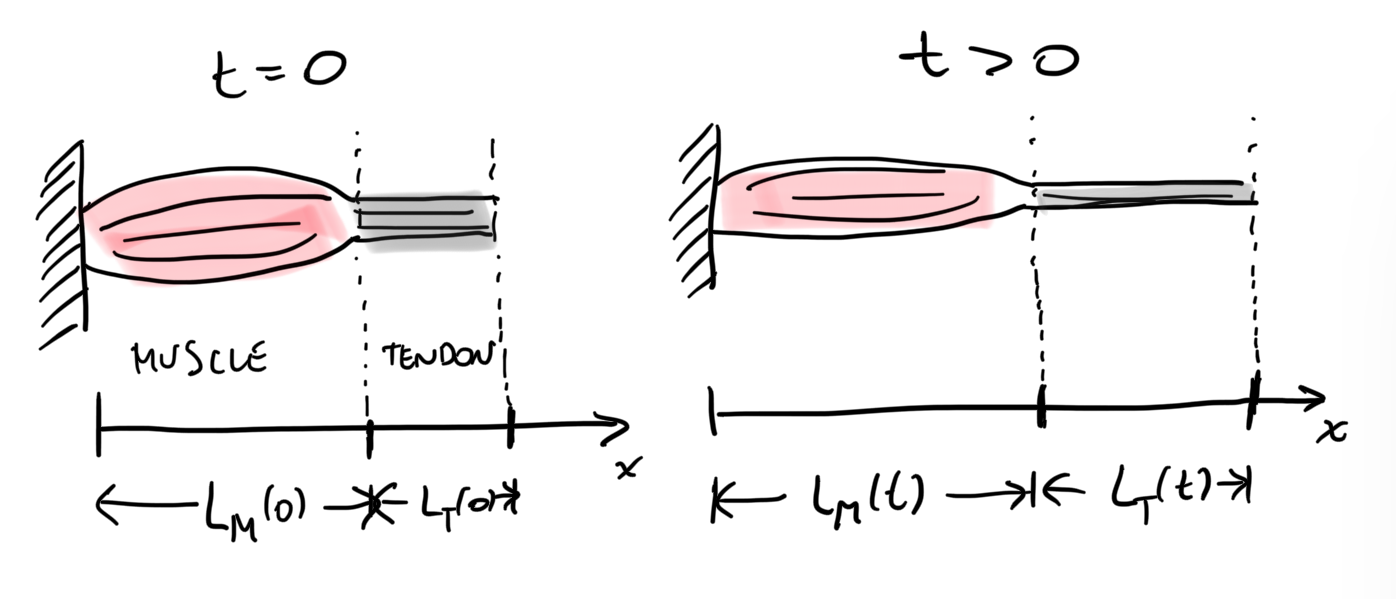
\includegraphics[width=0.9\textwidth]{mtu_sketch.jpeg}
    \caption{Sketch of an MTU (nicer version to come).}
    \label{fig:mtu_sketch}
\end{figure}

Let us develop a mathematical model of a dynamically contracting one-dimensional muscle tendon unit, such as the one depicted in Figure \ref{fig:mtu_sketch}. Denote by $L_M = L_M(t)$ and $L_T= L_T(t)$ the muscle and tendon lengths, respectively, at time $t \geq 0$. Moreover, denote by $L = L(t)$ the total length of the MTU which satisfies $L_M(t) + L_T(t) = L(t)$ for any time $t \geq 0$.

\subsection{Main concepts}

We define the \textit{muscle stretch} $\lambda_M$, the \textit{muscle strain} $\varepsilon_M$, and the \textit{muscle strain rate} $\depsilon_M$ as
\begin{equation} \label{eq:def_stretch_strain_rate_muscle}
    \lambda_M := \dfrac{L_M}{l_M^{opt}}, \qquad \varepsilon_M := \lambda_M - 1, \qquad \depsilon_M = \dfrac{1}{\depsilon_0} \der{\lambda_M}{t} = \dfrac{1}{l_M^{opt} \, \depsilon_0} \der{L_M}{t},
\end{equation}
where $l_M^{opt}$ is the \textit{optimal muscle length} and $\depsilon_0$ is the maximum unloaded shortening strain rate. Similarly, we can define the \textit{tendon stretch} $\lambda_T$ and \textit{tendon strain} $\varepsilon_T$ as
\begin{equation}
    \lambda_T := \dfrac{L_T}{l_T^{opt}}, \qquad \varepsilon_T := \lambda_T - 1.
\end{equation} 
The \textit{optimal tendon length} $l_T^{opt}$ can be computed from the \textit{optimal MTU length} $l_{MTU}^{ten}$ as  $l_T^{opt} = l_{MTU}^{opt} - l_M^{opt}$. For now, the reader can consider these quantities as given, however, they will be discussed more in detail in Section \ref{sec:optimal_muscle_length}.

\subsection{Hill's muscle model}

\begin{figure}
    \centering
    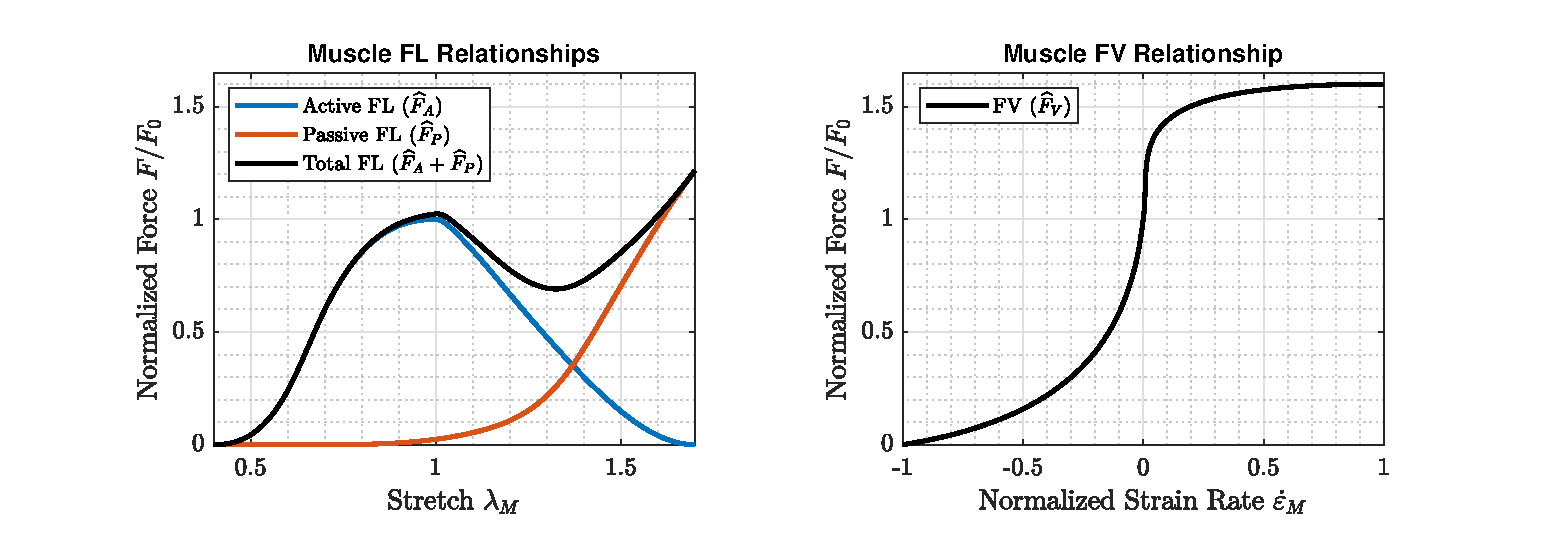
\includegraphics[width=\textwidth]{plot_FL_FV.eps}
    \caption{Force-length (FL) and force-velocity (FV) relationships that are part of Hill's muscle model \eqref{eq:Hill_force}. \label{fig:plot_FL_FV}}
\end{figure}

In a simple model, such as the one shown in Figure \ref{fig:muscle_models_1D}A, muscle can be thought as a one-dimensional spring containing a contractile element (CE) and a parallel elastic element (PEE). The first one is related to the force produced by actin-myosin interactions during activation, whereas the latter is related to passive components of the muscle fibre (such as titin), which act to prevent overstretching of the sarcomeres that form the muscle fibre. The muscle force $F_M$ in this case is given by Hill's equation \cite{Zajac1989},
\begin{equation} \label{eq:Hill_force}
    F_{Hill}(\lambda_M, \depsilon_M) = F_0 \Big\{ a(t) \widehat{F}_A(\lambda_M) \widehat{F}_V(\depsilon_M) + \widehat{F}_P(\lambda_M) \Big\}.
\end{equation}
In this expression, known as the standard \textit{Hill's muscle model}:
\begin{enumerate}
    \item The maximum isometric force, $F_0$, is the maximum force that a muscle can produce during an isometric contraction (that is, a \textit{fixed}-length contraction). This force is achieved when the length of the muscle $L_M$ is exactly the optimal muscle length $l_M^{opt}$. Therefore, assuming no pennation, it can be computed as:
    \begin{equation}
        F_0 = \sigma_0 \cdot PCSA_0 = \sigma_0 \cdot \dfrac{V_{0,M}}{l_M^{opt}},
    \end{equation}
    where $\sigma_0$ is the maximum isometric stress of muscle tissue, $PCSA_0$ is the optimal physiological cross-sectional area (PCSA), and $V_{0,M}$ is the muscle volume.
    \item The time-dependent activation function, $a = a(t)$, characterizes the influx of $\mathrm{Ca}_2^+$ ions that trigger the formation of cross-bridges between actins and myosins within sarcomeres. This function can be computed given an excitation $u(t)$ using Zajac's equation \cite{Zajac1989}:
    \begin{equation} \label{eq:zajac}
        \dfrac{da}{dt} + \dfrac{a(t)}{\tau_{act}} \left( \beta + (1-\beta)u(t) \right) = \dfrac{u(t)}{\tau_{act}}.
    \end{equation}
    \item The functions $\widehat{F}_A = \widehat{F}_A(\lambda_M)$ and $\widehat{F}_V = \widehat{F}_V(\depsilon)$ are known respectively as the active \textit{force-length} (FL) and \textit{force-velocity} (FV) relationships. They are related to the CE of the model and describe the force produced due to actin-myosin interactions during activation. These are normalized functions, meaning that $\widehat{F}_A(1) = 1$ and $\widehat{F}_V(0) = 1$.
    \item The function $\widehat{F}_P = \widehat{F}_P(\lambda_M)$ is known as the passive FL relationship. It is related to the PEE and describes the force produced by passive components of the muscle fibre (such as titin), which act to prevent overstretching of the sarcomeres.
\end{enumerate} 

%\begin{figure}
%    \centering
%    \begin{tikzpicture}[square/.style={regular polygon,regular polygon sides=4}]
%        \node[inner sep=0pt] at (0,0)
%            {\hspace{-3.5em}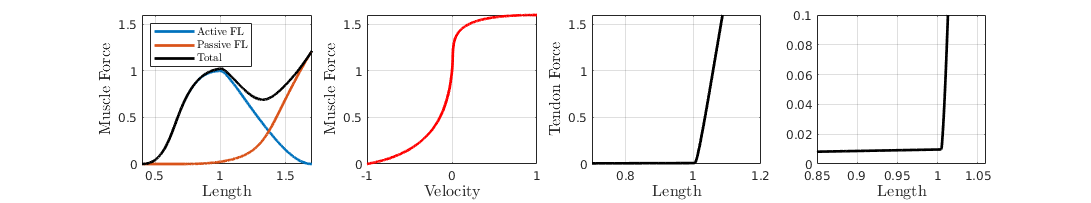
\includegraphics[width=1.18\textwidth]{force-curves-1D.png}};
%        \node at (1.8,-1) [square,draw] {\large \phantom{A}};
%        \draw[->] (2.2, -1) -- (3.8,-0.8);
%    \end{tikzpicture}
%    \caption{Force-relationships in use.}
%    \label{fig:force_curves_1D}
%\end{figure}

The force relationships $\widehat{F}_A$, $\widehat{F}_V$, and $\widehat{F}_P$ are typically fit from experimental data obtained through tensile experiments, and therefore do not have a standard expression. For this particular set of experiments, we use least-squares fits of the B\'{e}zier curves used by Ross et al. \cite{RossWakeling2016Multibody}. This allows us to evaluate the force directly given a stretch $\lambda_M$ without the need for solving a nonlinear equation, as is the case for B\'{e}zier curves (albeit with a minor loss of accuracy since the B\'{e}zier curves are already fit from experimental data). 
We show these curves in Figure \ref{fig:plot_FL_FV} and give their exact definitions in Appendix \ref{app:force_relationships}.

\begin{figure}
    \centering
    \begin{tikzpicture}
        \centering
        \node at (-2.8,1) {\huge \textbf{A}};
        \node[inner sep=0pt] at (0,0)
            {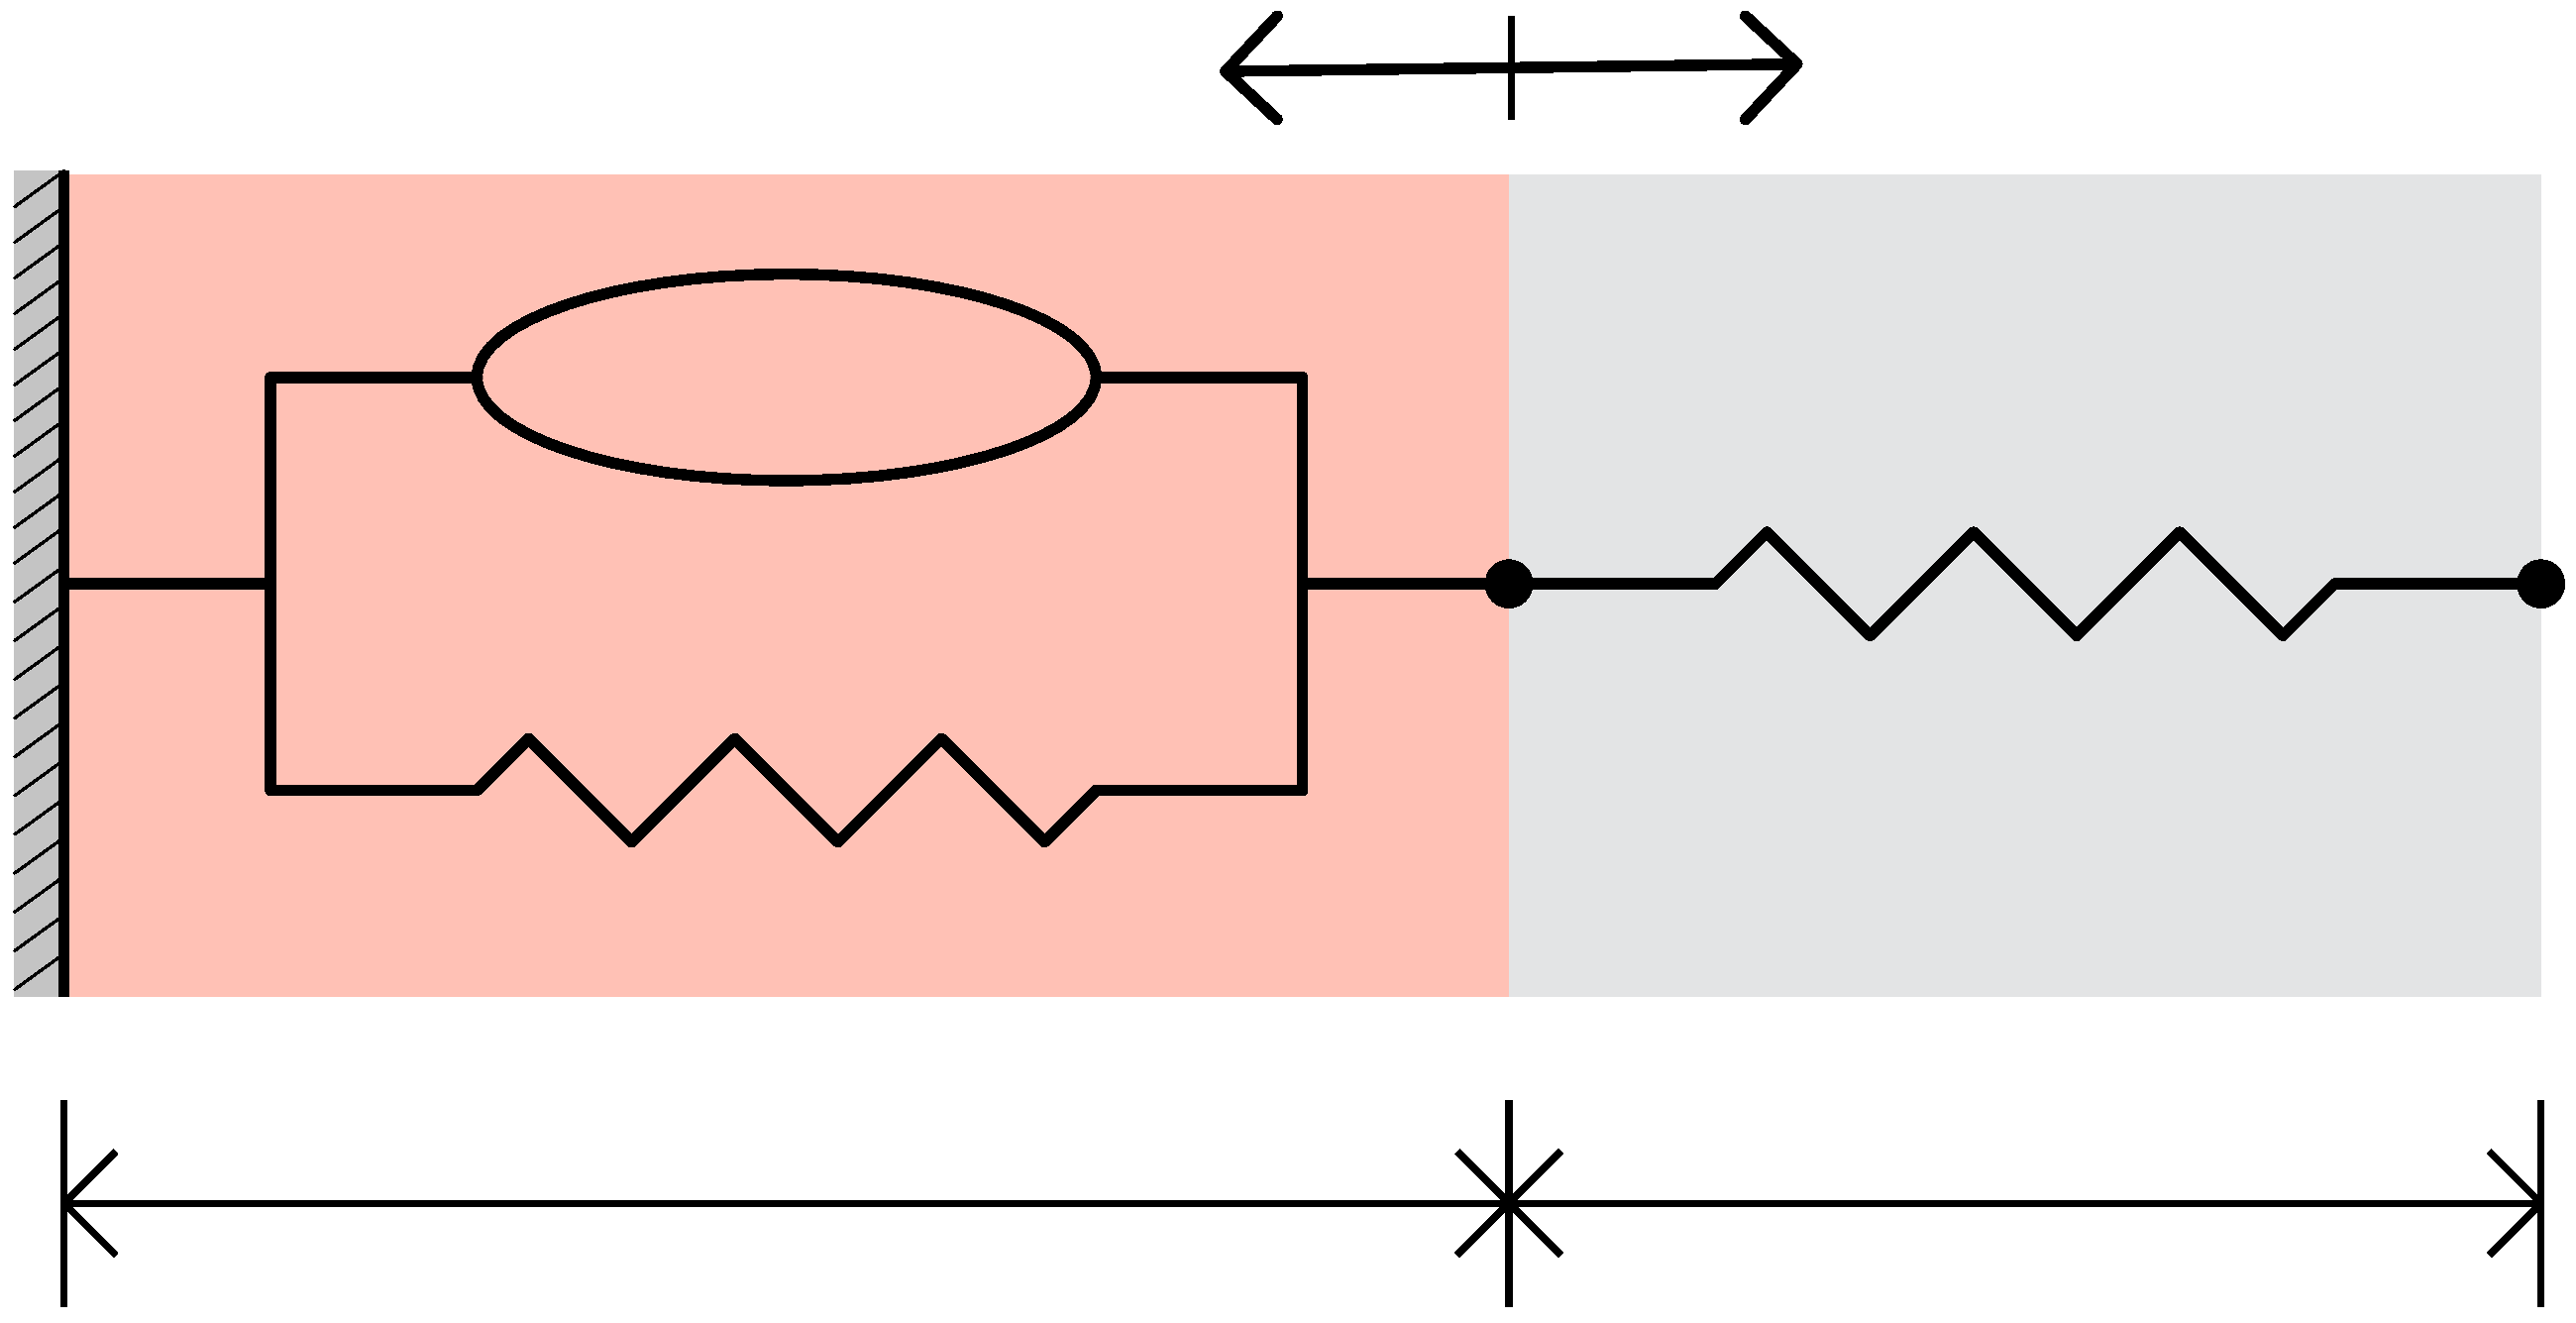
\includegraphics[width=0.3\textwidth]{hill-massless.eps}};
        \node at (-0.92,0.5) {\footnotesize CE};
        \node at (-0.92, -0.47) {\footnotesize PEE};
        \node at (1.33,-0.2) {SEE};
        \node at (-0.92, -1.25) {\footnotesize $L_M$};
        \node at (1.33, -1.25) {\footnotesize $L_T$};
        \node at (0.1, 1.45) {\footnotesize $\vec{F}_M$};
        \node at (0.7, 1.45) {\footnotesize $\vec{F}_T$};
    \end{tikzpicture}
    \hspace{0.5em}
    \begin{tikzpicture}
        \centering
        \node at (-4.5,1) {\huge \textbf{B}};
        \node[inner sep=0pt] at (0,0)
            {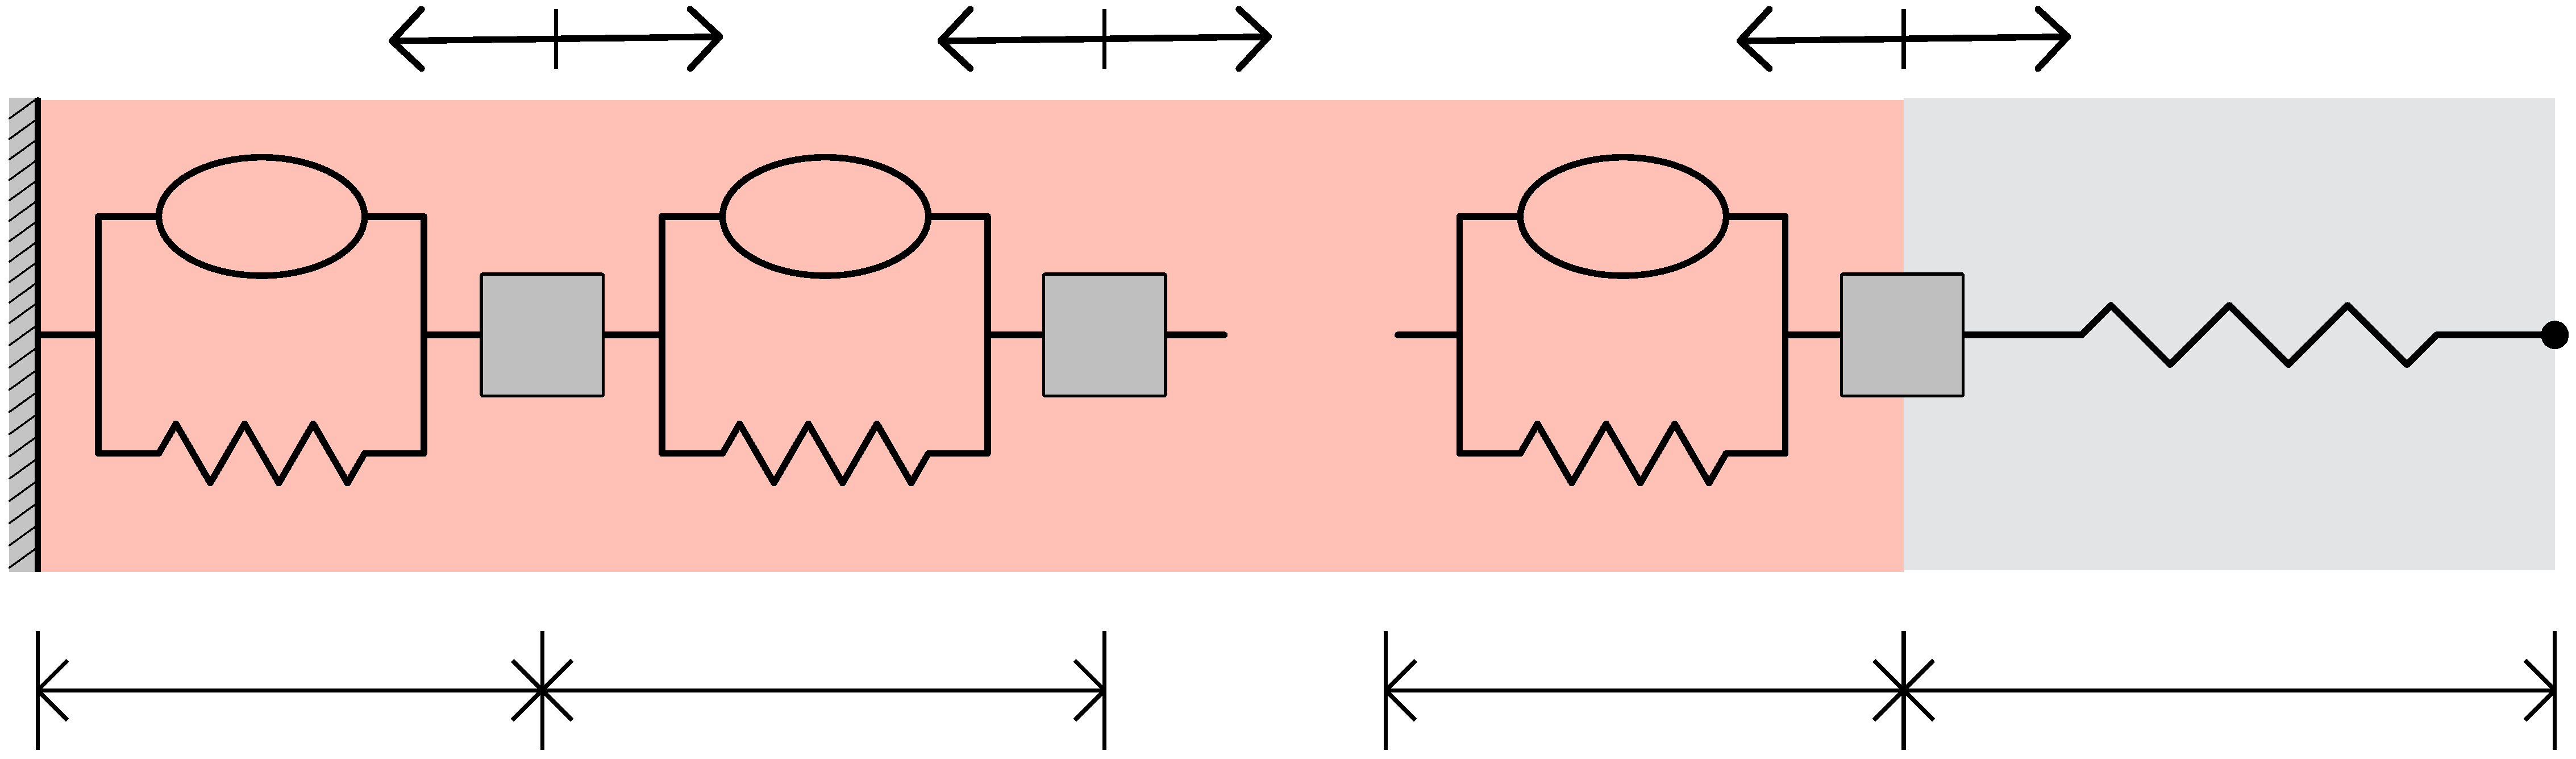
\includegraphics[width=0.525\textwidth]{hill-mass-enhanced.eps}};
        \node at (-2.31, 0.1) {\tiny $m_1$};
        \node at (-2.85, 1.44) {\tiny $-$};
        \node at (-0.56, 0.1) {\tiny $m_2$};
        \node at (-1.15, 1.44) {\tiny $-$};
        \node at (1.94, 0.1) {\tiny $m_{\hspace{-0.15em}N}$};
        \node at (-3.2, 0.5) {\tiny CE$_1$};
        \node at (-3.2, -0.5) {\tiny PEE$_1$};
        \node at (-3.2, -1.26) {\footnotesize $l_1$};
        \node at (-1.45, 0.5) {\tiny CE$_2$};
        \node at (-1.45, -0.5) {\tiny PEE$_2$};
        \node at (-1.45, -1.26) {\footnotesize $l_2$};
        \node at (1.08, 0.5) {\tiny CE$_{\hspace{-0.15em}N}$};
        \node at (1.08, -0.5) {\tiny PEE$_{\hspace{-0.15em}N}$};
        \node at (1.08, -1.26) {\footnotesize $l_N$};
        \node at (3.05, -0.2) {\tiny SEE};
        \node at (3.05, -1.26) {\footnotesize $L_T$};
        \node at (-2.6, 1.45) {\footnotesize $\vec{F}_1$};
        \node at (-2.0, 1.45) {\footnotesize $\vec{F}_2$};
        \node at (-0.9, 1.45) {\footnotesize $\vec{F}_2$};
        \node at (-0.3, 1.45) {\footnotesize $\vec{F}_3$};
        \node at (1.65, 1.45) {\footnotesize $\vec{F}_N$};
        \node at (1.38, 1.44) {\tiny $-$};
        \node at (2.25, 1.45) {\footnotesize $\vec{F}_T$};
        \node at (0.1,0.14) {\footnotesize $\dots$};
        \node at (-0.1,-1.0) {\footnotesize $\dots$};
    \end{tikzpicture}
    \caption{(A) A simple Hill-type model of the MTU (muscle region in pink, tendon region in grey) using massless springs. Depicted here are the (active) contractile element (CE), the passive elastic element (PEE), and the series elastic element (SEE) representing the tendon. (B) A multi-body model of the MTU that does not neglect the mass of the muscle, which is equally distributed throughout the muscle segment.}
    \label{fig:muscle_models_1D}
\end{figure}

\begin{figure}
    \centering
    \begin{tikzpicture}[square/.style={regular polygon,regular polygon sides=4}]
        \node[inner sep=0pt] at (0,0)
            {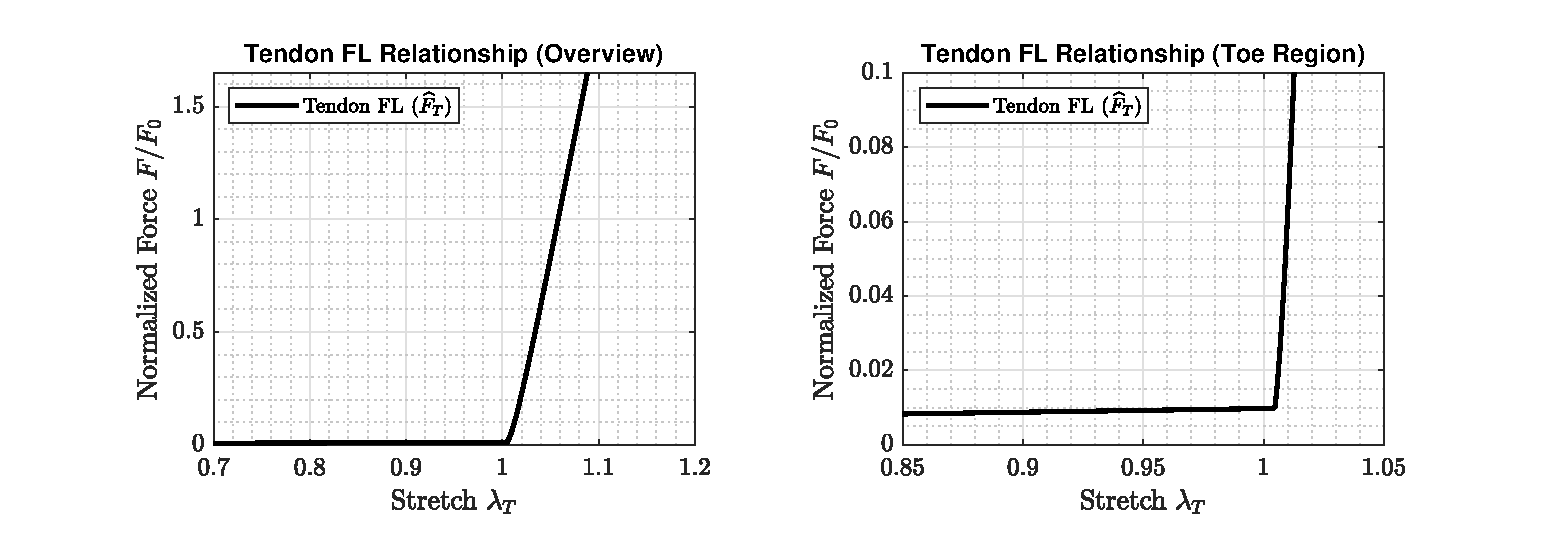
\includegraphics[width=\textwidth]{plot_FT.eps}};
        \node at (-2.7,-1.6) [square,draw] {\huge \phantom{A}};
        \draw[->] (-2.17, -1.6) -- (1.3,-1.4);
    \end{tikzpicture}
    \caption{Tendon FL relationship (left) with its toe region shown in detail (right). \label{fig:plot_FT}}
\end{figure}

%\begin{circuitikz}
    %ground
    %\pattern[pattern=north east lines] (0,0) rectangle (7,.25);
    %\draw[thick] (0,.25) -- (7,.25);
    
    %\draw (3,.25) to[spring, l=$k$] (3,2);
    %\draw (4,.25) to[damper, l_=$b$] (4,2);
    %\draw[fill=gray!40] (2.5,2) rectangle (4.5,3);
    %\node at (3.5,2.5) {$m$};
    
    %\draw[thick, ->] (3.5,4) -- (3.5,3);
    %\node at (3.75,3.75) {$F$};   
%\end{circuitikz}

%\begin{circuitikz}
    
    %\pattern[pattern=north east lines] (0,0) rectangle (0.2, 2);
    %\draw[thick] (0.2, 0) -- (0.2, 2);
    %\draw (0.2, 1) -- (0.8, 1);
    %\draw (0.8, 1) -- (0.8, 1.5) -- (1.3, 1.5);
    %\draw (1.9, 1.5) ellipse (6mm and 3mm);
    %\draw (2.5, 1.5) -- (3.0, 1.5);
    %\draw (0.8, 1) -- (0.8, 0.5) -- (1.0, 0.5);
    %\draw (1.0, 0.5) to[R] ++(1.8, 0) -- (3.0, 0.5);
    %\draw (3.0, 0.5) -- (3.0, 1.5);
    %\draw (3.0, 1.0) -- (3.6, 1.0);

%\end{circuitikz}

\subsection{Massless and mass-enhanced models of the MTU}

For the model in Figure \ref{fig:muscle_models_1D}A, the muscle force $F_M \equiv F_{Hill}$ is balanced by the tendon force $F_T$ (shown in Figure \ref{fig:plot_FT}) at all times, that is:
\begin{equation} \label{eq:massless_model}
    F_M(\lambda_M, \depsilon_M) = F_T(\lambda_T), \quad t > 0.
\end{equation}
This first-order implicit ODE, which we refer to as the \textit{massless} model, represents a model of the MTU in which the mass of the muscle is not taken into consideration. While this may seem like an outrageous simplification of the problem, it is actually what is being solved in the backend of many popular biomechanics software, such as OpenSim \cite{Delp2007OpenSim}. Hence, \textbf{this model's absence of mass raises the question of whether including mass has any effect in the prediction of the dynamics of the system}. 

In an attempt to answer the previous question, based on the work by G\"{u}nther et al. \cite{Gunther2012}, Ross et al. \cite{Ross2018}, and Ross \& Wakeling \cite{RossWakeling2016Multibody, RossPaper4}, Chen \cite{EvanThesis} has put forward a muscle model in which the mass of the muscle is equally distributed into $N$ segments (see Figure \ref{fig:muscle_models_1D}B), forming a multi-body system with $N$ bodies. The dynamics in this model, which we refer to as the \textit{mass-enhanced} model, are given by the set of second-order ODEs:
\begin{subequations} \label{eq:massenhanced_model}
    \begin{align}
        m_1 \ddot{u}_1 &= F_2(\lambda_2, \depsilon_2) - F_1(\lambda_1, \depsilon_1), \\
        m_2 \ddot{u}_2 &= F_3(\lambda_3, \depsilon_3) - F_2(\lambda_2, \depsilon_2), \\
        &\hspace{0.6em} \vdots \notag \\
        m_N \ddot{u}_N &= F_T(\lambda_T) - F_N(\lambda_N, \depsilon_N).
    \end{align}
\end{subequations}
Here, $m_1 = m_2 = \dots = m_N = m_{mus}/N$, where the mass of the muscle $m_{mus}$ depends on its (initial) volume $V_{0,M}$ through the (initial) density of muscle tissue $\rho_0$, which is assumed to be constant across mammalian species \cite{MendezKeys1960}:
\begin{equation}
    \rho_0 = \dfrac{m_{mus}}{V_{0,M}} = 1,060 \ \dfrac{\text{kg}}{\text{m}^3}.
\end{equation}
Moreover, the muscle volume $V_{0,M}$ is estimated using a formula depending on the subject's height $H$ and mass $W$ \cite{Hansfield2014}:
\begin{equation}
    V_{0,M} = V_0 \cdot \chi_M, \quad V_0 = (47WH + 1285) \cdot 10^{-6},
\end{equation}
where $\chi_M$ is the fraction of individual muscle relative to the volume of one lower leg $V_0$ (see Table \ref{tab:1d-parameters}).

In turn, $u_i$ denotes the displacement of the $i$-th segment, that is,
\begin{equation}
    u_i = x_i - x_i^0, \quad i=1,\dots,N,
\end{equation}
where $x_i$ is the position of the $i$-th segment and $x_i^0$ denotes its initial position. Furthermore, $\lambda_i$ and $\depsilon_i$ denote the segment stretch and strain rate of the $i$-th segment, respectively
\[
\lambda_i = \dfrac{l_i}{l_s^{opt}} = \dfrac{l_i}{l_M^{opt}/N}, \quad \depsilon_i = \dfrac{\dot{\lambda_i}}{\depsilon_0}, \quad i = 1,\dots,N.
\]
These stretches and strain rates can be written in terms of the displacements $u_i$ as:
\begin{equation}
    \lambda_1 = \dfrac{u_1 + l_s^0}{l_s^{opt}}, \quad \lambda_2 = \dfrac{u_2-u_1 + l_s^0}{l_s^{opt}}, \quad \dots \quad, \lambda_N = \dfrac{u_N-u_{N-1} + l_s^0}{l_s^{opt}},
\end{equation}
and
\begin{equation}
    \depsilon_1 = \dfrac{\dot{u}_1}{l_s^{opt} \depsilon_0}, \quad \depsilon_2 = \dfrac{\dot{u}_2-\dot{u}_1}{l_s^{opt} \depsilon_0}, \quad \dots \quad, \depsilon_N = \dfrac{\dot{u}_N - \dot{x}_{N-1}}{l_s^{opt} \depsilon_0},
\end{equation}
with $l_s^0 := L_M(0)/N$ is the initial length of each segment and $l_s^{opt} = l_M^{opt}/N$. In particular, the muscle length can be computed directly from the position of the last mass, i.e. $L_M = x_N$.

To complete the description of the massless and mass-enhanced models (equations \eqref{eq:massless_model} and \eqref{eq:massenhanced_model}, respectively), we have to provide the optimal muscle length $l_M^{opt}$, as well as the initial muscle length $L_M(0)$. The latter is sufficient to provide initial conditions for the system \eqref{eq:massenhanced_model} (assuming that the system of $N$ bodies is initially at rest, i.e. $\dot{u}_i(0) = 0$). Because we will be working with experimentally-obtained data and force relationships that are particular to this study, $l_M^{opt}$ and $L_M(0)$ can only be \textit{estimated} from the literature, so an optimized value must be computed to ensure simulations start from static equilibrium. This topic will be discussed in the next section.

\begin{table}
    \centering
    \begin{tabular}{|lp{5cm}|l|l|}\hline
         & Description & Value & References \\\hline
        $\sigma_0$ & Muscle maximum isometric stress & 225 kPa & \cite{Medler2002, Powell1984}\\\hline
        $\depsilon_0$ & Muscle maximum unloaded shortening strain rate & \makecell[l]{5 s$^{-1}$ (walking, running) \\ 10 s$^{-1}$ (cycling)} & \cite{WakeingLee2012} \\\hline
        $\tau_{act}$ & Time constant for activation & \makecell[l]{0.045 s (walking, running) \\ 0.025 s (cycling)} & \cite{Dick2017} \\\hline
        $\beta$ & Ratio of $\tau_{act}$ to deactivation time constant & 0.6 &\cite{Dick2017} \\\hline
        $\chi_M$ & Volume fraction of muscle with respect to that of one lower leg & \makecell[l]{MG: 0.0362 \\ VM: 0.0606 \\ ST: 0.026} & \cite{Hansfield2014} \\\hline
        $r_M$ & Muscle-to-MTU length ratio & \makecell[l]{MG: 0.54 \\ VM: 0.84 \\ ST: 0.70 } & \cite{Kovacz2020,OBrien2010}\\\hline
        $l_{MTU}^{opt}$ & Optimal MTU length & \makecell[l]{Subject 1 (walking, running):\\ \hspace{1em} MG: 0.3910 m \\ \hspace{1em} VM: 0.2770 m \\ \hspace{1em} ST: 0.4122 m \\ Subject 2 (cycling):\\ \hspace{1em} MG: 0.3952 m \\ \hspace{1em} VM: 0.2171 m \\ \hspace{1em} ST: 0.4381 m} & \cite{EvanThesis} \\\hline
    \end{tabular}
    \caption{List of parameters for the mass-enhanced and massless models. The muscles listed in the table are the \textit{medial gastrocnemius} (MG), \textit{semitendinosus} (ST), and \textit{vastus medialis} (VM).}
    \label{tab:1d-parameters}
\end{table}

\subsection{Optimal muscle and tendon length} \label{sec:optimal_muscle_length}

The optimal muscle length, $l_M^{opt}$, is the length at which myofilament overlap is optimal\footnote{This happens at sarcomere lengths of about 2.6-2.8 $\mu$m in human muscle and 2.0-2.2 $\mu$m in frog muscle \cite{FridenLieber1998}.} and force production is maximal \cite{FridenLieber1998}, that is, when $F_M = F_0$ at $L_M = l_M^{opt}$. When the MTU is fixed at this length (that is, $L = l_{MTU}^{opt}$), muscle and tendon forces balance:
$F_M(1) = F_0 = F_T(1)$. This means that the definition of $l_M^{opt}$ depends on the FL relationship, which is particular to the muscle in study. Therefore, any quantity obtained from the literature can only be considered an \textit{estimate}. Denote the estimated optimal muscle and tendon lengths respectively by $\widetilde{l_M^{opt}}$ and $\widetilde{l_M^{opt}}$, which are given by:
\begin{equation}
	\widetilde{l_M^{opt}} := l_{MTU}^{opt} r_M, \qquad \widetilde{l_T^{opt}} := l_{MTU}^{opt}(1-r_M).
\end{equation}
Here, $l_{MTU}^{opt}$ is the optimal MTU length (given) and $r_M$ is the muscle-to-MTU-length ratio (see Table \ref{tab:1d-parameters}). Furthermore, assume that this estimate as a deviation $\Delta l_M^{opt}$ from the true value $l_M^{opt}$, i.e.
\begin{equation}
    l_M^{opt} = \widetilde{l_M^{opt}} + \Delta l_M^{opt}, \qquad l_T^{opt} = \widetilde{l_T^{opt}} - \Delta l_M^{opt}.
\end{equation}
Since muscle and tendon force balance at optimal MTU length, and assuming that the muscle is inactive ($a=0$) and $F_T = F_0 \widehat{F}_T$, the true values $l_M^{opt}$ and $l_T^{opt}$ can be obtained by solving the following equation for the error $\Delta l_M^{opt}$:
\begin{equation} \label{eq:calibration_1}
    \widehat{F}_P\left( \dfrac{\widetilde{l_M^{opt}}}{\widetilde{l_M^{opt}} + \Delta l^{opt}} \right) = \widehat{F}_T \left( \dfrac{\widetilde{l_T^{opt}}}{\widetilde{l_T^{opt}} - \Delta l^{opt}} \right).
\end{equation}

\subsection{Initial muscle length}

Similar to the computation of optimal muscle and tendon lengths, to ensure the simulation begins from static equilibrium, we assume that the given initial MTU length $L(0)$ only provides estimates for the initial muscle and tendon lengths, that is:
\begin{equation}
    \widetilde{L_M(0)} = L(0) \cdot r_M, \quad \widetilde{L_T(0)} = L(0) \cdot (1-r_M).
\end{equation}
Furthermore, we assume that the true values for $L_M(0)$ and $L_T(0)$ are off by a factor of $\Delta L_M(0)$, that is, 
\begin{equation}
    L_M(0) =  \widetilde{L_M(0)} + \Delta L_M(0), \quad L_T(0) = \widetilde{L_T(0)} - \Delta L_M(0).
\end{equation}
Then, we can find the value of this correction by solving the equation
\begin{equation} \label{eq:calibration_2}
    F_P \left( \dfrac{\widetilde{L_M(0)} - \Delta L_M(0)}{l_M^{opt}}\right) = F_T \left( \dfrac{\widetilde{L_T(0)} + \Delta L_M(0)}{l_T^{opt}}\right).
\end{equation}
The corrections $\Delta l_M^{opt}$ and $\Delta L_M(0)$ are typically small and represent the correct setup of the locomotion experiment at the time of data collection.

\subsection{Scaling}

As mentioned in the introduction to this thesis, most of our knowledge in human biomechanics comes from experiments performed in small animals, such as frogs, rats, and cats. 
However, it is known that larger (thus heavier) muscles will yield more inertial effects than smaller ones, so the size difference should not always be neglected \cite{EvanThesis,Ross2018}. This motivates the consideration of scaled up versions of the muscles in study. In this way, a scaling factor of $s$ means that the MTU length will be scaled up by a factor of $s$, the physiological cross sectional area of muscle by a factor of $s^2$, the muscle volume by a factor of $s^3$, and so on. For example, in studies of gearing, the MG from young rats considered by Holt et al. \cite{Holt2016} had an average volume of $8.4906 \cdot 10^{-7} \ m^3$. In turn, the subject used in this study for walking and running tasks had a MG volume of about $2.3348 \cdot 10^{-4} \ m^3$. That is about 275 times the volume of the rat MG, equivalent to a scaling factor of about 6.5. In this study, we will use scales of 1 and 10.

\section{Experimental data: muscles and tasks in consideration} \label{sec:experimental_data}

\begin{figure}
    \centering
    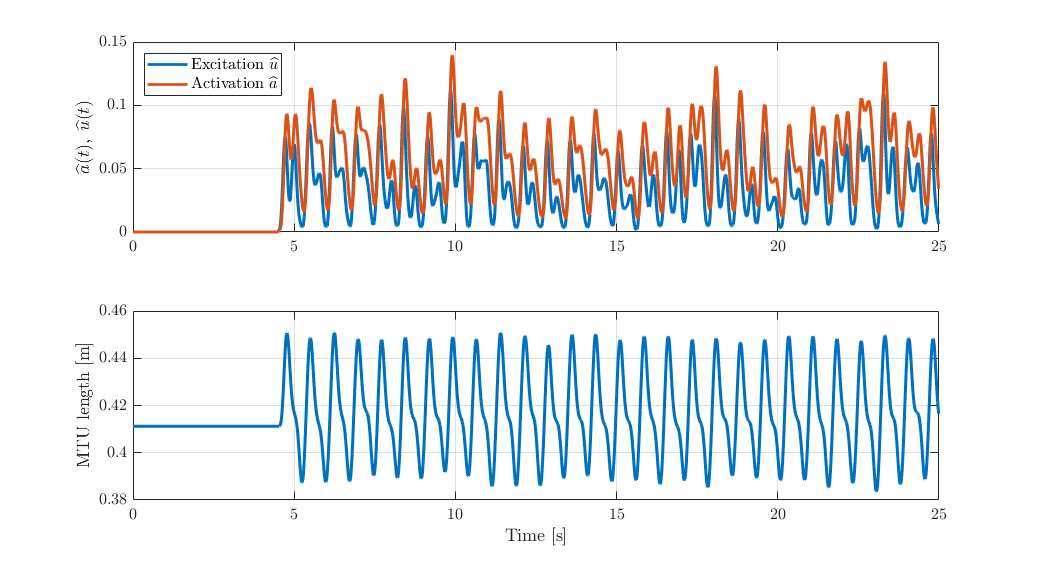
\includegraphics[width=\textwidth]{example-traces-activation-mtulength.png}
    \caption{Example traces of the data (muscle: ST, task: running) used as input for the one-dimensional massless and mass-enhanced models. In this case, the activation $\widehat{a}$ has been computed from the excitation $\widehat{u}$ using Zajac's ODE \eqref{eq:zajac}.}
    \label{fig:traces_act_mtu_length}
\end{figure}

We consider two subjects of equal mass (68 kg) and height (1.67 m) who were asked to perform a set of locomotion tasks: walking and running at their own pace \cite{EvanThesis}, and cycling at a cadence of 80 \si{s^{-1}} and a crank load of 26 N\hspace{0.1em}m \cite{Dick2016}. Moreover, we consider the muscle excitation $\widehat{u}(t)$ and MTU length $L(t)$ from three different muscles: medial gastrocnemius (MG), vastus medialis (VM), and semitendinosus (ST). Thus, nine different muscle-task combinations can be formed. An example of these data are shown in Figure \ref{fig:traces_act_mtu_length} for the ST during running. All data were recorded for a time span of 25 seconds. For more precise details on the experiment setup and data collection, we refer the reader to \cite{EvanThesis}.

%\begin{enumerate}
%    \item matlab solvers in use, tolerances
%    \item computational architectures
%\end{enumerate}

\section{Computational implementation}

Solvers for the massless \eqref{eq:massless_model} and mass-enhanced model \eqref{eq:massenhanced_model}, as well as for the Zajac ODE \eqref{eq:zajac} and the calibration steps \eqref{eq:calibration_1} and \eqref{eq:calibration_2} were implemented in \matlab using built-in routines. See Table \ref{tab:matlab_solvers} for a list of these solvers and the default parameters that were used. In particular, the ODE solvers are \textit{adaptive}, meaning that the time step size is controlled by absolute and relative tolerance requirements \cite{ShampineReichelt1997}. First, \texttt{ode45} is a single-step solver based on an explicit Runge-Kutta (4,5) formula (the Dormand-Prince pair \cite{DormandPrince1980}). It is typically used for non-stiff ODEs, such as Zajac's ODE \eqref{eq:zajac}. Next, \texttt{ode15s} is a variable-order, variable-step solver based on differentiation formulas of order 1 to 5 \cite{ShampineReichelt1997}. It is a multistep solver used for solving stiff ODEs, such as the mass-enhanced model \eqref{eq:massenhanced_model}. Finally, \texttt{ode15i} is similar to \texttt{ode15s}, but it is designed to solve fully implicit differential equations \cite{Shampine2002}, such as the massless model \eqref{eq:massless_model}.

The complete set of codes written for this study is available at:
\begin{center}
    \url{www.github.com/javieralmonacid/multibody-muscle-1d}.
\end{center} 

\begin{table}
    \centering
    \begin{tabular}{|l|c|c|c|c|}\hline
        Description & \matlab solver & AbsTol & RelTol & N \\\hline
        Zajac ODE \eqref{eq:zajac} & \texttt{ode45} & 1e-6 & 1e-3 & - \\\hline
        Parameter calibration \eqref{eq:calibration_1}, \eqref{eq:calibration_2} & \texttt{fzero} & - & - & - \\\hline
        Massless model \eqref{eq:massless_model} & \texttt{ode15i} & 1e-6 & 1e-6 & - \\\hline
        Mass-enhanced model \eqref{eq:massenhanced_model} & \texttt{ode15s} & 1e-10 & 1e-6 & 64 \\\hline
    \end{tabular}
    \caption{List of \matlab built-in solvers in use.}
    \label{tab:matlab_solvers}
\end{table}


\subsection*{A convergence test}

To have an idea on what to expect for the general results, and to evaluate the convergence of the solvers, let us perform an experiment using the MTU length and activation data from the ST muscle during running. Here, we fix the scale to $s=10$, the number of masses to $N=16$ (as used in \cite{EvanThesis,RossWakeling2016Multibody,RossPaper4}), the absolute tolerance to $10^{-10}$, and vary the relative tolerance from $10^{-2}$, $10^{-4}$, \dots down to $10^{-10}$. We show the results in Figure \ref{fig:multibody-reltol} for three representative seconds of output. Recall that no exact solution is available for this problem.

First, we observe that the muscle stretch $\lambda_M$ and the muscle strain rate $\depsilon_M$ are within the (generally accepted) operating ranges of human muscle, that is $\lambda_M \in [0.85, 1.15]$ and $\depsilon_M \in [-0.3, 0.3]$. Next, we notice that the muscle stretch contains minor oscillations when $\lambda_M < 1$. These are then amplified in the muscle strain rate as it varies from $\depsilon_M < 0$ to $\depsilon_M > 0$. Moreover, reducing the relative tolerance does not yield a better approximation (qualitatively speaking), even though the average time step size is indeed decreasing (see Figure \ref{fig:multibody-reltol-avg-deltat}). This is a sign that the solver is correctly resolving the primary unknowns, and that the apparent stiffness in the system is not tied to the time discretization, as we will see in the next section.

\begin{figure}
    \centering
    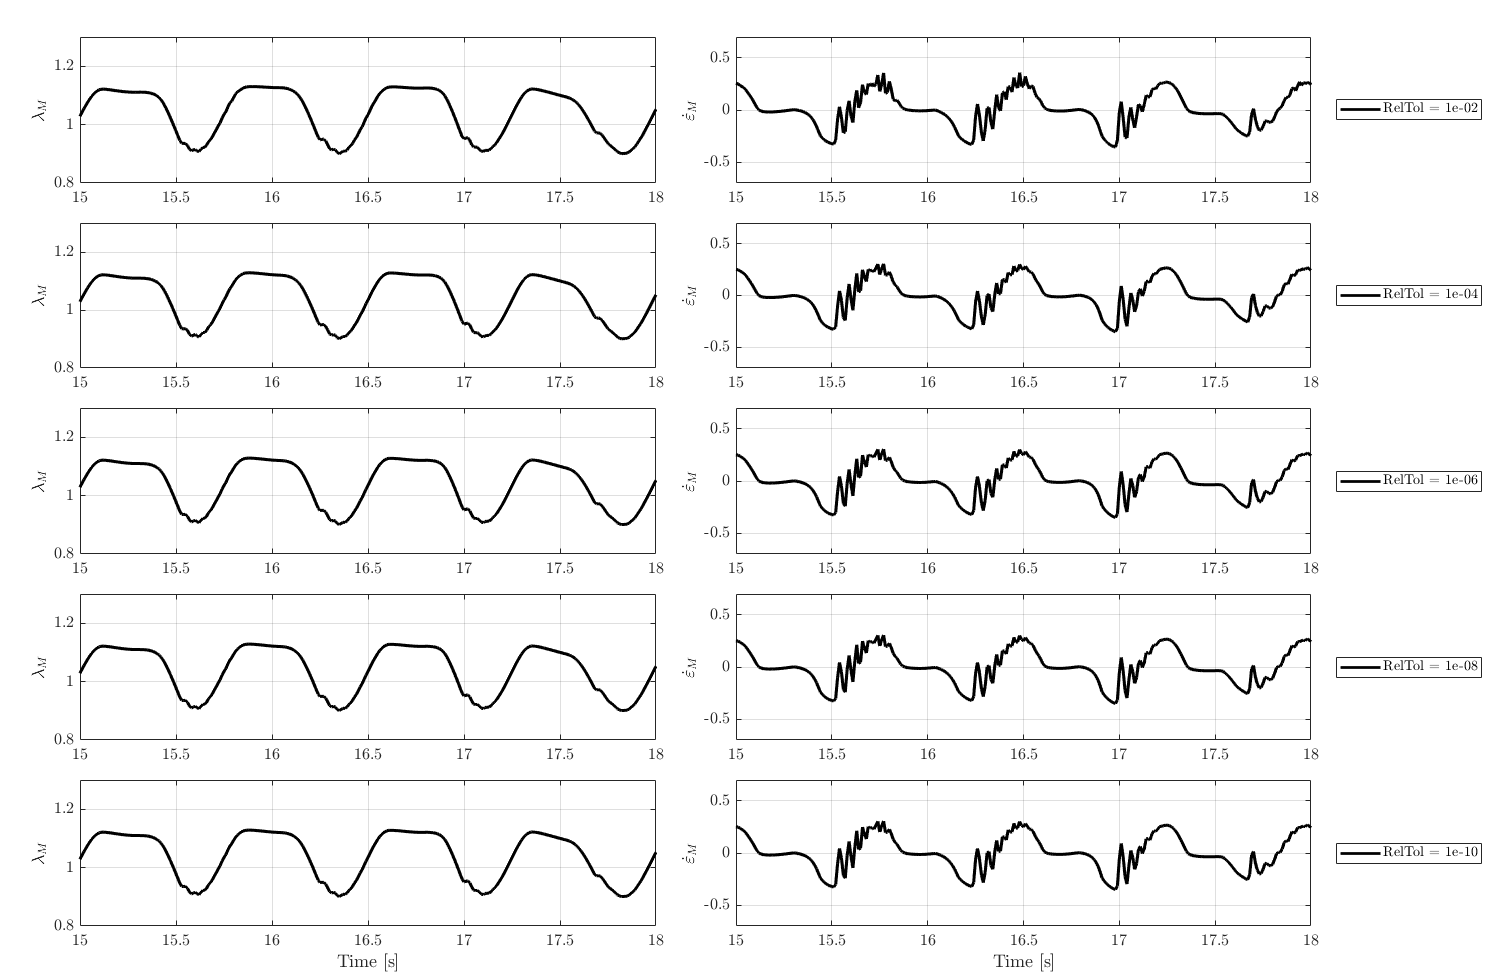
\includegraphics[width=\textwidth]{multibody-reltol-effect.png}
    \caption{Traces of muscle strains ($\lambda_M$) and strain rates ($\depsilon_M$) as the relative tolerance in the ODE solver is varied while the absolute tolerance is fixed to $10^{-10}$.}
    \label{fig:multibody-reltol}
\end{figure}

\begin{figure}
    \centering
    %\begin{tabular}{|l|c|c|c|c|c|}\hline
    %    RelTol & 1e-2 & 1e-4 & 1e-6 & 1e-8 & 1e-10 \\\hline
    %    Avg. $\Delta t$ (ms) & 2.9145 & 0.7197 & 0.2106 & 0.0791 & 0.0352 \\\hline
    %\end{tabular}
    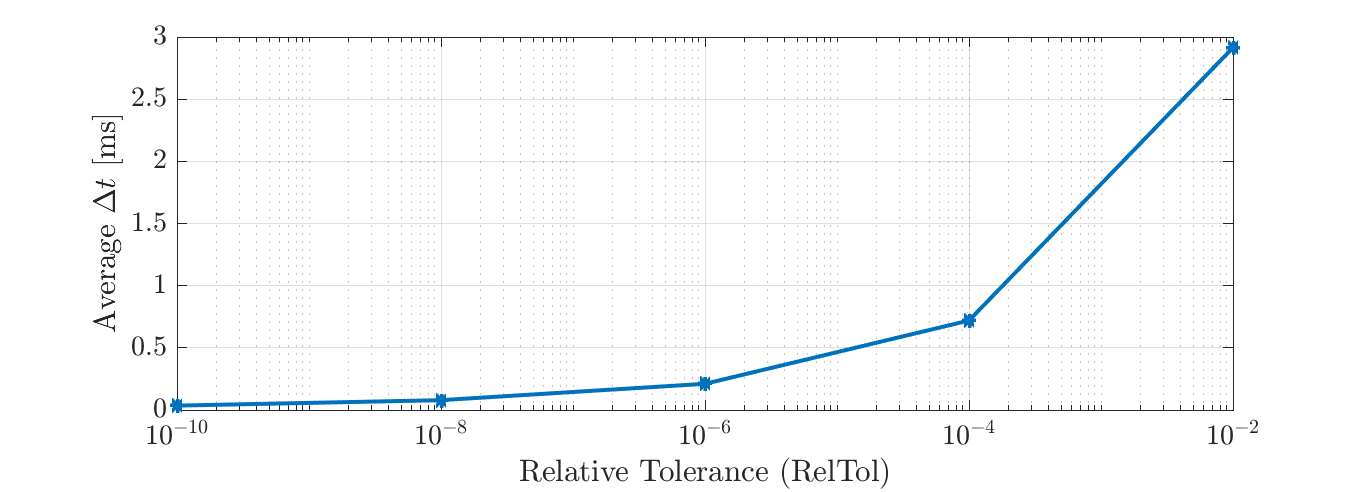
\includegraphics[width=\textwidth]{convergence_dt.png}
    \caption{Average time step size $\Delta t$ in the mass-enhanced model as the relative tolerance decreases while the absolute tolerance is fixed to $10^{-10}$.}
    \label{fig:multibody-reltol-avg-deltat}
\end{figure}


\section{Main results}

We perform simulations for all 9 muscle-task pairs at scales $s=1$ and $s=10$ using the solvers described in the previous section. Moreover, we focus on the behaviour of the ST during running. Finally, we analyze the impact of the number of the masses on the system in the quality of the output.

\subsection{Overall behaviour for different muscles and tasks}

In Figure \ref{fig:multibody_predicted_forces_1_10} we show the predicted normalized muscle force (i.e. $F_M/F_0$, see \eqref{eq:Hill_force}) using the massless and mass-enhanced ($N = 64$) models for three representative seconds of data. The input data in this case are MTU lengths and activation patterns from the three different muscles and the three different tasks specified in Section \ref{sec:experimental_data}. In line with the findings by Chen \cite{EvanThesis}, we observe negligible differences when $s=1$ (see Figure \ref{fig:multibody_predicted_forces_1_10}A) and significant differences when $s=10$ (up to 14\% RMSE difference for ST-running, see Figure \ref{fig:multibody_predicted_forces_1_10}B).

In general, when we scale the muscle 10 times its size (i.e. $s=10$), the mass-enhanced model can capture much sharper dynamics than the massless model. Moreover, the inertial effects can cause faster variations of muscle force (ST-walking), shifts in phase (VM-cycling), and differences of peak (local) force of above 100\% (ST-running). 

Computationally speaking, even though the dynamics of the MTU are, in general, smooth for all muscle-task pairs (see, for instance, Figure \ref{fig:traces_act_mtu_length}), the time that it takes to simulate the full 25 seconds of data varies significantly, not only depending on the model but also on the muscle and the task of choice. While the massless model finishes computation in about 1 to 5 seconds, the mass-enhanced model can easily take hours to compute a result (up to 5 hours for the ST muscle during running, see Table \ref{tab:multibody_computational_time}).

\begin{figure} 
    \centering
    \begin{tikzpicture}
        \node[inner sep=0pt] at (0,0)
            {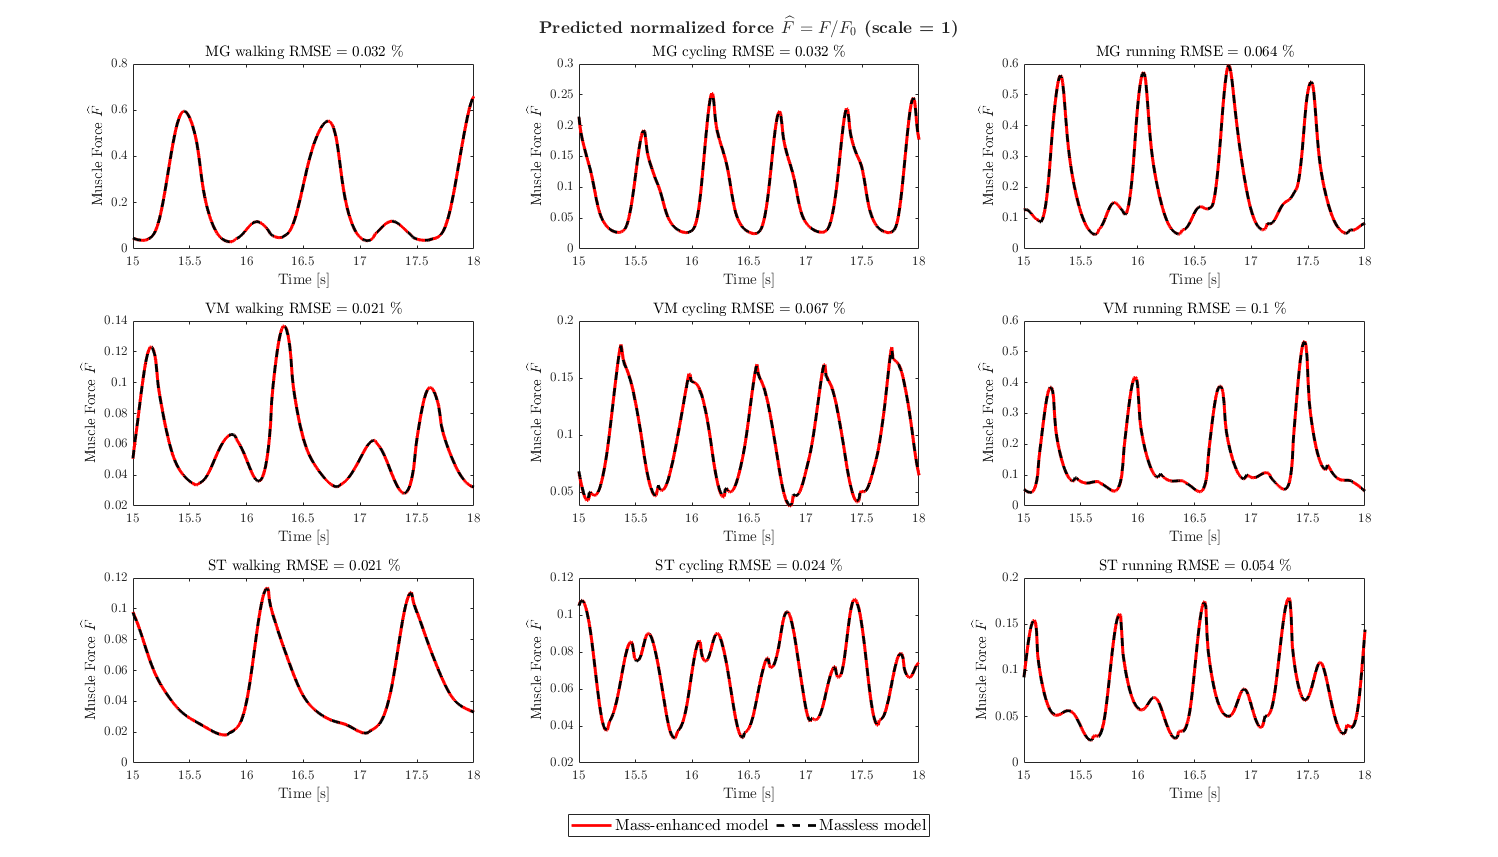
\includegraphics[width=\textwidth]{multibody-force-scale-1.png}};
        \node[inner sep=0pt] at (0,-9.5)
            {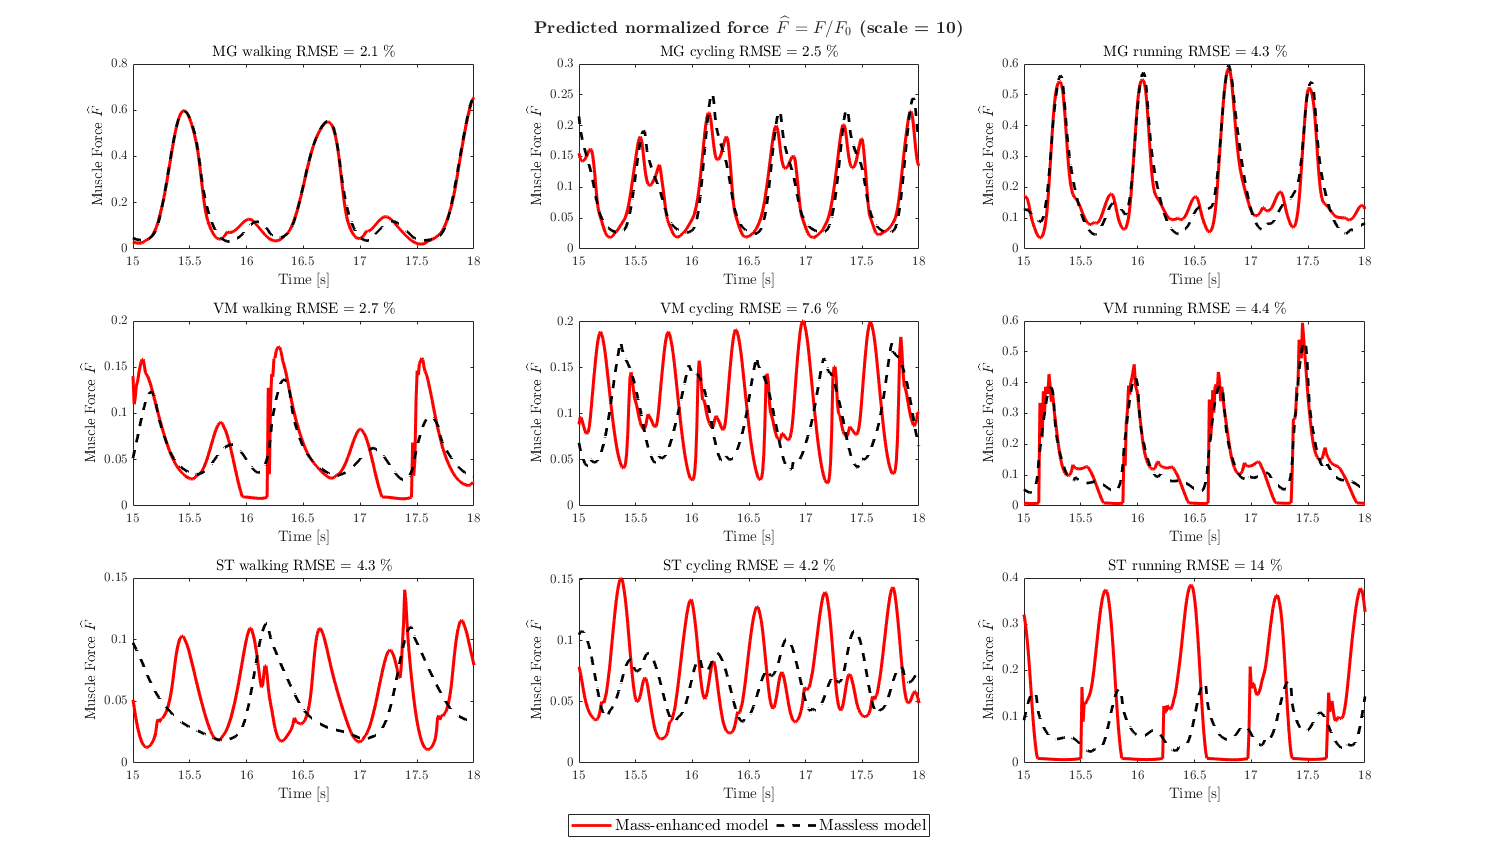
\includegraphics[width=\textwidth]{multibody-force-scale-10.png}};
        \node at (-7.5,4.5) {\huge \textbf{A}};
        \node at (-7.5,-5) {\huge \textbf{B}};
    \end{tikzpicture}
    \caption{Predicted (normalized) forces when the scaling parameter is unchanged (i.e. $s=1$; A) and when $s=10$ (B) for 9 different muscle-task combinations. RMSE computed using the data range shown in the figures.}
    \label{fig:multibody_predicted_forces_1_10}
\end{figure}

\begin{table} 
    \centering
    \begin{tabular}{|c|c|c|c|}\hline
        \multicolumn{4}{|c|}{scale = 1} \\\hline
        Muscle $\backslash$ Task & Walking & Cycling & Running \\\hline
        MG & 1.01 & 0.80 & 1.19 \\\hline
        VM & 2.28 & 1.33 & 2.79 \\\hline
        ST & 1.28 & 0.83 & 1.54 \\\hline\hline
        \multicolumn{4}{|c|}{scale = 10} \\\hline
        Muscle $\backslash$ Task & Walking & Cycling & Running \\\hline
        MG & 1.15 & 0.99 & 1.79 \\\hline
        VM & 2.07 & 3.29 & 3.70 \\\hline
        ST & 2.54 & 0.90 & 5.10 \\\hline
    \end{tabular}
    \caption{Computation times (in hours) for each muscle-task combination at scales 1 and 10 for the full 25 seconds of available data using the mass-enhanced model.}
    \label{tab:multibody_computational_time}
\end{table}

\subsection{Dynamics of the ST during running}

In view of the previous results, we decide to have a closer look at the behaviour of the ST muscle during running. In particular, we show traces of excitation, activation, muscle length, tendon length, muscle strain rate, and normalized muscle force for $s=1$ and $s=10$ in Figure \ref{fig:multibody_traces_ST_running}. Here, the excitation is given from the experimental data, the activation is computed based on this excitation using \eqref{eq:zajac}, and the rest of the variables are computed by the solver. In particular, the muscle force is equal to the computed tendon force, since we are assuming that the tendon transmits the entirety of the force generated by muscle. 

These results show that the tendon acts as a strut when $s=1$, but it is no longer the case for $s=10$. Indeed, tendon strains of up to -20\% are observed, and they produce sharp variations of strain rate (and ultimately force) that the massless model cannot capture. Another important feature is that, when $s=10$, we observe a development of impulsive forces when transitioning from $\depsilon_M < 0$ to $\depsilon_M > 0$. This is something that has not been described previously (cf. \cite{EvanThesis,Ross2018}) because the dynamics in these works are much smoother. We also note that the results in Figure \ref{fig:multibody_traces_ST_running} were computed using $N=64$ masses (see Table \ref{tab:matlab_solvers}) because the simulation was not fully resolved when $N=16$ masses were used. 

\begin{figure} 
    \centering
    \hspace*{-5.5em}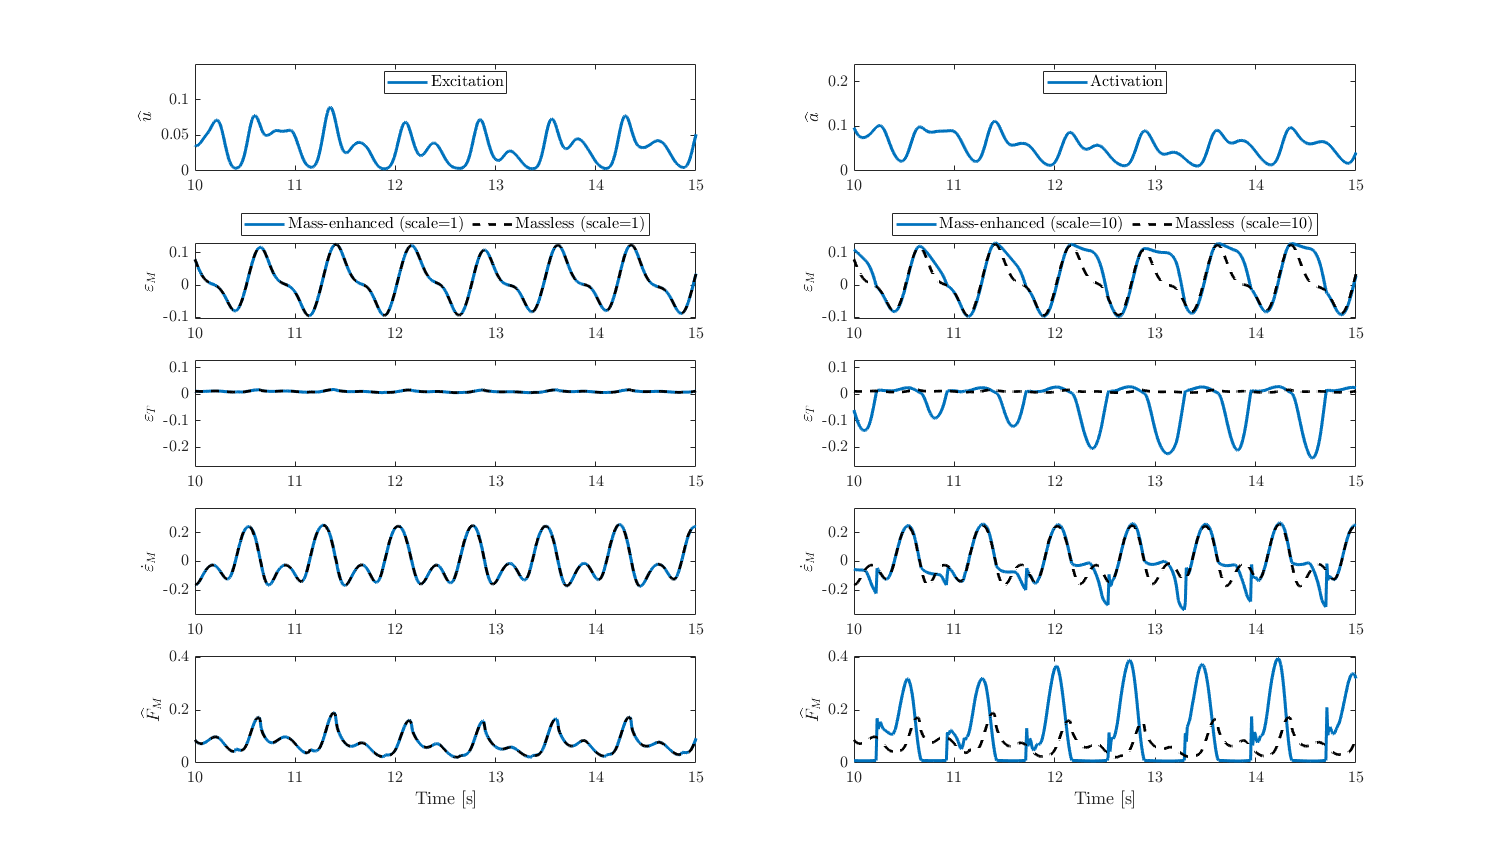
\includegraphics[width=1.25\textwidth]{st-running-strains-strain-rates-forces.png}
    \caption{Predicted dynamics using the massless (dashed black lines) and mass-enhanced (solid blue line) models for the ST muscle during running. From top to bottom, the first row shows the (given) muscle excitation and (computed) activation, then the (computed) muscle strain $\varepsilon_M$, muscle strain rate $\depsilon_M$, tendon strain $\varepsilon_T$, and normalized muscle force $\widehat{F}_M = F_M/F_0$.}
    \label{fig:multibody_traces_ST_running}
\end{figure}

\subsection{Influence of the number of masses in the computation}

The phenomenon in the previous subsection is a strong indication that, in certain scenarios, the number of masses in the model might need to be modified from the standard $N=16$ suggested by Ross et al. \cite{Ross2018-1D}. To view this in more detail, we performed a homogenization study by varying the number of masses from 0 (i.e., a simulation using the massless model) to 128 masses. We portray these results in Figure \ref{fig:multibody-homog-study}. Here, we observe how it is only when using $N=128$ masses that we do not observe any unphysical oscillations. However, simulating 18 seconds of data took about 42 hours of computational time and a significant amount of memory, so this is not a feasible approach for studying multiple muscle-task combinations. 

{\color{blue}In general, we observed that the number of masses needed to fully resolve the traces depended on the scale, task, and muscle in study. This effect can be seen from Figure \ref{fig:multibody_predicted_forces_1_10}B. In particular, for scale $s=10$, the traces for the VM-running and ST-running combination show some spurious oscillations that are not present in the traces for the MG. This also suggests that the problem could be better approached using a one-dimensional \textit{continuum} model (see next chapter), that is, a model derived from an infinitely large number of masses (i.e. $N \to \infty$). This would open the door to the development of efficient numerical solvers using techniques such as the finite element method.}

\begin{figure}
    \centering
    \hspace*{-3.5em}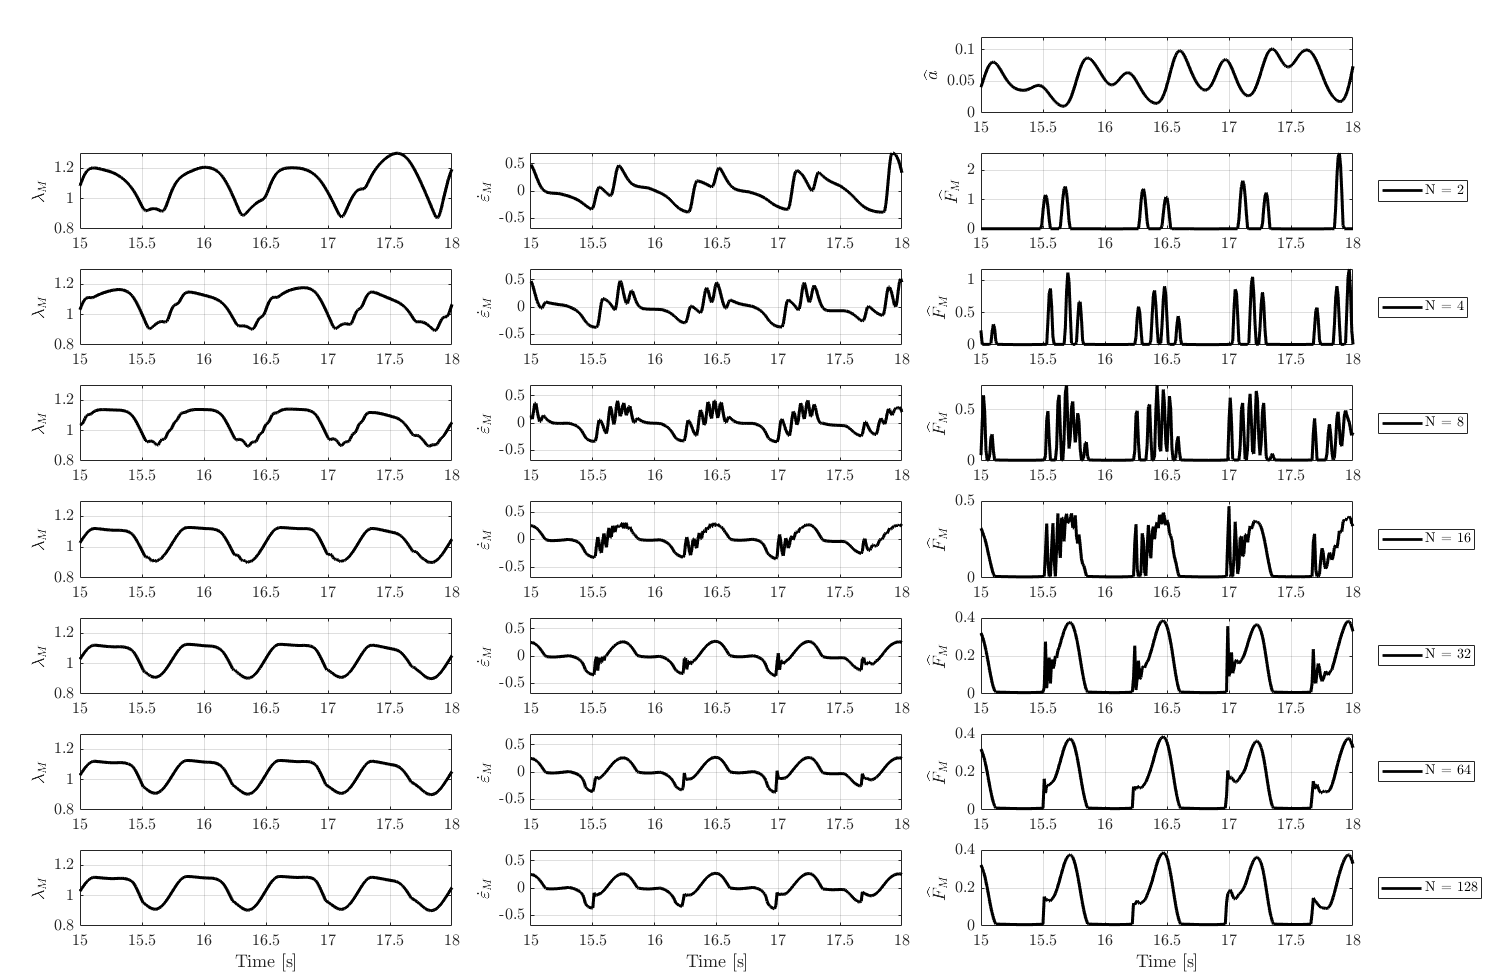
\includegraphics[width=1.2\textwidth]{multibody-homog-study.png}
    \caption{Traces of muscle strains ($\lambda_M$), strain rates ($\depsilon_M$), and (normalized) muscle force $\widehat{F}_M$ as the number of masses vary in the mass-enhanced model: from $N=0$ (second row, i.e. massless model), $N=2$ (third row), up to $N=128$ (last row). For reference we have added the computed activation in the first row.}
    \label{fig:multibody-homog-study}
\end{figure}


\chapter{Dynamical stability and the continuum limit of multibody models}

We now turn our attention to the issue of stability in muscle models. In particular, we refer to a dynamical system (such as the mass-enhanced model \eqref{eq:massenhanced_model}) being \textit{dynamically} stable if small perturbations or deviations from an equilibrium state result in the system eventually remaining near or returning to that equilibrium state over time (see, e.g., \cite{strogratz}). This is in contrast to the concept of \textit{numerical} stability, which is tied to the numerical scheme used to approximate the solution to a dynamical system. We remark that these terms are \textit{not} interchangeable and that the present chapter will focus entirely on the dynamical stability of models such as \eqref{eq:massenhanced_model}.

First, we introduce the context in which multibody models are unstable and the mathematical reasons behind. We present some numerical experiments to visualize the effects of this instability. Next, we propose a simple method to stabilize the system based on previously-validated three-dimensional models. This will require us to explore the continuum limit of the mass-enhanced model, that is, as the number of masses in the system grows infinitely. Finally, we visualize the dynamics on this updated system and the implications when analyzing the mass effects in a one-dimensional context.

%In this chapter, we focus on the \textit{dynamical} stability of the mass-enhanced model introduced in the previous chapter. More precisely, we study the instability of the system \eqref{eq:massenhanced_model} during isomeric contractions along a region of the total FL relationship known as the \textit{descending limb}, a phenomenon known as the \textit{descending limb instability} (DLI). Given that this is only a computational phenomenon and not a physiological one, it is clear that models such as \eqref{eq:massenhanced_model} lack an important feature describing skeletal muscle tissue. 

%First, we describe the DLI and an experiment that replicates it based on the mass-enhanced model introduced in the previous chapter. Next, we show that this model can be viewed as a particular discretization of a one-dimensional \textit{partial} differential equation (PDE). Then, we introduce an additional term to this PDE that can be seen as a passive element not captured by the PEE in Hill's equation \eqref{eq:Hill_force} (that is, the passive force-length relationship $f_P$). Finally, from this PDE, we retrieve a new version of the mass-enhanced model for which we repeat the stability tests that describe the DLI. We will see that this new model is indeed stable at all regions of the total FL relationship.

\section{Background}

The force-length (FL) relationship, which was described for the first time in 1966 for the semitendinosus muscle in frogs \cite{GordonHuxleyJulian1966}, is an important component of Hill-type muscle models. It describes the contractile forces generated by the active and passive elements in a muscle fibre. 

The active force-length curve is a ``bell''-shaped curve that characterizes the actin-myosin interactions formed upon activation. At a sarcomere level, an increasing level of activation leads to a greater overlap between actins and myosins, but only until the sarcomere has reached its optimal length. Beyond this, the overlap between actin and myosin decreases. This reduction means fewer cross-bridges can form, thereby decreasing the ability of the sarcomere to generate active force. Because a muscle fibre can be seen as a bundle of serially-connected sarcomeres, the active force that a muscle fibre generates is assumed to follow this same logic (see Figure \ref{fig:ascending_descending_limbs}A). In turn, the passive force combines the force-generating effects of extracellular components (such as the endomysium, perimysium, epimysium, and sarcolemma) and intracellular components (such as titin) that act to prevent overstretching.

%The active component is generally measured using isometric contractions, that is, the muscle is stretched to a desired length \textit{and then} activated to 100\%. This experiment yields a bell-like curve in which the muscle force increases for increasing muscle lengths below optimal length (i.e. $\lambda_M < 1$), but decreases once the muscle is stretched past optimal length (i.e. $\lambda_M > 1$). The former region is known as the \textit{ascending} limb of the active FL relationship, while the latter is known as the \textit{descending} limb (see Figure \ref{fig:ascending_descending_limbs}A). In turn, the passive force only acts (non-negligibly) for muscle lengths above optimal length, primarily to prevent overstretching.

\begin{figure}
    \centering
    \begin{overpic}[width=\textwidth]{FL_ascending_descending.png}
        \put (4,33) {{\huge \textbf{A}}}
        \put (50,33) {{\huge \textbf{B}}}
    \end{overpic}
    \caption{(A) Active and passive FL relationships. The region $\lambda_M < 1$ corresponds to the ascending limb (in blue) since the curve has a positive slope. In turn, the region $\lambda_M > 1$ corresponds to the descending limb (in ochre) which has a distinctive negative slope. (B) When active and passive forces are added, they form the \textit{total} FL relationship, which typically has a dip region (i.e. a region with negative slope) around $1 < \lambda_M < 1.35$.}
    \label{fig:ascending_descending_limbs}    
\end{figure}

The region on which the active force is increasing (that is, $\lambda_M < 1$) is known as the \textit{ascending} limb, whereas the region where the force is decreasing (that is, $\lambda_M > 1$) is known as the \textit{descending} limb. 
When active and passive forces are combined, the resulting curve may have a ``dip'' region because the passive curve has a slope that is not positive enough to overtake the negative slope of the active curve (see Figure \ref{fig:ascending_descending_limbs}B). This is particularly problematic if the goal is to simulate isometric contractions in this dip region using a multibody model such as the mass-enhanced model \eqref{eq:massenhanced_model}. A small perturbation of the system in this region can generate dynamics that do not reflect the behaviour of skeletal muscle. This phenomenon is known as the \textit{descending limb instability} and has been a subject of discussion for almost 20 years \cite{AllingerEpsteinHerzog1996,YeoEtAl2023NumericalInstability,Zahalak1997}. We remark that this is an instability of \textit{dynamical} type, not numerical (as sometimes is referred to, see \cite{YeoEtAl2023NumericalInstability}). A more precise description of this phenomenon can be made using tools from dynamical systems, which will be the goal of the next section.

\section{Mathematical description of the descending limb instability} \label{sec:dli}

Let us dive into the reasons behind the descending limb instability (DLI) in the context of the mass-enhanced model \eqref{eq:massenhanced_model}. This will be useful to understand what originates this instability and what can be done to remediate it. We begin this section by establishing what an isometric contraction means for our purposes.

\begin{definition}[Isometric contraction] \label{def:isometric_contraction}
    Consider a muscle modelled as a series of one-dimensional elastic elements (i.e. as in the mass-enhanced model). We say that a muscle is contracted \textit{isometrically} if the total muscle length $L_M$ remains constant at all times, independent of the activation level. For the case of a muscle-tendon unit (MTU), we say the MTU is contracted isometrically if the combined length of muscle and tendon remains constant throughout the experiment, 
\end{definition}

The definition above implies that, although the length of the muscle (or an MTU) remains fixed during an isometric contraction, the length of its constitutive elements (i.e., each segment in the mass-enhanced model, or the muscle and tendon lengths in an MTU) may experience individual variations.

\subsection{The model for an isometric contraction}

Consider a muscle modelled as a series of $N$ contractile elements with $N-1$ masses distributed in the same fashion as the mass-enhanced model \eqref{eq:massenhanced_model} (see Figure \ref{fig:model_isometric_contraction}). Moreover, assume that the length is given by $\lambda_M L_M$, where $L_M$ is the optimal muscle length and $\lambda_M$ is a given stretch. Then, the system \eqref{eq:massenhanced_model} now reads:
\begin{subequations} \label{eq:odes_hill_only}
    \begin{align}
        m_1 \ddot{u}_1 &= F_2(\lambda_2, \depsilon_2) - F_1(\lambda_1, \depsilon_1), \\
        m_2 \ddot{u}_2 &= F_3(\lambda_3,\depsilon_3) - F_2(\lambda_2,\depsilon_2), \\
        &\hspace{0.6em} \vdots \notag \\
        m_{N-1} \ddot{u}_{N-1} &= F_N(\lambda_N, \depsilon_N) - F_{N-1}(\lambda_{N-1}, \depsilon_{N-1}).
    \end{align}
\end{subequations}
Here, for $i=1,\dots,N-1$, $u_i$ is the displacement of the $i$-th segment, $m_i = m_{mus} / (N-1)$ with $m_{mus}$ being the mass of the muscle, and the forces $F_i$ are given by Hill's force:
\begin{equation} \label{eq:Hill_force_stability}
    F_i(\lambda_i, \depsilon_i) = F_{Hill}(\lambda_i,\depsilon_i) = F_0 \left\{ F_A(\lambda_i) F_V(\depsilon_i) + F_P(\lambda_i) \right\}.    
\end{equation}
Note that, unlike the expression in \eqref{eq:Hill_force}, we are assuming a fully active muscle (i.e. $a(t) = 1$). As before, the segment stretches $\lambda_i$ are given by:
\begin{subequations} \label{eq:def_stretches_stability}
   \begin{align}
        \lambda_1 &= \dfrac{u_1}{l_s^{opt}} + \lambda_M, \\
        \lambda_i &= \dfrac{u_i-u_{i-1}}{l_s^{opt}} + \lambda_M, \quad i=2,\dots,N-1, \\
        \lambda_N &= \dfrac{-u_{N-1}}{l_s^{opt}} + \lambda_M,
   \end{align}
\end{subequations}
with $l_s^{opt} = L_M / N$, whereas the strain rates $\depsilon_i$ are just:
\begin{equation} \label{eq:def_strain_rates_stability}
    \depsilon_i = \dfrac{1}{\depsilon_0} \dfrac{d\dot\lambda_i}{dt}, \quad i=1,\dots,N.
\end{equation}
We remark that, because we are modelling an isometric contraction, these strain rates will be near zero, and thus the contribution from the FV relationship is negligible since $F_V(0) = 1$. However, we decide to leave this dependence in the definition of Hill's force \eqref{eq:Hill_force_stability} and in the right-hand side of \eqref{eq:odes_hill_only} not only to preserve the structure of the muscle model but also to reuse the computational tools developed in the previous chapter.

\begin{figure}
    \centering
    \begin{tikzpicture}
        \centering
        %\node at (-4.5,1) {\huge \textbf{B}};
        \node[inner sep=0pt] at (0,0)
            {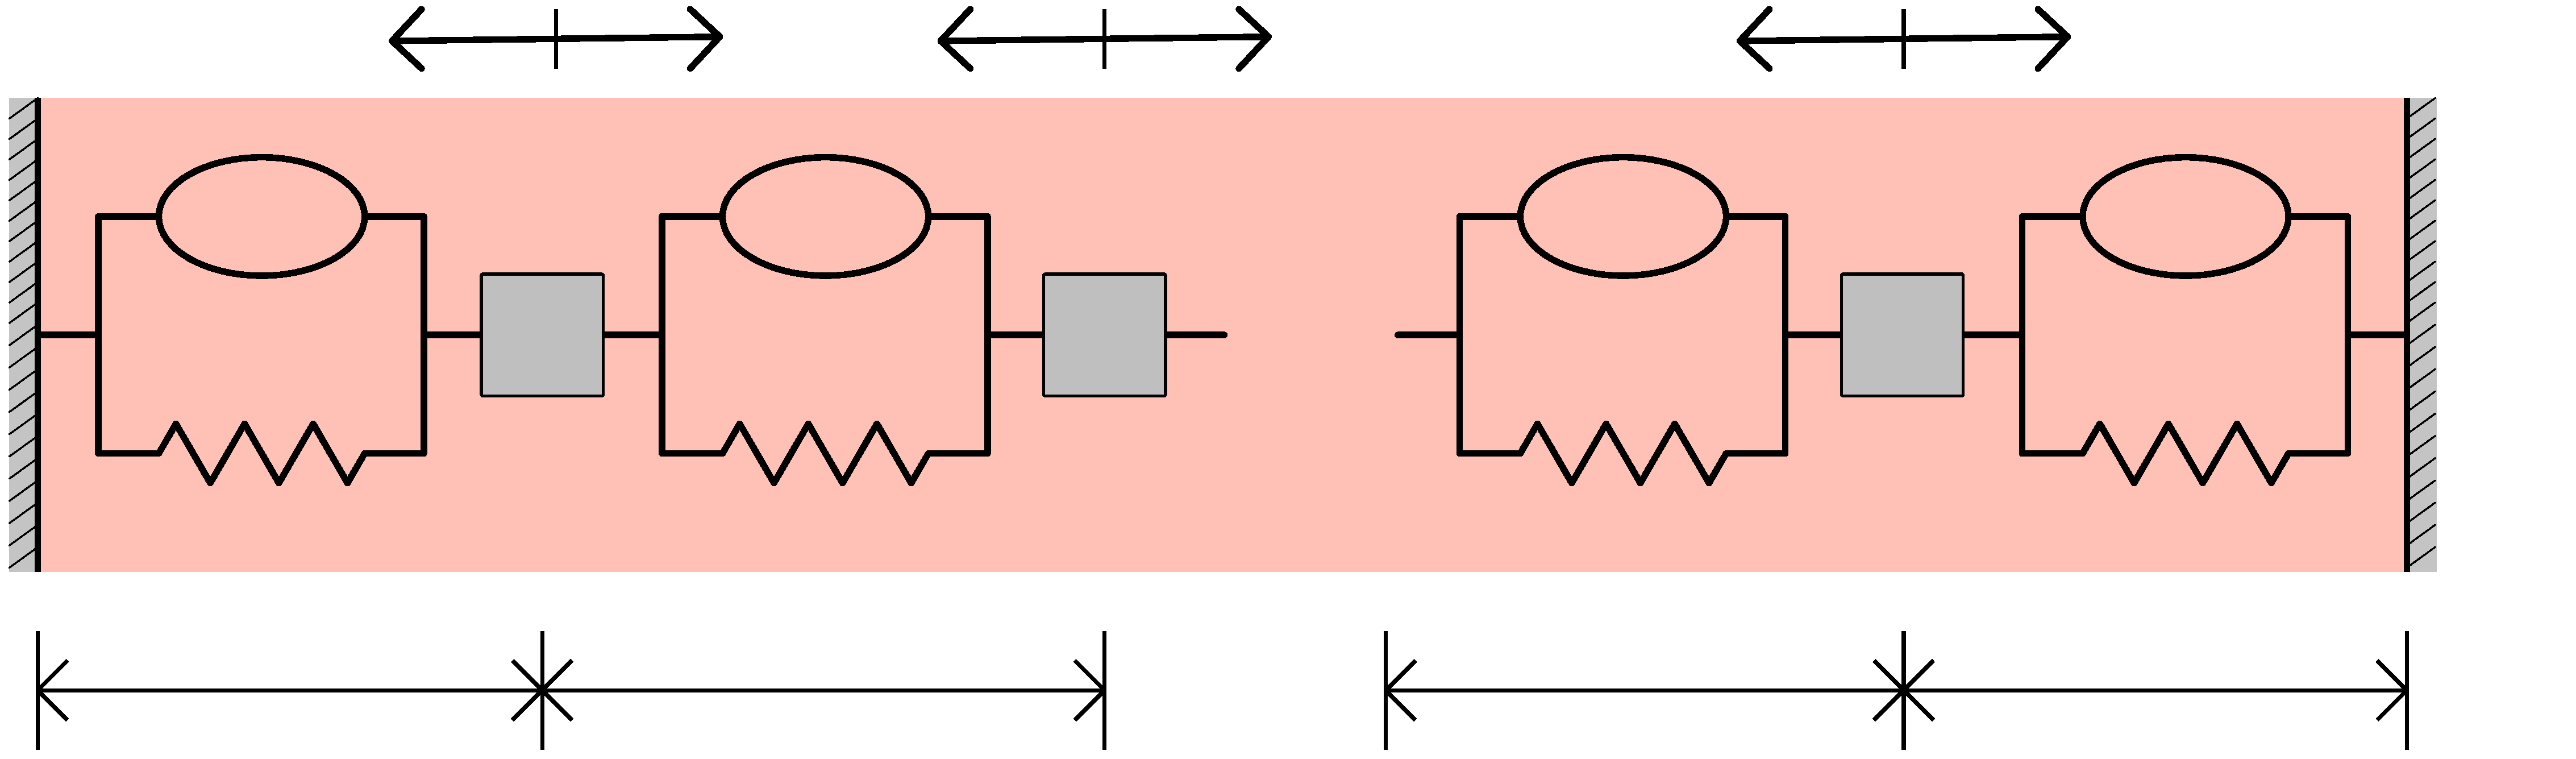
\includegraphics[width=0.525\textwidth]{hill-mass-enhanced-isometric.eps}};
        \node at (-2.31, 0.1) {\tiny $m_1$};
        \node at (-0.56, 0.1) {\tiny $m_2$};
        \node at (1.94, 0.1) {\tiny $m_{\hspace{-0.15em}{N-1}}$};
        \node at (-3.2, 0.5) {\tiny CE$_1$};
        \node at (-3.2, -0.5) {\tiny PEE$_1$};
        \node at (-3.2, -1.26) {\footnotesize $l_1$};
        \node at (-1.45, 0.5) {\tiny CE$_2$};
        \node at (-1.45, -0.5) {\tiny PEE$_2$};
        \node at (-1.45, -1.26) {\footnotesize $l_2$};
        \node at (1.08, 0.15) {\tiny CE$_{{N-1}}$};
        \node at (1.08, -0.5) {\tiny PEE$_{{N-1}}$};
        \node at (2.85, 0.15) {\tiny CE$_{N}$};
        \node at (2.85, -0.5) {\tiny PEE$_{N}$};
        \node at (1.08, -1.26) {\footnotesize $l_{N-1}$};
        \node at (2.85, -1.26) {\footnotesize $l_{N}$};
        \node at (-2.6, 1.45) {\footnotesize $\vec{F}_1$};
        \node at (-2.0, 1.45) {\footnotesize $\vec{F}_2$};
        \node at (-0.9, 1.45) {\footnotesize $\vec{F}_2$};
        \node at (-0.3, 1.45) {\footnotesize $\vec{F}_3$};
        \node at (1.5, 1.45) {\footnotesize $\vec{F}_{N-1}$};
        \node at (2.25, 1.45) {\footnotesize $\vec{F}_N$};
        \node at (0.1,0.14) {\footnotesize $\dots$};
        \node at (-0.1,-1.0) {\footnotesize $\dots$};
    \end{tikzpicture}
    \caption{Mass-enhanced muscle model adapted for an isometric contraction. Here, the sum of all element lengths (i.e. $\sum_{i=1}^N l_i = L_M$) is fixed.}
    \label{fig:model_isometric_contraction}
\end{figure}
 

\subsection{Stability of the zero solution} \label{sec:stability_zero_solution}

%Let us assume that $m_i = m_{mus}/(N-1)$, where $m_{mus}$ is the total muscle mass.
First, we rewrite the system \eqref{eq:odes_hill_only} as a system of first order ODEs, which we can compactly express as:
\begin{equation} \label{eq:odes_hill_only_first_order}
%    \dfrac{d\vec{\xi}}{dt}= \vec{g}\left( \vec{\xi} \, \right),
\dfrac{d}{dt} \begin{pmatrix}
    \vec{u} \\ \vec{v} 
\end{pmatrix} = \dfrac{N-1}{m_{mus}}\begin{bmatrix}
    \*0 & \*I \\ \*0 & \*0
\end{bmatrix} \begin{pmatrix}
    \vec{u} \\ \vec{v} 
\end{pmatrix} + \mathcal{F}(\vec{u}, \vec{v}),
\end{equation}
where $\vec{u} = (u_1, \dots, u_{N-1})^\top$ is the vector of displacements, $\vec{v} = (v_1, \dots, v_{N-1})^\top$ is the vector of velocities (not to be confused with strain rates, see Equation \eqref{eq:def_strain_rates_stability}), and the nonlinear term $\mathcal{F}(\vec{u}, \vec{v})$ is given by
\begin{equation} \label{eq:def_nonlinear_force_term}
    \mathcal{F}(\vec{u}, \vec{v}) = \begin{pmatrix}
        \vec{0} \\ \vec{F}(\vec{u}, \vec{v})
    \end{pmatrix}, \quad 
    \vec{F}(\vec{u},\vec{v}) = \begin{pmatrix}
        F(\lambda_2, \depsilon_2) - F(\lambda_1, \depsilon_1) \\
        \vdots \\
        F(\lambda_N, \depsilon_N) - F(\lambda_{N-1}, \depsilon_{N-1}),
    \end{pmatrix}
\end{equation}
with the force $F$ corresponding to Hill's force with maximal activation ($a=1$), that is
\begin{equation}
    F(\lambda, \depsilon) = F_0 \Big\{ F_A(\lambda)F_V(\depsilon) + F_P(\lambda) \Big\}.
\end{equation}

Notice that the zero solution, that is $(\vec{u}, \vec{v}) = (\vec{0}, \vec{0})$ is an equilibrium point of the system \eqref{eq:odes_hill_only_first_order}. From the definition of the segment stretches $\lambda_i$ in \eqref{eq:def_stretches_stability}, we observe that
\[
u_i = 0 \quad \Rightarrow \quad \lambda_i = \lambda_M, \quad \forall \ i=1,\dots,N-1.
\]
Furthermore, from the definition of the strain rates in \eqref{eq:def_strain_rates_stability} and the velocities in \eqref{eq:odes_hill_only_first_order}, we have
\[
v_i = 0 \quad \Rightarrow \quad \dot{u}_i = 0 \quad \Rightarrow \quad\depsilon_i = \dfrac{1}{\depsilon_0} \dfrac{d}{dt} \left( \dfrac{u_i - u_{i-1}}{l_s^{opt}} \right) = \dfrac{1}{\depsilon_0} \left( \dfrac{\dot{u}_i - \dot{u}_{i-1}}{l_s^{opt}} \right) = 0,
\]
for all $i=1,\dots,N-1$. Therefore, the segment forces that define $\vec{F}$ in \eqref{eq:def_nonlinear_force_term} cancel each other, so the right-hand side of \eqref{eq:odes_hill_only_first_order} vanishes. 

According to the theorem of Hartman-Grobman \cite{HartmanGrobman}, we may linearize \eqref{eq:odes_hill_only_first_order} around $(\vec{0}, \vec{0})$ to analyze the stability of this equilibrium point. Furthermore, because the changes in stretch are will be small relative to the time it takes the system to stabilize, we can assume that $\depsilon_i \approx 0$. Thus, it suffices to analyze the linear system:
\begin{equation}
    \dfrac{d}{dt} \begin{pmatrix}
        \vec{u} \\ \vec{v} 
    \end{pmatrix} = J(\vec{0}, \vec{0}) \begin{pmatrix}
        \vec{u} \\ \vec{v}
    \end{pmatrix},
\end{equation}
where the Jacobian $J(\vec{u}, \vec{v})$, for arbitrary $(\vec{u},\vec{v})$, is given by
\begin{equation}
    J(\vec{u}, \vec{v}) = \begin{bmatrix}
        \*0 & \frac{N-1}{m_{mus}} \*I_{N-1} \\
        \frac{\partial \vec{F}}{\partial \vec{u}} & \*0
    \end{bmatrix},
\end{equation}
with $\*I_{N-1} \in \R^{N-1 \times N-1}$ being the identity matrix and  $\frac{\partial \vec{F}}{\partial \vec{u}}$ the tridiagonal matrix of entries 
\begin{equation}
    \left( \dfrac{\partial \vec{F}}{\partial \vec{u}} \right)_{i,i} = -\frac{1}{l_s^{opt}} \left[ \pder{F}{\lambda}(\lambda_{i+1},0) + \pder{F}{\lambda}(\lambda_i, 0) \right]
\end{equation}
and
\begin{equation}
    \left( \dfrac{\partial \vec{F}}{\partial \vec{u}} \right)_{i+1,i} = \left( \dfrac{\partial \vec{F}}{\partial \vec{u}} \right)_{i,i+1} = 
    \frac{1}{l_s^{opt}} \pder{F}{\lambda}(\lambda_i,0).
\end{equation}
In particular, when $(\vec{u},\vec{v}) = (\vec{0},\vec{0})$, we have 
\begin{equation}
    J(\vec{0}, \vec{0}) = \left[ \begin{array}{cc}
        \*0 & \frac{N-1}{m_{mus}} \*I_{N-1} \\
        \frac{1}{l_s^{opt}}\frac{\partial F}{\partial \lambda}(\lambda_M,0) \, \*D_0 & \*0
    \end{array} \right],
\end{equation}
where $\*D_0 \in \R^{N-1 \times N-1}$ is the matrix
\begin{equation}
    \*D_0 = \left[ \begin{array}{ccccc}
        -2 & 1 & 0 & \cdots & 0 \\
        1 & -2 & 1 & \cdots & 0 \\
          & \ddots & \ddots & \ddots\\
        0 &\cdots & 0 & 1 & -2
    \end{array} \right].
\end{equation}
The latter is a matrix typically found in finite difference schemes for ODEs and PDEs (see, e.g., \cite{Strikwerda}). Its eigenvalues are:
\begin{equation}
    \nu_k = -4 \sin^2 \left( \dfrac{k\pi}{2N} \right), \quad k = 1, \dots, N-1.
\end{equation}
Therefore, to find the eigenvalues $\omega_k$ of $J(\vec{0},\vec{0})$, we may use the following identity:
\[
    \det \left(\omega \*I_{2(N-1)} - J(\vec{0}, \vec{0}) \right) = \det \left(\omega^2 \*I_{N-1} - \dfrac{N-1}{l_s^{opt} m_{mus}} \dfrac{\partial F}{\partial \lambda}(\lambda_M, 0) \*D_0 \right),
\]
which gives rise to two cases, depending on the sign of $\frac{\partial F}{\partial \lambda}(\lambda_M, 0)$.

First, if $\frac{\partial F}{\partial \lambda}(\lambda_M, 0) > 0$ (that is, the muscle is contracted on the \textit{ascending} limb of the FL relationship), then the eigenvalues of the Jacobian are:
\begin{equation}
    \omega_k = \pm 2 \dfrac{N-1}{l_s^{opt} m_{mus}} \frac{\partial F}{\partial \lambda}(\lambda_M, 0) \sin \left( \dfrac{k\pi}{2N} \right) i, \quad k = 1, \dots, N-1,
\end{equation}
with $i=\sqrt{-1}$. Although all the eigenvalues are purely complex, they are distinct, and therefore the system \eqref{eq:odes_hill_only_first_order} is stable according to \cite[Theorem 13.1]{HairerNorsettWanner}. 

In contrast, if $\frac{\partial F}{\partial \lambda}(\lambda_M, 0) < 0$ (that is, the muscle is contracted on the \textit{descending} limb of the FL relationship), then the eigenvalues are purely real:
\begin{equation}
    \omega_k = \pm 2 \dfrac{N-1}{l_s^{opt} m_{mus}} \frac{\partial F}{\partial \lambda}(\lambda_M, 0) \sin \left( \dfrac{k\pi}{2N} \right), \quad k = 1, \dots, N-1.
\end{equation}
Therefore, because of the presence of positive eigenvalues, the system \eqref{eq:odes_hill_only_first_order} is unstable. This is a mathematical characterization of the descending limb instability (DLI).

\subsection{A numerical example} \label{sec:stability_numerical_experiment}

Consider as in \cite{YeoEtAl2023NumericalInstability} a muscle of length $L_M = 0.3$ m with maximum isometric force $F_0 = 525 $ N. Without loss of generality, we set the maximum strain rate to $\depsilon_0 = 5$ s$^{-1}$. We also take $N=17$ masses and an initial condition $u_i = \eta_i$, $\dot{u}_i = 0$, for $i=1,\dots,N-1$, with $\eta_i$ being a random variable drawn from a uniform distribution on $[-0.01, 0.01]$.

To observe the DLI, we perform three isometric contractions in different parts of the FL curve:
\begin{enumerate}
    \item On the ascending limb at $\lambda_M = 0.85$,
    \item On the descending limb at $\lambda_M = 1.15$,
    \item On the descending limb but at a point where the derivative of the total FL curve is positive, say $\lambda_M  = 1.45$.
\end{enumerate}
We show these results in Figure \ref{fig:hill_only_unstable}. Here, we see that when $\lambda_M = 0.85$ or $\lambda_M = 1.45$, we have that $\frac{\partial F}{\partial \lambda}(\lambda_M, 0) > 0$ and therefore the system eventually returns to a static equilibrium where all the segments have the same length. However, when $\lambda_M = 1.15$, we have that $\frac{\partial F}{\partial \lambda}(\lambda_M, 0) < 0$ and a bifurcation is produced: muscle segments diverge to two different lengths that produce the same force.

\begin{figure}
    \centering
    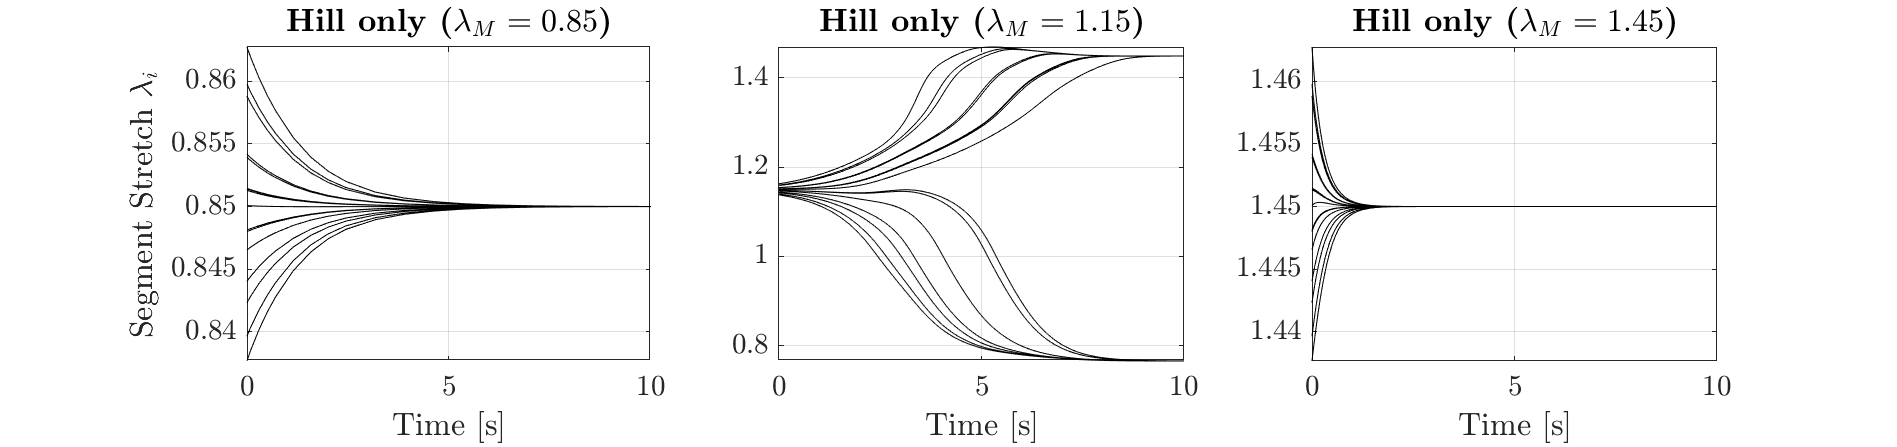
\includegraphics[width=\textwidth]{05_no_bm_unstable.png}
    \caption{Stability of an isometric contraction according to the system of ODEs \eqref{eq:odes_hill_only}. The elements (as well as the muscle) are stretched initially at around 85\% (left), 115\% (middle), and 145\% (right) of the muscle's optimal length. At an initial stretch of 115\%, the descending limb instability causes the segments to bifurcate to two different lengths.}
    \label{fig:hill_only_unstable}
\end{figure}

\section{Stabilizing the model} \label{sec:stabilizing_the_model_ch3}

The model \eqref{eq:odes_hill_only} allows for an arbitrary number of contractile units. Therefore, it is perfectly reasonable to assume a large enough $N$ can reduce each contractile unit into the representation of a sarcomere. In this scenario, the DLI would tell us that sarcomeres may undergo sudden overstretching or ``popping'' when the muscle is isometrically contracted at a length beyond optimal. And while this \textit{is} a physiological phenomenon known as \textit{sarcomere popping} \cite{Morgan1990,MorganProske2004,MorganProske2006}, experiments on single myofibrils show a rather stable behaviour of sarcomeres, i.e. no ``popping'' on the scale of a myofibril \cite{JohnstonJinhaHerzog2016}.

Deriving an accurate, stable, and physiologically-informed muscle model is then an almost Sisyphean task. The properties of skeletal muscle tissue are so heterogeneous that the behaviour of a first-stretched-then-activated muscle fibre (which is how the active force curve is constructed) is completely different compared to one which is first activated and then stretched. At the sarcomere level, this active stretching typically yields FL curves that do not have a dip region, leading to forces that are above the maximum isometric force. This phenomenon is known as \textit{residual force enhancement} (RFE) and, at least mathematically, explains why sarcomeres are stable in both ascending and descending limbs of the active FL curve \cite{JoumaaLeonardHerzog2008}. 

History-dependent effects, such as RFE, are typically attributed to \textit{titin}, the largest protein in the human body and a component of the parallel elastic element in sarcomeres. Upon active stretch, titin binds to actin to increase its stiffness \cite{Nishikawa2020}, with a large enough increase that the total FL curve no longer has a dip region (if it had one), thus \textit{convexifying} the curve. In this way, it is no surprise that muscle models that do include titin as an activation-dependent elastic element are stable \cite{HeidlaufEtAl2016,HeidlaufEtAl2017,LemosEtAl2001,Millard2024,SampaioDeOliveiraUchida2025}. 

RFE has always been observed in single muscle fibres from humans and animals \cite{JoumaaLeonardHerzog2008, Pinnell2019,RassierPavlov2012}. However, RFE may not always be observed \textit{in vivo} at the whole muscle level \cite{Bakenecker2020,Chapman2018,Hinks2024}, yet the contractions are still stable. Could there be components different than titin that bring stability to a muscle fibre?

In mathematical terms, the DLI can be overcome by adding \textit{any} stiff-enough elastic element (not necessarily titin) to Hill's model \eqref{eq:Hill_force_stability}. Therefore, it is also not surprising that three-dimensional models are, more often than not, stable given the addition of a passive, base material contribution \cite{AlmonacidEtAl2022_SIAP_Paper}. Hence, we can draw inspiration from these models to add a hyperelastic component to the system \eqref{eq:odes_hill_only} and show that the resulting model is stable on both limbs of the active FL curve. Given that this is performed at the continuum level, we must first introduce a continuum version of the mass-enhanced model by taking the limit as the number of masses $N \to \infty$.

\subsection{The continuum limit of the mass-enhanced model}

Consider the model \eqref{eq:odes_hill_only} but with an additional mass at the right end that is pulled with a constant force $F_{ext}$. Furthermore, assume that $m_i = m_{mus}/N$ and the muscle is not pre-stretched, i.e. $\lambda_M = 1$. In addition, define $l_s^{opt} = L_{mus}^{opt}/N =: \Delta x$. After some algebraic manipulations, the system \eqref{eq:odes_hill_only} becomes:
\begin{subequations} \label{eq:continuum_model_1}
    \begin{align}
        \dfrac{m_{mus}}{L_{mus}^{opt}} \ddot{u}_1 &= \dfrac{F(\lambda_2, \depsilon_2) - F(\lambda_1, \depsilon_1)}{\Delta x}, \\
        \dfrac{m_{mus}}{L_{mus}^{opt}} \ddot{u}_2 &= \dfrac{F(\lambda_3,\depsilon_3) - F(\lambda_2,\depsilon_2)}{\Delta x}, \\
        &\hspace{0.6em} \vdots \notag \\
        \dfrac{m_{mus}}{L_{mus}^{opt}} \ddot{u}_{N} &= \dfrac{F_{ext} - F(\lambda_{N}, \depsilon_{N})}{\Delta x}.
    \end{align}
\end{subequations}
In particular, the segment stretches $\lambda_i$ and strain rates $\depsilon_i$ now read:
\begin{equation} \label{eq:continuum_model_2}
    \lambda_i = 1 + \dfrac{u_i-u_{i-1}}{\Delta x},
\end{equation}
and
\begin{equation} \label{eq:continuum_model_3}
    \depsilon_i = \dfrac{1}{\depsilon_0} \dfrac{d}{dt} \left( \dfrac{u_i-u_{i-1}}{\Delta x} \right).
\end{equation}

We are interested in studying the behaviour of the system \eqref{eq:continuum_model_1}-\eqref{eq:continuum_model_3} as $N \to \infty$, or equivalently, as $\Delta x \to 0$. This is the \textit{continuum limit}. In this case, equations \eqref{eq:continuum_model_2} and \eqref{eq:continuum_model_3} define the following the quantities:
\begin{equation}
    \lambda(x,t) := \lim_{\Delta x \to 0} \lambda_i = 1 + \pder{u}{x},
\end{equation}
and
\begin{equation}
    \depsilon(x,t) = \lim_{\Delta x \to 0} \depsilon_i = \dfrac{1}{\depsilon_0} \pder{}{t}\left(\pder{u}{x} \right) = \dfrac{1}{\depsilon_0} \pder{\lambda}{t}.
\end{equation}
That is, we have recovered the one-dimensional version of the stretch and strain rate variables that are commonly considered in solid mechanics. Moreover, we can make the following claim with respect to the system \eqref{eq:continuum_model_1}.

\begin{claim} \label{cl:hill_pde}
The system of ODEs \eqref{eq:continuum_model_1} corresponds to a first-order method of lines discretization of the partial differential equation (PDE):
\begin{equation} \label{eq:hill_pde_1}
    \rho_{0,L} \pder{^2 u(x,t)}{t^2}  = \pder{F(\lambda(x,t),\depsilon(x,t))}{x}, \quad 0 < x < L_{mus}^{opt}, \quad 0 < t < \infty,
\end{equation}
subject to boundary conditions
\begin{subequations} \label{eq:hill_pde_2}
    \begin{align}
        u(0,t) &= 0, \\
        F(\lambda(\cdot, t),\depsilon (\cdot, t))\Big|_{x=L_{mus}^{opt}} &= F_{ext}(t), \label{eq:Neumann_F_ext}
    \end{align}
\end{subequations}
and initial conditions
\begin{equation} \label{eq:hill_pde_3}
    u(x,0) = \pder{u}{t} = 0.
\end{equation}
Here, $F$ corresponds to Hill's force defined in \eqref{eq:Hill_force_stability} and $\rho_{0,L} := m_{mus}/L_{mus}^{opt}$ is a linear density.
\end{claim}

Note that the Neumann condition \eqref{eq:Neumann_F_ext} to a nonlinear type of boundary condition depending on $\frac{\partial u}{\partial x}$. Thus, the problem \eqref{eq:hill_pde_1}-\eqref{eq:hill_pde_3} is at least well-defined. Whether it is \textit{well-posed} (that is, given a smooth $F_{ext}$, the problem has a unique regular solution depending continuously on $F_{ext}$) is a different story and will not be discussed here. As it is known, this can only be done in limited scenarios (for instance, when $F$ is linear, see \cite{TruesdellNoll2004}), so a general result cannot be stated for arbitrary $F$ and $F_{ext}$.

\begin{proof}
    Consider a discretization $\{x_0, x_1, \dots, x_N\}$ with constant spacing $\Delta x := L_{mus}^{opt}/N$ of the interval $[0,L_{mus}^{opt}]$ where $x_0 = 0$ and $x_N = L_{mus}^{opt}$, then, define $u_i := u(x_i,t)$ for $t \geq 0$, $i=1,\dots,N$. Furthermore, consider a backwards first-order formula for the stretch and strain rates, that is,
    \[
        \lambda_i = \lambda(x_i,t) = 1 + \dfrac{u_i-u_{i-1}}{\Delta x},
    \]
    and
    \[
        \depsilon_i = \depsilon(x_i, t) = \dfrac{1}{\depsilon_0}\dfrac{d\lambda_i}{dt}.
    \]
    These are precisely \eqref{eq:continuum_model_2} and \eqref{eq:continuum_model_3}. Now, to discretize the gradient on the right-hand side of \eqref{eq:hill_pde_1}, consider a forwards first-order difference:
    \[
        \rho_{0,L} \dfrac{d^2 u_i}{dt^2} = \dfrac{F(\lambda_{i+1},\depsilon_{i+1}) - F(\lambda_i, \depsilon_i)}{\Delta x}, \quad i =1, \dots, N.
    \]
    Given that there is not an $x_{N+1}$ mass, the force required at this ``ghost'' node can be taken precisely as $F_{ext}$ according to the boundary condition \eqref{eq:Neumann_F_ext}. Hence, the previous expression is just \eqref{eq:continuum_model_1}.
\end{proof}

\subsection{Convexifying the FL relationship}

Let us introduce a base material component to Hill's force \eqref{eq:Hill_force_stability} assuming that it behaves as Neo-Hookean material:
\begin{equation} \label{eq:force_neohookean}
    F_{NH}(\lambda) = \left\{
        \begin{aligned}
            &F_0 \dfrac{\kappa}{\sigma_0} \left( \widehat{\mathcal{L}}_{\mu} \lambda +  \dfrac{\widehat{\mathcal{L}}_{\lambda} \log(\lambda) - \widehat{\mathcal{L}}_\mu}{\lambda}\right), \quad &\lambda \geq 1, \\
            &0, \quad &\text{otherwise}.
        \end{aligned}
    \right.
\end{equation}
Here, $\kappa$ is the bulk modulus of muscle, $\sigma_0$ is the maximum isometric stress, and the (non-dimensional) Lam\'{e} parameters are given by
\begin{equation}
    \widehat{\mathcal{L}}_{\lambda} = \dfrac{\nu}{(1-\nu)(1-2\nu)}, \quad \widehat{\mathcal{L}}_{\mu} = \dfrac{1}{2(1+\nu)},
\end{equation}
with $\nu$ being the Poisson's ratio of muscle tissue, which can be set to $\nu = 0.499$ owing to the (near-)incompressibility of muscle \cite{Kuthe2016}.

In principle, the PDE \eqref{eq:hill_pde_1} can be seen as a model for the one-dimensional deformation of a muscle fibre in which every point inside is subjected to Hill's force. Therefore, if we think of a fibre as a bundle of myofibrils, then we can consider the components that are in between to be part of the base material of a fibre. These components include (but are not limited to) the sarcoplasmic reticulum and the T-tubules. In this way, we consider the following expression for the muscle force in \eqref{eq:hill_pde_1}:
\begin{equation} \label{eq:force_hill_plus_bm}
    F(\lambda, \depsilon) = (1-\chi_{BM}) F_{Hill}(\lambda, \depsilon) + \chi_{BM} F_{NH}(\lambda),
\end{equation}
where $\chi_{BM}$ denotes the fraction of base material that could be present in a muscle fibre. Thus, the more base material we introduce in the model, the more we can convexify the FL curve. Luckily, $\chi_{BM}$ does not have to be large to bring stability to the system, as we will see in the experiment below.

\subsection{A stabilized mass-enhanced muscle model} \label{sec:stabilized_muscle_model_1d}

Following the result in Claim \ref{cl:hill_pde}, we can write a stabilized version of \eqref{eq:odes_hill_only} using the force expression \eqref{eq:force_hill_plus_bm}:
\begin{multline} \label{eq:odes_hill_stabilized}
    \quad m_{i-1} \ddot{u}_{i-1} =
    (1-\chi_{BM})\left[ F_{Hill}(\lambda_i, \depsilon_i) - F_{Hill}(\lambda_{i-1}, \depsilon_{i-1}) \right] \\ 
    + \chi_{BM}\left[ F_{BM}(\lambda_i) - F_{BM}(\lambda_{i-1}) \right], \quad i = 1,\dots,N-1, \quad 
\end{multline}
with the stretches $\lambda_i$ and strain rates $\depsilon_i$ as in \eqref{eq:def_stretches_stability} and \eqref{eq:def_strain_rates_stability}, respectively. Then, we can repeat the experiment from Section \ref{sec:stability_zero_solution} to test the stability of the zero solution. In particular, we take in equation \eqref{eq:force_hill_plus_bm} a bulk modulus $\kappa = 10^6 \ \text{Pa}$ and a maximum isometric stress $\sigma_0 = 200 \ \text{kPa}$ \cite{AlmonacidEtAl2022_SIAP_Paper}. Furthermore, we consider $\chi_{BM} = 0.0015$, that is, we assume that 99.85\% of the force that a muscle fibre produces is due to Hill's force and 0.15\% from a base material contribution. 

\begin{figure}
    \centering
    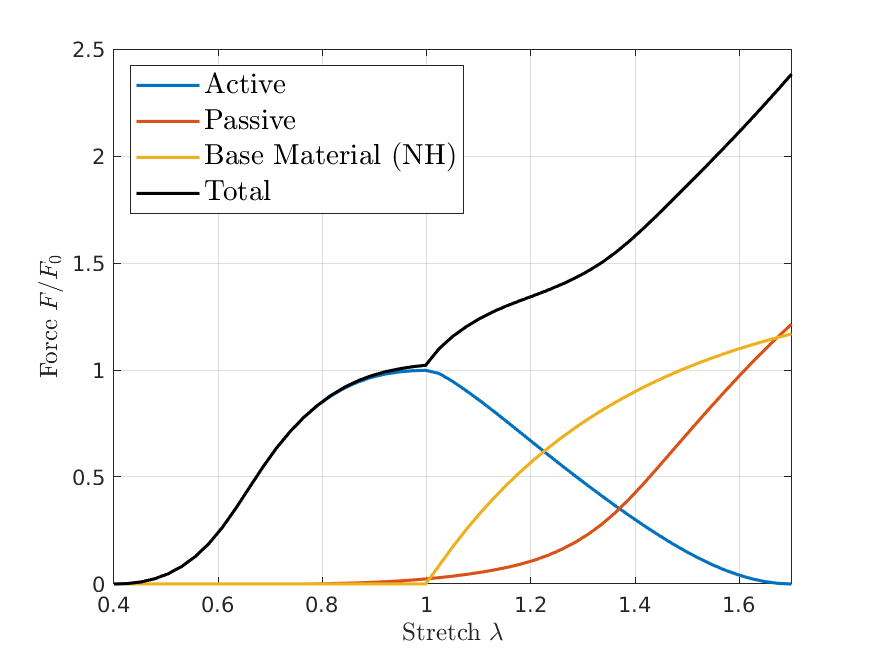
\includegraphics[width=0.75\textwidth]{03_forces_with_bm.png}
    \caption{Forces in the stabilized model \eqref{eq:odes_hill_stabilized}. When the base material component (yellow) is added to the active (blue) and passive (red) forces, the total force (black) is a monotonically increasing function.}
    \label{fig:forces_stabilized}
\end{figure}

First, we portray the resulting forces in Figure \ref{fig:forces_stabilized} where the total force \eqref{eq:force_hill_plus_bm} shows RFE for muscle lengths above optimal (i.e. $\lambda_M > 1$). Then, in Figure \ref{fig:hill_plus_nh_stable} we show the results for the same three isometric contractions as in Section \ref{sec:stability_numerical_experiment} which show (1): no difference for $\lambda_0 = 0.85$ since the Neo-Hookean term does not act for stretches below 1, (2): stabilization on the descending limb of the active FL curve, shown in the figure for $\lambda_0 = 1.15$, and (3): rapid stabilization due to a stiffer passive element. Therefore, it is clear that the base material component has a stabilizing effect in isometric contractions. 

\begin{figure}
    \centering
    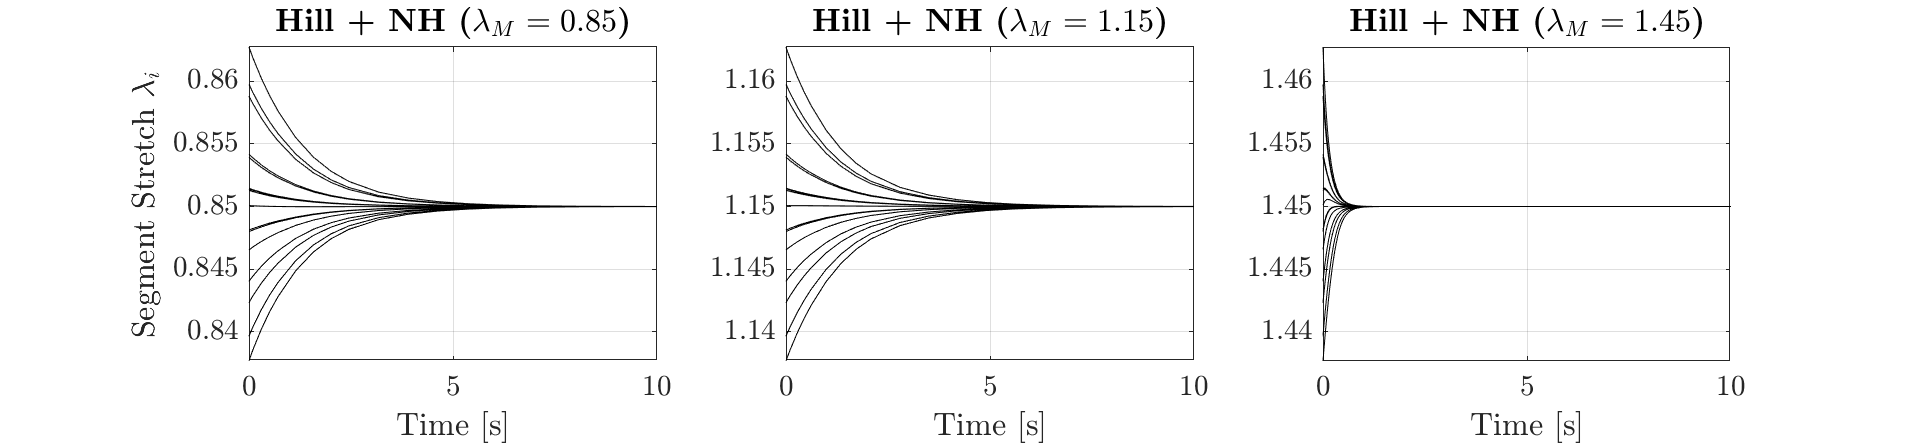
\includegraphics[width=\textwidth]{06_with_bm_stable.png}
    \caption{Stability of an isometric contraction according to the system of ODEs \eqref{eq:odes_hill_stabilized}. As before, the elements (as well as the muscle) are stretched initially at around 85\% (left), 115\% (middle), and 145\% (right) of the muscle's optimal length. In all cases, the contractions are stable since the derivative of the total force (made of active, passive, and base material components) is always positive.}
    \label{fig:hill_plus_nh_stable}
\end{figure}

\section{Nondimensionalization of the continuum system and the influence of mass}

The elastic model \eqref{eq:hill_pde_1} with the force $F$ given by \eqref{eq:force_hill_plus_bm} can be used to explain the mass effects discussed in Chapter \ref{ch:mass_enhanced_model} in a succinct way. First, let
\begin{equation}
    \widehat{F}_{Hill} = \dfrac{F_{Hill}}{F_0}, \quad \widehat{F}_{NH} = \dfrac{F_{NH}}{F_0},
\end{equation}
denote the nondimensional versions of the Hill and Neo-Hookean force terms. Moreover, consider the following nondimensional variants of the  displacement, space, and time variables:
\begin{equation}
    \widehat{u} = \dfrac{u}{L_{mus}^{opt}}, \quad \widehat{x} = \dfrac{x}{L_{mus}^{opt}}, \quad \widehat{t} = \dfrac{t}{1/\depsilon_0}.
\end{equation}
Plugging these quantities into \eqref{eq:hill_pde_1} we obtain:
\begin{equation} \label{eq:nondim_1}
    \dfrac{\rho_{0,L} (L_{mus}^{opt})^2 \depsilon_0^2}{F_0} \, \pder{^2 \widehat{u}}{\widehat{t}^2} = (1-\chi_{BM}) \widehat{F}_{Hill} + \chi_{BM} \dfrac{\kappa}{\sigma_0} \widehat{F}_{BM}.
\end{equation}
All terms in the previous equation are nondimensional, but we can further rearrange the terms in the left-hand side to obtain a more physically meaningful number. 

Recall that $\rho_{0,L}$ is a \textit{linear} density (it has units of $\text{kg} \ \text{m}^{-1}$). We can convert this quantity into the more common \textit{volumetric} density $\rho_0$ through the cross-sectional area (CSA) of a muscle fibre, that is,
\begin{equation}
    \rho_{0,L} = \rho_0 \cdot CSA.
\end{equation}
Moreover, because the maximum isometric force $F_0$ can be written in terms of the maximum isometric stress as $F_0 = \sigma_0 \cdot CSA$, the number on the left-hand side of \eqref{eq:nondim_1} can be written as
\begin{equation}
    \dfrac{\rho_0 (L_{mus}^{opt})^2 \depsilon_0^2}{F_0} = \dfrac{\rho_0 (L_{mus}^{opt})^2 \depsilon_0}{\sigma_0 / \depsilon_0}.
\end{equation}
The nondimensional number in the previous expression can be viewed as a ratio between inertial forces (due to mass) and viscous forces. As such, we call this number the \textit{musculoskeletal Reynolds number} ($\text{Re}_{MSK}$), akin to the Reynolds number commonly found in fluid dynamics. In this way, we can rewrite \eqref{eq:nondim_1} as:
\begin{equation}
    \text{Re}_{MSK} \pder{^2 \widehat{u}}{\widehat{t}^2} = (1-\chi_{BM}) \widehat{F}_{Hill} + \chi_{BM} \dfrac{\kappa}{\sigma_0} \widehat{F}_{BM}.
\end{equation}

\begin{table}
    \centering
    \begin{tabular}{|c|c|c|} \hline
        $s$ & $\depsilon_0$ [s$^{-1}$] & $\text{Re}_{MSK}$ \\\hline
        1 & 5 & $1.1925 \cdot 10^{-5}$ \\\hline
        1 & 10 & $4.77 \cdot 10^{-5}$ \\\hline
        10 & 5 & $1.1925 \cdot 10^{-3}$  \\\hline
        10 & 10 & $4.77 \cdot 10^{-3}$  \\\hline
    \end{tabular}
    \caption{Variation in the musculoskeletal Reynolds number $\text{Re}_{MSK}$ when a scaling factor $s$ is introduced for two different maximum (unloaded) strain rates (5 $\text{s}^{-1}$ and 10 $\text{s}^{-1}$). Here, $\rho_0 = 1.060 \text{ kg} \ \text{m}^{-3}$, $\sigma_0 = 200 \ \text{kPa}$, $L_{mus}^{opt} = 0.3 \ \text{m}$.}
    \label{tab:re_msk}
\end{table}

Therefore, if the length of the muscle scales by a factor $s$, the rescaled musculoskeletal Reynolds number becomes:
\begin{equation}
    \text{Re}_{MSK} = s^2 \, \dfrac{\rho_0 (L_{mus}^{opt})^2 \depsilon_0}{\sigma_0 / \depsilon_0}.
\end{equation}
This explains why one can expect, in this one-dimensional context, that mass effects are larger for larger scales, longer muscles (such as the semitendinosus), and muscles that contain a higher proportion of faster fibres (i.e., larger $\depsilon_0$). See Table \ref{tab:re_msk} for some values of this nondimensional number. 


\chapter{First order is enough: time discretization alternatives for dynamic Neo-Hookean deformation} \label{ch:neohookean}

%Newmark methods, Rothe's vs. method of lines comparisons. Stiff solvers is (one of) the key mathematical concepts here.
%Github repository: one-dimensional-elasticity

%\medskip

As a prelude to the development of computational tools for the study of dynamic 3D skeletal muscle deformation, we now face the task of finding an appropriate time stepping scheme for this problem. This is an effort to extend the developments of Rahemi \cite{Hadi} and Dominguez \cite{Seba} regarding quasi-static models.  
To accomplish this, we study the performance of different time stepping schemes, from methods used in engineering finite element analysis to Matlab's built-in solvers. 
%However, instead of applying these methods directly to the muscle problem, we study them in the context of one-dimensional Neo-Hookean deformation. This provides us with a simple (yet representative) model to efficiently test different numerical algorithms.
However, because the complexity of the full 3D nonlinear model obscures the main details of the numerical algorithms in use, we therefore focus on applying these methods to a simpler (yet representative) model of one-dimensional Neo-Hookean deformation.

First, we discuss time stepping methods that are commonly used in dynamic analysis of structures, as well as their advantages and disadvantages. Next, we state a model problem in 1D and present some of these methods in two different contexts, depending on which variable in the continuous problem is discretized first: time or space. This is a particularly important consideration for nonlinear problems with (potentially) nonsmooth boundary conditions. Then, we present convergence studies for a linear problem. We then perform numerical experiments of Neo-Hookean deformation in order to compare. In addition to classic time stepping methods used in engineering, we also study an implicit-explicit (IMEX) method and several of Matlab's built-in solvers for systems of ODEs. We finish the chapter with a discussion on the obtained results and what this means for the development of a 3D \textit{dynamic} finite element code for skeletal muscle tissue.

\section{Background}

We start with two discussions that will, hopefully, help the reader understand our choices and results for this chapter: what type of time stepping should we choose and what variable (space or time) should be discretized first.

\subsection{Time stepping schemes in engineering elastodynamics}

The discretization of elastodynamic models is a well established research area in engineering. Tried-and-tested techniques are widely available in modern, commonly used finite element analysis software, such as Ansys Mechanical, Ansys LS-DYNA, COMSOL, and Abaqus. In particular, for linear elastodynamics, well-known time stepping schemes include Newmark-$\beta$ schemes \cite{Newmark}, Wilson-$\theta$ schemes \cite{Wilson}, HHT-$\alpha$ schemes \cite{HHTalpha}, WBZ-$\alpha$ schemes \cite{WBZ}, HP-$\theta_1$ methods \cite{HPtheta}, and more recently, structure-dependent schemes (i.e. numerical methods whose parameters depend on the material properties of the structure) such as those by Chang \cite{ChangSD}. In general, studies in mechanical engineering will claim that a good time stepping scheme for the linear problem must have the following characteristics (see, e.g. \cite{HughesBook, KadapaDettmerPeric2017, RossiEtAl2014}):
\begin{enumerate}
    \item Unconditional stability,
    \item Second-order accuracy,
    \item Being single-step, that is, only one set of implicit equations needs to be solved per time step and the only information needed to do this is from the immediately previous time step,
    \item Controllable numerical dissipation in the higher modes,
    \item Self-starting,
    \item Should not \textit{overshoot} the solution.
\end{enumerate}

\textit{Overshooting} is a phenomenon in which the numerical method ``overestimates'' the solution in the first steps due to the excitation of high-frequency modes (see Figure \ref{fig:overshoot}). This is commonly observed in stiff problems where either non-zero or non-smooth boundary conditions are used. Moreover, all the time schemes mentioned at the beginning of this section, are prone to suffer this problem \cite{MaxamTamma2022}. This means that overshooting is, albeit undesirable, a potentially manageable nuisance. %In the worst case scenario, the numerical algorithm will not be able to damp these oscillations


\begin{figure}
    \centering
    \hspace*{-4em}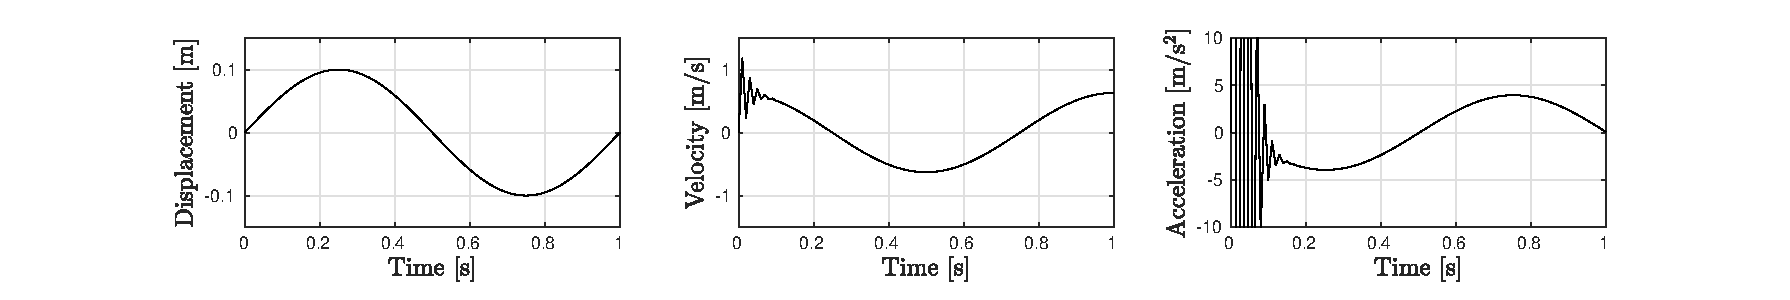
\includegraphics[width=1.19\textwidth]{figs/overshooting.eps}
    \caption{Example of overshooting in the velocity variable, which causes even higher oscillations in the acceleration.}
    \label{fig:overshoot}
\end{figure}

While numerical methods such as Newmark's or HHT-$\alpha$ do verify characteristics 1-6 above in the context of linear problems, they may not for nonlinear problems. Consider the nonlinear second order ODE:
\[
    \ddot{y} = \varphi(y,\dot{y}) \quad \text{in } (0,\infty),
\]
where $\varphi:\R \times \R \to \R$ is smooth function. If an implicit method is used to discretize this equation, then at each time step, the nonlinear problem must be linearized (using strategies such as Newton's method). Furthermore, if iterative solvers are used to solve the (discretized) linear problem, then multiple linear systems are solved at each Newton iteration, and multiple Newton iterations are needed for each time step. Therefore, second-order accuracy might not be achieved, or if it does, the numerical methods might still exhibit overshooting and oscillations beyond the high-frequency regime \cite{ErlicherBonaventuraBursi2002}.

%In general, numerical methods for nonlinear elastodynamics continues to be an active research area (see, e.g. \cite{ChenEtAl2017Fabrication,JanzBetschFranke2019,LiEtAl2020LargeDefornationDynamics,PellecchiaCesarano2021Hysteretic} and the references therein).

\subsection{Time or space first? Rothe's method versus method of lines}

When it comes to numerical methods for spatio-temporal problems, at least two approaches arise depending on the order in which the variables (space and time) are discretized.

One alternative is to discretize the time variable first while keeping the space variable continuous. This is referred to as \textit{Rothe's method} \cite{Rothe1930}. For second order parabolic and hyperbolic systems (the latter being the case for elastodynamics), this means that, at each time step, we are bound to solve an elliptic PDE in the space variable. For nonlinear PDEs, the linearization can be performed at a continuous level using, for instance, G\^{a}teaux derivatives. One of the advantages of this method is that, in the context of finite element methods, updates to the mesh can easily be performed since they do not alter the variational formulation of the elliptic problem. However, one major disadvantage is that it is harder to test different time stepping strategies since they involve modifying the structure of the variational formulation itself, which may induce significant modifications to the computational solvers. We will see these differences throughout Sections \ref{sec:a_firt_order_time_stepping_scheme} to \ref{sec:hht_alpha_method}.

A different approach is to discretize the space variable first, then the time variable. This leads to the \textit{method of lines (MOL)} \cite{LeVequeBook} and it is how Newmark-type methods are introduced in the engineering literature \cite{HughesBook}. In this case, the parabolic or hyperbolic PDE is transformed into a system of ODEs. This is one of the major advantages of the MOL since it is relatively easy to test multiple time stepping schemes implemented as ODE solvers. However, this also means that the spatial mesh is fixed at all times, which is not amenable to a posteriori mesh refinements (especially at each time step).

%\subsection{Refactor or rewrite the code?}

%Aside from a mathematical choice, there is also a software engineering choice to be made. First, the development of a software to 

%\clearpage

%Based on these differences, and specially for nonlinear problems, the choice of Rothe's method or MOL can lead to completely different computational implementations, which is something that we have to take into account in this project, given the complexity of the computational tools\footnote{The original ``muscle code'' developed by Dominguez Rivera in \cite{Seba} consists of a single C++ file with around 10,000}. As we mentioned at the beginning of this chapter, the main goal is to find an appropriate time stepping scheme for the dynamic model of skeletal muscle deformation. The model (which will be the focus of Part II of this thesis) will consist of a three-field formulation very similar to that of Rahemi \cite{Hadi} and Dominguez Rivera \cite{Seba}. In particular, Dominguez Rivera developed a code which implements Rothe's method for the muscle model with a first order  

%Furthermore, we would like to develop our code by extending the work of Dominguez Rivera \cite{Seba}, while improving its efficiency and  

%Therefore, we begin this search having already a computational implementation of a convergent numerical scheme based on Rothe's method and a first order time discretization \cite{Paper1_WakelingEtAl2020}, which we would like to resue. Unfortunately, this particular discretization only works for quasi-static problems (e.g. \cite{Paper2_RyanEtAl2020}), and problems involving passive muscle \cite{KonnoEtAl2022_CP} or muscles with low levels of activation \cite{Cassidy}.

%\clearpage

\section{Model problem for nonlinear elasticity}

Consider a one-dimensional solid (which we may refer to as a ``rod'') of linear density $\rho_{0,L}$ and cross-sectional area $A_0$ that occupies the region $\Omega = [0,L]$. Furthermore, let $u = u(x,t)$ denote the displacement of a point $x$ at time $t$. We consider the following model for the deformation of this rod subject to a prescribed displacement $g = g(t)$ at one of its ends:
\begin{subequations} \label{eq:elasticity_1d}
    \begin{gather}
        \label{eq:elasticity_1d_1}\rho_0 u_{tt} = P_x \quad \text{in }\Omega \times (0,\infty), \\
	    u(x,0) = 0, \quad u_t(x,0) = 0 \quad \text{in } \Omega \times \{t=0\} \\
	    u(0,t) = 0, \quad u(L,t) = g(t) \quad \text{in } (0,\infty).
    \end{gather}
\end{subequations}
Here, $\rho_0 = \rho_{0,L} / A_0$ is a volumetric density and $P = P(\lambda)$ is a constitutive equation for the stress of the material depending on the stretch $\lambda := u_x + 1$. The equation above is very similar to \eqref{eq:hill_pde_1} but with a stress $P$ instead of a force $F$ to match the dimensions of the left-hand side of \eqref{eq:elasticity_1d_1}. 

\section{A first order time stepping scheme} \label{sec:a_firt_order_time_stepping_scheme}

Let us consider a first order scheme inspired by previous works on skeletal muscle modelling (e.g. \cite{Seba,Paper1_WakelingEtAl2020}). To keep the focus on the time discretization, all methods will feature a spatial discretization based on second-order Lagrange finite elements.

\subsection{Rothe's method and finite element formulation} \label{sec:rothe_first_order}

First, we convert the PDE \eqref{eq:elasticity_1d_1} into a system of first order PDEs. Then, we discretize the time derivatives using a first-order backwards formula. This yields the following semi-discrete problem for $n \geq 0$:
\begin{subequations} \label{eq:rothe_first_order}
    \begin{gather}
        \label{eq:disc_u} \frac{u^{n+1}-u^n}{\Delta t} = v^{n+1}, \\
	    \label{eq:disc_v} \rho_0 \left( \frac{v^{n+1}-v^n}{\Delta t} \right) = 
        P(\lambda^{n+1})_x,
    \end{gather}
\end{subequations}
where the stretch $\lambda^{n+1} = \partial_x u^{n+1} + 1$. Combining these two equations into a single one for $u^{n+1}$ yields:
\begin{equation} \label{eq:rothe_first_order_combined}
	\rho_0 u^{n+1} - \Delta t^2 P(\lambda^{n+1})_x = \rho_0 (u^n + \Delta t v^n), \quad n \geq 0.
\end{equation}
Then, we take steps to discretize the spatial variable as specified at the beginning of this section. Multiplying \eqref{eq:rothe_first_order_combined} by a test function $w \in H_0^1(\Omega)$ and integrating by part we obtain the nonlinear variational formulation: find $u^{n+1} \in  H^1(\Omega)$ such that $u^{n+1}(0) = 0$, $u^{n+1}(L) = g(t^{n+1})$, and
\begin{equation} \label{eq:rothe_first_order_VF}
	R(u^{n+1}, w) = 0 \quad \forall \ w \in H_0^1(\Omega),
\end{equation}
where $R:H^1(\Omega) \times H_0^1(\Omega) \to \R$ is the functional defined by
\begin{equation}
    R(u^{n+1},w) := \rho_0 \int_0^L u^{n+1} w + \Delta t^2 \int_0^L P(\lambda^{n+1}) w_x - \rho_0 \int_0^L (u^n + \Delta t v^n) w.
\end{equation}

\subsubsection*{Linearization of the semi-discrete problem}

We solve the nonlinear problem \eqref{eq:rothe_first_order_VF} using Newton's method. Suppose $u^n \approx u(x, t^n)$. Given $u_0^{n+1} = u^n$, the $k$-th iteration reads: find increments $\delta u_k^{n+1}$ such that
\begin{equation} \label{eq:rothe_first_order_lin_1}
    \mathcal{D}R[u_k^{n+1}](\delta u_k^{n+1}, w) = - R(u_k^{n+1}, w) \quad \forall \ w \in H_0^1(\Omega),
\end{equation}
where $\mathcal{D}R$ is the Gâteaux derivative of $R$ and can be computed as:
\begin{equation}
    \mathcal{D}R[u](\delta u,w) = \lim_{\epsilon \to 0} \dfrac{d}{d\epsilon} R(u + \epsilon \delta u, w).
\end{equation}
Therefore, the linear problem \eqref{eq:rothe_first_order_lin_1} becomes: find Newton increments $\delta u_k^{n+1} \in H^1(\Omega)$ such that $du_0^{n+1} = 0$ on $x=0$, $du_0^{n+1} = g(t^{n+1}) - g(t^{n})$ on $x=L$, $\delta u_k^{n+1} = 0$ on $x=0,L$ for k > 0, and:
\begin{multline} \label{eq:rothe_first_order_lin_2}
	\rho_0 \int_0^L \delta u_k^{n+1} \, w + \Delta t^2 \int_0^L \der{P}{\lambda}(\lambda_k^{n+1}) \der{(\delta u_k^{n+1})}{x} \der{w}{x} = \\
	-\rho_0 \int_0^L u_k^{n+1} w - \Delta t^2 \int_0^L P(\lambda_k^{n+1}) \der{w}{x} + \rho_0 \int_0^L (u^n+\Delta t v^n) w,
\end{multline}
for any $w \in H_0^1(\Omega)$, where the stretch for the current Newton iteration is $\lambda_k^{n+1} = \partial_x u_k^{n+1} + 1$. Note that, unlike the nonlinear formulation \eqref{eq:rothe_first_order_VF}, for $k\geq 1$, the linear formulation \eqref{eq:rothe_first_order_lin_2} is symmetric (i.e., test and trial spaces are the same).

The linear problem \eqref{eq:rothe_first_order_lin_2} is solved for each $k \geq 0$ and the displacement is updated as $u_{k+1}^{n+1} = u_k^{n+1} + \delta u_k^{n+1}$ until the following convergence criterion is satisfied:
\begin{equation} \label{eq:convergence_crit_1d}
    \| \delta u_k^{n+1} \| \leq tol_u \quad \text{and} \quad \| R(u_k^{n+1}) \| \leq tol_R,
\end{equation}
where $\|\cdot\|$ is a user-defined discrete norm (e.g. the Euclidean norm) arising from the discretized versions (see below) of the Newton update $\delta u_k^{n+1}$ and the right-hand side of \eqref{eq:rothe_first_order_lin_1}.

\subsubsection*{Finite element formulation}

In this subsection, we present the details of a finite element method (FEM) approach to deal with the spatial discretization. For the linear problem \eqref{eq:rothe_first_order_lin_2}, we consider the following Galerkin scheme for the Newton increment $\delta u_k^{n+1}$: given $u_{h,k}^{n+1}$, find $\delta u_{h,k}^{n+1} \in V_h$ such that 
\begin{multline} \label{eq:rothe_first_order_lin_3}
	\rho_0 \int_0^L \delta u_{h,k}^{n+1} \, w_h + \Delta t^2 \int_0^L \der{P}{\lambda}(\lambda_{h,k}^{n+1}) \der{(\delta u_{h,k}^{n+1})}{x} \der{w_h}{x} = \\
	-\rho_0 \int_0^L u_{h,k}^{n+1} w - \Delta t^2 \int_0^L P(\lambda_{h,k}^{n+1}) \der{w_h}{x} + \rho_0 \int_0^L (u_h^n+\Delta t v_h^n) w_h,
\end{multline}
for any $w_h \in V_h$. Here, $V_h$ is the space of second order Lagrange finite elements:
\begin{equation} \label{eq:fespace_1d}
    V_h = \left\{ v_h \in \mathcal{C}(\overline{\Omega}) \ : \ v_h \big|_T \in \mathbb{P}_2(T) \quad \forall \ T \in \mathcal{T}_h \right\},
\end{equation}
where $\mathcal{C}(\overline{\Omega})$ is the space of continuous functions over $\overline{\Omega} = [0,L]$, $\mathbb{P}_2(T)$ is the space of quadratic polynomials over a segment $T \subset [0,L]$, and $\mathcal{T}_h$ is a triangulation of the interval $[0,L]$. Therefore, if $\{x_0,x_1,\dots,x_{N+1}\}$ is a discretization of the interval $[0,L]$ with $x_0 = 0$ and $x_{N+1}=L$, then, $\mathcal{T}_h = \left\{ [x_i,x_{i+1}] \right\}_{i=0}^N$ (see Figure \ref{fig:1d_mesh}).

\begin{figure}
    \centering
    \begin{tikzpicture}
        % Define parameters
        \def\N{8}  % Number of intervals (9 nodes)
        \def\L{10} % Total length
        \def\dx{\L/\N} % Element length
    
        % Draw the axis
        \draw[thick] (0,0) -- (\L,0);
    
        % Draw nodes manually
        \filldraw (0,0) circle (2pt);
        \filldraw (\dx,0) circle (2pt);
        \filldraw (2*\dx,0) circle (2pt);
        %\filldraw (3*\dx,0) circle (2pt);
        \filldraw (4*\dx,0) circle (2pt);
        \filldraw (5*\dx,0) circle (2pt);
        %\filldraw (6*\dx,0) circle (2pt);
        \filldraw (7*\dx,0) circle (2pt);
        \filldraw (\L,0) circle (2pt);

        \node[above left] at (-0.5, 0.5) {\huge $\mathcal{T}_h$};
        
        % Label first and last nodes separately
        \node[below] at (0, 0) {$0 = x_0$};
        \node[below] at (\L, 0) {$x_{N+1} = L$};
        
        % Label other nodes manually
        \node[below] at (\dx, 0) {$x_1$};
        \node[below] at (2*\dx, 0) {$x_2$};
        %\node[below] at (3*\dx, 0) {$x_3$};
        \node[below] at (4*\dx, 0) {$x_i$};
        \node[below] at (5*\dx, 0) {$x_{i+1}$};
        %\node[below] at (6*\dx, 0) {$x_6$};
        \node[below] at (7*\dx, 0) {$x_N$};
        
        % Draw elements manually
        \draw[thick] (0,0) -- (\dx,0);
        \draw[thick] (\dx,0) -- (2*\dx,0);
        \draw[thick] (2*\dx,0) -- (3*\dx,0);
        \draw[thick] (3*\dx,0) -- (4*\dx,0);
        \draw[thick] (4*\dx,0) -- (5*\dx,0);
        \draw[thick] (5*\dx,0) -- (6*\dx,0);
        \draw[thick] (6*\dx,0) -- (7*\dx,0);
        \draw[thick] (7*\dx,0) -- (\L,0);
        
        % Label elements manually
        %\node[above] at (0.5*\dx, 0) {$e_0$};
        %\node[above] at (1.5*\dx, 0) {$e_1$};
        %\node[above] at (2.5*\dx, 0) {$e_2$};
        %\node[above] at (3.5*\dx, 0) {$e_3$};
        \node[above] at (4.5*\dx, 0) {$T$};
        %\node[above] at (5.5*\dx, 0) {$e_5$};
        %\node[above] at (6.5*\dx, 0) {$e_6$};
        %\node[above] at (7.5*\dx, 0) {$e_7$};
    \end{tikzpicture}
    \caption{Mesh for the interval $[0,L]$.\label{fig:1d_mesh}}
\end{figure}

\subsubsection*{Notation for the local problems}

The purpose of this subsection is to help establish both notation and details of the FEM applied to a local problem. This will be useful when comparing time stepping schemes.

First, let $T \in \mathcal{T}_h$ be an arbitrary interval of the triangulation $\mathcal{T}_h$ with endpoints $x_i$ and $x_{i+1}$, that is, $T = [x_i,x_{i+1}]$. Then, consider the linear transformation $\mathcal{F}:\widehat{T} \to T$ that maps elements from the ``reference'' interval $\widehat{T}=[0,1]$ to an arbitrary interval $T$:
\begin{equation}
    \mathcal{F}(\widehat{x}) := B\widehat{x} + b = x,
\end{equation}
where $B := x_{i+1}-x_i$, $b := x_i$. Therefore, given a function $u:T \to \R$, we can define $\widehat{u}:\widehat{T}\to\R$ as
\[
    \widehat{u} = u \circ \mathcal{F},
\]
from which we obtain the following identities that will help us move from an arbitrary interval $T$ to the reference interval $\widehat{T}$:
\begin{subequations}
    \begin{gather}
        \label{eq:du_hat_dx_hat_identity}\der{\widehat{u}}{\widehat{x}} = B \der{u}{x}, \\
        \int_T u \ dx  = B \int_{\widehat{T}} \widehat{u} \ d\widehat{x}, \\
        \int_T \der{u}{x} \der{w}{x} \ dx = B^{-1} \int_{\widehat{T}} \der{\widehat{u}}{\widehat{x}} \der{\widehat{w}}{\widehat{x}} \ d\widehat{x}.
    \end{gather}
\end{subequations}

Furthermore, any element in $u \in \mathbb{P}_2(T)$ can be written as:
\begin{equation} \label{eq:fe_expansion_T}
    u(x) = \sum_{i=1}^3 p_i(x)u_i,
\end{equation}
where
\begin{subequations} \label{eq:lagrange_basis_T}
    \begin{align}
        &p_1(x) = \dfrac{(x-x_{i+1/2})(x-x_{i+1})}{(x_i-x_{i+1/2})(x_i-x_{i+1})},\\
        &p_2(x) = \dfrac{(x-x_i)(x-x_{i+1})}{(x_{i+1/2}-x_i)(x_{i+1/2}-x_{i+1})}, \\
        &p_3(x) = \dfrac{(x-x_i)(x-x_{i+1/2})}{(x_{i+1}-x_i)(x_{i+1}-x_{i+1/2}),}
    \end{align}
\end{subequations}
with $x_{i+1/2} = (x_i+x_{i+1})/2$. Equation \eqref{eq:fe_expansion_T} can be compactly written as
\begin{equation}
    u = [\*P][\*u],
\end{equation}
where
\[
[\*P] := (p_1 \quad p_2 \quad p_3)_{1\times 3}, \quad [\*u] = \begin{pmatrix}
    u_1 \\ u_2 \\ u_3
\end{pmatrix}_{3 \times 1}.
\]
Thus, the mapped expression $\widehat{u} = u \circ \mathcal{F}$ can be written as
\begin{equation}
    \widehat{u} = \sum_{i=1}^3 \widehat{p}_i(\widehat{x}) u_i = [\widehat{\*P}][\*u],
\end{equation}
where
\[
[\widehat{\*P}] := (\widehat{p}_1 \quad \widehat{p}_2 \quad \widehat{p}_3)_{1\times 3}
\]
and
\begin{subequations}
    \begin{align}
        &\widehat{p}_1(x) = (1-2\widehat{x})(1-\widehat{x}), \\
        &\widehat{p}_2(x) = 4\widehat{x}(1-\widehat{x}), \\
        &\widehat{p}_3(x) = \widehat{x}(2\widehat{x}-1).
    \end{align}
\end{subequations}
These shape functions are meant to interpolate the nodes $\widehat{a}_1 = 0$, $\widehat{a}_2 = 1/2$, and $\widehat{a}_3 = 1$, that is, $\widehat{p}_i(\widehat{a}_j) = \delta_{ij}$ for $i,j=1,2,3$, with $\delta_{ij}$ being the delta Kronecker.  In addition, for the derivative of $\widehat{u}$, we may write:
\begin{equation}
    \der{\widehat{u}}{\widehat{x}} = \sum_{i=1}^3 \der{\widehat{p}_i}{\widehat{x}}(\widehat{x}) u_i = [\widehat{\*D} \widehat{\*P}] [\*u],
\end{equation}
where
\[
    [\widehat{\*D} \widehat{\*P}]  = \left(  \der{\widehat{p}_1}{\widehat{x}} \quad \der{\widehat{p}_2}{\widehat{x}} \quad \der{\widehat{p}_3}{\widehat{x}} \right)_{1 \times 3},
\]
with an analogous expression for the derivative of $u$ using the identity \eqref{eq:du_hat_dx_hat_identity}. 

\subsubsection*{Local contributions and fully discrete system}

Restricted to an element $T = [x_i,x_{i+1}] \in \mathcal{T}_h$, we can write \eqref{eq:rothe_first_order_lin_3} as:
\begin{multline} \label{eq:rothe_first_order_lin_4}
	\rho_0 \int_T \delta u_{h,k}^{n+1} \, w_h + \Delta t^2 \int_T \der{P}{\lambda}(\lambda_{h,k}^{n+1}) \der{(\delta u_{h,k}^{n+1})}{x} \der{w_h}{x} = \\
	-\rho_0 \int_T u_{h,k}^{n+1} w - \Delta t^2 \int_T P(\lambda_{h,k}^{n+1}) \der{w_h}{x} + \rho_0 \int_T (u_h^n+\Delta t v_h^n) w_h,
\end{multline}
where each term can be fully computed following the ideas introduced above (we drop the $h$ subscript for better readability). First, the terms on the left-hand side of \eqref{eq:rothe_first_order_lin_4} (recall that $B=x_{i+1}-x_i$):
\begin{align}
    \rho_0 \int_T du_{k}^{n+1} \, w 
    \notag &= \rho_0 B \int_{\widehat{T}} \widehat{\delta u_k^{n+1}} \widehat{w}  \\
    \notag &= \rho_0 B \int_{\widehat{T}} \ [\widehat{\*P}][\*d\*u_k^{n+1}] [\widehat{\*P}][\*w] \\
    \notag &= [\*w]^\top \left( \rho_0 B \int_{\widehat{T}} \ [\widehat{\*P}]^\top [\widehat{\*P}] \right) [\*d\*u_k^{n+1}] \\
    &=: [\*w]^\top \*M_T  \, [\*d\*u_k^{n+1}],
\end{align}
and
\begin{align}
    \int_T \der{P}{\lambda}(\lambda_{k}^{n+1}) &\der{(du_{k}^{n+1})}{x} \der{w}{x} \notag\\
    \notag &= B^{-1} \int_{\widehat{T}} \der{P}{\lambda}\left(\widehat{\lambda_{k}^{n+1}}\right) \der{(\widehat{du_{k}^{n+1}})}{x} \der{\widehat{w}}{x} \\
    \notag &=  B^{-1} \int_{\widehat{T}} \der{P}{\lambda}\left( B^{-1} [\widehat{\*D} \widehat{\*P}] [\*u_k^{n+1}] + 1 \right) [\widehat{\*D}\widehat{\*P}][\*d\*u_{k}^{n+1}][\widehat{\*D}\widehat{\*P}] [\*w] \\
    \notag &= [\*w]^\top  \left(  B^{-1} \int_{\widehat{T}}\der{P}{\lambda}\left( B^{-1} [\widehat{\*D} \widehat{\*P}] [\*u_k^{n+1}] + 1 \right) [\widehat{\*D}\widehat{\*P}]^\top [\widehat{\*D}\widehat{\*P}] \right) [\*d\*u_{k}^{n+1}] \\
    &=: [\*w]^\top \*K_T \, [\*d\*u_{k}^{n+1}].
\end{align}
The terms $\*M_T$ and $\*K_T$ are local contributions to the global mass and stiffness matrices $\*M$ and $\*K$, respectively. Following \cite{HughesBook}, we denote the assembly process by:
\begin{equation} \label{eq:rothe_first_order_M_K}
    \*M = \assembly_{T\in\mathcal{T}_h} \*M_T, \quad \*K = \assembly_{T \in \mathcal{T}_h} \*K_T.
\end{equation}
Next, we compute the terms on the right-hand side of \eqref{eq:rothe_first_order_lin_4}:
\begin{align}
    \rho_0 \int_T u_{k}^{n+1} w 
    \notag &= \rho_0 B \int_{\widehat{T}} [\widehat{\*P}] [\*u_k^{n+1}] [\widehat{\*P}][\*w] \\
    \notag &= [\*w]^\top \left( \rho_0 B \int_{\widehat{T}} \ [\widehat{\*P}]^\top [\widehat{\*P}] [\*u_k^{n+1}] \right) \\
    &=: [\*w]^\top \*F^{(1)}_T,
\end{align}
\begin{align}
    \Delta t^2 \int_T P(\lambda_{k}^{n+1}) \der{w}{x} 
    \notag &= \Delta t^2 \int_{\widehat{T}} P\left( B^{-1} [\widehat{\*D} \widehat{\*P}] [\*u_k^{n+1}] + 1 \right) [\widehat{\*D}\widehat{\*P}] [\*w] \\
    &= [\*w]^\top \left( \Delta t^2 \int_{\widehat{T}} P\left( B^{-1} [\widehat{\*D} \widehat{\*P}] [\*u_k^{n+1}] + 1 \right) [\widehat{\*D}\widehat{\*P}]^\top \right) \\
    &=: [\*w]^\top \*F^{(2)}_T,
\end{align}
and
\begin{align} \label{eq:rothe_first_order_lin_5}
    \rho_0 \int_T (u^n+\Delta t v^n) w 
    \notag &= \rho_0 B \int_{\widehat{T}} \ [\widehat{\*P}] \left([\*u^n] + \Delta t [\*v^n]\right) [\widehat{\*P}] [\*w] \\
    \notag &= [\*w]^\top \left(\rho_0 B \int_{\widehat{T}} \ [\widehat{\*P}]^\top [\widehat{\*P}] \left([\*u^n] + \Delta t [\*v^n]\right)  \right) \\
    &=: [\*w]^\top \*F^{(3)}_T.
\end{align}
These are contributions to the load vector $\*F$ which can be computed as
\begin{equation} \label{eq:rothe_first_order_F}
    \*F = \assembly_{T \in \mathcal{T}_h} \*F^{(1)}_T + \*F^{(2)}_T + \*F^{(3)}_T.
\end{equation}

In conclusion, if we use Rothe's method, the fully discrete system that arises from the Galerkin formulation \eqref{eq:rothe_first_order_lin_3} for the increment $\delta u_k^{n+1}$ is:
\begin{equation} \label{eq:rothe_first_order_linear}
    (\*M + \Delta t^2 \*K) \*d\*u_k^{n+1} = \*F,
\end{equation}
with $\*M$, $\*K$, and $\*F$ as in \eqref{eq:rothe_first_order_M_K} and \eqref{eq:rothe_first_order_F}.

\subsection{Method of lines} \label{sec:mol_first_order}

In this case, we first discretize the problem in \textit{space}. We construct a weak formulation for \eqref{eq:elasticity_1d_1} by multiplying the PDE by a test function $w \in H_0^1(\Omega)$ and integrate by parts in space. This yields the problem: for each $t > 0$, find $u(\cdot, t) \in H^1(\Omega)$ such that $u(0,t) = 0$, $u(L,t) = g(t)$, and
\begin{equation}
	\rho_0 \int_0^L u_{tt} w + \int_0^L P(\lambda) w_x = 0 \quad \forall \ w \in H_0^1(\Omega).
\end{equation} 
Then, the Galerkin scheme reads: for each $t>0$, find $u_h(\cdot, t) \in V_h$ such that $u_h(0,t) = 0$, $u_h(L,t) = g(t)$, and
\begin{equation} \label{eq:mol_first_order_galerkin}
	\rho_0 \int_0^L u_{h,tt} w_h + \int_0^L P(\lambda_h) w_{h,x} = 0 \quad \forall \, w_h \in V_{h,0},
\end{equation} 
where $V_{h,0} = V_h \cap H_0^1(\Omega)$. As before, we consider $V_h$ given by \eqref{eq:fespace_1d} and a discretization $\mathcal{T}_h$ of the interval $[0,L]$, i.e. $\mathcal{T}_h = \{ [x_i,x_{i+1}] \}_{i=0}^N$. In this case, for $T \in \mathcal{T}_h$, we can write
\begin{equation}
    u_h(x,t)\Big|_T = \sum_{i=1}^3 p_i(x)u_i(t),
\end{equation}
with $p_i$ the shape functions given in \eqref{eq:lagrange_basis_T}. After computing the local contributions as in \eqref{eq:rothe_first_order_lin_4}-\eqref{eq:rothe_first_order_lin_5}, the Galerkin scheme \eqref{eq:mol_first_order_galerkin}
reduces to the nonlinear system of equations:
\begin{equation} \label{eq:mol}
	\*M \ddot{\*U} + \*K(\*U) = \*0,
\end{equation}
where $\*U = \left( u_0(t), \dots, u_{2N+1}(t) \right)^\top$ and $\*M$ is again the mass matrix:
\begin{equation}
    \*M = \assembly_{T \in \mathcal{T}_h} \*M_T, \quad \*M_T = \rho_0 B \int_{\widehat{T}} \ [\widehat{\*P}]^\top [\widehat{\*P}],
\end{equation}
but now $\*K(\*U)$ is the stiffness \textit{vector}:
\begin{equation} \label{eq:mol_first_order_def_stiffness_vector}
    \*K = \assembly_{T \in \mathcal{T}_h} \*K(\*U)_T, \quad \*K(\*U)_T = \int_{\widehat{T}} P\left( B^{-1} [\widehat{\*D}\widehat{\*P}][\*u(t)] + 1 \right) [\widehat{\*D}\widehat{\*P}]^\top.
\end{equation}

At this juncture, we can use any appropriate ODE solver for the nonlinear system \eqref{eq:mol}. Hence, let us consider first the same first order scheme as in \eqref{eq:rothe_first_order}:
\begin{subequations} \label{eq:mol_first_order}
    \begin{gather}
        \dfrac{\*U^{n+1} - \*U^{n}}{\Delta t} = \*V^{n+1}, \\
	    \*M \left( \frac{\*V^{n+1} - \*V^n}{\Delta t} \right) + \*K(\*U^{n+1}) = \*0.
    \end{gather}
\end{subequations}
Combining these two equations yields:
 \begin{equation} \label{eq:mol_first_order_nonlinear}
	\*M \*U^{n+1} + \Delta t^2 \*K(\*U^{n+1}) = \*M(\*U^n + \Delta t \*V^n).	
 \end{equation}
The equation above is a nonlinear system of equations that can be rewritten as:
 \begin{eqnarray}
     \*R(\*U^{n+1}) := \*M \*U^{n+1} + \Delta t^2 \*K(\*U^{n+1}) - \*M(\*U^n + \Delta t \*V^n) = \*0.
 \end{eqnarray}
 Hence, a Taylor expansion reveals the Newton iteration to follow:
 \begin{equation}
     \*R(\*U^{n+1}_{k+1}) = \*R(\*U^{n+1}_k) + \pder{\*R}{\*U^{n+1}}(\*U_k^{n+1}) \Delta \*U_{k}^{n+1} + \dots = \*0,
 \end{equation}
 that is,
 \begin{equation}
     \pder{\*R}{\*U^{n+1}}(\*U_k^{n+1}) \Delta \*U_{k}^{n+1} = -\*R(\*U_k^{n+1}).
 \end{equation}
 Therefore, the Newton iteration for the nonlinear problem \eqref{eq:mol_first_order_nonlinear} reads: find the increment vector $\Delta \*U_{k}^{n+1}$ such that:
 \begin{equation} \label{eq:mol_first_order_linear}
     \left[ \*M + \Delta t^2 \pder{\*K}{\*U}(\*U_k^{n+1}) \right] \Delta \*U_{k}^{n+1} = - \*M \*U_k^{n+1} - \Delta t^2 \*K(\*U_k^{n+1}) + \*M(\*U^n + \Delta t \*V^n).
 \end{equation}
Then, we can update the displacements $\*U_{k+1}^{n+1} = \*U_k^{n+1} + \Delta \*U_{k}^{n+1}$. The new (matrix) term $\pder{\*K}{\*U}$ can be computed from \eqref{eq:mol_first_order_def_stiffness_vector} as:
\begin{equation} \label{eq:jacobian_dK_dU}
    \pder{\*K}{\*U}(\*U_k^{n+1})  = \assembly_{T \in \mathcal{T}_h} B^{-1} \int_{\widehat{T}} \der{P}{\lambda} \left(B^{-1} [\widehat{\*D}\widehat{\*P}][\*u_k^{n+1}] + 1 \right) [\widehat{\*D}\widehat{\*P}]^\top[\widehat{\*D}\widehat{\*P}].
\end{equation}
In this case, the fully discrete linear system of equations \eqref{eq:mol_first_order_linear} completely coincides with \eqref{eq:rothe_first_order_linear}. However, the structure of the MOL allows for more vectorized operations, which can eventually reduce the computational time of solvers and reduce roundoff errors.

\begin{remark}[Implementation of boundary condtions]
    Let us rewrite the system of equations \eqref{eq:mol_first_order_linear} as:
    \begin{equation} \label{eq:mol_bc_1}
        \bm{\mathcal{A}}_k^{n+1} \Delta \*U_{k}^{n+1} = \bm{\Upsilon}_k^{n+1},
    \end{equation}
    where
    \begin{subequations}
        \begin{align}
            \bm{\mathcal{A}}_k^{n+1} &:= \*M + \Delta t^2 \pder{\*K}{\*U}(\*U_k^{n+1}) \in \R^{2N+2 \times 2N+2}, \\
            \bm{\Upsilon}_k^{n+1} &:= - \*M \*U_k^{n+1} - \Delta t^2 \*K(\*U_k^{n+1}) + \*M(\*U^n + \Delta t \*V^n) \in \R^{2N+2 \times 1}.
        \end{align}    
    \end{subequations}
    Furthermore, let us reorder the nodes in the mesh so that the linear system \eqref{eq:mol_bc_1} can be written as:
    \begin{equation}
        \begin{bmatrix}
            \bm{\mathcal{A}}_{k,11}^{n+1} & \bm{\mathcal{A}}_{k,12}^{n+1} \\
            \bm{\mathcal{A}}_{k,21}^{n+1} & \bm{\mathcal{A}}_{k,22}^{n+1}
        \end{bmatrix}
        \begin{pmatrix}
            \Delta \*U_{k,I}^{n+1} \\ \Delta \*U_{k,D}^{n+1}
        \end{pmatrix} = 
        \begin{pmatrix}
            \bm{\Upsilon}_{k,I}^{n+1} \\ \bm{\Upsilon}_{k,D}^{n+1}.
        \end{pmatrix}
    \end{equation}
    Here, $\Delta \*U_{k,I}^{n+1} \in \R^2N \times 1$ represents the increment at interior nodes (i.e. at nodes $x_i$, $i=1,\dots,2N$), while $\bm{\Upsilon}_{k,D}^{n+1} \in \R^2$ represents the increment at Dirichlet points (i.e. at $x_0 = 0$ and $x_{2N+1} = L$). Since the increment at Dirichlet points is known at all Newton iterations and it is given by:
    \begin{equation}
        \Delta \*U_{0,D}^{n+1} = \begin{pmatrix}
            0 \\ g(t^{n+1}) - g(t^n)
        \end{pmatrix} \quad \text{and} \quad \Delta \*U_{k,D}^{n+1} = \begin{pmatrix}
            0 \\ 0
        \end{pmatrix} \quad \text{for } k \geq 1,
    \end{equation}
    it suffices to solve:
    \begin{equation}
        \bm{\mathcal{A}}_{k,11}^{n+1} \Delta \*U_{k,I}^{n+1} = \bm{\Upsilon}_{k,I}^{n+1} - \bm{\mathcal{A}}_{k,12}^{n+1} \bm{\Upsilon}_{k,D}^{n+1}.
    \end{equation}
\end{remark}

\section{Newmark schemes} \label{sec:newmark_schemes}

To introduce Newmark's method \cite{Newmark}, we follow the presentation by Raviart \& Thomas \cite{raviartthomas}. Let us consider the initial value problem:
\begin{subequations} \label{eq:generic_2nd_order_ODE}
\begin{gather}
    y'' = \varphi(t,y,y'), \quad 0 \leq t \leq T \\
    y(0) = y_0, \quad y'(0) = z_0,
\end{gather}
\end{subequations}
where $\varphi:[0,T] \times \R \times \R \to \R$ is a continuous function and $y_0,z_0 \in \R$. We also introduce a time step size $\Delta t = T/N$ and time steps $t_n = n \Delta t$, $n=0,\dots,N$. For any smooth enough function $y = y(t)$, we have
\begin{subequations}
    \begin{align}
        &y(t_{n+1}) = y(t_n) + \Delta t y'(t_n) + \dfrac{\Delta t^2}{2} \left[ (1-2\beta)y''(t_n) + 2\beta y''(t_{n+1}) \right] + \mathcal{O}(\Delta t^3), \\
        &y'(t_{n+1}) = y'(t_n) + \Delta t \left[(1-\gamma)y''(t_n) + \gamma y''(t_{n+1}) \right] + \mathcal{O}(\Delta t^2),
    \end{align}
\end{subequations}
where $\beta,\gamma \in \R$. Hence, if $y$ satisfies \eqref{eq:generic_2nd_order_ODE}, then the equations above read:
\begin{subequations}
    \begin{align}
        &\begin{multlined}
            y(t_{n+1}) = y(t_n) + \Delta t y'(t_n) + \dfrac{\Delta t^2}{2} \left[ (1-2\beta) \varphi(t_n, y(t_n), y'(t_n)) \right. \qquad \qquad \\
            \left. + 2\beta \varphi(t_{n+1}, y(t_{n+1}), y'(t_{n+1})) \right] + \mathcal{O}(\Delta t^3), 
        \end{multlined}
         \\
        &\begin{multlined}
            y'(t_{n+1}) = y'(t_n) + \Delta t \left[(1-\gamma)\varphi(t_n, y(t_n), y'(t_n)) \right. \hspace*{9.5em}\\
            \left. + \gamma  \varphi(t_{n+1}, y(t_{n+1}), y'(t_{n+1})) \right] + \mathcal{O}(\Delta t^2). 
        \end{multlined}
    \end{align}
\end{subequations}
Newmark's method consists on finding pairs $(y_n,z_n)$ such that
\begin{subequations} \label{eq:newmark}
    \begin{align}
        &y_{n+1} = y_n + \Delta t z_n + \dfrac{\Delta t^2}{2} \left[ (1-2\beta)\varphi_{n+1} + 2\beta \varphi_n \right], \\
        &z_{n+1} = z_n + \Delta t \left[(1-\gamma) \varphi_n + \gamma \varphi_{n+1} \right],
    \end{align}
\end{subequations}
where $y_n \approx y(t_n)$, $z_n \approx y'(t_n)$, and $\varphi_n = \varphi(t_n, y_n, z_n)$. In terms of accuracy, the scheme is first order if $\gamma \neq 1/2$ and second order if $\gamma = 1/2$. Furthermore, the scheme is unconditionally stable if $1/2 \leq \gamma \leq 2\beta$ (cf. \cite{HughesBook,raviartthomas}). In particular, we will consider $\beta=1/4$ and $\gamma=1/2$, which corresponds to the \textit{average acceleration} method\footnote{Some other well-known members of Newmark family of schemes are the \textit{linear acceleration} method ($\beta=1/6$, $\gamma=1/2$), the \textit{Fox-Goodwin (royal road)} method ($\beta=1/12$, $\gamma=1/2$), and the \textit{central differences} method ($\beta=0$, $\gamma=1/2$) \cite{HughesBook}}.

\subsection{Newmark in the context of Rothe's method} \label{sec:rothe_newmark}

Let us define the velocity $v = u_t$ and the acceleration $a = u_{tt}$, then discretize the nonlinear elasticity equation \eqref{eq:elasticity_1d_1} using the Newmark scheme \eqref{eq:newmark}:
\begin{subequations} \label{eq:rothe_newmark}
    \begin{align}
        \label{eq:newmark_2}&u^{n+1} = u^n + \Delta t v^n + \frac{\Delta t^2}{2} \left[ (1-2\beta) a^n + 2 \beta a^{n+1} \right], \\
        \label{eq:newmark_1}&v^{n+1} = v^n + \Delta t \left[ (1-\gamma) a^n + \gamma a^{n+1} \right], \\
	    \label{eq:newmark_3}& \rho_0 a^{n+1} = P(\lambda^{n+1})_x,
    \end{align}
\end{subequations}
where the stretch $\lambda^{n+1} = \partial_x u^{n+1} + 1$. Next, we define the following ``predictors'' which only require information from the previous time step:
\begin{subequations} \label{eq:rothe_newmark_predictors}
    \begin{align}
	    & \widetilde{u^{n+1}} = u^n + \Delta t v^n + \frac{\Delta t^2}{2} (1-2\beta) a^n, \\
        & \widetilde{v^{n+1}} = v^n + \Delta t (1-\gamma) a^n.
    \end{align}
\end{subequations}
Then, in the Rothe framework, a displacement-based method reads:
\begin{subequations}
    \begin{align}
        \label{eq:rothe_newmark_1}&\rho_0 u^{n+1} - \beta \Delta t^2  P(\lambda^{n+1})_x = \rho_0 \widetilde{u^{n+1}}, \\
	    &a^{n+1} = \frac{u^{n+1}-\widetilde{u^{n+1}}}{\beta \Delta t^2} \\
	    &v^{n+1} = v^n + \Delta t \left[ (1-\gamma) a^n + \gamma a^{n+1} \right].
    \end{align}
\end{subequations}
Multiplying \eqref{eq:rothe_newmark_1} by a test function $w \in H_0^1(\Omega)$ and integrating by parts yields the nonlinear weak problem: find $u^{n+1} \in  H^1(\Omega)$ such that $u^{n+1}(0) = 0$, $u^{n+1}(L) = g(t^{n+1})$, and
\begin{equation}
    \rho_0 \int_0^L u^{n+1}w + \beta \Delta t^2 \int_0^L P(\lambda^{n+1}) \der{w}{x} = \rho_0 \int_0^L \widetilde{u^{n+1}}w.
\end{equation}
Proceeding as before, the Newton increment $\delta u_k^{n+1}$ can be found by solving the problem: find $\delta u_k^{n+1}$ such that
\begin{multline} 
	\rho_0 \int_0^L \delta u_k^{n+1} \, w + \beta \Delta t^2 \int_0^L \der{P}{\lambda}(\lambda_k^{n+1}) \der{(\delta u_k^{n+1})}{x} \der{w}{x} = \\
	-\rho_0 \int_0^L u_k^{n+1} w - \beta \Delta t^2 \int_0^L P(\lambda_k^{n+1})  \der{w}{x} + \rho_0 \int_0^L \widetilde{u^{n+1}} w.
\end{multline}

A fully discrete system can be obtained using the same steps as in Section \ref{sec:rothe_first_order}, so we omit further details.

\subsection{Newmark in the context of the MOL} \label{sec:mol_newmark}

Going back to the nonlinear system of ODEs \eqref{eq:mol}, Newmark's method translates into the following set of equations, where we define the velocity $\*V = \dot{\*U}$ and the acceleration $\*A = \ddot{\*U}$:
\vspace*{-1.2em}
\begin{subequations} \label{eq:mol_newmark}
    \begin{align}
        \label{eq:mol_newmark_1}&\*U^{n+1} = \*U^n + \Delta t \*V^n + \dfrac{\Delta t^2}{2} \left[ (1-2\beta) \*A^n + 2\beta \*A^{n+1} \right], \\
	    \label{eq:mol_newmark_2}&\*V^{n+1} = \*V^n + \Delta t \left[ (1-\gamma) \*A^n + \gamma \*A^{n+1} \right], \\
	    \label{eq:mol_newmark_3}&\*M \*A^{n+1} + \*K(\*U^{n+1}) = \*0.
    \end{align}
\end{subequations}
We note that this is typically how Newmark's method is introduced in the engineering literature (see, e.g., \cite{HughesBook}). To obtain a displacement-based method, we first define the predictors:
\vspace*{-1.2em}
\begin{subequations}
    \begin{align}
        \label{eq:pred_u}&\widetilde{\*U^{n+1}} = \*U^n + \Delta t \*V^n + \frac{\Delta t^2}{2} (1-2\beta) \*A^n, \\
        \label{eq:pred_v}&\widetilde{\*V^{n+1}} = \*V^n + \Delta t (1-\gamma) \*A^n.
    \end{align}
\end{subequations}
Thus, the expression for the displacements and velocities at time $t_{n+1}$, that is \eqref{eq:mol_newmark_1} and \eqref{eq:mol_newmark_2}, read:
\begin{subequations}
    \begin{align}
        &\*U^{n+1} = \widetilde{\*U^{n+1}} + \Delta t^2 \beta \*A^{n+1}, \\
        &\*V^{n+1} = \widetilde{\*V^{n+1}} + \Delta t \gamma \*A^{n+1}.
    \end{align}
\end{subequations}
Furthermore, using these newly defined predictors, the system \eqref{eq:mol_newmark} now reads:
\begin{subequations}
    \begin{align}
    \label{eq:mol_newmark_disp_1} & \*M \*U^{n+1} + \beta \Delta t^2 \*K(\*U^{n+1}) = \*M \widetilde{\*U^{n+1}}, \\
	& \*A^{n+1} = \dfrac{\*U^{n+1} - \widetilde{\*U^{n+1}}}{\Delta t^2}, \\
	& \*V^{n+1} = \*V^n + \Delta t \left[ (1-\gamma) \*A^n + \gamma \*A^{n+1} \right].
    \end{align}
\end{subequations}
Equation \eqref{eq:mol_newmark_disp_1} is a nonlinear system of equations whose linearization is:
\begin{equation}
	\left[ \*M + \beta \Delta t^2 \pder{\*K}{\*U}(\*U_k^{n+1}) \right] \Delta \*U_{k+1}^{n+1} = -\*M \*U_k^{n+1} - \beta \Delta t^2 \*K(\*U_k^{n+1}) + \*M \widetilde{\*U^{n+1}}.
\end{equation}

\section{HHT-$\alpha$ method} \label{sec:hht_alpha_method}

To remove the spurious oscillations that Newmark's method could cause, Hilbert, Hughes \& Taylor \cite{HHTalpha} proposed to introduce a lagging term in Newmark's equation \eqref{eq:mol_newmark_3}, which is controlled by a parameter $\alpha \leq 0$:
\begin{subequations} \label{eq:mol_hht}
    \begin{align}
        &\*U^{n+1} = \*U^n + \Delta t \*V^n + \frac{\Delta t}{2} \left[ (1-2\beta) \*A^n + 2\beta \*A^{n+1} \right], \\
	    &\*V^{n+1} = \*V^n + \Delta t \left[ (1-\gamma) \*A^n + \gamma \*A^{n+1} \right], \\
	    &\*M \*A^{n+1} + (1+\alpha)\*K(\*U^{n+1}) - \alpha\*K(\*U^{n}) = \*0.
    \end{align}
\end{subequations}
To obtain an unconditionally stable, second order scheme, $\beta$ and $\gamma$ have to be taken as
\[
    \beta = \frac{(1-\alpha)^2}{4}, \quad \gamma = \frac{1-2\alpha}{2},
\]
and more importantly, $-1/3 \leq \alpha \leq 0$. The parameter $\alpha$ controls the dissipation in the scheme, with $\alpha=-1/3$ usually providing maximum dissipation and $\alpha=0$ being Newmark's average acceleration method.

\subsection{HHT-$\alpha$ in the context of Rothe's method} \label{sec:rothe_hht}

Similar to \eqref{eq:mol_hht}, the HHT-$\alpha$ method in Rothe's framework for the PDE \eqref{eq:elasticity_1d_1} reads:
\begin{subequations} \label{eq:rothe_hht}
    \begin{align}
        &u^{n+1} = u^n + \Delta t v^n + \frac{\Delta t}{2} \left[ (1-2\beta) a^n + 2\beta a^{n+1} \right] \\
	    &v^{n+1} = v^n + \Delta t \left[ (1-\gamma) a^n + \gamma a^{n+1} \right] \\
	    & \rho_0 a^{n+1} = (1+\alpha) P(\lambda^{n+1})_x - \alpha P(\lambda^n)_x.
    \end{align}
\end{subequations}
Therefore, solving for $u^{n+1}$ first and using the same predictors as in \eqref{eq:rothe_newmark_predictors} we have
\begin{subequations}
    \begin{align}
        & \rho_0 u^{n+1} = (1+\alpha) \beta \Delta t^2 P(\lambda^{n+1})_x - \alpha \beta \Delta t^2 P(\lambda^n)_x + \rho_0 \widetilde{u^{n+1}}, \\
	    & a^{n+1} = \dfrac{u^{n+1} - \widetilde{u^{n+1}}}{\beta \Delta t^2}, \\
	    & v^{n+1} = v^n + \Delta t \left[ (1-\gamma) a^n + \gamma a^{n+1} \right].
    \end{align}
\end{subequations}
In particular, the linearization of the equation for $u^{n+1}$ reads: find increments $\delta u_k^{n+1}$ such that:
\begin{multline} 
	\rho_0 \int_0^L \delta u_k^{n+1} \, w + (1+\alpha)\beta \Delta t^2 \int_0^L \der{P}{\lambda}(\lambda_k^{n+1}) \der{(\delta u_k^{n+1})}{x} \der{w}{x} = \\
	-\rho_0 \int_0^L u_k^{n+1} w - (1+\alpha)\beta \Delta t^2 \int_0^L P(\lambda_k^{n+1})  \der{w}{x} + \alpha \beta \Delta t^2 \int_0^L P(\lambda^n) \der{w}{x} + \rho_0 \int_0^L \widetilde{u^{n+1}} w.
\end{multline}

As in Newmark's method, a fully discrete system can follow from the steps shown in Section \ref{sec:rothe_first_order}.

\subsection{HHT-$\alpha$ in the context of the MOL} \label{sec:mol_hht}

After some algebraic manipulations, a displacement-based method for \eqref{eq:mol_hht} reads:
\begin{subequations}
    \begin{align}
        & \*M \*U^{n+1} + (1+\alpha)\beta \Delta t^2 \*K(\*U^{n+1}) = \alpha \beta \Delta t^2\*K(\*U^{n}) + \*M \widetilde{\*U^{n+1}}, \\
	& \*A^{n+1} = \dfrac{\*U^{n+1} - \widetilde{\*U^{n+1}}}{\Delta t^2}, \\
	& \*V^{n+1} = \*V^n + \Delta t \left[ (1-\gamma) \*A^n + \gamma \*A^{n+1} \right].
    \end{align}
\end{subequations}
Furthermore, the Newton increments $\Delta \*U^{n+1}_{k+1}$ can be computed as:
\begin{multline}
	\left[ \*M + (1+\alpha)\beta \Delta t^2 \pder{\*K}{\*U}(\*U_k^{n+1}) \right] \Delta \*U_{k+1}^{n+1} \\
    = -\*M \*U_k^{n+1} - (1+\alpha)\beta \Delta t^2 \*K(\*U_k^{n+1}) + \alpha \beta \Delta t^2 \*K(\*U^n) + \*M \widetilde{\*U^{n+1}}.
\end{multline}

\section{Convergence studies: linear elasticity} \label{sec:neohookean_convergence_studies}

Since we will be interested in the different effects cause by the time discretization, as well as by the choice of Rothe's method vs. method of lines, let us first verify that each of our algorithms is converging in the way it is expected when applied to a linear problem with smooth boundary conditions. For simplicity, we consider the following names for these algorithms:
\begin{itemize}
    \item \textit{Rothe-First order}, for the scheme introduced in Section \ref{sec:rothe_first_order},
    \item \textit{MOL-First order}, for the scheme introduced in Section \ref{sec:mol_first_order},
    \item \textit{Rothe-Newmark}, for the scheme introduced in Section \ref{sec:rothe_newmark},
    \item \textit{MOL-Newmark}, for the scheme introduced in Section \ref{sec:mol_newmark},
    \item \textit{Rothe-HHT-$\alpha$}, for the scheme introduced in Section \ref{sec:rothe_hht},
    \item \textit{MOL-HHT-$\alpha$}, for the scheme introduced in Section \ref{sec:mol_hht}.
\end{itemize}

We define the errors in time and space respectively by
\begin{equation}
    e_t = \max_{0 \leq i \leq N+1} |u_h(x_i,T) - u(x_i,T)|, \quad e_x = \| u_h(\cdot,T) - u(\cdot,T)\|_{L^2(\Omega)},
\end{equation}
where $u_h$ and $u$ are the computed approximation and exact solutions to the initial boundary value problem \eqref{eq:elasticity_1d}. Furthermore, we define the rates of convergence in time and space respectively by
\begin{equation}
    r_t = \dfrac{\log(e_t/e_t')}{\log(\Delta t / \Delta t')}, \quad r_x = \dfrac{\log(e_x/e_x')}{\log(\Delta x / \Delta x')},
\end{equation}
where $e_t$ and $e_t'$ ($e_x$ and $e_x'$) are the errors corresponding, respectively, to different time step (spatial mesh) sizes $\Delta t$ and $\Delta t'$ ($\Delta x$ and $\Delta x'$).

For this section, we consider the stress $P$ given by a linear relationship (i.e., linear elasticity):
\begin{equation}
    P(\lambda) = E(\lambda-1), \quad E = 3\kappa(1-2\nu),
\end{equation}
where $E$, $\kappa$, and $\nu$ are the Young's modulus, bulk modulus, and Poisson's ratio of the material, respectively. Thus, the initial boundary value problem \eqref{eq:elasticity_1d} reduces to:
\begin{subequations} \label{eq:elasticity_linear}
    \begin{gather}
        \rho_0 u_{tt} = E u_{xx} \quad \text{in }\Omega \times (0,T), \\
	    u(x,0) = 0, \quad u_t(x,0) = 0 \quad \text{in } \Omega \times \{t=0\} \\
	    u(0,t) = 0, \quad u(L,t) = g(t) \quad \text{in } (0,\infty),
    \end{gather}
\end{subequations}
where $T>0$ and $\Omega = (0,L)$. Therefore, with the problem being linear, we expect to see convergence in time of order $r_t=1$ for the first order time stepping scheme, and order $r_t=2$ for the Newmark and HHT-$\alpha$ schemes. Moreover, for all three time stepping schemes, we expect convergence in space of order $r_x = 3$ \cite{ErnGuermondBook}. 

Let us consider $\kappa = 1 \ \text{GPa}$, $\nu = 0.499$, $\rho_0 = 1060 \ \text{kg} \, \text{m}^{-3}$, $L = 500 \ \text{mm}$, $T = 500 \text{ms}$, and a boundary condition $g(t) = 0.1t^3$. The particular choice of these parameters is meant to resemble those found in skeletal muscle. In particular, the Poisson's ratio being close to 0.5 represents the quasi-incompressibility of skeletal muscle \cite{BaskinPaolini}.
In this case, while the exact solution to \eqref{eq:elasticity_linear} could be computed using Fourier series, we cannot reliably use this expression as any truncation of this series will lead to high oscillations at the ends of the interval (Gibbs phenomenon). Therefore, we decide to compute an ``exact'' solution by taking a sufficiently small $\Delta t$ or $\Delta x$. We emphasize that both the exact solution and its approximations will be computed using the same solver (i.e. an \textit{intrasolver} study). We avoid intersolver comparisons due to the choice of material, as it can potentially cause the solver to ``lock'', i.e. there will be a point where errors will stop decreasing regardless of how small $\Delta x$ is taken \cite{BabushkaSuri1992}.

With this in mind, we first, fix the space mesh size to $\Delta x = L/8 = 62.5 \ \text{mm}$ and decrease the time step size from $10 \ \text{ms}$ to $0.1 \ \text{ms}$. In this case, for an exact solution computed with $\Delta t = 0.01 \ \text{ms}$, we see from the third column in Table \ref{tab:convergence_linear_elasticty_1d} that Rothe-First order and MOL-First order achieve a rate of convergence of 1, while the rest of the methods achieve a rate of convergence of 2, as expected. Next, we fix the time step size to $\Delta t = 10 \ \text{ms}$ and decrease the space mesh size from 125 mm to 7.8125 mm (or equivalently, increase the number of elements in the interval, from 4 to 64). In this case, for an exact solution computed with $\Delta x = 1.953125 \ \text{mm}$ (i.e. 256 elements), we observe from the sixth column in Table \ref{tab:convergence_linear_elasticty_1d} that all methods converge with a rate equal to 3, as expected.

\begin{table}
    \centering
    \begin{tabular}{|l|l|l|l|l|l|}
        \hline
        \multicolumn{6}{|c|}{Rothe-First order} \\\hline
        $\Delta t$ [s] & $e_t$ [m] & $r_t$ & $\Delta x$ [m] & $e_x$ [m] & $r_x$ \\\hline
        1.0e-02&3.5359e-05&-&1.2500e-01&1.1720e-06&-\\\hline
        5.0e-03&2.1775e-05&0.6994&6.2500e-02&1.4649e-07&3.0002\\\hline
        1.0e-03&5.3640e-06&0.8705&3.1250e-02&1.8315e-08&2.9997\\\hline
        5.0e-04&2.7656e-06&0.9557&1.5625e-02&2.2922e-09&2.9982\\\hline
        1.0e-04&5.2945e-07&1.0272&7.8125e-03&2.8785e-10&2.9933\\\hline\hline
        \multicolumn{6}{|c|}{Rothe-Newmark} \\\hline
        $\Delta t$ [s] & $e_t$ [m] & $r_t$ & $\Delta x$ [m] & $e_x$ [m] & $r_x$ \\\hline
        1.0e-02&1.0421e-06&-&1.2500e-01&1.3049e-06&-\\\hline
        5.0e-03&3.2229e-07&1.6931&6.2500e-02&1.5771e-07&3.0486\\\hline
        1.0e-03&1.3031e-08&1.9933&3.1250e-02&2.1257e-08&2.8912\\\hline
        5.0e-04&3.3822e-09&1.9459&1.5625e-02&2.7480e-09&2.9515\\\hline
        1.0e-04&1.8095e-10&1.8193&7.8125e-03&3.6347e-10&2.9185\\\hline\hline
        \multicolumn{6}{|c|}{Rothe-HHT $\alpha$} \\\hline
        $\Delta t$ [s] & $e_t$ [m] & $r_t$ & $\Delta x$ [m] & $e_x$ [m] & $r_x$ \\\hline
        1.0e-02&1.4903e-06&-&1.2500e-01&1.2667e-06&-\\\hline
        5.0e-03&4.8636e-07&1.6155&6.2500e-02&1.6072e-07&2.9784\\\hline
        1.0e-03&1.8973e-08&2.0156&3.1250e-02&1.9412e-08&3.0496\\\hline
        5.0e-04&4.9797e-09&1.9298&1.5625e-02&2.3875e-09&3.0233\\\hline
        1.0e-04&2.1426e-10&1.9547&7.8125e-03&2.9832e-10&3.0006\\\hline\hline
        \multicolumn{6}{|c|}{MOL-First order} \\\hline
        $\Delta t$ [s] & $e_t$ [m] & $r_t$ & $\Delta x$ [m] & $e_x$ [m] & $r_x$ \\\hline
        1.0e-02&3.5527e-05&-&1.2500e-01&5.8379e-07&-\\\hline
        5.0e-03&2.1637e-05&0.7155&6.2500e-02&7.2962e-08&3.0002\\\hline
        1.0e-03&5.3383e-06&0.8696&3.1250e-02&9.1223e-09&2.9997\\\hline
        5.0e-04&2.7535e-06&0.9551&1.5625e-02&1.1417e-09&2.9982\\\hline
        1.0e-04&5.2758e-07&1.0267&7.8125e-03&1.4337e-10&2.9933\\\hline\hline
        \multicolumn{6}{|c|}{MOL-Newmark} \\\hline
        $\Delta t$ [s] & $e_t$ [m] & $r_t$ & $\Delta x$ [m] & $e_x$ [m] & $r_x$ \\\hline
        1.0e-02&9.4285e-07&-&1.2500e-01&6.2004e-07&-\\\hline
        5.0e-03&3.3843e-07&1.4782&6.2500e-02&7.8989e-08&2.9726\\\hline
        1.0e-03&1.5963e-08&1.8976&3.1250e-02&1.0243e-08&2.9470\\\hline
        5.0e-04&3.9708e-09&2.0073&1.5625e-02&1.3705e-09&2.9019\\\hline
        1.0e-04&1.3462e-10&2.1028&7.8125e-03&1.9272e-10&2.8301\\\hline\hline
        \multicolumn{6}{|c|}{MOL-HHT $\alpha$} \\\hline
        $\Delta t$ [s] & $e_t$ [m] & $r_t$ & $\Delta x$ [m] & $e_x$ [m] & $r_x$ \\\hline
        1.0e-02&1.4745e-06&-&1.2500e-01&6.1040e-07&-\\\hline
        5.0e-03&4.4467e-07&1.7294&6.2500e-02&7.5935e-08&3.0069\\\hline
        1.0e-03&2.4003e-08&1.8138&3.1250e-02&9.4335e-09&3.0089\\\hline
        5.0e-04&6.0257e-09&1.9940&1.5625e-02&1.1774e-09&3.0022\\\hline
        1.0e-04&2.5532e-10&1.9642&7.8125e-03&1.4774e-10&2.9944\\\hline
    \end{tabular} 
    \caption{Error behaviour for each of the proposed methods. Left three columns: convergence in time ($L^\infty$ norm) with fixed space mesh size ($\Delta x = L/8 = 62.5 \ \text{mm}$). Right three columns: convergence in space ($L^2$ norm) with fixed time step size $\Delta t = 10^{-5}$ s. \label{tab:convergence_linear_elasticty_1d}}
\end{table}

\section{Neo-Hookean experiments, overshooting, and velocity approximations}

We now turn to a nonlinear problem. Consider, for the 1D elasticity model \eqref{eq:elasticity_1d}, a stress $P = P(\lambda)$  given by a Neo-Hookean relationship:
\begin{equation} \label{eq:neohookean_stress_1d}
    P(\lambda) = \mathcal{L}_\lambda \lambda + \dfrac{\mathcal{L}_\lambda \log \lambda - \mathcal{L}_\mu}{\lambda},
\end{equation}
where similar to \eqref{eq:force_neohookean}, $\mathcal{L}_\lambda$ and $\mathcal{L}_\mu$ are the Lam\'e parameters of the material:
\begin{equation}
    \mathcal{L}_{\lambda} = \dfrac{\kappa\nu}{(1-\nu)(1-2\nu)}, \quad \mathcal{L}_{\mu} = \dfrac{\kappa}{2(1+\nu)},
\end{equation}
$\kappa$ is the bulk modulus, and $\nu$ the Poisson ratio. Furthermore, consider a rod with $\rho_0 = 1060$ \si{kg.m^{-3}}, $\kappa = 1$ \si{GPa}, $\nu = 0.4$, $L = 100$ \si{mm}, and a simulation end time $T = 2$ s. Note that we have chosen $\rho_0$ and $\kappa$ as in Section \ref{sec:neohookean_convergence_studies}, but we have reduced the value of $\nu$ to obtain more interpretable results.

Our experiment consists in lengthening the rod from an initial length $L$ to a length $(1+A)L$, where $A=0.1$ (i.e. 10\% strain), using three different strain profiles:
\begin{enumerate}
    \item a function which transitions smoothly from $\varepsilon_1(0) = 0$ to $\varepsilon_1(T) = A$ with zero initial and end strain rate (i.e. $\dot{\varepsilon}_1(0) = \dot{\varepsilon}_1(T) = 0$), as well as a maximum strain rate of $\varepsilon_0 = 0.2$ \si{s^{-1}}:
    \begin{equation} \label{eq:smooth_pull}
        \varepsilon_1(t) = A \, \phi\left(\dfrac{t}{T}\right),
    \end{equation}
    where
    \[
        \phi(t) = \dfrac{\psi(t)}{\psi(t) + \psi(1-t)}, \quad \psi(t) = \left\{ \begin{aligned}
        &e^{-1/(c_0 t)}, \ &t > 0, \\
        &0, \ &t \leq 0,
        \end{aligned}\right. 
    \]
    and $c_0 = 2|A|/(\varepsilon_0 T)$.
    \item a profile in which the rod is held fixed until $t_1 = 0.1$ s, then linearly lengthened until a strain $A$ is reached at $t_2 = 0.6$ s, then held fixed until $t = T$:
    \begin{equation} \label{eq:lin_pull}
        \varepsilon_2(t) = \left\{
            \begin{aligned}
                &0 \quad &\text{if } 0 \leq t < t_1, \\
                &A \frac{t-t_1}{t_2-t_1} \quad &\text{if } t_1 \leq t \leq t_2, \\
                &A \quad &\text{if } t_2 < t \leq T;
            \end{aligned}
        \right.
    \end{equation}
    \item a sinusoidal profile with $f = 1$ \si{Hz}:
    \begin{equation} \label{eq:sin_pull}
        \varepsilon_3(t) = A \sin(2\pi f t), \quad 0 \leq t \leq T.
    \end{equation}
\end{enumerate}
Therefore, the boundary condition for the elasticity model \eqref{eq:elasticity_1d} is $u(L,t) = L \varepsilon_k(t)$, $k =1,2,3$. First, we discretize the PDE \eqref{eq:elasticity_1d_1} using the six methods mentioned in the previous section with $\Delta x = L/8$, $\Delta t = 10^{-4}$ s, and tolerances for the nonlinear solver set to $tol_u = 10^{-6}$ in displacement and $tol_R = 10^{-8}$ in the residual (see \eqref{eq:convergence_crit_1d}). 

Because of the nonzero initial velocity when using \eqref{eq:sin_pull} and the discontinuous velocity in \eqref{eq:lin_pull}, an elastic wave is expected to be generated (similar to the findings in the dynamical study by Tam \cite{Cassidy}). This is also a situation where overshooting can happen, so it will be of interest to study how numerical methods deal with this issue.

\subsection*{Smooth dynamics}

First, we show in Figure \ref{fig:smooth_pull} the results when the rod is lengthened using the smooth profile \eqref{eq:smooth_pull}. Here, because the boundary conditions are $C^\infty$ and the lengthening starts with zero velocity and acceleration, all methods compute the same displacement and velocity, both appearing to be smooth.

\subsection*{Nonsmooth dynamics}

Next, in Figure \ref{fig:lin_pull_disp} and \ref{fig:sin_pull_disp} we show the results for the case when the boundary condition is the linear profile \eqref{eq:lin_pull} and the sinusoidal profile \eqref{eq:sin_pull}, respectively. In these cases, we observe a small wave that propagates through the rod and that is dissipated by the first order and HHT-$\alpha$ methods, in both Rothe and MOL implementations. These waves are caused by the sudden change in velocity at $t = 0.1$ s and $t = 0.6$ s for the linear boundary condition, and because of the nonzero initial velocity for the sinusoidal profile. Newmark's method, as suspected, did not dissipate this wave. 

While not much of a difference is observed in terms of displacements, the picture changes completely when we look at the velocities that these methods compute. First, we show in Figure \ref{fig:lin_pull_vel} the velocities for the linear boundary condition \eqref{eq:lin_pull}. In this case, the velocity is a step function, and therefore we would like our numerical methods to dissipate the wave that it generates as soon as possible. In general, we observe that MOL implementations dissipate this wave more quickly than Rothe implementations. However, the velocities computed by MOL-Newmark, as well as by Rothe-Newmark and Rothe-HHT-$\alpha$ are simply unusable. A closer look at the velocity jump in the bottom half of Figure \ref{fig:lin_pull_vel} reveals high frequency oscillations that are well dissipated by Rothe-First order, MOL-First order, and MOL-HHT-$\alpha$ methods. 

Similarly, when using the sinusoidal profile \eqref{eq:sin_pull} as a boundary condition, we observe in Figure \ref{fig:sin_pull_vel} some overshooting at the beginning of the simulation in all methods, but this is quickly fixed by the first order methods and the MOL-HHT-$\alpha$ method. 

\begin{figure}
    \centering
    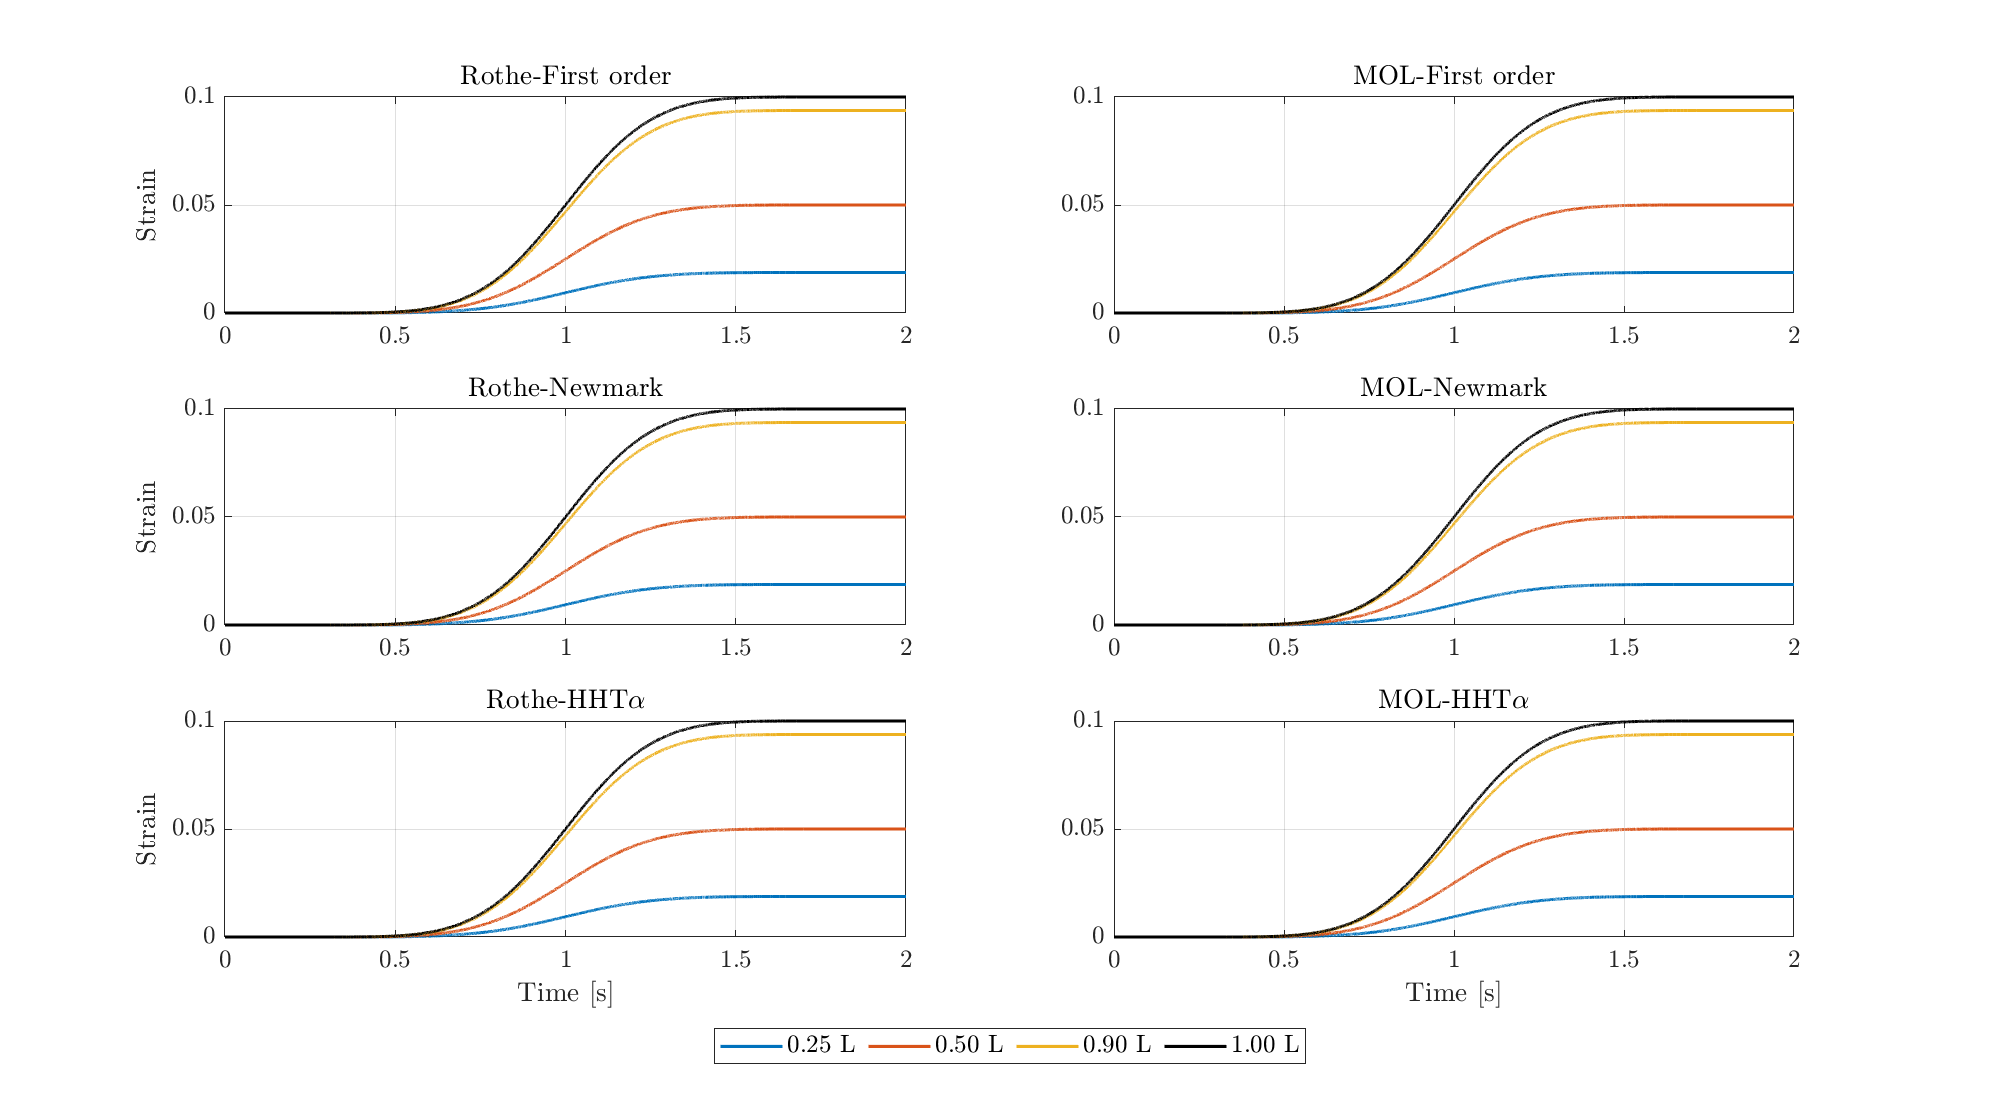
\includegraphics[width=0.99\textwidth]{nh_smooth_disp.eps}
    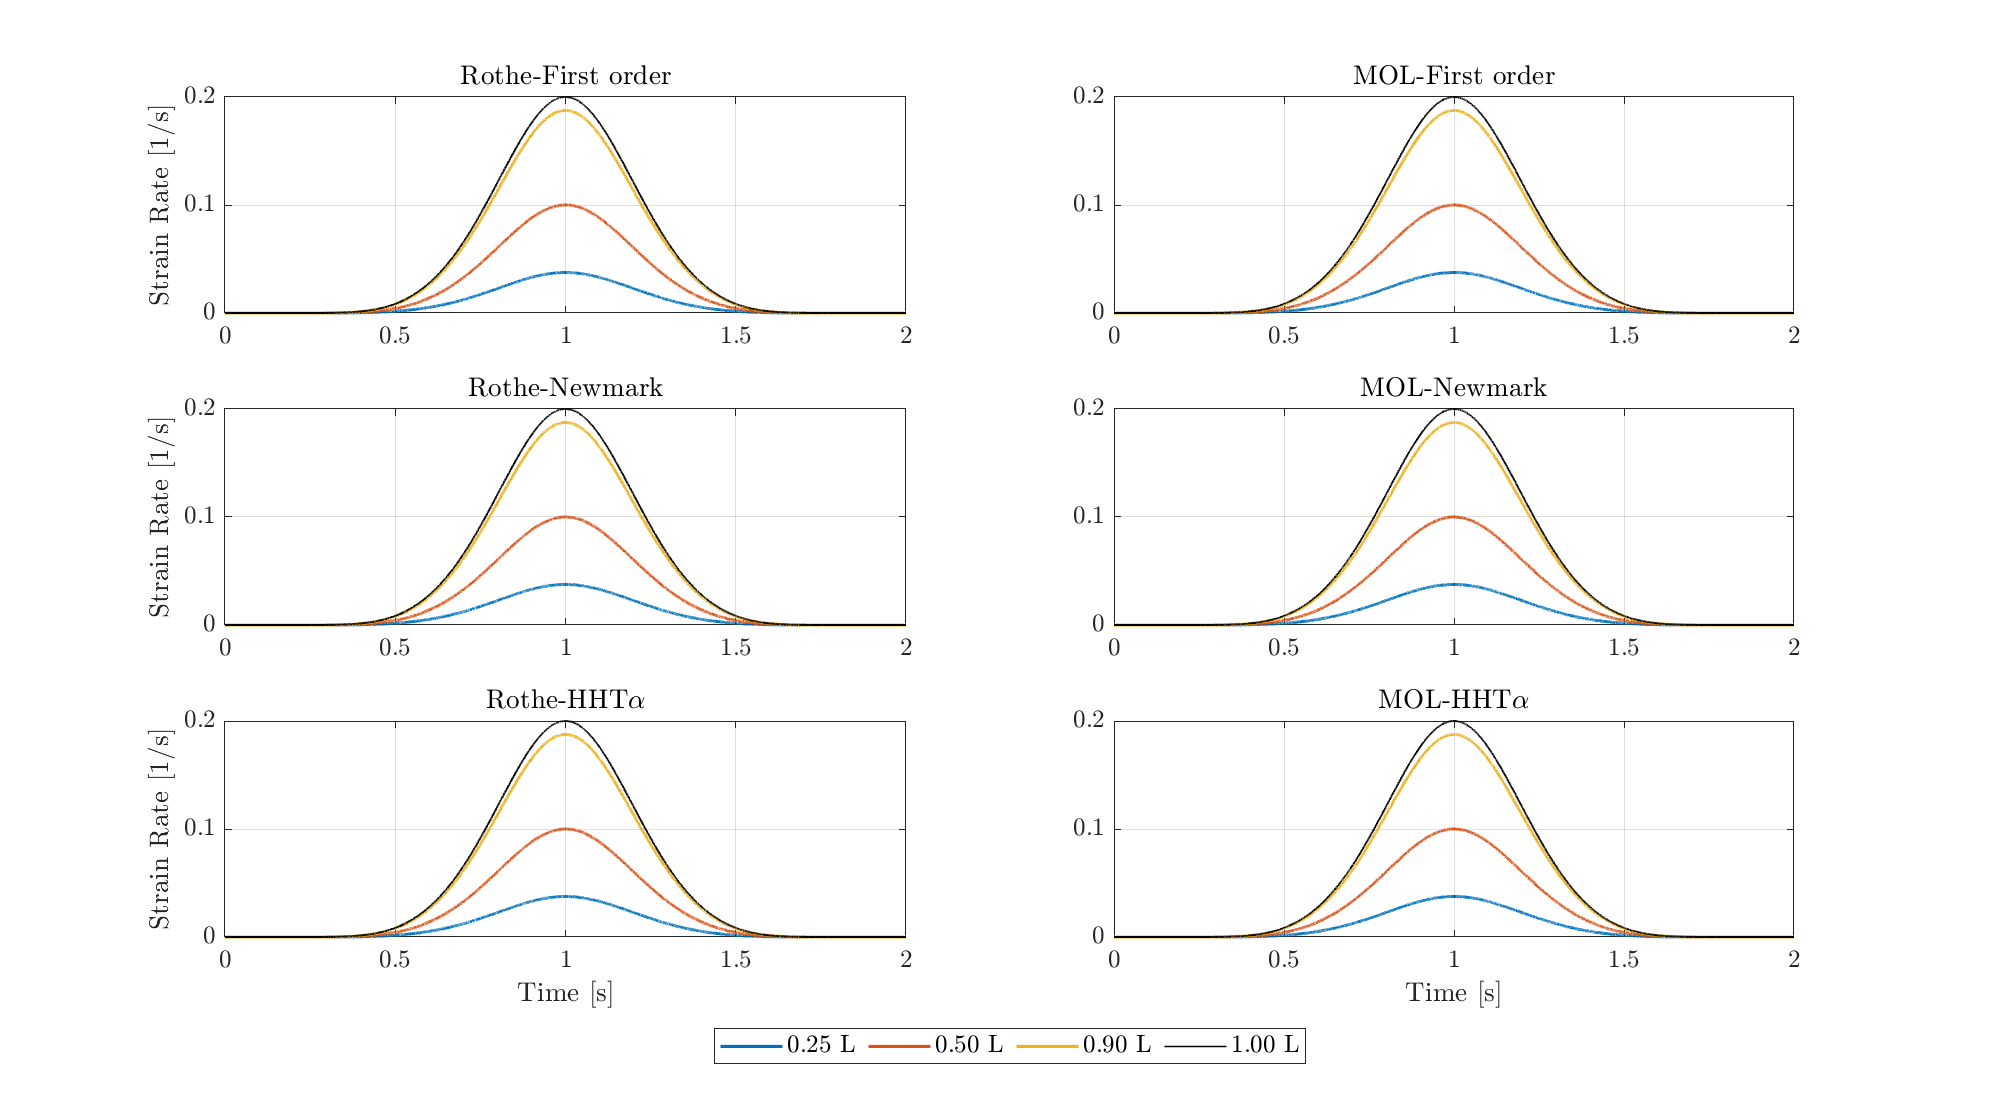
\includegraphics[width=0.99\textwidth]{nh_smooth_vel.eps}
    \caption{Strains (top half) and strain rates (bottom half) for the lengthening experiment using the $C^\infty$ boundary condition \eqref{eq:smooth_pull} at four different locations: $x = 0.25L$, $x=0.5L$, $x=0.9L$, and $x=L$.
    \label{fig:smooth_pull}}
\end{figure}

\begin{figure}
    \centering
    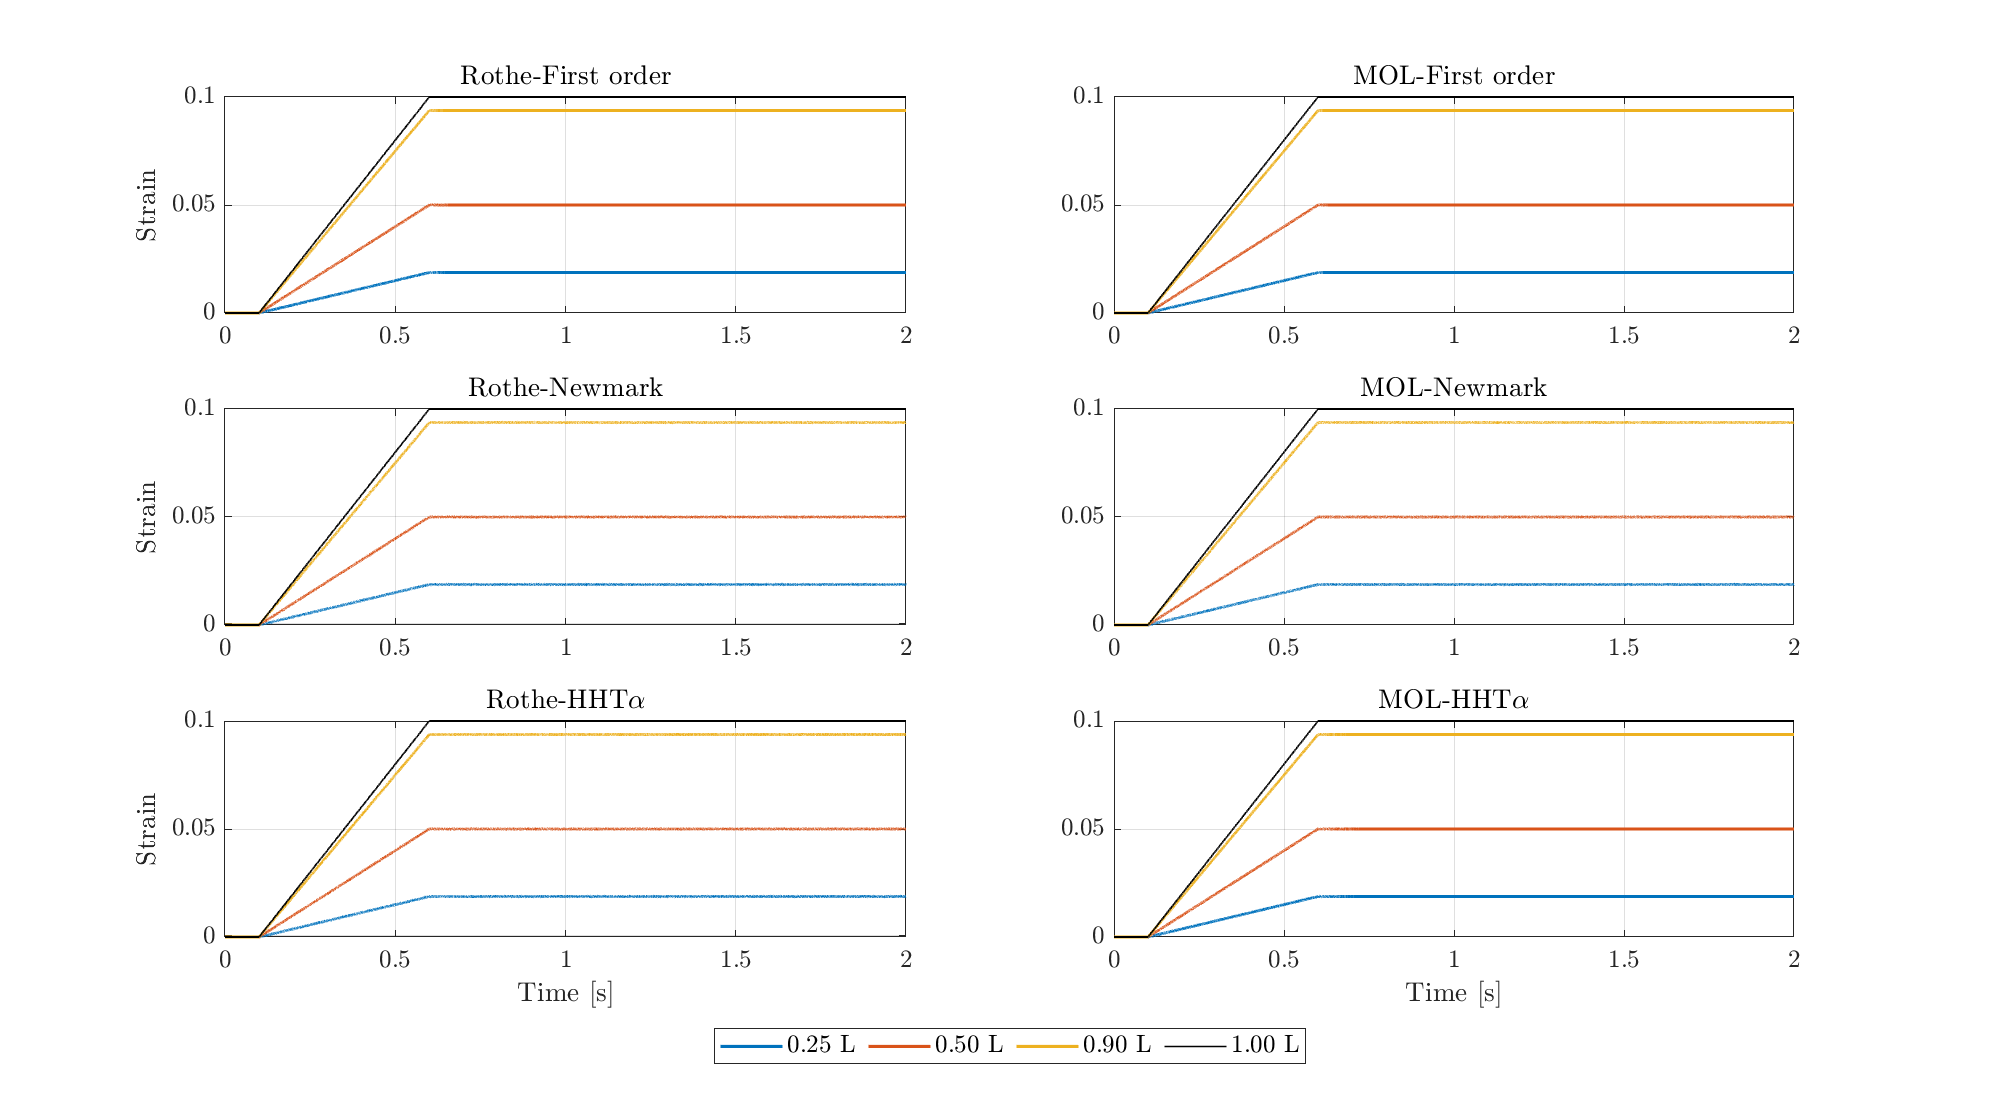
\includegraphics[width=0.99\textwidth]{nh_linear_disp_1.eps}
    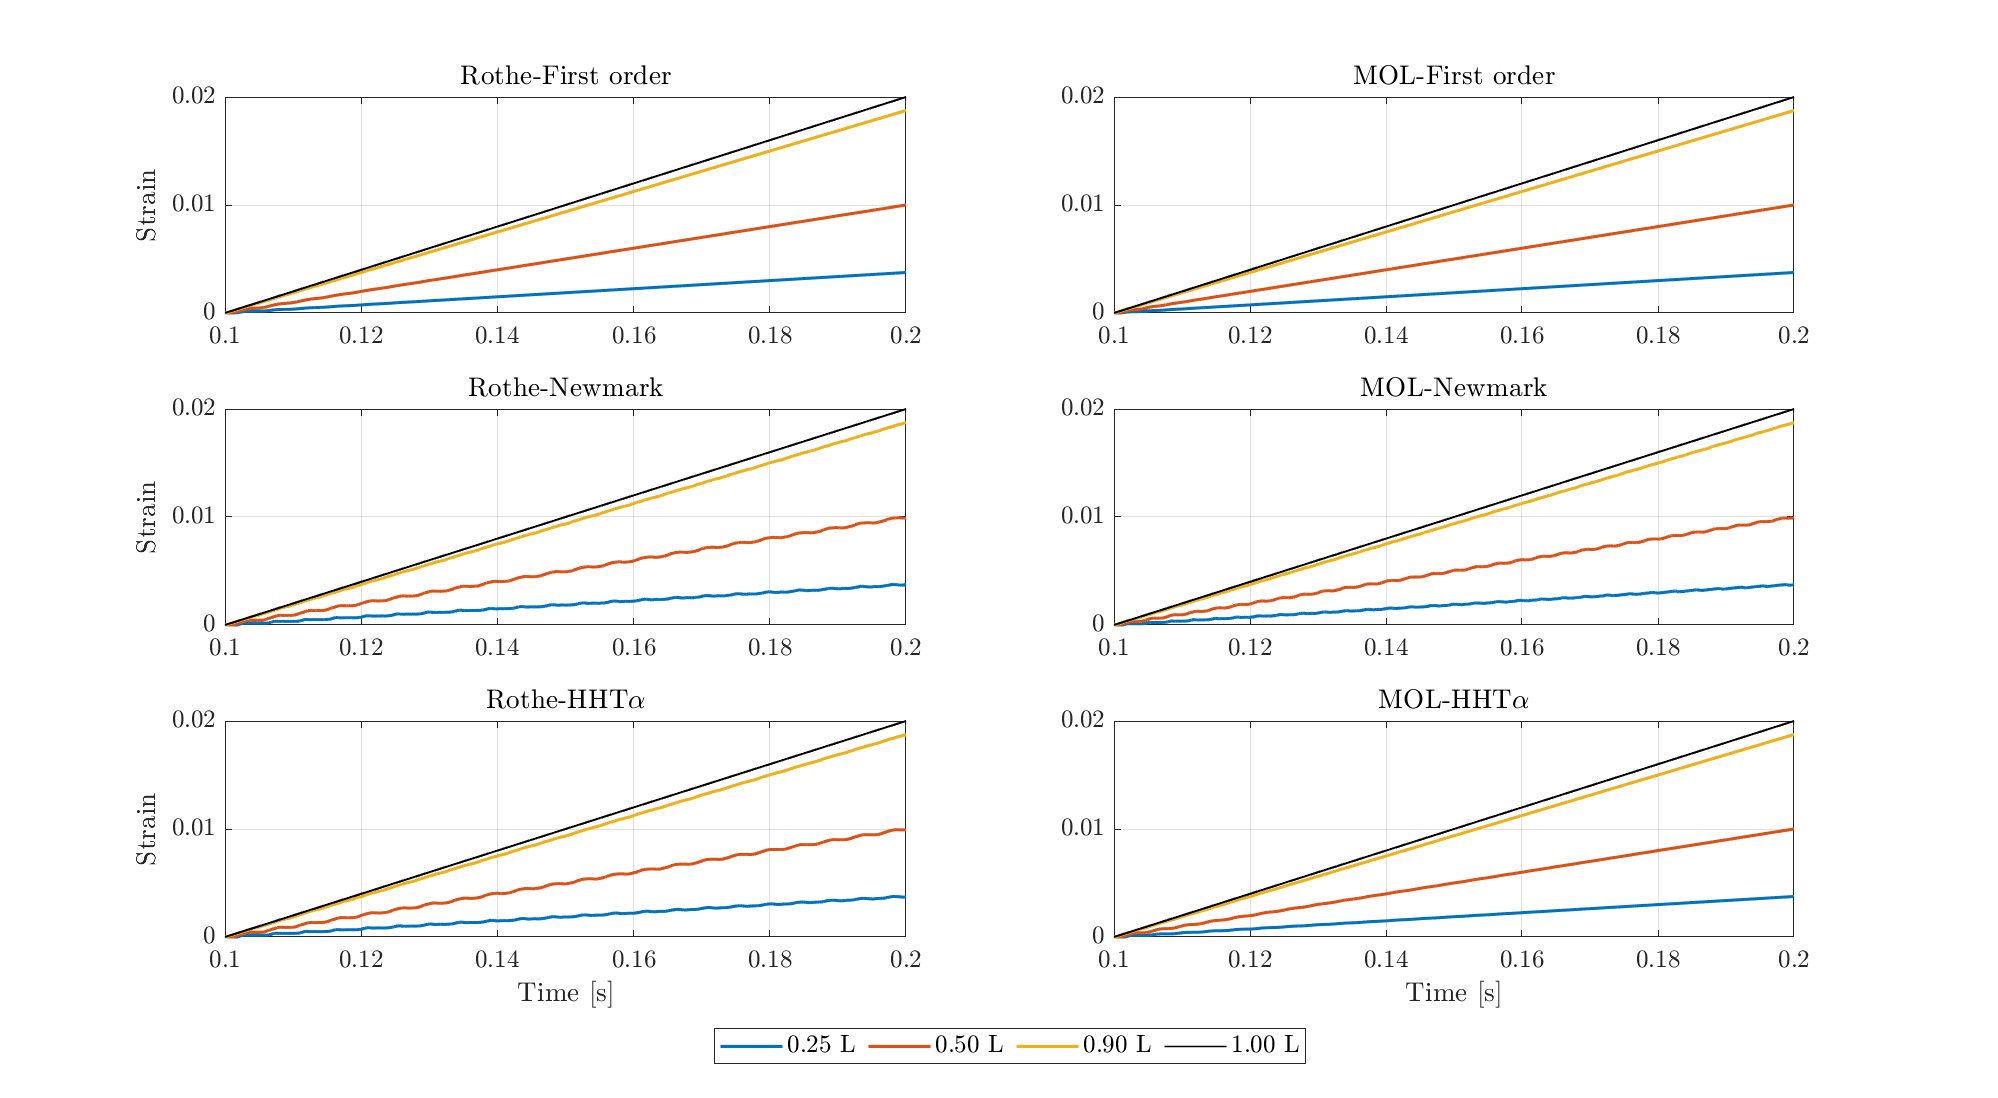
\includegraphics[width=0.99\textwidth]{nh_linear_disp_2.eps}
    \caption{Strains over $t \in [0,2]$ (top half) and a zoomed version to $t \in [0,0.2]$ (bottom half) at four different locations: $x = 0.25L$, $x=0.5L$, $x=0.9L$, and $x=L$. Lengthening experiment performed using the linear profile \eqref{eq:lin_pull}.
    \label{fig:lin_pull_disp}}
\end{figure}

\begin{figure}
    \centering
    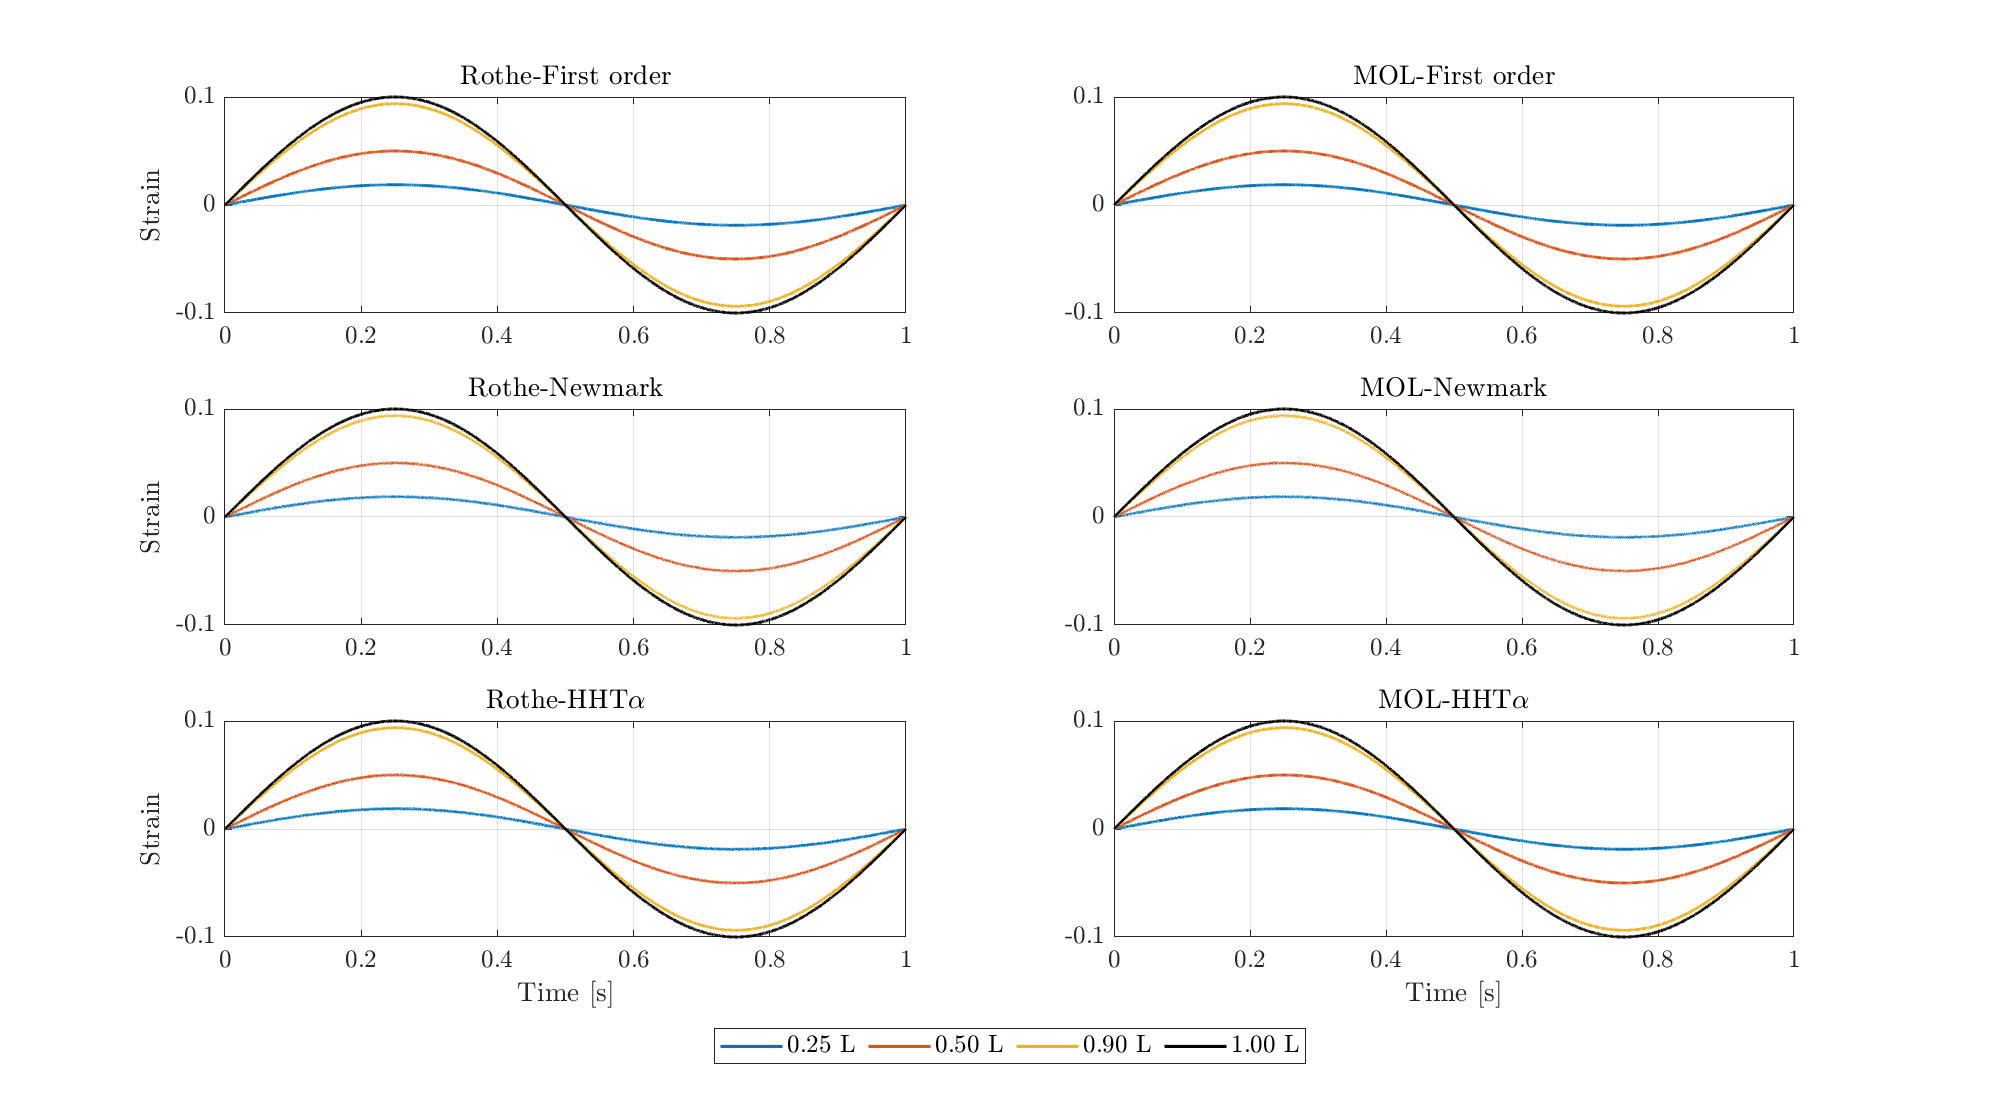
\includegraphics[width=0.99\textwidth]{nh_sin_disp_1.eps}
    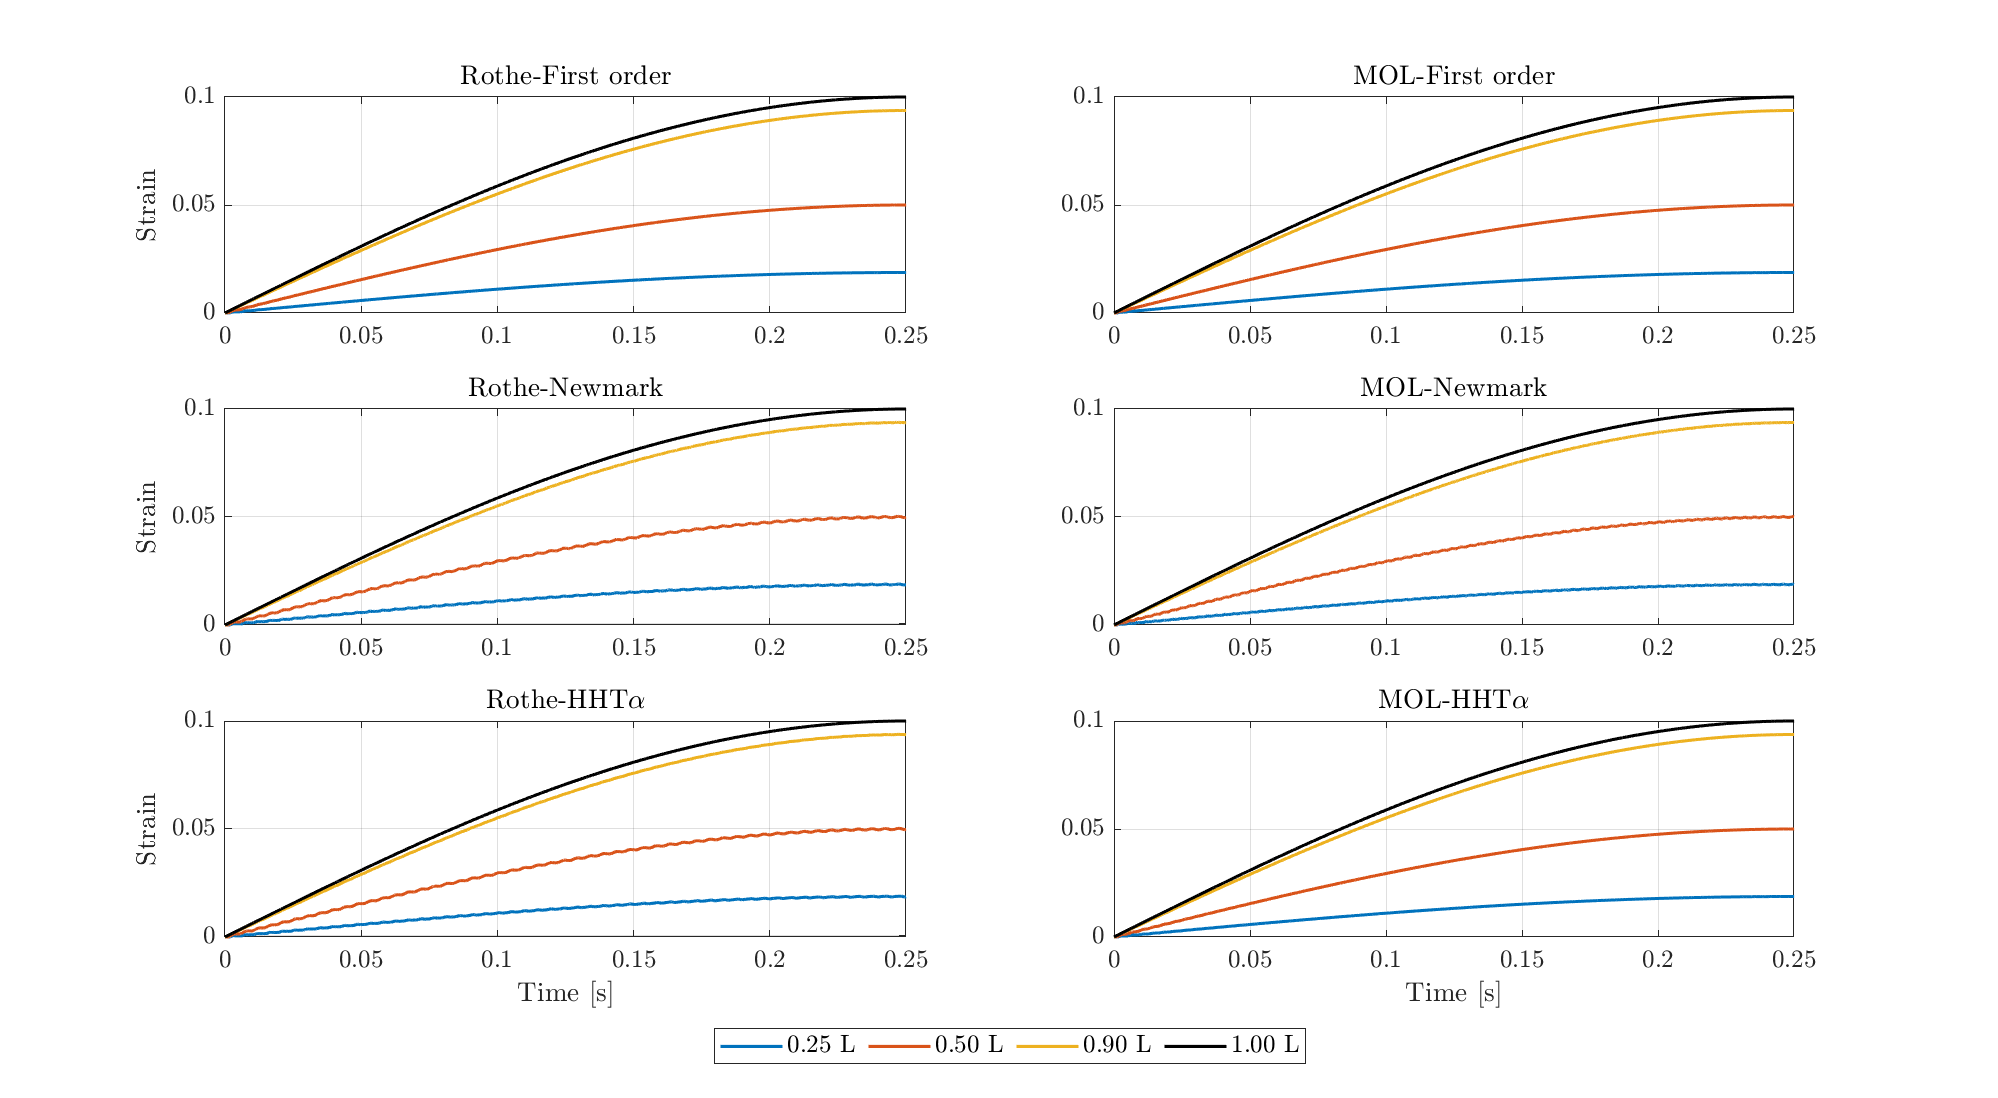
\includegraphics[width=0.99\textwidth]{nh_sin_disp_2.eps}
    \caption{Strains over $t \in [0,1]$ (top half) and a zoomed version to $t \in [0,0.25]$ (bottom half) at four different locations: $x = 0.25L$, $x=0.5L$, $x=0.9L$, and $x=L$. Lengthening experiment performed using the sinusoidal profile \eqref{eq:sin_pull}.
    \label{fig:sin_pull_disp}}
\end{figure}

\begin{figure}
    \centering
    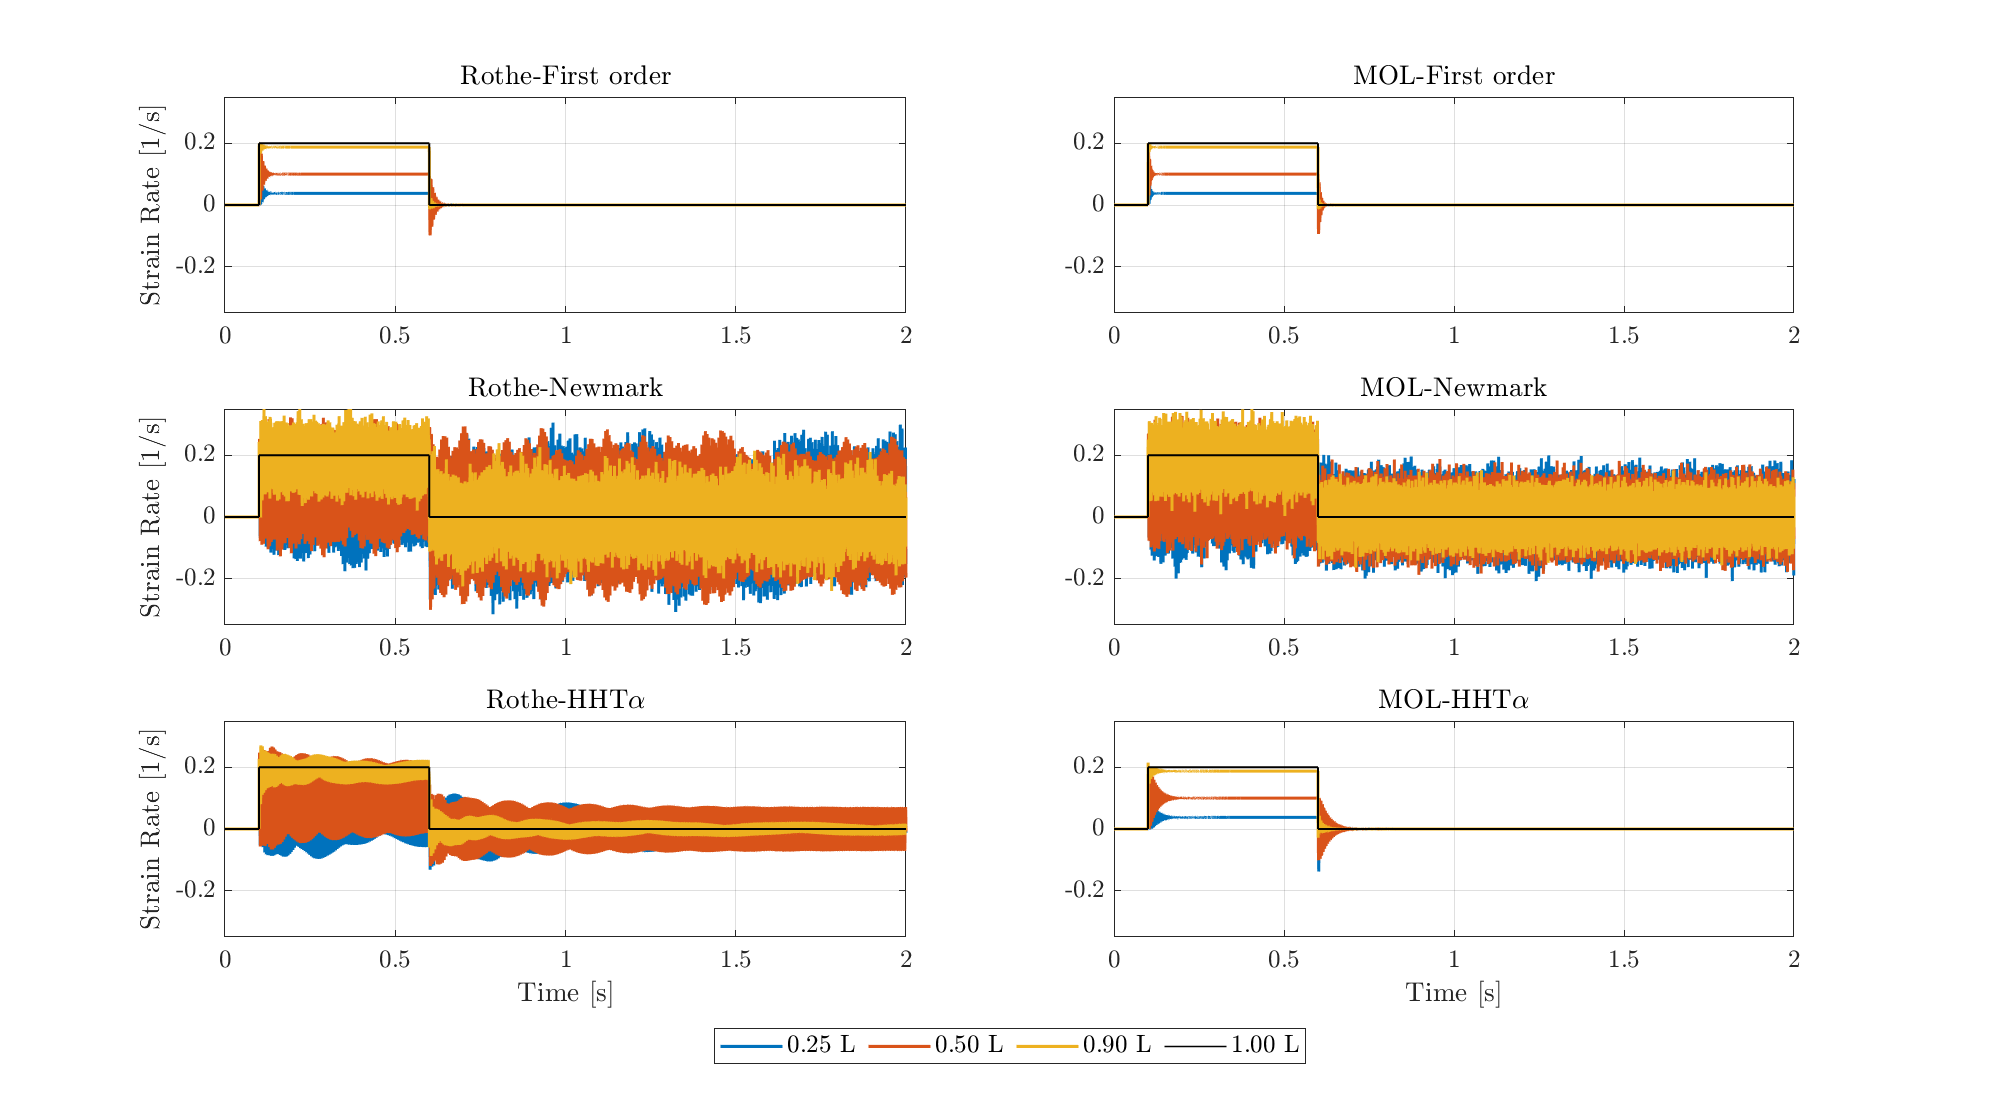
\includegraphics[width=0.99\textwidth]{nh_linear_vel_1.eps}
    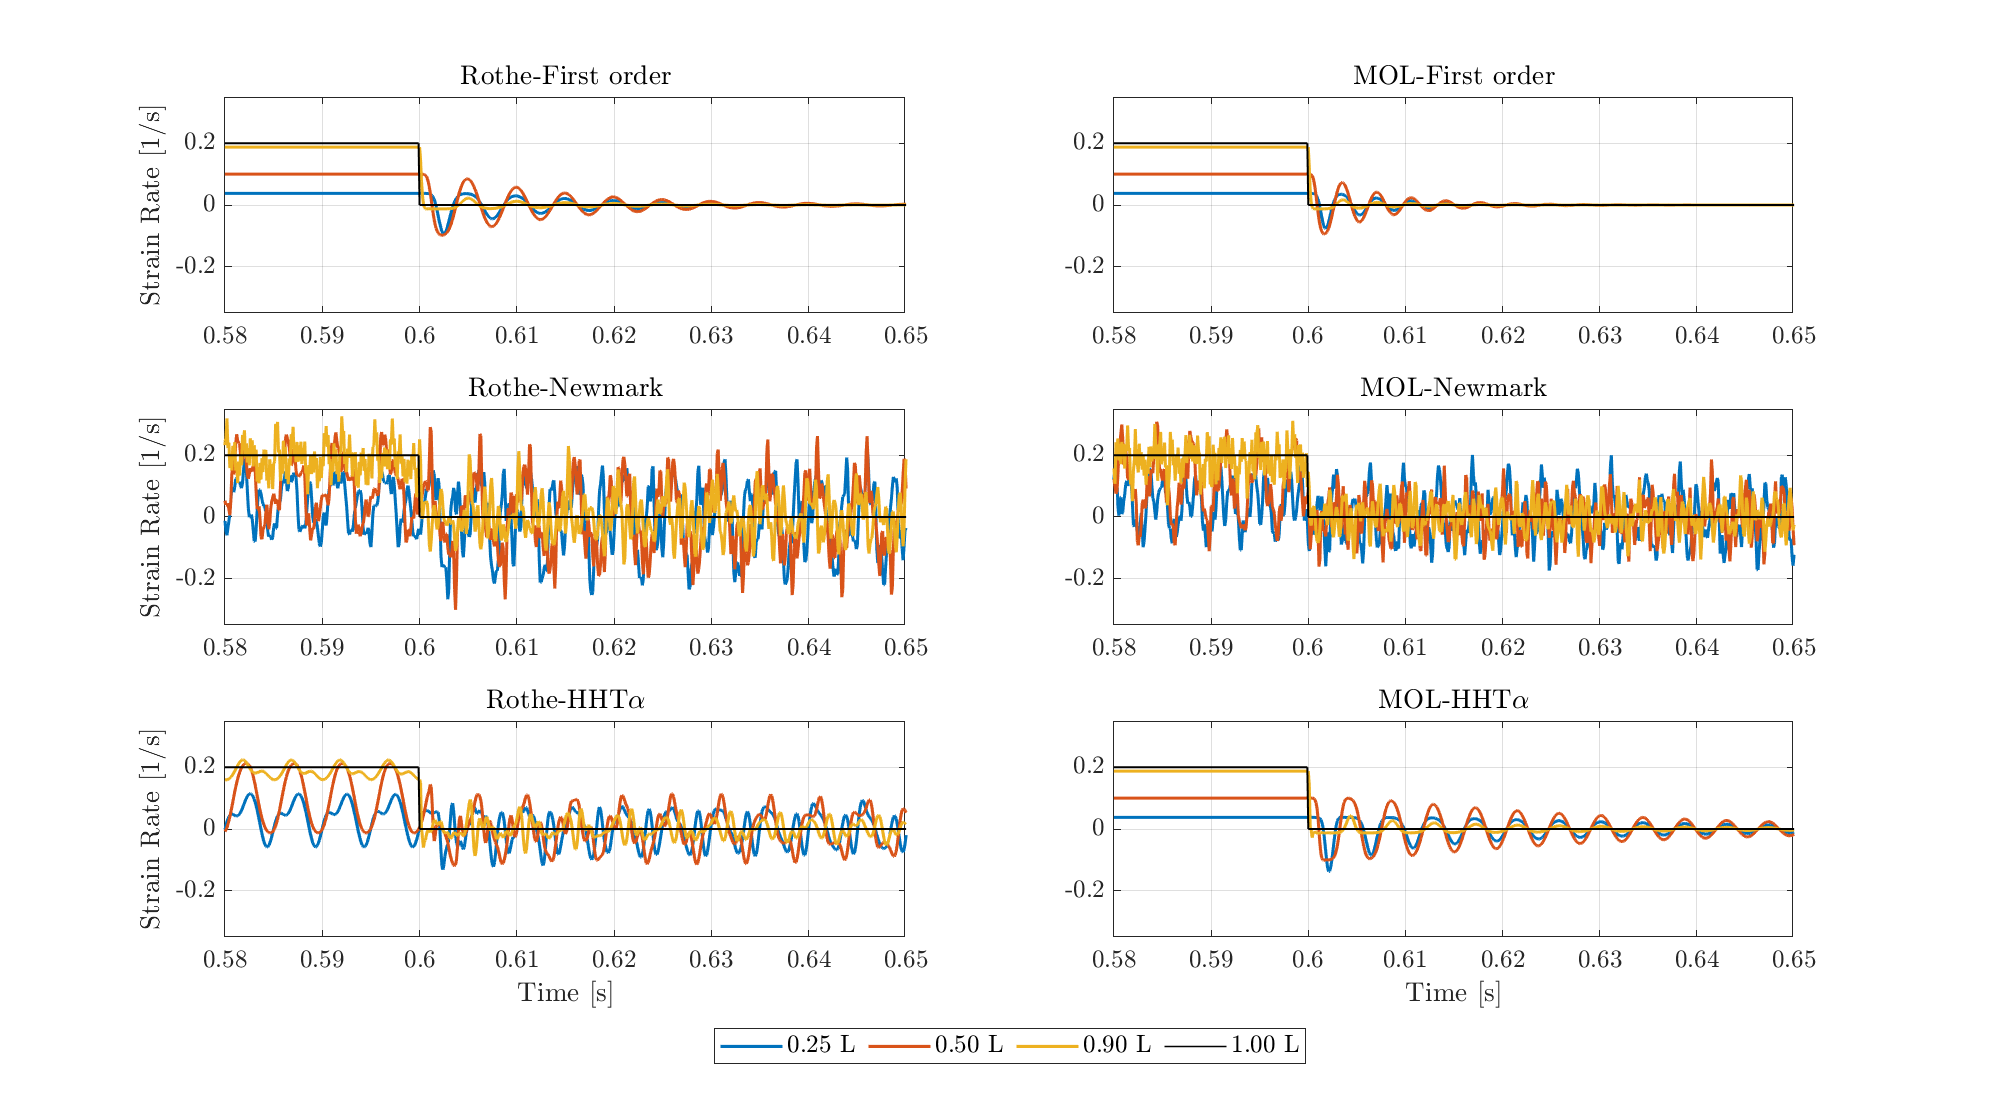
\includegraphics[width=0.99\textwidth]{nh_linear_vel_2.eps}
    \caption{Strain rates over $t \in [0,2]$ (top half) and a zoomed version to $t \in [0.58,0.65]$ where the (prescribed) strain rate jumps from 0.2 \si{s^{-1}} to 0 \si{s^{-1}} (bottom half)  at four different locations: $x = 0.25L$, $x=0.5L$, $x=0.9L$, and $x=L$. Lengthening experiment performed using the linear profile \eqref{eq:lin_pull}.
    \label{fig:lin_pull_vel}}
\end{figure}

\begin{figure}
    \centering
    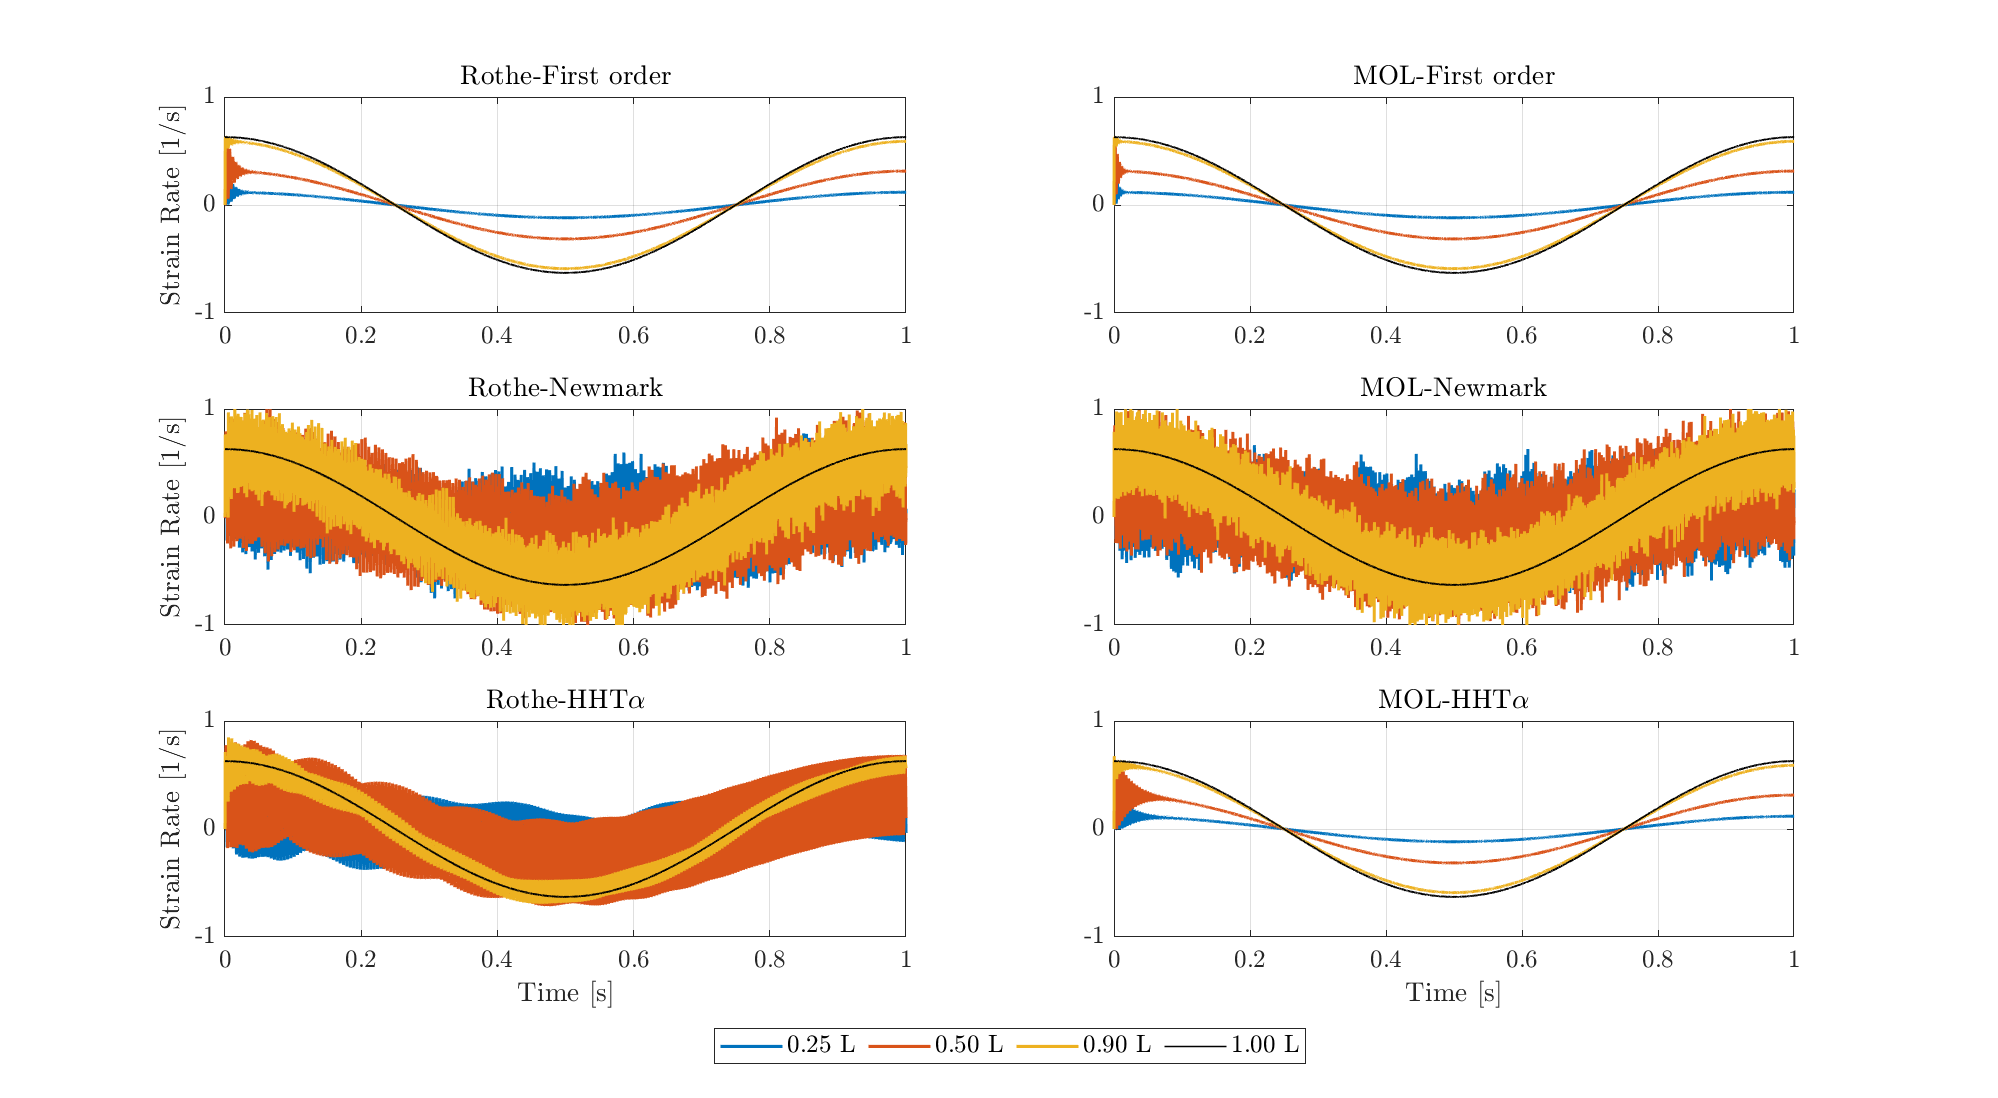
\includegraphics[width=0.99\textwidth]{nh_sin_vel_1.eps}
    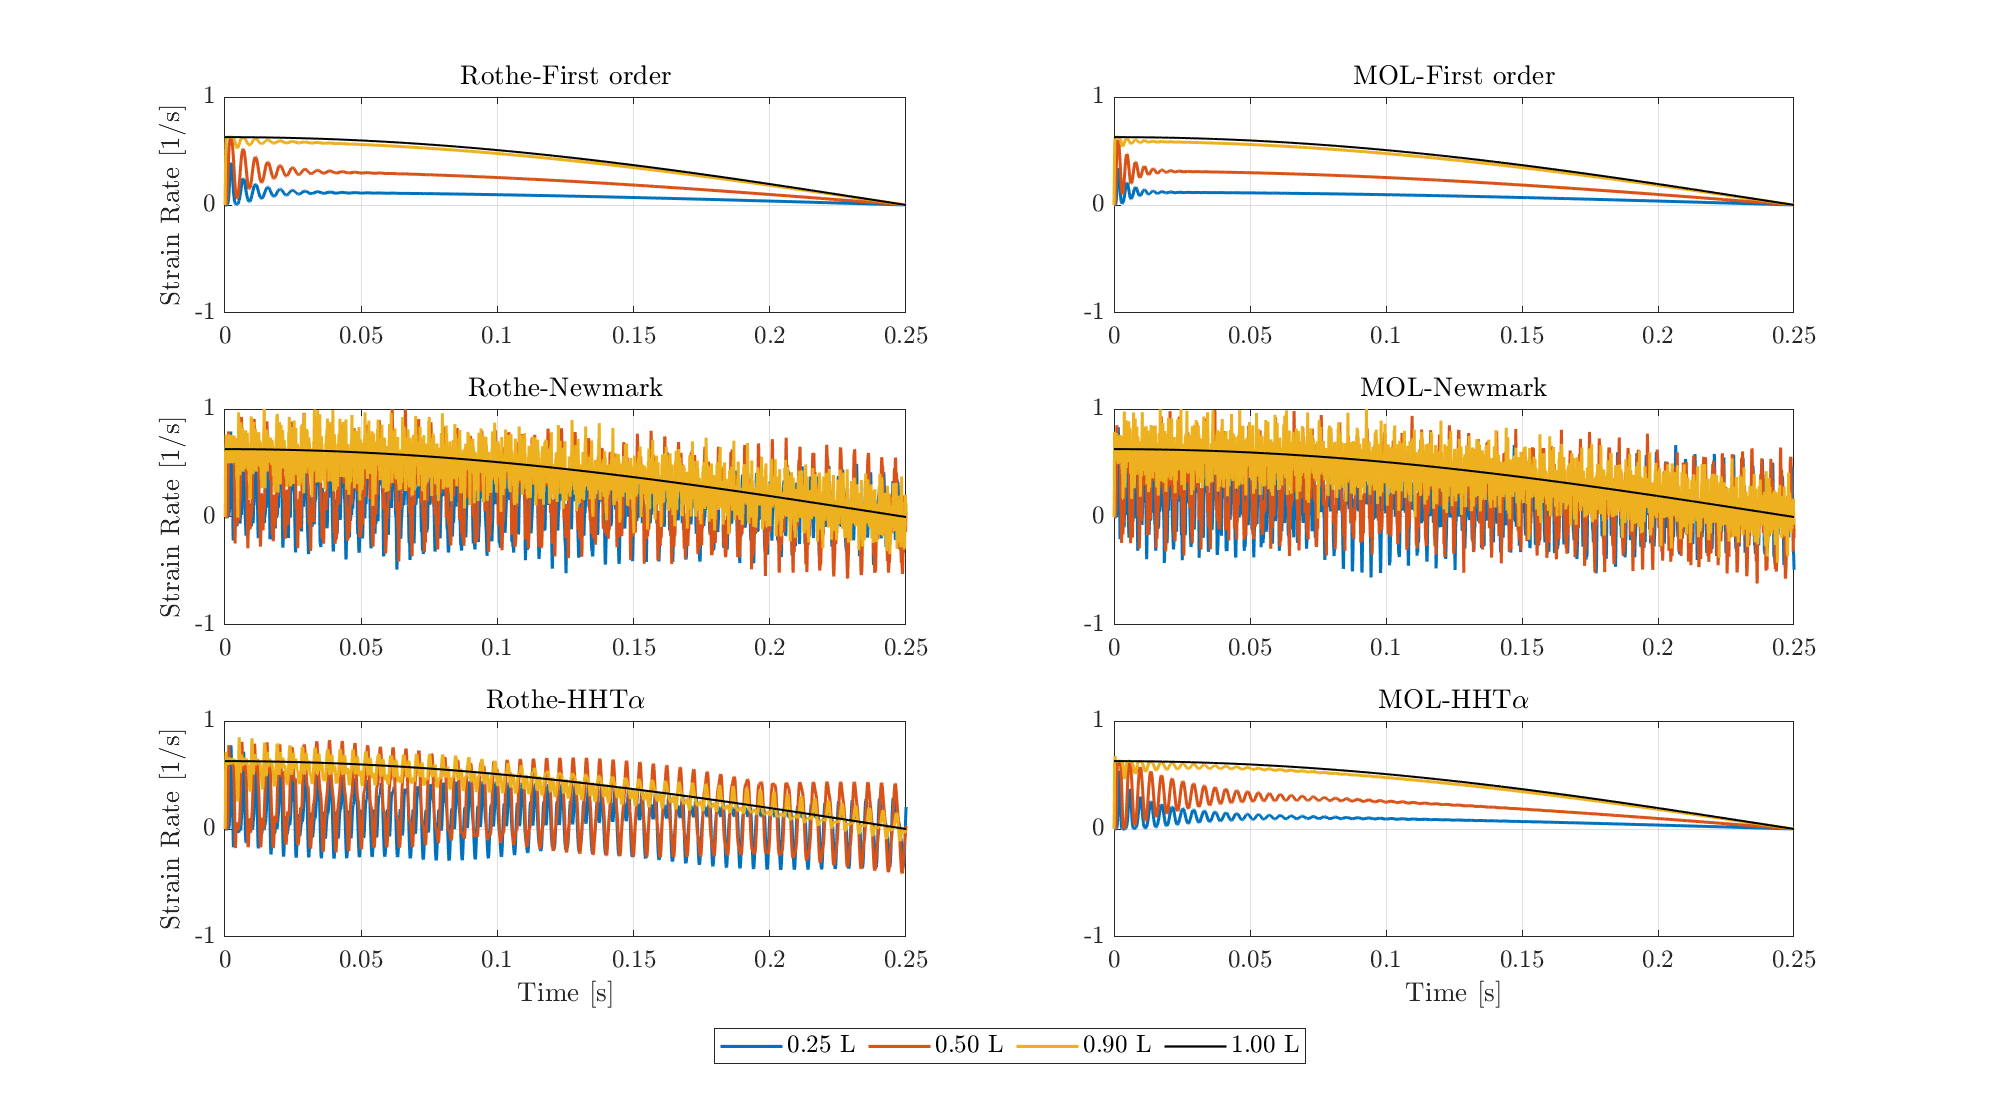
\includegraphics[width=0.99\textwidth]{nh_sin_vel_2.eps}
    \caption{Strain rates over $t \in [0,1]$ (top half) and a zoomed version to $t \in [0,0.25]$ showcasing the nonzero velocity at the beginning (bottom half) at four different locations: $x = 0.25L$, $x=0.5L$, $x=0.9L$, and $x=L$. Lengthening experiment performed using the sinusoidal profile \eqref{eq:lin_pull}.
    \label{fig:sin_pull_vel}}
\end{figure}


\subsection*{An IMEX scheme}

We can also test an implicit-explicit (IMEX) scheme for the nonlinear system of equations \eqref{eq:mol}. Observe from the definition of $\*K(\*U)$ in \eqref{eq:mol_first_order_def_stiffness_vector} that:
\begin{multline}
    \quad \*K(\*U)_T = \mathcal{L}_\mu \underbrace{\left( B^{-1} \int_{\widehat{T}} [\widehat{\*D} \widehat{\*P}]^\top [\widehat{\*D} \widehat{\*P}] \right)}_{=: \widetilde{\*K}_T} [\*u(t)] \\
    + \underbrace{\int_{\widehat{T}} \dfrac{\mathcal{L}_\lambda \log \left( B^{-1}[\widehat{\*D} \widehat{\*P}] [\*u(t)] + 1 \right) - \mathcal{L}_\mu}{\mathcal{L}_\lambda} [\widehat{\*D} \widehat{\*P}]^\top}_{=: \widetilde{\*F_1}(\*U)_T} + \mathcal{L}_\mu \underbrace{\int_{\widehat{T}} [\widehat{\*D} \widehat{\*P}]^\top}_{=: \widetilde{\*F_2}_T}. \quad
\end{multline}
Thus, we can write:
\begin{equation}
    \*K(\*U) = \mathcal{L}_\mu \widetilde{\*K} \*U + \widetilde{\*F_1}(\*U) + \mathcal{L}_\mu \widetilde{\*F_2},
\end{equation}
where 
\begin{equation}
    \widetilde{\*K} = \assembly_{T \in \mathcal{T}_h} \widetilde{\*K}_T, \quad \widetilde{\*F_1}(\*U) = \assembly_{T \in \mathcal{T}_h} \widetilde{\*F_1}(\*U)_T, \quad \widetilde{\*F_2} = \assembly_{T \in \mathcal{T}_h} \widetilde{\*F_2}_T.
\end{equation}
Therefore, the MOL system \eqref{eq:mol} can be written as:
\[
	\*M \ddot{\*U} + \mathcal{L}_\mu \widetilde{\*K} \*U + \widetilde{\*F_1}(\*U) + \mathcal{L}_\mu\widetilde{\*F_2} = \*0.
\]
Defining once again $\*V:=\dot{\*U}$ we can propose the following scheme:
\begin{subequations} \label{eq:TS-mol-imex}
    \begin{align}
        &\dfrac{\*U^{n+1} - \*U^n}{\Delta t} = \*V^{n+1} \\
	    \label{eq:TS-mol-imex-b} &\*M \left( \dfrac{\*V^{n+1} - \*V^n}{\Delta t} \right) + \mathcal{L}_\mu \widetilde{\*K} \*U^{n+1} = -\widetilde{\*F_1}(\*U^n) - \mathcal{L}_\mu \widetilde{\*F_2}.
    \end{align}
\end{subequations}
This means that we treat the linear term \textit{implicitly} and the nonlinear term \textit{explicitly}. In this way, writing Equation \eqref{eq:TS-mol-imex-b} in terms of displacements, we obtain:
\begin{equation}
	\left( \*M + \mu \Delta t^2 \widetilde{\*K} \right)\*U^{n+1} = \*M(\*U^n + \Delta t \*V^n) - \Delta t^2 \*F_1(\*U^n) - \mu \Delta t^2 \*F_2.
\end{equation}
No nonlinear solver is needed. However, numerical experiments for the linear boundary condition \eqref{eq:lin_pull} show that this method does not compute better velocities than any of the previously presented methods (see Figure \ref{fig:lin_pull_imex}). Furthermore, this method behave more like an explicit method, since the largest time step size that was allowed was $\Delta t = 5 \cdot 10^{-6}$ s (compare this to the rest of the experiments in which $\Delta t  = 10^{-4}$ s, of course with larger time step sizes being possible). This also shows that the stiffness in this problem comes from the nonlinear part of \eqref{eq:neohookean_stress_1d}, rather than from the linear part.

\begin{figure}
    \centering
    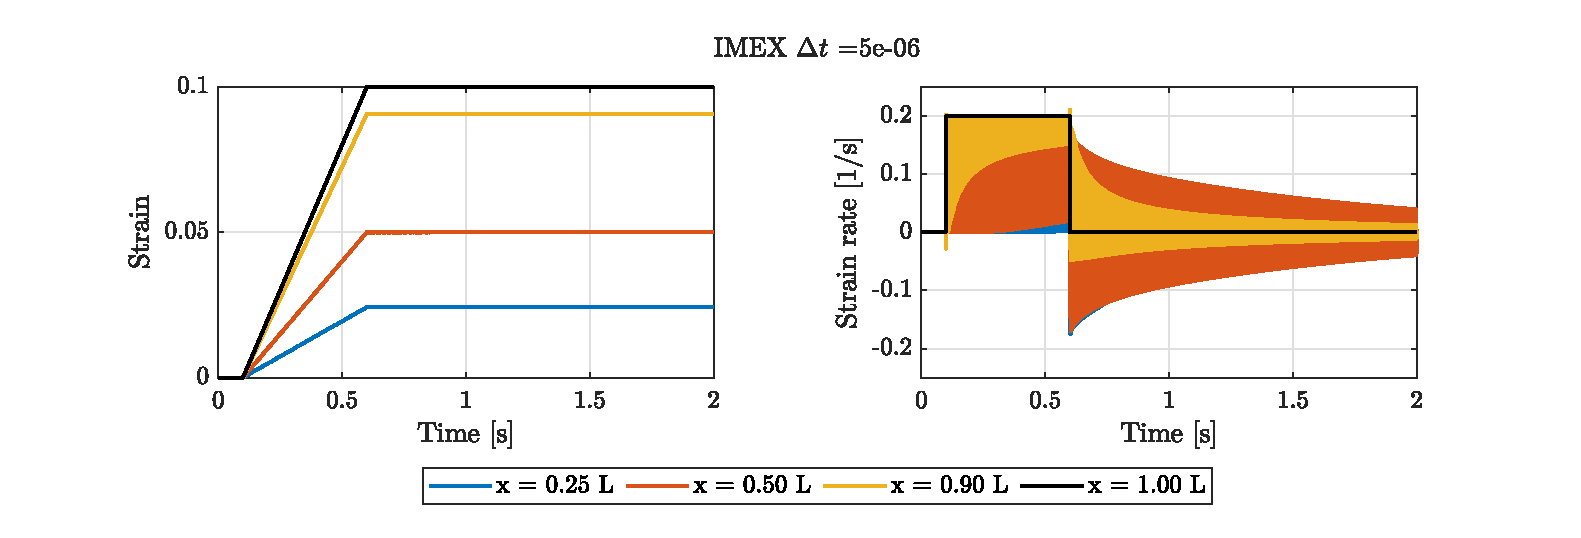
\includegraphics[width=0.99\textwidth]{nh_imex.eps}
    \caption{Strain (left) and strain rate (right) profiles at four different locations ($x = 0.25L$, $x=0.5L$, $x=0.9L$, and $x=L$) for the lengthening experiment using the linear profile \eqref{eq:lin_pull} and an IMEX time stepping scheme ($\Delta x = L/64$, $\Delta t = 0.5 \cdot 10^{-6}$).
    \label{fig:lin_pull_imex}}
\end{figure}

\subsection*{Matlab's built-in solvers}

Once the MOL system \eqref{eq:mol} is constructed, many time-stepping schemes for ODE
systems can be tested, including built-in Matlab solvers. For this set of
experiments, we consider the sinusoidal pull \eqref{eq:sin_pull} and no time step restrictions, thus letting Matlab choose the best time step for the given tolerances
(\texttt{RelTol} = $10^{-2}$, \texttt{AbsTol} = $10^{-4}$). The MOL equations are solved as a square system of 2 $\times$ (DOF-2) equations (DOF$=2N-1$). 

We show in Table \ref{tab:mol_matlab_solvers} a summary of the performance of 
each Matlab solver. As expected, most of the non-stiff
solvers did not work (they would achieve $\lambda = \partial_x u + 1 \leq 0$ at
some iteration), with the exception being \texttt{ode113}. This is a variable-step, variable-order (VSVO) Adams-Bashforth-Moulton PECE (Predict-Evaluate-Correct-Evaluate) solver that uses orders up to 12 but applies a 13th-order formula for error estimation and local extrapolation. As a multistep solver, it relies on solutions from several previous time points to compute the current step. It can be more efficient than \texttt{ode45} for stringent tolerances or when evaluating the ODE function is particularly costly \cite{ShampineReichelt1997}.

The solver \texttt{ode23tb} gave the best results. Not only it took
the shortest time to compute a solution but also allowed for the largest time step of all Matlab solvers. However, the relatively crude tolerance chosen to run these experiments might have played a fundamental role. According to \cite{ShampineReichelt1997}, \texttt{ode23tb} is an implicit Runge-Kutta solver based on the TR-BDF2 formula, combining a trapezoidal rule step with a second-stage backward differentiation formula. It reuses the same iteration matrix for both stages, improving efficiency. Like \texttt{ode23s} and \texttt{ode23t}, it can be more efficient than \texttt{ode15s} for problems with crude tolerances.

We show, in particular, the velocities and the time step sizes for the solvers that finished their computation (according to Table \ref{tab:mol_matlab_solvers}) in Figure \ref{fig:sin_pull_matlab}. We observe that only \texttt{ode23s} and \texttt{ode23tb} computed velocities somewhat similar to those in Figure \ref{fig:sin_pull_vel}, but overshooting was still a problem in these solvers. Moreover, the time step size chosen by these solvers was in line with the one considered for Figure \ref{fig:sin_pull_vel}.

\begin{table}
	\centering
	\begin{tabular}{|c|c|c|c|}\hline
		Solver & Finished? & Avg. $\Delta t$ [s] & CPU Time [s] \\\hline
		ode45 & No & - & -  \\\hline
		ode23 & No & - & -  \\\hline
		ode113 & Yes & $1.46 \cdot 10^{-6}$ & 724  \\\hline
		ode78 & No & - & -   \\\hline
		ode89 & No & - & -   \\\hline
		ode15s & No & - & -  \\\hline
		ode23s & Yes & $5.69 \cdot 10^{-5}$ & 2,262 \\\hline
		ode23t & Yes & $6.21 \cdot 10^{-7}$ & 1,301 \\\hline
		ode23tb & Yes & $4.25 \cdot 10^{-5}$ & 29  \\\hline
	\end{tabular}
	\caption{Performance of Matlab's adaptive solvers for the MOL system \eqref{eq:mol} and the lengthening experiment using the sinusoidal profile \eqref{eq:sin_pull} as boundary condition ($\Delta x = L/64$). For \texttt{ode23s}, the Jacobian was (numerically) computed at each time step by the solver. \label{tab:mol_matlab_solvers}}
\end{table}

\begin{figure}
    \centering
    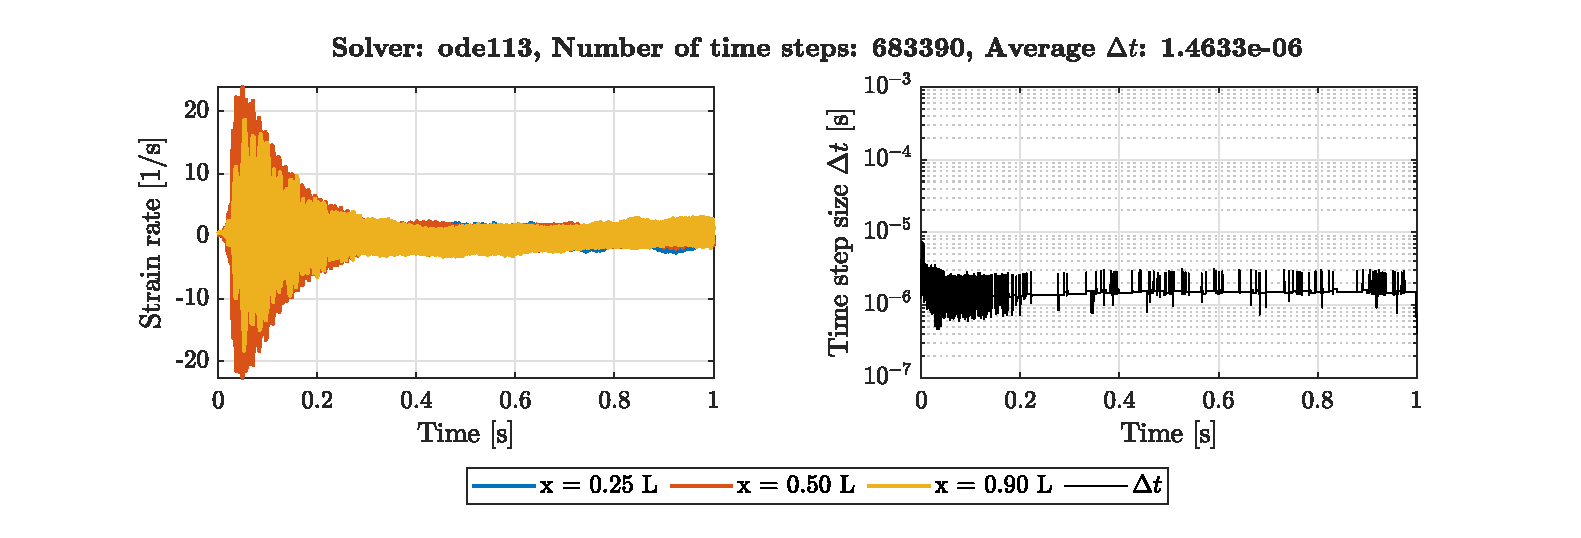
\includegraphics[width=0.99\textwidth]{nh_ode113.eps}
    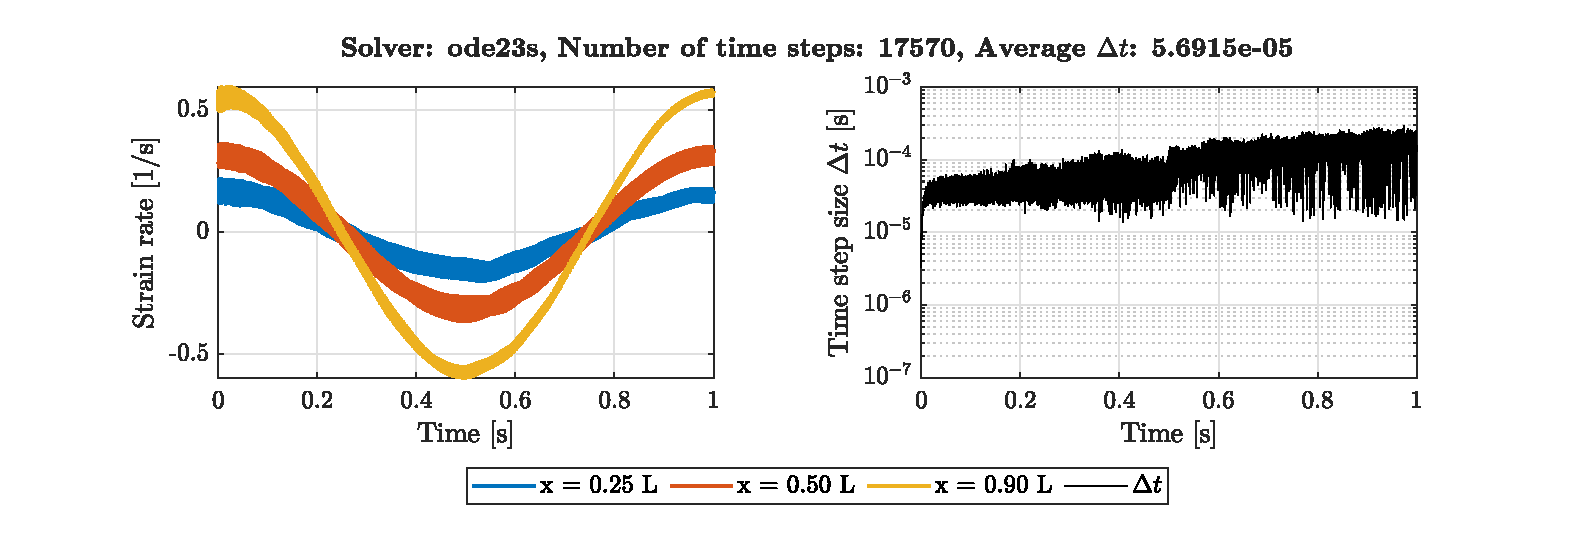
\includegraphics[width=0.99\textwidth]{nh_ode23s.eps}
    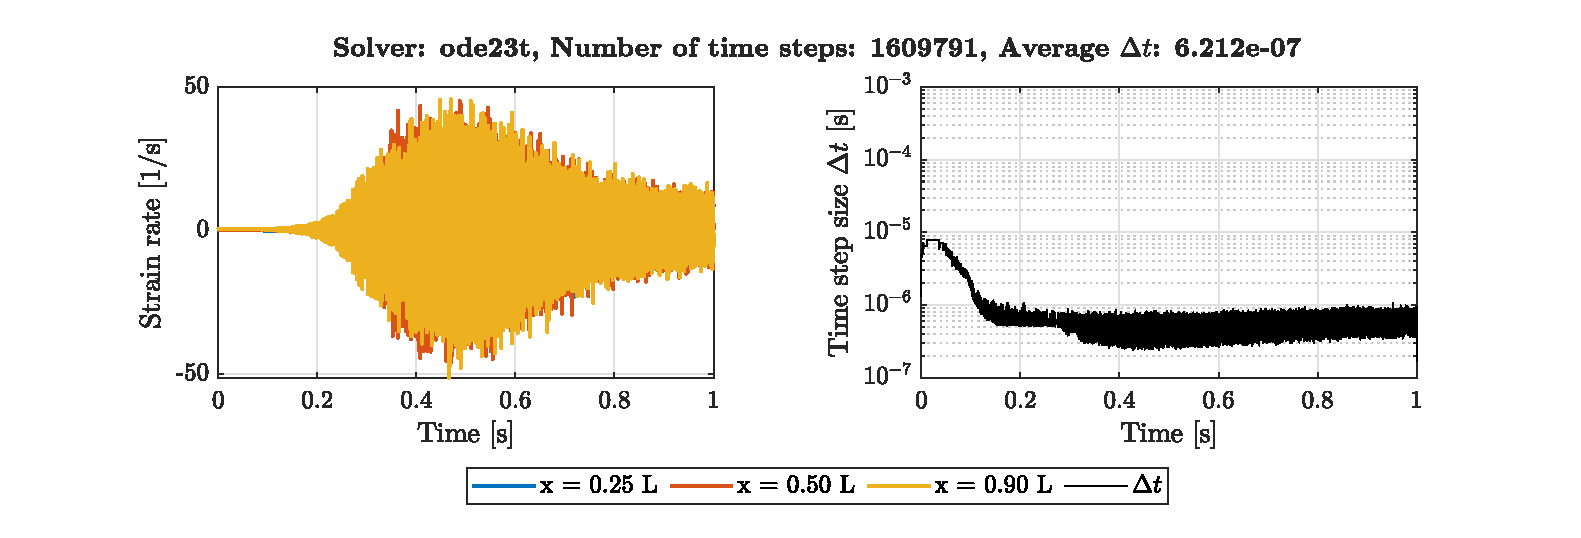
\includegraphics[width=0.99\textwidth]{nh_ode23t.eps}
    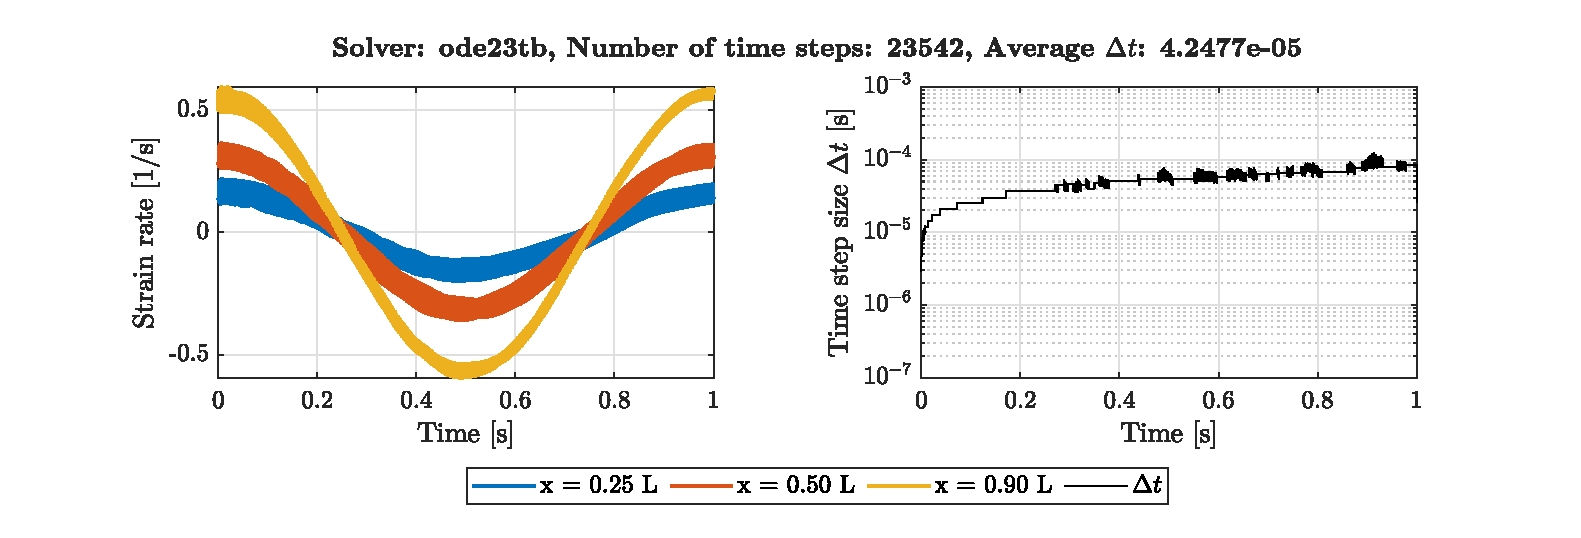
\includegraphics[width=0.99\textwidth]{nh_ode23tb.eps}
    \caption{Strain rates (left column) and time step sizes (right column) for the Matlab solvers that finished solving the lengthening experiment (see Table \ref{tab:mol_matlab_solvers}).
    \label{fig:sin_pull_matlab}}
\end{figure}

\section{Discussion}

If studying Neo-Hookean dynamics was our ultimate goal, the conclusion would be that any of the six methods mentioned at the beginning of the previous section can be used as a time stepping scheme in a 1D or 3D elastic model. This primarily because the stress $P$ only depends on the stretch $\lambda$, and therefore, only on the displacement field. However, since our main goal is to find a time stepping scheme suitable for skeletal muscle dynamics, our methods need to compute ``good'' displacements \textbf{and} velocities since, in this case, the stress will depend on both stretch and strain rates as a \textbf{multiplicative} term. By ``good'' we consider, for now, displacements and velocities free of unrealistic, high-frequency oscillations, and if they are present, they must get dissipated quickly. Thus, only three methods can become candidates for a 3D code: Rothe-First order, MOL-First order, and MOL-HHT-$\alpha$. 

Furthermore, from the experiments performed with the IMEX scheme \eqref{eq:TS-mol-imex}, as well as with Matlab's built in solvers, we expect that problems of this flavour will require rather small time step sizes. This does not contradict the unconditional stability of the fully implicit schemes presented here. While larger time step sizes are allowed for a linear problem, taking one that is too large in a nonlinear problem can lead to a loss of convergence in the nonlinear solver. 

At this juncture, choosing which method to use becomes a software engineering decision. On the one hand, choosing the Rothe-First order method would allow us to reuse some of the computational developments by Dominguez \cite{Seba} and implement them in a fully dynamic code. Thus, that code would only need to be \textit{refactored} for our purposes. Moreover, this choice would allow for adaptive refinement to be added in the future. On the other hand, moving forward with a MOL approach would require us to almost completely \textit{rewrite} the code developed in \cite{Seba}. Therefore, we decide to discretize the 3D dynamic model using Rothe-First order method \eqref{eq:rothe_first_order}. 
The choice of a first-order over a second-order method is also justified by the fact that an alternative way to reduce the spurious oscillations in methods such as Newmark's is precisely to take $\gamma > 1/2$, at the expense of losing second-order convergence \cite[Section 8.6]{raviartthomas}.

\section{Conclusion}

We studied the performance of several time stepping schemes for one-dimensional nonlinear elasticity, and in particular, for Neo-Hookean deformation. The first set of methods (first order method, Newmark's method, and the HHT-$\alpha$ method, both in Rothe's and MOL frameworks) gave mixed results for nonsmooth boundary conditions. Only the Rothe-First order, MOL-First order, and MOL-HHT-$\alpha$ methods dealt successfully with overshooting. Next, we tested an IMEX scheme which performed poorly compared to the previous methods. In fact, this method only ran with a very small time step size. Finally, we tested some of Matlab's built-in solvers to assess the time step size they require to return a solution with rather large tolerances. We found that almost all the solvers designed for non-stiff problems, as well as some stiff ones, did not finish their computation. Indeed, only the \texttt{ode113} and \texttt{ode23tb} computed results comparable to those from the MOL-Newmark method (i.e. without dissipation of high-frequency oscillations).
These suggest a first-order implicit method is a good time stepping scheme candidate for the dynamic version of the full 3D model of skeletal muscle deformation.

\part{Three-dimensional elastodynamics}

\chapter{A Lagrangian framework for a model of skeletal muscle tissue} \label{ch:lagrangian_formulation}

In this Chapter, we focus on the development of the theoretical background for a 3D finite element code base for dynamic skeletal muscle deformation, which we shall call \textit{Flexodeal}. Some parts of this Chapter have been published in:

\medskip
\noindent \bibentry{AlmonacidEtAl2022_SIAP_Paper}
\medskip

Compared to a quasi-static framework, the elastodynamics of striated tissues require careful consideration of the velocity variable, and in particular, of the along-fibre strain rate, both from an analytical and numerical standpoint. The treatment of this variable is crucial in developing a robust numerical scheme for fully dynamic, fully active muscle deformation.

First, we introduce some concepts of continuum mechanics that are required to understand problems of large deformation of transversely isotropic materials. Then, we describe a series of models for the different components of the muscle-tendon unit (MTU) that been introduced in works such as those by Rahemi et al. \cite{RahemiNigamWakeling2015}, Wakeling et al. \cite{Paper1_WakelingEtAl2020}, Konno et al. \cite{KonnoNigamWakeling2021_ECM}, and others. Next, we rewrite the dynamic model introduced by Dominguez \cite{Seba} in a different frame of reference to obtain a more compact formulation with fully computable terms. Finally, we discretize the continuous problem using a first-order fully-implicit time stepping scheme and introduce a new nonlinear formulation, providing the linearization needed as part of a Newton iteration.

\section{Elements of continuum mechanics}

{\color{blue}This section provides a review of concepts in continuum mechanics that will be used throughout this Chapter. The contents are based on the books by Bonet et al. \cite{BonetGillWood2021Book} and Holzapfel \cite{HolzapfelBook}, with some additional, newly-derived expressions to improve our understanding of the along-fibre dynamics}

\subsection{Kinematics} \label{sec:kinematics}

\begin{figure}
    \centering
    
\includegraphics[width=0.50\textwidth]{placeholder-img.jpg}
    \caption{TBD \label{fig:potato_B0_Bt}}
\end{figure}

Let $\B_0 \subset \R^3$ denote the \textit{reference} configuration of a deformable body with a smooth boundary $\partial \B_0$. For each time $t > 0$, we consider an invertible motion $\bphi(\cdot, t):\B_0 \to \R^3$ that maps \textit{material} coordinates $\*X \in \B_0$ into \textit{spatial} coordinates $\*x \in \B_t$ (see Figure \ref{fig:potato_B0_Bt}), as follows:
\begin{equation}
\*x = \bphi(\*X,t), \quad \*X = \bphi^{-1}(\*x,t).
\end{equation}
Note that, at time $t=0$, we have the consistency condition $\*x = \*X$. The set $\B_t$ is referred to as the \textit{current} configuration of the body with reference configuration $\B_0$.

We also assume that the boundary $\partial \B_0$ is divided as $\partial \B_0 = \Gamma_{D,0} \cup \Gamma_{N,0}$, with $\Gamma_{N,0} \cap \Gamma_{D,0} = \emptyset$. The first part, $\Gamma_{D,0}$, corresponds to the part of the boundary for which displacements are set (e.g. a clamped face or a face that moves with a prescribed displacement). We refer to this part of the boundary as the ``Dirichlet'' boundary. In turn, $\Gamma_{N,0}$, is the part of the boundary where tractions are set (e.g. faces with a predefined traction or traction-free faces). We refer to this part of the boundary as the ``Neumann'' boundary. Thus, it is natural to think that the motion $\bphi$ extends to the boundary of $\B_0$ and maps the Dirichlet and Neumann parts in the reference configuration to the current configuration (at time $t>0$) as $\Gamma_{D,t} := \bphi(\Gamma_{D,0}, t)$ and $\Gamma_{N,t} := \bphi(\Gamma_{N,0}, t)$ (see Figure \ref{fig:potato_B0_Bt}).

We now define the \textit{material} and \textit{spatial displacements fields} $\*U$ and $\*u$ respectively as
\begin{equation}\label{eq:displacements}
\*U(\*X,t) := \*x - \*X = \bphi(\*X,t) - \*X, \quad \*u(\*x,t) := \*x - \*X = \*x - \bphi^{-1}(\*x,t), \quad t \geq 0.
\end{equation}
Note that, magnitude-wise, these displacement fields coincide (i.e. $|\*U|=|\*u|$). They are just observed in different reference frames. We refer to a system described in $\*X \in \B_0$ coordinates as the material or \textit{Lagrangian} description, whereas to one described in $\*x \in \B_t$ coordinates as the spatial or \textit{Eulerian} description. In addition, we define the \textit{material velocity} field $\*V$ and the \textit{spatial velocity} field $\*v$ as
\begin{equation}\label{eq:velocities}
\*V(\*X,t) := \pder{\bphi(\*X,t)}{t}, \quad \*v(\*x,t) := \*V\big(\bphi^{-1}(\*x,t), t\big).
\end{equation}

\begin{remark} \label{re:velocity_def}
We can relate the material velocity and displacement fields using \eqref{eq:displacements}:
\begin{equation} \label{eq:vel_disp_0}
\*V(\*X,t) = \pder{\bphi(\*X,t)}{t} = \pder{}{t}\Big( \*U(\*X,t) + \*X \Big) = \pder{\*U(\*x,t)}{t}.
\end{equation}
With an additional step, we can also relate the spatial velocity and displacement fields using \eqref{eq:displacements} and \eqref{eq:velocities}:
\begin{multline} \label{eq:vel_disp}
\qquad \*v(\*x,t) = \*V(\bphi^{-1}(\*x,t),t) = \*V(\*X,t) = \pder{\bphi(\*X,t)}{t} \\
= \pder{}{t} \Big( \bphi(\*X,t) - \*X \Big) = \pder{}{t} \Big(\*x - \bphi^{-1}(\*x,t) \Big) = \pder{\*u(\*x,t)}{t}. \qquad 
\end{multline}
Therefore, it is consistent to define the material velocity using expression  \eqref{eq:vel_disp_0} and the spatial velocity using \eqref{eq:vel_disp}.
\end{remark}

\subsection{Material and spatial derivatives}

Because material coordinates $\*X \in \B_0$ and spatial coordinates $\*x \in \B_t$ are related through the motion $\bphi$, we can take derivatives of displacement and velocity fields with respect to any of these two variables. We call a smooth scalar field $\mathcal{F} = \mathcal{F}(\cdot,t):\B_0 \to \R$ a \textit{material field} if it depends on material coordinates. Similarly, we call a smooth scalar field $f(\cdot,t):\B_t \to \R$ a \textit{spatial field} if it depends on spatial coordinates. Whenever possible, we will write material and spatial fields using uppercase and lowercase letters respectively.

The \textit{material time derivative of a material field} is defined by
\begin{equation}
\dot{\F}(\*X,t) \equiv \Dder{\F(\*X,t)}{t} := \pder{\F(\*X,t)}{t} \bigg|_{\*X},
\end{equation}
that is, the partial derivative of $\F$ with respect to $t$ while holding $\*X$ constant (as usual). In particular, $\*V = \dot{\*U}$ and we may define the \textit{material acceleration field} as $\*A := \dot{\*V} = \ddot{\*U}$.

Furthermore, we denote the \textit{material gradient} of a scalar field $\F(\*X,t)$ and the \textit{material divergence} of a material vector field $\FF(\*X,t):\B_0 \to \R^3$ respectively as:
\begin{equation} \label{eq:def_Div}
\nabla_0 \F(\*X,t) := \pder{\F(\*X,t)}{\*X}, \quad \Divs{\FF(\*X,t)} := \pder{\F_A(\*X,t)}{X_A}.
\end{equation}

We denote the \textit{spatial time derivative of a spatial field} $f(\*x,t)$ by $\pder{f(\*x,t)}{t}$. We also define its \textit{spatial gradient} and the \textit{spatial divergence} of a vector field $\*f(\*x,t):\B_t \to \R^3$ by:
\begin{equation} \label{eq:def_div}
\nabla f(\*x,t) := \pder{f(\*x,t)}{\*x}, \quad \divs{\*f(\*x,t)} := \pder{f_a(\*x,t)}{x_a}.
\end{equation}

\begin{remark}[Subscript notation] \label{re:subscript_notation}
    In the previous expressions, and throughout the reminder of this document, we use the Einstein summation convention to express tensor operations in terms of its components. In particular, the divergence expressions in \eqref{eq:def_Div}\textsubscript{2} and \eqref{eq:def_div}\textsubscript{2} should be understood as:
    \[
        \Divs{\FF} = \sum_{A = 1}^3 \pder{\F_A}{X_A}, \quad \divs{\*f} = \sum_{a=1}^3 \pder{f_a}{x_a}.
    \]
    Whenever possible, we will use uppercase subscripts to denote the components of a material quantity, and lowercase subscripts for a spatial quantity.
\end{remark}

With these definitions in mind, we can now write an expression for the \textit{material derivative of a spatial field} $f(\*x,t)$. To do this, we first map $f$ to the material description using the motion $\bphi$, then we take the material time derivative of this field, and then map back the result to the spatial description. Formally, we can write this as:
\begin{equation} \label{eq:material_derivative_def}
\dot{f}(\*x,t) \equiv \Dder{f(\*x,t)}{t} = \left. \pder{f\big( \bphi(\*X,t), t \big)}{t} \right|_{\*X = \bphi^{-1}(\*x,t)}.
\end{equation} 
Using the chain rule in Equation \eqref{eq:material_derivative_def}, we obtain the more common expression:
\begin{equation} \label{eq:material_derivative}
\dot{f}(\*x,t) \equiv \Dder{f(\*x,t)}{t} = \pder{f(\*x,t)}{t} + \nabla f(\*x,t) \cdot \*v.
\end{equation}
In the case of a vector field $\*f(\*x,t)$, the previous expression takes the form
\begin{equation} \label{eq:material_derivative_vector}
\dot{\*f}(\*x,t) \equiv \Dder{\*f(\*x,t)}{t} = \pder{\*f(\*x,t)}{t} + \big(\nabla \*f(\*x,t) \big) \, \*v(\*x,t) = \pder{f_a}{t}+\pder{f_a}{x_b}v_b.
\end{equation}
In both \eqref{eq:material_derivative} and \eqref{eq:material_derivative_vector}, the terms $\nabla f \cdot \*v$ and $(\nabla \*f) \*v$ are usually referred to as \textit{convective} terms because they appear multiplied by the spatial velocity $\*v(\*x,t)$.

\subsection{Deformation gradient}

The primary measure of deformation in nonlinear continuum mechanics is given by the \textit{deformation gradient tensor} $\*F$ (with components $F_{aA}$, $1\leq a,A \leq 3$), which is defined as
\begin{equation} \label{eq:def_F}
\*F(\*X,t) := \pder{\bphi(\*X,t)}{\*X} = \nabla_0 \*x(\*X,t), \quad \text{i.e.} \quad F_{aA} := \pder{x_a}{X_A},
\end{equation}
with its inverse given by
\begin{equation}
    \*F^{-1}(\*x,t) = \pder{\bphi^{-1}(\*x,t)}{\*x} = \nabla \*X(\*x,t), \quad \text{i.e.} \quad F^{-1}_{Aa} := \pder{X_A}{x_a}.
\end{equation}
Moreover, we define the volume ratio $J$ as:
\begin{equation}
J(\*X,t) := \det \*F(\*X,t).
\end{equation}
Note that as long as the motion $\bphi$ is invertible, $\det \*F \neq 0$. Also, because volume elements cannot have negative volumes, we cannot have $\det \*F < 0$. Hence, we will always have $\det \*F > 0$. 

Sometimes we refer to the volume ratio $J$ as the \textit{Jacobian determinant} because it provides a way to map infinitesimal elements in the reference configuration to the current configuration. Indeed, given infinitesimal elements $dV$, $dS$ in the interior and boundary of the reference configuration $\B_0$ respectively; and $dv$, $ds$ in the interior and boundary of the current configuration $\B_t$, we have 
\begin{equation} \label{eq:differentials}
dv = J(\*X,t) \, dV, \quad \*n \, ds = J \*F^{-T} \*N \, dS, 
\end{equation}
where $\*n$, $\*N$ denote the normal vectors on the surface of the current and reference configurations, respectively (see Figure \ref{fig:potato_dv_ds}). The last equality in this equation is the well-known \textit{Nanson's formula}.

\begin{figure}
    \centering
    
\includegraphics[width=0.5\textwidth]{placeholder-img.jpg}
    \caption{Transformation of volume and surface elements.\label{fig:potato_dv_ds}}
\end{figure}

Instead of referring to the deformation gradient by its definition \eqref{eq:def_F}, we will often use its expression in terms of the displacement gradient, i.e.,
\begin{equation} \label{eq:real_def_of_F}
\*F(\*X,t) = \*I + \nabla_0 \*U(\*X,t) , \quad \*F^{-1}(\*x,t) = \*I - \nabla \*u(\*x,t),
\end{equation}
where $\*I$ is the standard second-order identity tensor. In addition, the deformation gradient can be used to establish the following relationships between material and spatial gradients and divergences of smooth scalar, vector, and tensor fields $\phi$, $\*w$, and $\*A$:
\begin{align}
\nabla \phi &= \*F^{-T} \, \nabla_0 \phi = F^{-1}_{Aa} \pder{\phi}{X_A} \\
\label{eq:transform_2}\nabla \*w &= \nabla_0 \*w \, \*F^{-1} = \pder{w_a}{X_A} F^{-1}_{Ab}, \\
\label{eq:transform_3}\divt{\*A} &= \nabla_0 \*A : \*F^{-T} = \pder{A_{ab}}{X_B} F^{-1}_{Bb},
\end{align}
where the tensorial divergence is given by $\divt{\*A} := \pder{A_{ab}}{x_b}$ (the notation here follows Remark \ref{re:subscript_notation}).

\subsection{Rates of deformation tensors}

Now that we have defined the deformation tensor $\*F$, we can describe velocity gradients. The \textit{material velocity gradient} is given by
\begin{equation}
\dot{\*F} = \pder{}{t} \left( \pder{\bphi(\*X,t)}{\*X} \right) = \pder{}{\*X} \left( \pder{\bphi(\*X,t)}{t} \right) = \pder{\*V(\*X,t)}{\*X} \quad \text{or} \quad \dot{F}_{aA} = \pder{V_a}{X_A}.
\end{equation}
In turn, the \textit{spatial velocity gradient} is given by
\begin{equation}
\*l(\*x,t) = \pder{\*v(\*x,t)}{\*x}.
\end{equation}
We may relate these two quantities using the expression
\begin{equation} \label{eq:def_l_spatial_velocity_gradient}
\*l = \dot{\*F} \*F^{-1}.
\end{equation}
Furthermore, we can additively decompose the spatial velocity gradient into its symmetric and skew-symmetric parts:
\begin{equation}
\*l(\*x,t) = \*d(\*x,t) + \*w(\*x,t),
\end{equation}
where
\begin{equation}
\*d = \dfrac{1}{2}(\*l + \*l^\T)
\end{equation}
is the \textit{rate of deformation tensor} (also called \textit{rate of strain tensor}), and
\begin{equation}
\*w = \dfrac{1}{2}(\*l - \*l^\T)
\end{equation}
is the \textit{rate of rotation tensor} or \textit{vorticity tensor}. %Note that the spatial tensors $\*l, \*d, \*w$ are viewed as covariant second-order tensors.

\subsection{Fundamental strain tensors, fibre stretch, and fibre strain rate}

\begin{figure}
    \centering
    
\includegraphics[width=0.5\textwidth]{placeholder-img.jpg}
    \caption{Deformation of a line element. \label{fig:potato_line_element}}
\end{figure}

In elasticity, one of the primary focuses is determining the distribution of strains and stresses throughout the entire body. However, when analyzing skeletal muscle deformation, an additional key aspect is the deformation along the muscle fibres. This along-fibre deformation is critical for understanding muscle function, as it directly influences force transmission, tissue mechanics, and physiological behaviour. 

Consider the \textit{left} and \textit{right Cauchy-Green strain tensors}, defined respectively:
\begin{equation}
    \*C = \*F^\T \*F \quad \text{or} \quad C_{AB} = F_{aA} F_{aB},
\end{equation}
and
\begin{equation}
    \*b = \*F \*F^\T \quad \text{or} \quad b_{ab} = F_{aA} F_{bA}.
\end{equation}
%They represent strain measures in \textit{material} and \textit{spatial} coordinates, respectively. 
Let $d\bm{\ell}_0 = d\epsilon \*a_0$ be a line element in the reference configuration $\B_0$ with unit orientation vector $\*a_0$. Furthermore, let $d\bm{\ell} = \lambda d\epsilon \*a$ be the deformed version of $d\bm{\ell}$ in the current configuration $\B_t$ with unit orientation vector $\*a$ (see Figure \ref{fig:potato_line_element}). The quantity $\lambda$, known as the \textit{stretch}, characterizes how a material line element changes in length from the reference to the current configuration:
\begin{equation} \label{eq:def_lambda}
\lambda(\*X,t) := |\*F(\*X,t) \*a_0| = \sqrt{\*a_0^\T \*C \*a_0},
\end{equation}
Given that $\*a_0$ can be imagined as the orientation of a \textit{fibre} passing through $\*X \in \B_0$, we will refer to $\lambda(\*X,t)$ as the \textit{fibre stretch}. 

Consequently, we define the \textit{fibre strain rate} as the time derivative of the fibre stretch, normalized by a factor $\depsilon_0$, typically representing the maximum strain rate at which a material element is allowed deform:
\begin{equation} \label{eq:def_epsilon}
\depsilon(\*X,t) := \dfrac{1}{\depsilon_0} \dot{\lambda}(\*X,t) = \dfrac{1}{\depsilon_0} \dfrac{(\*F(\*X,t)  \*a_0)^\T \, \*d(\*x,t)  \, \*F(\*X,t)  \*a_0}{\lambda(\*X,t)},
\end{equation}
where the last equality arises from taking an implicit time derivative in \eqref{eq:def_lambda} and the fact that $\dot{\*C} = 2\*F^\T \*d \*F$ (cf. \cite[Eq. (2.168)]{HolzapfelBook}). The normalization of this quantity is consistent with the definition of the one-dimensional strain rate in \eqref{eq:def_stretch_strain_rate_muscle} and \eqref{eq:def_strain_rates_stability}.

\subsection{Stress tensors}

Consider surface elements $ds$ with normal $\*n$ in the current configuration and $dS$ with normal $\*N$ in the reference configuration. Then, by Cauchy's stress theorem, for each pair of spatial and material tractions $\*t$ and $\*T$, respectively, there exist tensors $\bsigma$ and $\*P$ such that $\*t \, ds = \*T \, dS$ and
\begin{equation}
    \*t(\*x,t,\*n) = \bsigma(\*x,t) \*n \quad \text{and} \quad  \*T(\*X,t,\*N) = \*P(\*X,t)\*N.
\end{equation}
Here, $\bsigma$ is called the \textit{Cauchy stress tensor}, while $\*P$ is called the \textit{first Piola-Kirchhoff tensor} (PK1). Notice that $\bsigma$ describe the stresses in the body in the \textit{current} configuration, while $\*P$ describes them in the \textit{reference} configuration. Both measures of stress are related through the so-called \textit{Piola transformation}:
\begin{equation} \label{eq:def_PK1}
    \*P = J \bsigma \*F^{-\T}.
\end{equation}
From this expression, it can be seen that, although $\bsigma$ is a symmetric tensor, in general, $\*P$ is not.

Other stress tensors that will be used in this document are the (spatial) \textit{Kirchhoff stress tensor} defined as:
\begin{equation}
    \btau = J \bsigma,
\end{equation}
and the (material) \textit{second Piola-Kirchhoff stress tensor} (PK2), which can be obtained as a pull-back operation on $\btau$, that is:
\begin{equation} \label{eq:def_PK2}
    \*S = \*F^{-1} \btau \*F^{-\T}.
\end{equation}
Thus, $\*S$ is a symmetric tensor. Moreover, this last equation gives us another important relationship that will be used in this work:
\begin{equation} \label{eq:push_forward_tau}
\btau = \*F \*S \*F^{\T}.
\end{equation}
Finally, the PK1 and PK2 tensors are related accordingly by the expression:
\begin{equation}
\*P = \*F \*S.
\end{equation}

\subsection{Volumetric-isochoric decomposition for compressible hyperelastic materials}
\label{sec:vol_isochoric_decomposition}

In the case of compressible materials (even by very small amounts, as it is the case in skeletal muscle), it is customary to split the deformation tensor into volume-\textit{changing} (volumetric) and volume-\textit{preserving} (isochoric) parts, i.e.
\begin{equation} \label{eq:mult_decomp}
\*F = (J^{1/3} \*I)  \, (J^{-1/3} \*F) = J^{1/3} \, \bar{\*F},
\end{equation}
where
\begin{equation}
    \bar{\*F} := J^{-1/3} \*F
\end{equation}
is called the \textit{modified deformation gradient}. Given that $\det\bar{\*F} = 1$, the term $\bar{\*F}$ is associated with isochoric deformations of the material, whereas the term $J^{1/3}\*I$ is associated with volumetric deformations.

The volumetric-isochoric decomposition \eqref{eq:mult_decomp} yields modified versions of the right and left Cauchy-Green tensors:
\begin{equation}
\bar{\*C} = \bar{\*F}^\T \bar{\*F} = J^{-2/3} \*C, \quad \bar{\*b} = \bar{\*F} \bar{\*F}^\T = J^{-2/3} \*b.
\end{equation}
In particular, the derivative of $\bar{\*C}$ with respect to $\*C$ is given by
\begin{equation} \label{eq:der_cbar_c}
\pder{\bar{\*C}}{\*C} = J^{-2/3} \left( \mathbb{I} - \dfrac{1}{3}\*C \otimes \*C^{-1} \right) = J^{-2/3} \P^\T,
\end{equation}
where $\P^\T$ is the transpose of the fourth-order \textit{material projection tensor} $\P$, where 
\begin{equation} \label{eq:def_projection_material}
\P := \mathbb{I} - \dfrac{1}{3}\*C^{-1} \otimes \*C,
\end{equation}
and $\mathbb{I}_{ABCD} := \frac{1}{2} \left( \delta_{AC} \delta_{BD} + \delta_{AB} \delta_{BC} \right)$ is the fourth-order symmetric identity tensor. Here, the transpose of $\P$ is given by $(\P^\top)_{IJKL} = \P_{KLIJ}$.

\begin{remark}
    This multiplicative decomposition yields a \textit{modified fibre stretch} $\bar{\lambda}$:
    \begin{equation} \label{eq:def_lambda_bar}
    \bar{\lambda} := \sqrt{\*a_0^\T \bar{\*C} \*a_0} = J^{-1/3} \lambda,
    \end{equation}
    as well as a \textit{modified fibre strain rate} $\bar{\depsilon}$, which we define as:
    \begin{equation} \label{eq:def_strain_rate_bar}
    \bar{\depsilon} := \dfrac{1}{\depsilon_0} \dot{\bar{\lambda}} = \dfrac{1}{\depsilon_0} \dfrac{(\bar{\*F}\*a_0)^\T (\p : \*d) (\bar{\*F} \*a_0)}{\bar{\lambda}},
    \end{equation}
    where $\p$ is the fourth-order \textit{spatial projection tensor}:
    \begin{equation} \label{eq:def_projection_spatial}
    \p := \mathbb{I} - \dfrac{1}{3} \*I \otimes \*I.
    \end{equation}
    Given that:
    \begin{equation}
        \p : \*d = \*d - \dfrac{1}{3} \, \mathrm{tr}(\*d) \, \*I,
    \end{equation}
    the tensor $\p$ is also called the ``deviatoric'' tensor.
\end{remark}

\begin{remark}
    The original strain rate $\depsilon$ defined in \eqref{eq:def_epsilon} and the modified one $\bar{\depsilon}$ are related by the expression:
    \begin{equation} \label{eq:def_strain_rate_fibre_non_bar}
        \depsilon = J^{1/3} \left[ \bar{\depsilon} + \dfrac{1}{3} \dfrac{\mathrm{tr}(\*d)}{\depsilon_0} \bar{\lambda} \right],
    \end{equation}
    which arises as a byproduct when deriving the expression for $\bar{\depsilon}$ in \eqref{eq:def_strain_rate_bar} using \eqref{eq:def_epsilon} and \eqref{eq:def_lambda_bar}.
\end{remark}

% HYPERELASTICITY 

In general, we will refer to a material as being \textit{hyperelastic} if there exists a function $\Psi = \Psi(\*F)$ such that
\begin{equation}
    \*P = \pder{\Psi(\*F)}{\*F},
\end{equation}
where $\*P$ is the PK1 tensor defined in \eqref{eq:def_PK1}. Here $\Psi$ is called the \textit{strain-energy function} (SEF) and provides a constitutive model for the material.

Furthermore, in the context of the volumetric-isochoric decomposition \eqref{eq:mult_decomp}, we postulate that this SEF takes the particular form:
\begin{equation}
    \Psi(\*C) = \Psi_{vol}(J) + \Psi_{iso}(\bar{\*C}),
\end{equation}
where $\Psi_{vol}$ and $\Psi_{iso}$ are respectively SEFs describing the volumetric and isochoric responses of the material.


\subsection*{Volumetric and isochoric components of stress and elasticity tensors}

Considering a perfectly elastic material in isothermal conditions, the Clausius-Planck inequality requires that the internal dissipation $\mathcal{D}_{int}$ vanishes, that is,
\begin{equation} \label{eq:D_int}
\mathcal{D}_{int} = w_{int} - \dot{\Psi} = 0,
\end{equation}
where the internal power is given by $w_{int} = \*S : \dot{\*C}/2$. To compute the time derivative of the SEF, we use \eqref{eq:der_cbar_c} and the fact that $\dot{J} = J \*C^{-1} : \dot{\*C}/2$:
\begin{equation} \label{eq:psi_dot}
\begin{aligned}
\dot{\Psi} &=  \der{\Psi_{vol}(J)}{J} \dot{J} + \pder{\Psi_{iso}(\bar{\*C})}{\bar{\*C}} : \dot{\bar{\*C}} \\
&= J \der{\Psi_{vol}(J)}{J} \*C^{-1} : \dfrac{\dot{\*C}}{2} + \pder{\Psi_{iso}(\bar{\*C})}{\bar{\*C}} : 2 J^{-2/3} \P^\T : \dfrac{\dot{\*C}}{2}.
\end{aligned}
\end{equation}
Inserting this equation back into \eqref{eq:D_int}, we obtain
\[
\mathcal{D}_{int} = \left( \*S - J \der{\Psi_{vol}(J)}{J} \*C^{-1} - J^{-2/3} \P : 2 \pder{\Psi_{iso}(\bar{\*C})}{\bar{\*C}} \right) : \dfrac{\dot{\*C}}{2} = 0.
\]
Therefore, the PK2 stress tensor can be described as
\begin{equation} \label{eq:def_S}
\*S = \*S_{vol} + \*S_{iso}.
\end{equation}
The volumetric part, $\*S_{vol}$, is defined as:
\begin{equation}
\*S_{vol} = p J \*C^{-1},
\end{equation}
where $p$ is the \textit{hydrostatic pressure}:
\begin{equation}
    p := \der{\Psi_{vol}(J)}{J}.
\end{equation}
In turn, the isochoric part, $\*S_{iso}$, is given by
\begin{equation} \label{eq:def_S_iso}
\*S_{iso} = J^{-2/3} \P : \bar{\*S},
\end{equation}
where $\bar{\*S}$ is the \textit{fictitious PK2 stress tensor}:
\begin{equation} \label{eq:def_S_bar}
    \bar{\*S} := 2 \pder{\Psi_{iso}(\bar{\*C})}{\bar{\*C}},
\end{equation}
and $\P$ is the projection tensor defined in \eqref{eq:def_projection_material}.

Pushing forward the equation describing $\*S$ (i.e., \eqref{eq:def_S}) according to \eqref{eq:push_forward_tau}, we obtain that the Kirchhoff stress $\btau$ can be described as
\begin{equation} \label{eq:def_tau}
\btau = \btau_{vol} + \btau_{iso},
\end{equation}
where the volumetric part, $\btau_{vol}$, is given by
\begin{equation} \label{eq:def_tau_vol}
\btau_{vol} = pJ \*I,
\end{equation}
and the isochoric part, $\btau_{iso}$ is given by
\begin{equation} \label{eq:def_tau_iso}
\btau_{iso} = \bar{\*F} (\P : \bar{\*S}) \bar{\*F}^\T = \p : \bar{\btau}, \quad
\end{equation}
where $\bar{\btau}$ is the \textit{fictitious Kirchhoff stress tensor}:
\begin{equation} \label{eq:def_tau_bar}
    \bar{\btau} = \bar{\*F} \bar{\*S} \bar{\*F}^\T,
\end{equation} 
and $\p$ is the projection tensor defined in \eqref{eq:def_projection_spatial}.

\subsection*{Elasticity tensors}

Linearization techniques such as Newton's method require the computation of tensorial derivatives of stress tensors. In the material description, we define the fourth-order \textit{material elasticity} tensor $\C$ as:
\begin{equation}
\C = 2\pder{\*S(\*C)}{\*C} \quad \text{or} \quad C_{ABCD} = 2\pder{S_{AB}}{C_{CD}}.
\end{equation}
In the spatial description, the elasticity tensor $\c$ can be obtained by a push-forward of the material tensor $\C$, that is,
\begin{equation} \label{eq:def_c_spatial}
\c = J^{-1} \bchi_*(\C) \quad \text{or} \quad c_{abcd} = J^{-1} F_{aA} F_{bB} F_{cC} F_{dD} C_{ABCD}.
\end{equation}

Particularly for the volumetric-isochoric decomposition of the PK2 tensor in \eqref{eq:def_S}, $\C$ can be split as:
\begin{equation} \label{eq:def_C}
\C = 2 \pder{\*S_{vol}}{\*C} + 2\pder{\*S_{iso}}{\*C} =: \C_{vol} + \C_{iso}.
\end{equation}
The volumetric part, $\C_{vol}$, is given by (cf. \cite[Eq. (6.166)]{HolzapfelBook}):
\begin{equation}
\C_{vol} = J \left( p + J \der{^2\Psi_{vol}(J)}{J^2} \right) \*C^{-1} \otimes \*C^{-1} - 2Jp \, \*C^{-1} \odot \*C^{-1},
\end{equation}
where
\begin{equation}
-\left( \*C^{-1} \odot \*C^{-1} \right)_{ABCD} := -\dfrac{1}{2} \left( C_{AC}^{-1} C_{BD}^{-1} + C^{-1}_{AD} C^{-1}_{BC} \right).
\end{equation}
The isochoric part, $\C_{iso}$, can be computed as (cf. \cite[Example 6.8]{HolzapfelBook}):
\begin{equation}
\C_{iso} = \P \, \bar{\C} \, \P^\T + \dfrac{2}{3} \left(J^{-2/3} \bar{\*S} : \*C \right) \tilde{\P} - \dfrac{2}{3} \left( \*C^{-1} \otimes \*S_{iso} + \*S_{iso} \otimes \*C^{-1} \right),
\end{equation}
where the \textit{fictitious elasticity tensor in the material description} $\bar{\C}$ is given by:
\begin{equation} \label{eq:def_C_bar}
    \bar{\C} = 2 J^{-4/3} \pder{\bar{\*S}}{\bar{\*C}},
\end{equation}
and the \textit{modified projection tensor} $\tilde{\P}$ is:
\begin{equation}
    \tilde{\P} = \*C^{-1} \otimes \*C^{-1} - \dfrac{1}{3} \*C^{-1} \odot \*C^{-1}.
\end{equation}
In the spatial description, the picture is similar and fortunately, the expressions are much simpler. For the spatial elasticity tensor $\c$, we have:
\begin{equation} \label{eq:def_c}
\c = \c_{vol} + \c_{iso},
\end{equation}
where the volumetric and isochoric parts are respectively given by:
\begin{equation}
J \c_{vol} = pJ(\*I \otimes \*I - 2p\mathbb{I}) + J^2 \der{^2 \Psi_{vol}(J)}{J^2} \*I \otimes \*I,
\end{equation}
and
\begin{equation} \label{eq:Jc_iso}
J\c_{iso} = \p \, \bar{\c} \, \p + \dfrac{2}{3} \mathrm{tr}(\bar{\btau}) \p - \dfrac{2}{3} \left( \*I \otimes \btau_{iso} + \btau_{iso} \otimes \*I \right).
\end{equation}
Note that we have multiplied these tensors by $J$ as, ultimately, the weak formulations will require us compute $J\c$. In the previous expression, $\p$ is the spatial projection tensor defined in \eqref{eq:def_projection_spatial} and $\bar{\c}$ is the \textit{fictitious elasticity tensor} in the spatial description defined as push-forward of $\bar{\C}$:
\begin{equation} \label{eq:def_c_bar}
\bar{\c} = \bchi_*(\bar{\C}) \quad \text{or} \quad \bar{c}_{abcd} = F_{aA} F_{bB} F_{cC} F_{dD} \bar{C}_{ABCD} = \bar{F}_{aA} \bar{F}_{bB} \bar{F}_{cC} \bar{F}_{dD} \, J^{4/3} \bar{C}_{ABCD},
\end{equation}
where $\bar{C}_{ABCD}$ is computed according to \eqref{eq:def_C_bar}. Note that the term $\p \, \bar{\c} \, \p$ can be seen component wise as 
\begin{equation}
    (\p \, \bar{\c} \, \p)_{klmn} = p_{klab} \, \bar{c}_{abcd} \, p_{cdmn}.
\end{equation}

\subsection{A strain-energy function for compressible, transversely isotropic materials}

In compressible, transversely isotropic materials (i.e., materials that are reinforced by only \text{one} family of fibres and that have a \text{single} preferred direction of deformation), the following general strain-energy function (SEF) can be established \cite{HolzapfelBook,Weiss1996}:
\begin{equation} \label{eq:decomp_psi_transversely_isotropic}
    \Psi = \Psi(\*C,\*a_0 \otimes \*a_0) = \Psi_{vol}(J) + \Psi_{iso}(\I_1, \I_2, \I_4, \I_5).
\end{equation}
Here, $\Psi_{vol}$ and $\Psi_{iso}$ respectively describe the volumetric and isochoric response of the material and $\I_1, \dots, \I_5$ are the invariants ($\I_4$ and $\I_5$ are actually \textit{pseudo-invariants} \cite{HolzapfelBook}) of the modified right Cauchy-Green tensor:
\begin{equation}
    \begin{gathered}
\I_1 = \mathrm{tr} \, \bar{\*C}, \quad \I_2 = \dfrac{1}{2}\left[ (\mathrm{tr} \, \bar{\*C})^2 - \mathrm{tr} \, (\bar{\*C^2}) \right], \quad \I_3 = \det \bar{\*C} \equiv 1, \\[0.5em]
\I_4 = \*a_0^\T \bar{\*C} \*a_0 = \bar{\lambda}^2, \quad \I_5 = \*a_0^\T \bar{\*C}^2 \*a_0.
    \end{gathered}
\end{equation}
Furthermore, their derivatives are given by:
\begin{equation} \label{eq:derivatives_invariants}
    \pder{\I_1}{\bar{\*C}} = \*I, \quad \pder{\I_2}{\bar{\*C}} = \I_1 \*I - \bar{\*C}, \quad \pder{\I_4}{\bar{\*C}} = \*a_0 \otimes \*a_0, \quad \pder{\I_5}{\bar{\*C}} = \*a_0 \otimes \bar{\*C}\*a_0 + \bar{\*C}\*a_0 \otimes \*a_0.
\end{equation}
For general expressions on the stress and elasticity tensors derived from the SEF \eqref{eq:decomp_psi_transversely_isotropic}, we refer the reader to \cite{Weiss1996}. Nevertheless, we will provide these expressions for the particular SEF that models skeletal muscle tissue in the following section.

\section{Constitutive laws for skeletal muscle}

Let us consider skeletal muscle tissue as a fibre-reinforced (i.e. transversely isotropic), composite, nearly incompressible hyperelastic material \cite{Seba, Hadi, Paper1_WakelingEtAl2020}. Furthermore, let us postulate the following strain-energy function (SEF) for skeletal muscle tissue:
\begin{equation}
    \Psi_{mus} = \Psi_{vol}(J) + \Psi_{iso}(\I_1, \I_4, \dot{\I}_4).
\end{equation}
The volumetric part of the SEF $\Psi$ is given by:
\begin{equation} \label{eq:def_Psi_vol}
    \Psi_{vol}(J) = \dfrac{\kappa}{4} \left( J^2 - 2\ln J - 1 \right),
\end{equation}
where $\kappa$ is the bulk modulus of muscle tissue. The bulk modulus may appear as a single constant or as a weighted combination of bulk moduli of the different tissue components (such as intramuscular fat, ECM, and cellular material; see below). The isochoric component of $\Psi$ takes the form:
\begin{equation} \label{eq:def_Psi_iso_fibre_bm_fat}
    \Psi_{iso}(\I_1, \I_4, \dot{\I}_4) = (1-\chi_{fat}) \left( \Psi_{fibre}(\I_4, \dot{\I}_4) + \Psi_{bm}(\I_1) \right) + \chi_{fat} \Psi_{fat}(\I_1).
\end{equation}
We are assuming that muscle and other tissues are made of fibres embedded in a base material, with responses given by $\Psi_{fibre}$ and $\Psi_{bm}$, respectively. Furthermore, their combined response is influenced by the fraction of intramuscular fat $\chi_{fat}$ present in muscle tissue. In turn, $\Psi_{fat}$ represents the response of intramuscular fat (adipose) tissue, which has been homogenized with the fibre and base material components following \cite[Model M4]{RahemiNigamWakeling2015}.

In the next sections, we describe the SEF for each one of the components, as well as the stress tensors they induce. We will be particularly interested in the structure of the Kirchhoff stress $\btau_{iso}$, which in turn requires the knowledge of the fictitious Kirchhoff stress $\bar{\btau}$ (see Equation \eqref{eq:def_tau_iso}). We will compute this tensor as a push-forward of $\bar{\*S}$ (defined in \eqref{eq:def_S_bar}) according to the identity \eqref{eq:def_tau_bar}.

\subsection{Muscle fibres}

\begin{figure}
    \centering
    \begin{tikzpicture}[square/.style={regular polygon,regular polygon sides=4}]
                \node[inner sep=0pt] at (0,0)
                    {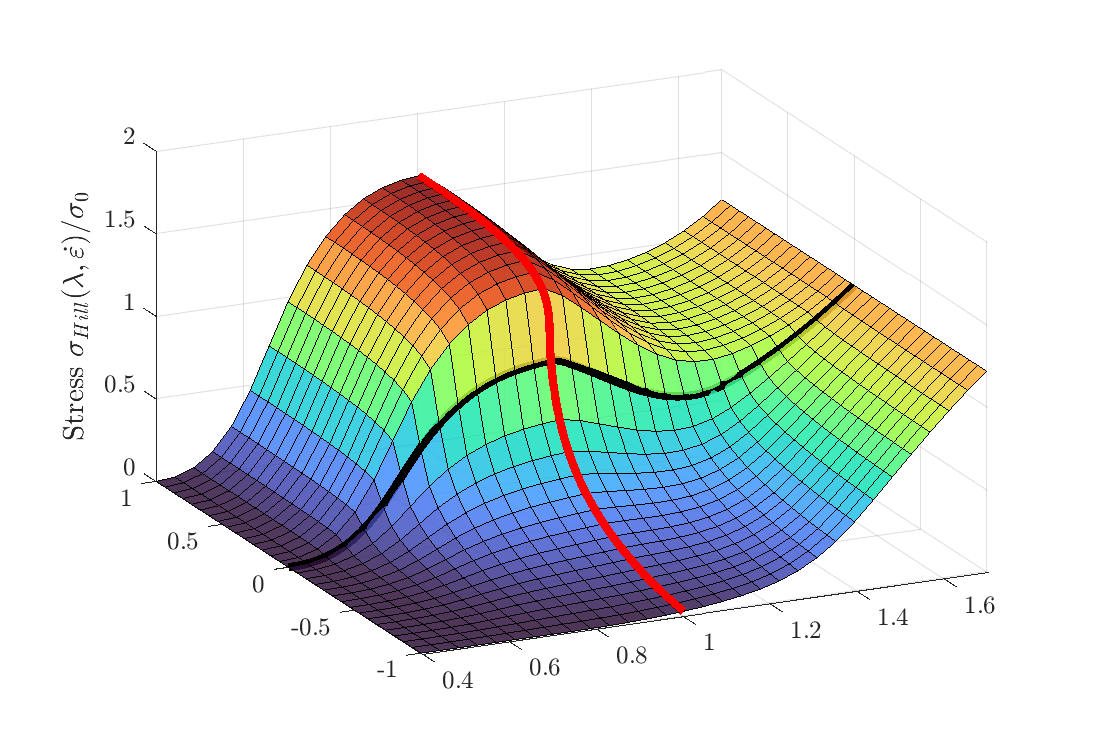
\includegraphics[width=0.85\textwidth]{plot_FLV_stress.eps}};
                %\node at (1.8,-1) [square,draw] {\large \phantom{A}};
                %\draw[->] (2.2, -1) -- (3.8,-0.8);
                \node[rotate=-35] at (-4.5,-3) {\small Fibre Strain Rate $\depsilon$};
                \node[rotate=8] at (2.4,-3.9) {\small Fibre Stretch $\lambda$};
            \end{tikzpicture}
    \caption{Hill's model depicted as a manifold in which the fibre stretch $\lambda$ and the fibre strain rate $\depsilon$ can vary simultaneously according to \eqref{eq:def_hill_stress_sigma}. We also show the curves $\sigma_{Hill}(\lambda,0)/\sigma_0$ (red) and $\sigma_{Hill}(0,\depsilon)/\sigma_0$ (black), which correspond to the total force-length (FL) and force-velocity (FV) relationships in Figure \ref{fig:plot_FL_FV}. \label{fig:plot_FLV}}
\end{figure}

{\color{red}We assume that the SEF $\Psi_{fibre}$ is given implicitly by the equation:}
\begin{equation} \label{eq:ode_fibre_sef}
    2 \I_4 \pder{\Psi_{fibre}}{\I_4} = \sigma_{Hill}(\bar{\lambda}, \bar{\depsilon}),
\end{equation}
where $\sigma_{Hill}$ is Hill's muscle model written in terms of the maximum isometric stress $\sigma_{0,mus}$:
\begin{equation} \label{eq:def_hill_stress_sigma}
    \sigma_{Hill}(\bar{\lambda}, \bar{\depsilon}) = \sigma_{0,mus} \left( a(\*X,t) \widehat{\sigma}_A(\bar{\lambda}) \widehat{\sigma}_V(\bar{\depsilon}) + \widehat{\sigma}_P(\bar{\lambda}) \right).
\end{equation}
{\color{blue}In this expression, the active stress-stretch relationship $\sigma_A$, the stress-strain rate relationship $\widehat{\sigma}_V$, and the passive stress-stretch relationship $\widehat{\sigma}_P$ can be taken exactly as the active force-length $F_V$, force-velocity $F_V$, and passive force-length $F_P$ relationships in \eqref{eq:Hill_force}, respectively (all these quantities are dimensionless, see Appendix \ref{app:force_relationships}). Furthermore, we now allow the activation function to also vary in space. For the special case when $a \equiv 1$, we portray this two-dimensional manifold in Figure \ref{fig:plot_FLV}.}

%\begin{figure}
%    \centering
%    \begin{tikzpicture}[square/.style={regular polygon,regular polygon sides=4}]
%        \node[inner sep=0pt] at (0,0)
%            {\hspace{-3.5em}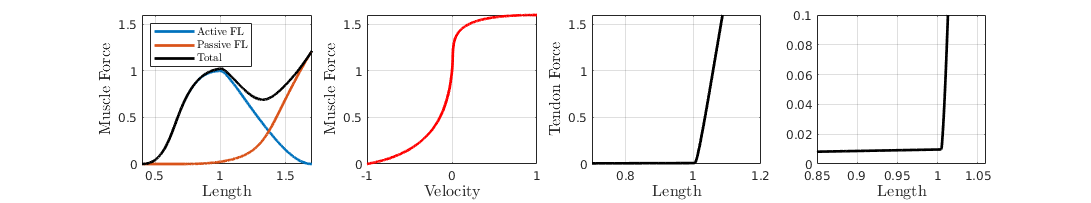
\includegraphics[width=1.18\textwidth]{force-curves-1D.png}};
%        \node at (1.8,-1) [square,draw] {\large \phantom{A}};
%        \draw[->] (2.2, -1) -- (3.8,-0.8);
%    \end{tikzpicture}
%    \caption{Force-relationships in use.}
%    \label{fig:force_curves_1D}
%\end{figure}

Using Equation \eqref{eq:def_S_bar}, the corresponding fictitious PK2 stress $\bar{\*S}_{fibre}$ can be computed as:
\begin{equation}
    \bar{\*S}_{fibre} = 2 \pder{\Psi_{fibre}}{\bar{\*C}} = 2 \pder{\Psi_{fibre}}{\I_4} \pder{\I_4}{\*C}.
\end{equation}
Thus, using \eqref{eq:ode_fibre_sef} together with \eqref{eq:derivatives_invariants}, we have:
\begin{equation} \label{eq:def_S_fibre}
    \bar{\*S}_{fibre} = \dfrac{1}{\bar{\lambda}^2} \sigma_{0,mus} \left( a(\*X,t) \widehat{\sigma}_A(\bar{\lambda}) \widehat{\sigma}_V(\bar{\depsilon}) + \widehat{\sigma}_P(\bar{\lambda}) \right) \*a_0(\*X) \otimes \*a_0(\*X),
\end{equation}
where $\*a_0$ is the initial orientation vector of a fibre crossing through the point $\*X \in \B_0$. Moreover, according to \eqref{eq:def_tau_bar}, we obtain that:
\begin{equation} \label{eq:def_tau_bar_fibre}
    \bar{\btau}_{fibre} = \dfrac{1}{\bar{\lambda}^2} \sigma_{0,mus} \left( a(\*X,t) \widehat{\sigma}_A(\bar{\lambda}) \widehat{\sigma}_V(\bar{\depsilon}) + \widehat{\sigma}_P(\bar{\lambda}) \right) \bar{\*a} \otimes \bar{\*a},
\end{equation}
where $\bar{\*a} := \bar{\*F}\*a_0$.

\subsection{Base material}

The base material component can be modelled using the following Yeoh SEF \cite{Paper3_RossEtAl2021, Paper2_RyanEtAl2020, Paper1_WakelingEtAl2020}:
\begin{equation}\label{eq:def_Psi_bm}
    \Psi_{bm}(\I_1) = s_{bm} \sigma_{0,bm} \sum_{k=1}^3 c_k (\I_1 - 3)^k,
\end{equation}
where $s_{bm}$ is a scaling factor, $\sigma_{0,bm}$ a normalizing constant stress, and $c_k \in \R$ are constants that were computed by Wakeling et al. \cite{Paper1_WakelingEtAl2020} to fit the experimental data in Mohammadkhah et al. \cite{Mohammadkhah2016}.

Similarly to the computation of $\bar{\*S}_{fibre}$ and $\bar{\btau}_{fibre}$, the fictitious PK2 and Kirchhoff stresses in this case are:
\begin{equation} \label{eq:def_S_bar_bm}
    \bar{\*S}_{bm} = s_{bm} \sigma_{0,bm} \left( 3c_3(\I_1-3)^2 + 2c_2 (\I_1-3) + c_1 \right) \*I,
\end{equation}
and
\begin{equation}
    \bar{\btau}_{bm} = s_{bm} \sigma_{0,bm} \left( 3c_3(\I_1-3)^2 + 2c_2 (\I_1-3) + c_1 \right) \bar{\*b}.
\end{equation}

In the work by Konno et al. \cite{KonnoNigamWakeling2021_ECM}, the base material is considered as a weighted combination of ECM and cellular material contributions to study muscle affected by cerebral palsy. More precisely, the expression for the SEF $\Psi_{bm}$ takes the form:
\begin{equation}
    \Psi_{bm}(\I_1) = \chi_{ecm} \Psi_{ecm}(\I_1) + (1-\chi_{ecm}) \Psi_{cell}(\I_1),
\end{equation}
where $\chi_{ecm} > 0$ is the fraction of ECM content in muscle. The SEFs for ECM and cellular material are given respectively by:
\begin{equation}\label{eq:def_Psi_ecm}
    \Psi_{ecm}(\I_1) = s_{ecm} \sum_{k=1}^3 c_k (\I_1 - 3)^k,
\end{equation}
and
\begin{equation}\label{eq:def_Psi_cell}
    \Psi_{cell}(\I_1) = s_{cell} \sum_{k=1}^3 c_k (\I_1 - 3)^k.
\end{equation}
The constants $c_k \in \R$ in these models have been computed by Konno et al. \cite{KonnoNigamWakeling2021_ECM} to fit the data in Gillies et al. \cite{Gillies2011} for the ECM and the data in Jin et al. \cite{Jin2013} for the cellular material.

In this case, the fictitious stress tensors for each one of these SEFs are given by:
\begin{gather}
    \bar{\*S}_{ecm} = s_{ecm} \left( 3c_3(\I_1-3)^2 + 2c_2 (\I_1-3) + c_1 \right) \*I, \\
    \bar{\btau}_{ecm} = s_{ecm} \left( 3c_3(\I_1-3)^2 + 2c_2 (\I_1-3) + c_1 \right) \bar{\*b},
\end{gather}
and
\begin{gather}
    \bar{\*S}_{cell} = s_{cell} \left( 3c_3(\I_1-3)^2 + 2c_2 (\I_1-3) + c_1 \right) \*I, \\
    \bar{\btau}_{cell} = s_{cell} \left( 3c_3(\I_1-3)^2 + 2c_2 (\I_1-3) + c_1 \right) \bar{\*b}.
\end{gather}

The constants $\sigma_{0,base}$, $s_{base}$, $s_{ecm}$, $s_{cell}$, as well as $c_k$ (which are local to each SEF), are given in Table \ref{tab:constants_base_material_muscle}. Note that the bulk modulus $\kappa$ used to define the volumetric component $\Psi_{vol}$ of the SEF $\Psi$ now takes the form
\begin{equation} \label{eq:def_kappa_ecm_cell}
    \kappa = \chi_{ecm} \kappa_{ecm} + (1-\chi_{ecm}) \kappa_{cell},
\end{equation}
where $\kappa_{ecm}$ and $\kappa_{cell}$ are the bulk moduli for ECM and cellular material, respectively.

\begin{table}
    \centering
    \begin{tabular}{|c|c|c|c|c|c|}\hline
        & Value in $\Psi_{bm}$ \eqref{eq:def_Psi_bm} & & Value in $\Psi_{ecm}$ \eqref{eq:def_Psi_ecm} & & Value in $\Psi_{cell}$ \eqref{eq:def_Psi_cell} \\\hline
        $\sigma_{0,bm}$ & 200000 \si{Pa} & - & - & - & - \\\hline
        $s_{bm}$ & 1 & $s_{ecm}$ & 200 \si{Pa} & $s_{cell}$ & 1 \si{Pa} \\\hline
        $c_1$ & 0.1990559575103343 & $c_1$ & 1988.76435209844 & $c_1$ & 3703.32723408173 \\\hline
        $c_2$ & 0.3662334826469149 & $c_2$ & 4917.02551347748 & $c_2$ & -707.76064007684 \\\hline
        $c_3$ & 0.0 & $c_3$ & -591.533166457473 & $c_3$ & 123.247643527575 \\\hline
    \end{tabular}
    \caption{Constants in the SEFs defining the base material component of muscle tissue.
    \label{tab:constants_base_material_muscle}}
\end{table}

\subsection{Intramuscular fat} \label{sec:intramuscular_fat}

\begin{table}
    \centering
    \begin{tabular}{|c|c|}\hline
        & Value in $\Psi_{fat}$ \eqref{eq:def_Psi_fat} \\\hline
        $s_{fat}$ & 1 \si{Pa} \\\hline
        $c_1$ & 323.91 \\\hline
        $c_2$ & 5163.1 \\\hline
        $c_3$ & -3872.9 \\\hline
    \end{tabular}
    \caption{Constants in the SEF defining intramuscular fat. \label{tab:constants_fat}}
\end{table}

Following \cite{KonnoEtAl2022_CP}, we consider the following SEF to model intramuscular fat:
\begin{equation} \label{eq:def_Psi_fat}
    \Psi_{fat}(\I_1) = s_{fat} \sum_{k=1}^3 c_k (\I_1 - 3)^k,
\end{equation}
where $s_{fat}$ is a scaling factor and the constants $c_k$ are computed so that the expression above fits the data by Alkhouli et al. \cite{Alkhouli2013}. The values for these constants are listed in Table \ref{tab:constants_fat}. Thus, the expressions for the fictitious stress tensors become:
\begin{equation}
    \bar{\*S}_{fat} = s_{fat} \left( 3c_3(\I_1-3)^2 + 2c_2 (\I_1-3) + c_1 \right) \*I, 
\end{equation}
and
\begin{equation}
    \bar{\btau}_{fat} = s_{fat} \left( 3c_3(\I_1-3)^2 + 2c_2 (\I_1-3) + c_1 \right) \bar{\*b}.
\end{equation}
The bulk modulus for the volumetric SEF $\Psi_{vol}$ now takes the form:
\begin{equation} \label{eq:def_kappa_bm_fat}
    \kappa = (1-\chi_{fat}) \kappa_{bm} + \chi_{fat} \kappa_{fat},
\end{equation}
where $\kappa_{bm}$ and $\kappa_{fat}$ are the bulk moduli for the base material and fat components. In particular, $\kappa_{bm}$ can be taken as a single constant or as the homogenized version in Equation \eqref{eq:def_kappa_ecm_cell}.

\section{Extending the SEF to the muscle-tendon unit} \label{sec:extension_sef_mtu}

The expressions in the previous section are only applicable to geometries made entirely of muscle tissue, without internal or external tendons. To create a SEF for the whole muscle-tendon unit, let us consider a partition of the domain of interest into three parts $\B_0 = \B_0^M \cup \B_0^A z \cup \B_0^T$, where $\B_0^M$, $\B_0^A$, and $\B_0^T$ represent the parts of $\B_0$ made of muscle tissue, aponeurosis, and tendon. Thus, a SEF for the MTU reads:
\begin{equation}
    \Psi_{MTU}(\*X,t) = \Psi_{mus}(\*X,t) \bm{\iota}_M(\*X) + \Psi_{apo}(\*X,t) \bm{\iota}_A(\*X) + \Psi_{ten}(\*X,t) \bm{\iota}_T(\*X),
\end{equation}
where $\bm{\iota}_M(\*X)$, $\bm{\iota}_A(\*X)$, and $\bm{\iota}_T(\*X)$ are indicator functions on $\B_0^M$, $\B_0^A$, and $\B_0^T$, respectively. Here, following Wakeling et al. \cite{Paper1_WakelingEtAl2020}, we consider an expression in common for the SEF of tendon and aponeurosis:
\begin{equation}
    \Psi_{tis} = \Psi_{vol,tis}(J) + \Psi_{iso,tis}(\I_1,\I_4), \quad tis \in \{apo,ten\}.
\end{equation}
Similar to muscle tissue, the volumetric part is given by
\begin{equation}
    \Psi_{vol,tis} = \dfrac{\kappa_{tis}}{4} \left( J^2 - 2\ln J - 1 \right), \quad tis \in \{apo,ten\},
\end{equation}
where $\kappa_{apo}$ and $\kappa_{ten}$ are the bulk moduli for aponeurosis and tendon, respectively. On the other hand, the isochoric component is given by:
\begin{equation}
    \Psi_{iso,tis} = \Psi_{tis,fibre}(\I_4) + \Psi_{tis,bm}(\I_4), \quad tis \in \{apo,ten\},
\end{equation}
as tendon and aponeurosis are also transversely-isotropic materials.

Assuming that the fibre component $\Psi_{tis,fibre}$ satisfies:
\begin{equation}
    2 \I_4 \pder{\Psi_{tis,fibre}}{\I_4} = \sigma_{0,tis} \widehat{\sigma}_{tis}(\bar{\lambda}), \quad tis \in \{apo,ten\},
\end{equation}
for a given stress-stretch relationship $\widehat{\sigma}_{tis}$ (see Appendix \ref{app:force_relationships}), we obtain the following stress tensors:
\begin{align}
    \bar{\*S}_{tis,fibre} &= \dfrac{1}{\bar{\lambda}^2} \sigma_{0,tis} \widehat{\sigma}_{tis}(\bar{\lambda}) \, \*a_0 \otimes \*a_0, \\
    \label{eq:def_tau_bar_tis_fibre}\bar{\btau}_{tis,fibre} &= \dfrac{1}{\bar{\lambda}^2} \sigma_{0,tis} \widehat{\sigma}_{tis}(\bar{\lambda}) \, \bar{\*a} \otimes \bar{\*a}.
\end{align}
Moreover, assuming that SEF for the base material $\Psi_{tis,bm}$ is given by a Yeoh SEF:
\begin{equation} \label{eq:def_Psi_tis_bm}
    \Psi_{tis,bm} = s_{tis} \sigma_{0,tis} \sum_{k=1}^3 c_k (\I_1 - 3)^k,
\end{equation}
we obtain the following stress tensors:
\begin{align}
    \bar{\*S}_{tis, bm} = 2 s_{tis} \sigma_{0,tis}  \left( 3c_3(\I_1-3)^2 + 2c_2 (\I_1-3) + c_1 \right) \*I, \\
    \label{eq:def_tau_bar_tis_bm}\bar{\btau}_{tis,bm} = 2 s_{tis} \sigma_{0,tis}  \left( 3c_3(\I_1-3)^2 + 2c_2 (\I_1-3) + c_1 \right) \bar{\*b}.
\end{align}
Following \cite{Seba} we assume that the constants $c_k$, $k=1,2,3$, are identical for tendon and aponeurosis. These have been fitted in \cite{Seba} from wild turkey gastrocnemii data \cite{Azizi2009} and are listed in Table \ref{tab:constants_ten_apo}.

\begin{table}
    \centering
    \begin{tabular}{|c|c|}\hline
        & Value in $\Psi_{tis}$ \eqref{eq:def_Psi_tis_bm} \\\hline
        $s_{tis}$ & 1 \\\hline
        $\sigma_{0,tis}$ & 200,000 \si{Pa} \\\hline
        $c_1$ & 4.6896264975 \\\hline
        $c_2$ & -3.45514101975 \\\hline
        $c_3$ & $4.8492055395 \cdot 10^2$ \\\hline
    \end{tabular}
    \caption{Constants in the SEF defining tendon and aponeurosis. \label{tab:constants_ten_apo}}
\end{table}

%Furthermore, the bulk modulus $\kappa$ takes the form
%\begin{equation}
%    \kappa(\*X) = \kappa_{muscle} \bchi_M(\*X) + \kappa_{apo} \bchi_A(\*X) + \kappa_{ten} \bchi_T(\*X),
%\end{equation}
%where $\kappa_{apo}$ and $\kappa_{tendon}$ are the bulk moduli for aponeurosis and tendon, respectively. In turn, $\kappa_{muscle}$ can be taken either as a single constant, or as a combination of the homogenized versions \eqref{eq:def_kappa_ecm_cell} and \eqref{eq:def_kappa_bm_fat}, that is
%\begin{equation}
%    \kappa_{muscle} = (1-\alpha) \left[ \beta \kappa_{ecm} + (1-\beta) \kappa_{cell} \right] + \alpha \kappa_{fat}.
%\end{equation}

%\subsection{Tendon and aponeurosis}

%Similar to muscle tissue, tendon and aponeurosis are made of dense fibrous connective tissues. However, 

%\begin{itemize}
%    \item SAME PROPERTIES (for tendon and aponeurosis) \cite{BlemkerDelp2005,BolReese2008}
%    \item DIFFERENT PROPERTIES \cite{Hadi}.
%    \item SAME STRUCTURE, PARAMETERS CAN VARY \cite{Seba}
%\end{itemize}

\section{Lagrangian formulation of the elastodynamic problem}

\begin{figure}
    \centering
    
\includegraphics[width=0.5\textwidth]{placeholder-img.jpg}
    \caption{Continuum representation of the muscle-tendon unit.\label{fig:continuum_mtu}}
\end{figure}

Let $\B_0 \subset \R^3$ be a region in three-dimensional space representing the undeformed muscle-tendon unit (MTU), potentially containing a combination of muscle, aponeurosis, and tendon, as described in Section \ref{sec:extension_sef_mtu}. The boundary of this body, $\partial \B_0$, can be subdivided into two parts: $\partial \B_0 = \Gamma_{0,D} \cup \Gamma_{0,N}$, with $\Gamma_{0,D} \cap \Gamma_{0,N} = \emptyset$. They represent respectively the Dirichlet and Neumann parts of the boundary in the reference configuration. Let also $\B_t$ denote the deformed MTU at time $t > 0$ (see Figure \ref{fig:continuum_mtu}).

The elastodynamic deformation of the MTU can be modelled using a system of PDEs in which, given an initial displacement $\*U_0 \in \*H^1(\B_0)$, an initial velocity $\*V_0 \in \*H^1(\B_0)$, an initial pressure $p_0 \in L^2(\B_0)$, a body force $\*f_0(\cdot, t) \in \*L^2(\B_0)$, a prescribed traction $\*T(\cdot,t) \in \*H^{-1/2}(\Gamma_{N,0})$, and a prescribed displacement $\*U_D(\cdot, t) \in \*H^{1/2}(\Gamma_{D,0})$, we want to find large (material) displacements $\*U(\cdot,t) \in \*H^1(\B_0)$, a (material) velocity $\*V \in \*H^1(\B_0)$, a (material) internal pressure $p(\cdot,t) \in L^2(\B_0)$, and a (material) dilation $D(\cdot, t) \in L^2(\B_0)$ such that:
\begin{subequations} \label{eq:LF_main_system}
    \begin{align}
        \label{eq:LF_main_system_1}\pder{\*U}{t} &= \*V  \quad \text{in } \B_0 \times (0,\infty),\\
        \label{eq:LF_main_system_2}\rho_0 \pder{\*V}{t} - \Divt{\*P(\*U,\*V,p,D)} &= \*f_0 \quad \text{in } \B_0 \times (0,\infty), \\
        \label{eq:LF_main_system_3}J(\*U) - D &= 0 \quad \text{in } \B_0 \times (0,\infty), \\
        \label{eq:LF_main_system_4}p-\Psi'_{vol}(D) &= 0 \quad \text {in } \B_0 \times (0,\infty), \\
        \*U &= \*U_D \quad \text{on } \Gamma_{D,0} \times (0,\infty), \\
        \label{eq:bc_traction_0}\*P(\*U,\*V,p,D) \*N &= \*T \quad \text{on }\Gamma_{N,0} \times (0,\infty), \\
        \*U = \*U_0, \quad \*V=\*V_0, \quad p=p_0, \quad D &= D_0 \quad \text{in } \B_0 \times \{t=0\}.
    \end{align}
\end{subequations}
Here, the first expression corresponds to the definition of the material velocity (see Remark \ref{re:velocity_def}), whereas the second equation is just Cauchy's first equation of motion written in the Lagrangian description (see \cite[Section 4.3]{HolzapfelBook}). 
The third equation is a constraint that relates $D$ to its definition.
Furthermore, $\rho_0$ denotes the \textit{reference density} of the MTU, and although it might depend on space coordinates $\*X$, it does not depend on time.

\begin{remark} \label{re:quasi-static_dynamic}
    The set of equations \eqref{eq:LF_main_system} corresponds to a dynamic extension of the Euler-Lagrange equations that arise from the stationarity of the potential first proposed by Simo et al. \cite{SimoTaylorPister1985}:
    \begin{equation} \label{eq:potential_qs}
        \Pi(\*U,p,D) = \int_{\B_0} \Psi_{vol}(D) + p(J(\*U) - D) + \Psi_{iso}(\bar{\*C}) - \int_{\B_0} \*f_0 \cdot \*U.
    \end{equation}
    Therefore, we refer to \eqref{eq:LF_main_system} as the \textit{dynamic} system. In turn, if we neglect the effect of the velocity on the system (i.e. $\*V \equiv 0$) as in \eqref{eq:potential_qs}, then we refer to \eqref{eq:LF_main_system} as the \textit{quasi-static} system.    
\end{remark}

We also note that the system \eqref{eq:LF_main_system_1}-\eqref{eq:LF_main_system_4} is equivalent to the Eulerian formulation developed by Dominguez \cite{Seba}:
\begin{subequations} \label{eq:EF_main}
    \begin{align}
    \label{eq:EF_1}\pder{\*u}{t} &= \*v  \quad \text{in } \B_t,\\
    \label{eq:EF_2}\pder{(\rho \*v)}{t} + \divt{(\rho \*v \otimes \*v)} - \divt{\bsigma(\*u,\*v,p,D)} &= \*f \quad \text{in } \B_t, \\
    \label{eq:EF_3}J(\*u)-D &= 0 \quad \text{in } \B_t, \\
    \label{eq:EF_4}p-\Psi'_{vol}(D) &= 0 \quad \text {in } \B_t,
    \end{align}
\end{subequations}
where the density in the current configuration $\rho$ is given by
\begin{equation}
    \rho = J(\*u)^{-1} \rho_0,
\end{equation}
and the body force $\*f$ is:
\begin{equation}
    \*f(\*x,t) = J(\*U)^{-1} \, \*f_0(\bm{\varphi}^{-1}(\*x,t),t).
\end{equation}
However, we have chosen to work with the Lagrangian formulation \eqref{eq:LF_main_system} because it leads to a simpler variational formulation, which consequently leads to a (significantly) simpler linearization of the problem (see below).

\section{A first order, fully implicit time discretization}

Based on the Neo-Hookean experiments we performed in Chapter \ref{ch:neohookean}, we discretize \eqref{eq:LF_main_system} using Rothe's method with a first-order, fully-implicit time stepping scheme. In this way, let us consider a time step size $\Delta t = T/N$ and time steps $t_n = n \Delta t$, with $n=0,\dots,N$ and $T > 0$ the simulation end time. For each $n \geq 0$, we seek approximations $\*U^{n+1}(\*X) \approx \*U(\*X,t^{n+1})$, $\*V^{n+1}(\*X) \approx \*V(\*X,t^{n+1})$, $p^{n+1}(\*X) \approx p(\*X,t^{n+1})$, and $D^{n+1}(\*X) \approx D(\*X,t^{n+1})$ such that:
\begin{subequations}
    \begin{align}
    \dfrac{\*U^{n+1} - \*U^n}{\Delta t} &= \*V^{n+1} \quad &&\text{in } \B_0, \\
    \rho_0 \dfrac{\*V^{n+1} - \*V^n}{\Delta t} - \Divt{\*P(\*U^{n+1}, \*V^{n+1}, p^{n+1}, D^{n+1})} &= \*f_0^{n+1} \quad &&\text{in } \B_0, \\
    J(\*U^{n+1}) - D^{n+1} &= 0 \quad &&\text{in } \B_0, \\
    p^{n+1}-\Psi'_{vol}(D^{n+1}) &= 0 \quad &&\text {in } \B_0, \\
    \label{eq:bc0_1} \*U^{n+1} &= \*U_D^{n+1} \quad &&\text{on } \Gamma_{D,0}, \\
    \label{eq:bc0_2} \*P(\*U^{n+1},\*V^n,p^{n+1},D^{n+1}) \*N &= \*T^{n+1} \quad &&\text{on }\Gamma_{N,0}.
    \end{align}
\end{subequations}
Combining the first two equations above we obtain the following displacement-pressure-dilation system: for each $n \geq 0$, find $\*U^{n+1}$, $p^{n+1}$, and $D^{n+1}$ such that:
\begin{subequations}\label{eq:LF_time}
    \begin{align}
    \label{eq:LF_time_1}\rho_0 \*U^{n+1} - \Delta t^2 \, \Divt{\*P(\*U^{n+1}, \*V^{n+1}, p^{n+1}, D^{n+1})} &= \rho_0 \*U^n + \Delta t \, \rho_0 \*V^n + \Delta t^2 \*f_0^{n+1}, \\
    \label{eq:LF_time_2}D^{n+1}-J(\*u^{n+1}) &= 0 , \\
    \label{eq:LF_time_3}p^{n+1}-\Psi'_{vol}(D^{n+1}) &= 0,
    \end{align}
\end{subequations}
and
\begin{equation}
    \*V^{n+1} = \dfrac{\*U^{n+1} - \*U^n}{\Delta t},
\end{equation}
with boundary conditions \eqref{eq:bc0_1} and \eqref{eq:bc0_2} 

We now construct a variational formulation for the system \eqref{eq:LF_time}. First, multiplying \eqref{eq:LF_time_1} by $\delta \*U \in \*H^1_0(\B_0)$ and integrating by parts, we obtain:
\begin{multline} \label{eq:weak0_1}
    \int_{\B_0} \rho_0 \*U^{n+1} \cdot \delta \*U + \Delta t^2 \int_{\B_0} \*P(\*U^{n+1},\*V^{n+1}) : \nabla_0(\delta \*U)  \\
    = \int_{\B_0} \rho_0 \*U^n \cdot \delta\*U + \Delta t \int_{\B_0} \rho_0 \*V^n \cdot \delta\*U + \Delta t^2 \int_{\B_0} \*f_0^{n+1} \cdot \delta\*U + \Delta t^2 \int_{\Gamma_{N,0}} \*T^{n+1} \cdot \delta \*U.
\end{multline}
Furthermore, we can use \eqref{eq:def_PK1} to rewrite the second term in the previous expression as:
\begin{multline*}
    \int_{\B_0} \*P(\*U^{n+1},\*V^{n+1}, p^{n+1}, D^{n+1}) : \nabla_0(\delta \*U) \\
    \begin{aligned}
        &= \int_{\B_0}  J(\*U^{n+1}) \, \bsigma(\*U^{n+1},\*V^n, p^{n+1}, D^{n+1}) : \nabla_0(\delta\*U) \*F(\*U^{n+1})^{-1} \\
        &= \int_{\B_0}  \btau(\*U^{n+1},\*V^n, p^{n+1}, D^{n+1}) : \nabla_0(\delta\*U) \*F(\*U^{n+1})^{-1}.
    \end{aligned}
\end{multline*}
Thus, we can rewrite \eqref{eq:weak0_1} as
\begin{multline} \label{eq:weak0_2}
\int_{\B_0} \rho_0 \*U^{n+1} \cdot \delta \*U + \Delta t^2 \int_{\B_0} \btau(\*U^{n+1},\*V^{n+1}) : \nabla_0(\delta\*U) \*F(\*U^{n+1})^{-1}  \\
= \int_{\B_0} \rho_0 \*U^n \cdot \delta\*U + \Delta t \int_{\B_0} \rho_0 \*V^n \cdot \delta\*U + \Delta t^2 \int_{\B_0} \*f_0^{n+1} \cdot \delta\*U + \Delta t^2 \int_{\Gamma_{N,0}} \*T^{n+1} \cdot \delta \*U. 
\end{multline}

Similarly, for equations \eqref{eq:LF_time_2} and \eqref{eq:LF_time_3}, we multiply them respectively by test functions $\delta p \in L^2(\B_0)$ and $\delta D \in L^2(\B_0)$ and integrate:
\begin{equation} \label{eq:weak_3}
    \int_{\B_0} \Big\{  J(\*U^{n+1}) - D^{n+1}  \Big\} \cdot \delta p = 0,
    \end{equation}
and
\begin{equation} \label{eq:weak_4}
    \int_{\B_0} \Big\{ \psi'_{vol}(D^{n+1}) - p^{n+1} \Big\} \cdot \delta D = 0.
\end{equation}

Finally, multiplying \eqref{eq:weak0_2} by $\Delta t^{-2}$ and adding it to \eqref{eq:weak_3} and \eqref{eq:weak_4}, we obtain the following nonlinear formulation of the semi-discrete problem \eqref{eq:LF_time}: find $\*U^{n+1} \in \*H^1(\B_0)$, $p^{n+1} \in L^2(\B_0)$, and $D^{n+1} \in L^2(\B_0)$ such that
\begin{equation} \label{eq:LF_weak}
    R(\*U^{n+1},p^{n+1},D^{n+1} ; \delta\*U, \delta p, \delta D) = 0,
\end{equation}
for any $\delta\*U \in \*H_0^1(\B_0)$, $\delta p \in L^2(\B_0)$, and $\delta D \in L^2(\B_0)$, where
\begin{align} \label{eq:def_R_LF}
    \notag R(\*U^{n+1},&p^{n+1},D^{n+1} ; \delta\*U, \delta p, \delta D) := \\
    \notag &\Delta t^{-2} \int_{\B_0} \rho_0 \*U^{n+1} \cdot \delta\*U + \int_{\B_0} \btau(\*U^{n+1},\*V^{n+1}, p^{n+1}, D^{n+1}) : \nabla_0(\delta\*U) \*F(\*U^{n+1})^{-1} \\
    \notag &+ \int_{\B_0} \Big\{ J(\*U^{n+1}) - D^{n+1} \Big\} \cdot \delta p + \int_{\B_0} \Big\{ \psi'_{vol}(D^{n+1}) - p^{n+1} \Big\} \cdot \delta D \\
    \notag &- \Delta t^{-1} \int_{\B_0} \rho_0 \*V^n \cdot \delta\*U - \Delta t^{-2} \int_{\B_0} \rho_0 \*U^n \cdot \delta \*U - \int_{\Gamma_{N,0}} \*T^{n+1} \cdot \delta\*U \\
    &- \int_{\B_0} \*f_0^{n+1} \cdot \delta \*U.
\end{align}

We may also refer to \eqref{eq:LF_weak} as the (semi-discretized) \textit{principle of virtual work} \cite{HolzapfelBook}. In particular, we may split $R$ into three components:
\begin{equation}
    R = R_{ine} + R_{int} - R_{ext},
\end{equation}
where the (semi-discrete) work due to inertial, internal, and external forces are respectively given by:
\begin{align}
    \notag R_{ine}(\*U^{n+1} ; \delta\*U) &= \Delta t^{-2} \int_{\B_0} \rho_0 \*U^{n+1} \cdot \delta\*U \\
    \notag &- \Delta t^{-2} \int_{\B_0} \rho_0 \*U^n \cdot \delta\*U \\
    \label{eq:def_Rine}&- \Delta t^{-1} \int_{\B_0} \rho_0 \*V^n \cdot \delta\*U,
\end{align}
\begin{align}
    \notag R_{int}(\*U^{n+1}, p^{n+1}, D^{n+1} ; \delta\*U, \delta p, \delta D) &= \int_{\B_0} \btau^{n+1} : \nabla_0(\delta\*U) \*F(\*U^{n+1})^{-1} \\
    \notag &+ \int_{\B_0} \Big\{ J(\*U^{n+1}) - D^{n+1} \Big\} \cdot \delta p \\
    \label{eq:def_Rint}&+ \int_{\B_0} \Big\{ \psi'_{vol}(D^{n+1}) - p^{n+1} \Big\} \cdot \delta D,
\end{align}
and
\begin{equation}
    \label{eq:def_Rext}R_{ext}(\delta \*U) =  \int_{\Gamma_{N,0}} \*T^{n+1} \cdot \delta\*U + \int_{\B_0} \*f_0^{n+1}  \cdot \delta\*U.
\end{equation}
In Equation \eqref{eq:def_Rint}, we have written $\btau^{n+1} = \btau(\*U^{n+1},\*V^{n+1}, p^{n+1}, D^{n+1})$.

\begin{remark}
    Using this notation, a variational formulation for the quasi-static problem that arises from \eqref{eq:LF_main_system} (or equivalently, the stationarity of the potential \eqref{eq:potential_qs}) reads: find $\*U^{n+1} \in \*H^1(\B_0)$, $p^{n+1} \in L^2(\B_0)$, and $D^{n+1} \in L^2(\B_0)$ such that
    \begin{equation}
        R_{int}(\*U^{n+1}, p^{n+1}, D^{n+1} ; \delta\*U, \delta p, \delta D) = R_{ext}(\delta \*U),
    \end{equation} 
    for all virtual displacements $\delta\*U \in \*H_0^1(\B_0)$, virtual pressures $\delta p \in L^2(\B_0)$, and virtual dilations $\delta D \in L^2(\B_0)$. Recall that, in this case, the equations do not involve
\end{remark}

Before jumping into the linearization of the nonlinear problem \eqref{eq:LF_weak}, let us see how this formulation differs from the one introduced in \cite{Seba}.

\begin{remark}
    Consider the variational formulation for the Eulerian system \eqref{eq:EF_main} as in \cite[Equation 6.22]{Seba} pulled back to the reference configuration: find $\*U^{n+1} \in \*H^1(\B_0)$, $p^{n+1} \in L^2(\B_0)$, and $D^{n+1} \in L^2(\B_0)$ such that
    \begin{equation} \label{eq:EF_weak}
        \widetilde{R}(\*U^{n+1},p^{n+1},D^{n+1} ; \delta\*U, \delta p, \delta D) = 0,
    \end{equation}
    for any $\delta\*U \in \*H_0^1(\B_0)$, $\delta p \in L^2(\B_0)$, and $\delta D \in L^2(\B_0)$, where
    \vspace*{-0.5em}
    \begin{align} \label{eq:def_R_EF}
        \notag \widetilde{R}(\*U^{n+1},&p^{n+1},D^{n+1} ; \delta\*U, \delta p, \delta D) := \\
        \notag &\Delta t^{-2} \int_{\B_0} \rho_0 \*U^{n+1} \cdot \delta \*U + \int_{\B_0} \btau(\*U^{n+1},\*V^n, p^{n+1}, D^{n+1}) : \nabla^S_0(\delta\*U) \, \*F(\*U^{n+1})^{-1} \\
        \notag &+ \int_{\B_0} \Big\{  J(\*U^{n+1}) - D^{n+1} \Big\} \cdot \delta p + \int_{\B_0} \Big\{ \psi'_{vol}(D^{n+1}) - p^{n+1} \Big\} \cdot \delta D  \\
        \notag &- \Delta t^{-1} \int_{\B_0} \rho_0 \dfrac{J(\*U^{n+1})}{J(\*U^{n})} \*V^n \cdot \delta\*U \\
        \notag &-\int_{\B_0} \left(\rho_0 \dfrac{J(\*U^{n+1})}{J(\*U^{n})} \*V^n \otimes \*V^n\right) : \nabla^S_0(\delta \*U) \, \*F(\*U^{n+1})^{-1} \\
        \notag &+ \int_{\Gamma_{N,0}}  \left(\rho_0 \dfrac{J(\*U^{n+1})}{J(\*U^{n})} \*V^n \otimes \*V^n \right) \*F(\*U^{n+1})^{-T} \*N \cdot \delta \*U \\
        &- \Delta t^{-2} \int_{\B_0} \rho_0 \*U^n \cdot \delta \*U - \int_{\Gamma_{N,0}} \*T^{n+1} \cdot \delta\*U - \int_{\B_0} \*f_0^{n+1} \cdot \delta \*U.
    \end{align}
    Given that the Eulerian and the Lagrangian formulations model the exact same biological system but in difference frames of reference, it is clear that the nonlinear weak formulations \eqref{eq:LF_weak} and \eqref{eq:EF_weak} are completely equivalent. However, the linearization for these problems involves the computation of derivatives with respect to $\*U^{n+1}$, $p^{n+1}$, and $D^{n+1}$ for the first four terms in \eqref{eq:def_R_LF}, as opposed to the first seven in \eqref{eq:def_R_EF}. Furthermore, the weak problem \eqref{eq:LF_weak} represents a departure from \eqref{eq:EF_weak} since we are now treating the velocity implicitly in the Kirchhoff stress $\btau$, as opposed to the explicit treatment in \eqref{eq:def_R_EF} (as seen in the second term that defines $\widetilde{R}$).
\end{remark}

\section{Linearization}

The linearization of the three-field formulation \eqref{eq:LF_weak} is based on previous developments by Dominguez \cite{Seba} and Pelteret \cite{PelteretThesis}, with additional terms appearing naturally from the inertia of the system. First, we give general details of Newton iteration, along with the boundary conditions needed each for each iterate. Then, we provide computable versions of each one of the blocks that form the tangent operator $\bm{\mathcal{D}}R$.
%Finally, we focus on the computation of the fibre contribution to the fourth-order tensor $J\c$ since it is an expression that is typically not reported in the literature. In particular, we provide details on the treatment of the newton iterates for the along-fibre strain rate, rate of deformation tensor, and some derivatives of these quantities.

\subsection{Newton's method} \label{sec:newton_method}

Given $\*U^n$, $\*V^n$, $\*U^{n+1}_k$, $p^{n+1}_k$, and $D^{n+1}_k$, we want to find updates $\*d \*U_k$, $d p_k$, and $d D_k$ such that:
\begin{multline} \label{eq:newton}
    \quad \bm{\mathcal{D}}R(\*U^{n+1}_k, p^{n+1}_k, D^{n+1}_k) \Big(d \*U_k, d p_k, d D_k ; \delta \*U, \delta p, \delta D \Big) \\
    = - R(\*U^{n+1}_k, p^{n+1}_k, D^{n+1}_k ; \delta \*U, \delta p, \delta D), \quad
\end{multline}
for all virtual increments $\delta \*U$, $\delta p$, and $\delta D$, then update the solution as
\begin{equation} \label{eq:update_theory}
\*U^{n+1}_{k+1} = \*U^{n+1}_k + \*d \*U_k, \quad 
p^{n+1}_{k+1} = p^{n+1}_k + d p_k, \quad 
D^{n+1}_{k+1} = D^{n+1}_k + d D_k,
\end{equation}
until a convergence criterion is satisfied. Here, $\bm{\mathcal{D}} R$ denotes the G\^{a}teaux derivative of the operator $R$ ($\bm{\mathcal{D}} R$ is also known as the \textbf{tangent operator}). At the current time step, we set the initial solution as the converged one from the previous time step, i.e.,
\begin{equation}
\*U_0^{n+1} = \*U^n,
\end{equation}
with analogous expressions for the pressure and dilation. Therefore, the solution can be updated as:
\begin{equation} \label{eq:update_practice}
\*U^{n+1}_{k+1} = \*U^{n+1}_k + \*d\*U_k = \*U^{n+1}_{k-1} + \*d\*U_{k-1} + \*d \*U_k = \dots = \*U_0^{n+1} + \Delta \*U_k = \*U^n + \Delta \*U_k,
\end{equation}
where we have defined the object:
\begin{equation}
\Delta \*U_k = \sum_{l = 0}^k \*d \*U_k.
\end{equation}

\begin{remark}
Computationally speaking, at the beginning of every time step, one would set the object $\Delta \*U_k$ to zero and then start updating recursively this quantity with each Newton step $\*d \*U_k$. Then, once convergence has been achieved, we can obtain the converged solution for the current time step as in the last equality of \eqref{eq:update_practice}. This approach turns out to be less prone to numerical (round off) errors than updating the solution directly as in \eqref{eq:update_theory}.
\end{remark}

\begin{remark}[Boundary conditions for the linearized system]
    Consistent with the variational problem \eqref{eq:LF_weak}, the linearized problem \eqref{eq:newton} requires boundary conditions for the displacements $\*d \*U_k$ at each iteration $k$. To determine these, let us assume that for the time step $t_{n+1}$, the method converges in $K+1$ iterations. Thus, we can set $\*U^{n+1} := \*U_{K+1}^{n+1}$ and therefore, according to \eqref{eq:update_practice},
    \[
    \Delta \*U_K = \*d\*U_0 + \*d\*U_1 + \dots + \*d\*U_K = \*U^{n+1} - \*U^n.
    \]
    However, the displacements $\*U^{n+1}$ and $\*U^n$ are known along the Dirichlet part of the boundary. This suggests that, on $\Gamma_{0,D}$, we can set
    \begin{equation}
    \begin{aligned}
    \*d\*U_0 &= \*U^{n+1} - \*U^n, \\
    \*d\*U_1 &= \*0,  \\
    &\hspace{0.6em}\vdots \\
    \*d\*U_K &= \*0,
    \end{aligned}
    \end{equation}
    that is, the incremental displacement $\*U^{n+1}-\*U^n$ is only implemented at the first Newton iteration and zero Dirichlet boundary conditions can be assumed for the rest.
\end{remark}

\subsection{Construction of the block-matrix system}

We begin populating the elements forming the tangent operator $\bm{\mathcal{D}} R$ by computing the G\^{a}teaux derivatives of each relevant term in \eqref{eq:LF_weak}. First, for the inertial contribution, only the first term in \eqref{eq:def_Rine} depends on the current displacement, so the linearization of this term yields:
\begin{equation}
    \*K_{ine}^{\delta \*U, \*d \*U} = \der{}{\epsilon}R_{ine}(\*U_k^{n+1} + \epsilon \*d\*U_k ; \delta\*U) \Big|_{\epsilon = 0} = \Delta t^{-2} \int_{\B_0} \rho_0 \, \*d\*U_k \cdot \delta \*U.
\end{equation}

Next, for the internal contribution, the linearization of the first term in \eqref{eq:def_Rint} is discussed in general terms in \cite[Chapter 8]{HolzapfelBook}. This yields the term:
\begin{equation} \label{eq:def_K_int_11}
    \*K_{int}^{\delta \*U, \*d \*U} = \int_{\B_0} \nabla (\delta \*U) : J\c^{n+1}_k : \nabla(\*d\*U_k) + \int_{\B_0} \nabla(\delta \*U) : \nabla (\*d\*U_k) \btau^{n+1},
\end{equation}
where $\c^{n+1}_k = \c(\*U^{n+1}_k, \*V^{n+1}_k, p^{n+1}_k, D^{n+1}_k)$ is the fourth-order elasticity tensor defined in \eqref{eq:def_c_spatial}. The computation of this tensor will be the main focus of Section \ref{sec:elasticity_tensors}.

The rest of the contributions with respect to virtual displacements are easier to compute. Following \eqref{eq:def_tau}, we use the decomposition 
\begin{equation}
    \btau = \btau_{vol}(p,J(\*U)) + \btau_{iso}(\*U,\*V),
\end{equation}
as the pressure only appears in the volumetric part of the Kirchhoff stress and there is no dependence on the approximate dilation $D$:
\begin{equation}
\begin{aligned}
\*K^{\delta \*U, dp} &= \der{}{\epsilon} R_{int}(\*U^{n+1}_k, p^{n+1}_k + \epsilon dp_k, D^{n+1}_k; \delta\*U) \Big|_{\epsilon=0} \\
&= \int_{\B_0} dp_k J \, \*I : \nabla(\delta\*U) \\
&= \int_{\B_0} dp_k J \, \*I : \Big\{ \nabla_0(\delta\*U) \*F(\*U^{n+1}_k)^{-1} \Big\}
\end{aligned},
\end{equation}
and $\*K^{\delta\*U, dD} = 0$. Next, for the contributions with respect to virtual pressures, we have
\begin{equation}
\begin{aligned}
\*K^{\delta p, \*d\*U} &= \der{}{\epsilon} R_{int}(\*U^{n+1}_k + \epsilon \*d\*U_k, p^{n+1}_k, D^{n+1}_k ; \delta p) \Big|_{\epsilon=0} \\
&= \int_{\B_0} \delta p J \, \*I : \nabla (\*d\*U_k) \\
&= \int_{\B_0} \delta p J \, \*I : \Big\{ \nabla_0 (\*d\*U_k) \*F(\*U^{n+1}_k)^{-1} \Big\},
\end{aligned}
\end{equation}
$\*K^{\delta p, dp} = 0$, and
\begin{equation}
\begin{aligned}
\*K^{\delta p, dD} &= \der{}{\epsilon}R_{int}(\*U^{n+1}_k, p^{n+1}_k, D^{n+1}_k + \epsilon dD_k ; \delta p) \Big|_{\epsilon=0} \\
&= - \int_{\B_0} dD \, \delta p.
\end{aligned}
\end{equation}
Finally, for the contributions with respect to virtual dilations, we have $\*K^{\delta D, \*d\*U} = 0$, 
\begin{equation}
\begin{aligned}
\*K^{\delta D, dp} &= \der{}{\epsilon} R_{int}(\*U^{n+1}_k, p^{n+1}_k + \epsilon dp_k, D^{n+1}_k; \delta D) \Big|_{\epsilon=0}  \\
&= -\int_{\B_0}  dp \, \delta D,
\end{aligned}
\end{equation}
and
\begin{equation}
\begin{aligned}
\*K^{\delta D, dD} &= \der{}{\epsilon}R_{int}(\*U^{n+1}_k, p^{n+1}_k, D^{n+1}_k + \epsilon dD_k ; \delta D) \Big|_{\epsilon=0} \\
&= \int_{\B_0} \Psi_{vol}''(D^{n+1}_k) \, dD \, \delta D.
\end{aligned}
\end{equation}

Therefore, the problem \eqref{eq:newton} can formally be written in matrix form as:
\begin{equation} \label{eq:LF_linear_system}
    \left[\begin{matrix}
    \*K_{ine}^{\delta \*U, \*d\*U} + \*K_{int}^{\delta \*U, \*d\*U} & \*K^{\delta \*U, dp} & \*0 \\
    \*K^{\delta p, \*d\*U} & \*0 & \*K^{\delta p, dD} \\
    \*0 & \*K^{\delta D, dp} & \*K^{\delta D, dD}
    \end{matrix}\right] 
    \left( \begin{matrix}
      d\*U_k \\ dp_k \\ dD_k
    \end{matrix}\right) = -
    \left(\begin{matrix}
      R_{ine}(\*U^{n+1}_k) + R_{int}(\*U^{n+1}_k) \\
      R_{int}(p^{n+1}_k)\\
      R_{int}(D^{n+1}_k)
    \end{matrix}\right).
\end{equation}

\section{Fourth-order elasticity tensors} \label{sec:elasticity_tensors}

To compute the fourth-order tensor $\c^{n+1}$, we first need to find the material tensor $\bar{\C}$ (see Equations \eqref{eq:def_c}, \eqref{eq:Jc_iso}, and \eqref{eq:def_c_bar}). In fact, each contribution to the isochoric SEF $\Psi_{iso}$ yields a different contribution to the tensor $\bar{\C}$. For example, if we assume that $\B_0$ contains muscle fibres, base material, and intramuscular fat as in \eqref{eq:def_Psi_iso_fibre_bm_fat}, we will have:
\begin{equation}
    \bar{\C} = (1-\chi_{fat})(\bar{\C}_{fibre} + \bar{\C}_{bm}) + \chi_{fat} \bar{\C}_{fat},
\end{equation}
with analogous expressions if ECM, cell, tendon, or aponeurosis tissues are included. 

The derivation of all parts that make the $\bar{\C}$ tensor follows the same structure, so we focus mostly on the fibre contribution, as this is novel to the elastodynamics of skeletal muscle tissue. 

\subsection{Along-fibre contribution}

Because of the implicit treatment of the velocity in the Kirchhoff stress, and because we are not considering the velocity and displacement as \textit{independent} variables, the elasticity tensors needed for a Newton iteration take a more involved form (compared to the quasi-static case) that requires some particular approximations, specially regarding the modified fibre strain rate $\bar{\depsilon}$. This will be one of the main contributions in this section.

According to Equation \eqref{eq:def_C_bar}, we first have:
\begin{equation}
    J^{4/3} \bar{\C}_{fibre}^{n+1} = 2 \pder{\bar{\*S}_{fibre}^{n+1}}{\bar{\*C}^{n+1}} = 2 \pder{\bar{\*S}_{fibre}^{n+1}}{\I_4^{n+1}} \otimes \pder{\I_4^{n+1}}{\bar{\*C}^{n+1}}.
\end{equation}
Moreover, using \eqref{eq:derivatives_invariants} and the particular expression for $\bar{\*S}_{fibre}$ in \eqref{eq:def_S_fibre}, we obtain:
\begin{align}
    \notag J^{4/3} \bar{\C}_{fibre}^{n+1} &= 2 \pder{}{\I_4^{n+1}} \left[ \dfrac{1}{\I_4^{n+1}} \sigma_{Hill}(\I_4^{n+1})\right] \*a_0 \otimes \*a_0 \otimes \*a_0 \otimes \*a_0 \\
    &= 2 \left[ -\dfrac{1}{\left(\I_4^{n+1}\right)^2} \sigma_{Hill}(\I_4^{n+1}) + \dfrac{1}{\I_4^{n+1}} \pder{\sigma_{Hill}(\I_4^{n+1})}{\I_4^{n+1}} \right] \*a_0 \otimes \*a_0 \otimes \*a_0 \otimes \*a_0
\end{align}
At this juncture, we emphasize that these expressions are meant to be evaluated at the current Newton iteration $k$ (see \eqref{eq:def_K_int_11}). In particular, using the definition of Hill's fibre stress in \eqref{eq:def_hill_stress_sigma}, we obtain the following expression for its derivative:
\begin{align}
    \notag \pder{\sigma_{Hill}(\I_4^{n+1})}{\I_4^{n+1}} &= \pder{\sigma_{Hill}(\bar{\lambda}^{n+1}_k, \bar{\depsilon}^{n+1}_k)}{\bar{\lambda}^{n+1}_k} \pder{\bar{\lambda}^{n+1}_k}{\I_4^{n+1}} +  \pder{\sigma_{Hill}(\bar{\lambda}^{n+1}_k, \bar{\depsilon}^{n+1}_k)}{\bar{\depsilon}^{n+1}_k} \pder{\bar{\depsilon}^{n+1}_k}{\bar{\lambda}^{n+1}_k} \pder{\bar{\lambda}^{n+1}_k}{\I_4^{n+1}} \\
    \notag &= \sigma_{0,mus} \left[ a^{n+1} \der{\widehat{\sigma}_L(\bar{\lambda}^{n+1}_k)}{\bar{\lambda}^{n+1}_k} \widehat{\sigma}_V(\bar{\depsilon}^{n+1}_k) + \der{\widehat{\sigma}_P(\bar{\lambda}^{n+1}_k)}{\bar{\lambda}^{n+1}_k} \right] \dfrac{1}{2\bar{\lambda}^{n+1}_k} \\
    &\hspace{8em}+ \sigma_{0,mus} a^{n+1} \widehat{\sigma}_L(\bar{\lambda}^{n+1}_k) \der{\sigma_{V}(\bar{\depsilon}^{n+1}_k)}{\bar{\depsilon}^{n+1}_k} \pder{\bar{\depsilon}^{n+1}_k}{\bar{\lambda}^{n+1}_k} \dfrac{1}{2\bar{\lambda}^{n+1}_k}.
\end{align}

In particular, following the definition of the modified strain rate $\bar{\depsilon}$ in \eqref{eq:def_strain_rate_bar}$_2$ we consider:
\begin{equation} \label{eq:strain_rate_bar_newton_iteration}
    \bar{\depsilon}^{n+1}_k = \dfrac{1}{\depsilon_0} \dfrac{(\bar{\*F}_k^{n+1}\*a_0)^\T (\p : \*d^{n+1}_k) (\bar{\*F}_k^{n+1} \*a_0)}{\bar{\lambda}^{n+1}_k},
\end{equation}
where, according to \eqref{eq:def_l_spatial_velocity_gradient},
\begin{equation}
    \*d_k^{n+1} = \mathrm{symm} \left( \dfrac{\*F_k^{n+1} - \*F^n}{\Delta t} \left(\*F_k^{n+1}\right)^{-1} \right).
\end{equation}
However, for the term $\pder{\bar{\depsilon}^{n+1}_k}{\bar{\lambda}^{n+1}_k}$ (and only for this term), we approximate $\bar{\depsilon}^{n+1}_k$ as in \eqref{eq:def_strain_rate_bar}$_1$:
\begin{equation}
    \bar{\depsilon}^{n+1}_k \approx \dfrac{1}{\depsilon_0} \dfrac{\bar{\lambda}^{n+1}_k - \bar{\lambda}^n}{\Delta t},
\end{equation}
and thus we set:
\begin{equation} \label{eq:d_strain_rate_bar_d_lambda_bar}
    \pder{\bar{\depsilon}^{n+1}_k}{\bar{\lambda}^{n+1}_k} = \dfrac{1}{\depsilon_0} \dfrac{1}{\Delta t}.
\end{equation}

Therefore, the full expression for $J^{4/3} \bar{\C}_{fibre}^{n+1}$ reads:
\begin{equation}
    \notag J^{4/3} \bar{\C}_{fibre}^{n+1} = \mathfrak{C}\left(\bar{\lambda}^{n+1}_k, \bar{\depsilon}^{n+1}_k \right) \, \*a_0 \otimes \*a_0 \otimes \*a_0 \otimes \*a_0,
\end{equation}
where
\begin{align}
    \notag \mathfrak{C}\left(\bar{\lambda}^{n+1}_k, \bar{\depsilon}^{n+1}_k \right) = &- \dfrac{2}{\left( \bar{\lambda}^{n+1}_k \right)^4} \, \sigma_{0,mus} a^{n+1} \widehat{\sigma}_L(\bar{\lambda}^{n+1}_k) \widehat{\sigma}_V(\bar{\depsilon}^{n+1}_k) \\
    \notag &+ \dfrac{1}{\left( \bar{\lambda}^{n+1}_k \right)^3} \, \sigma_{0,mus} a^{n+1} \der{\widehat{\sigma}_L}{\bar{\lambda}} \left( \bar{\lambda}^{n+1}_k \right) \widehat{\sigma}_V(\bar{\depsilon}^{n+1}_k) \\
    \notag &+ \dfrac{1}{\left( \bar{\lambda}^{n+1}_k \right)^3} \, \sigma_{0,mus} a^{n+1} \widehat{\sigma}_L(\bar{\lambda}^{n+1}_k) \der{\widehat{\sigma}_V}{\bar{\depsilon}} \left( \bar{\depsilon}^{n+1}_k \right) \dfrac{1}{\depsilon_0 \Delta t} \\
    &- \dfrac{2}{\left( \bar{\lambda}^{n+1}_k \right)^4} \, \sigma_{0,mus} \widehat{\sigma}_P(\bar{\lambda}^{n+1}_k) + \dfrac{1}{\left( \bar{\lambda}^{n+1}_k \right)^3} \, \sigma_{0,mus} \der{\widehat{\sigma}_P}{\bar{\lambda}} \left( \bar{\lambda}^{n+1}_k  \right)
\end{align}
In this way,
\begin{equation}
    \bar{\c}_{fibre}^{n+1} = \mathfrak{C}\left(\bar{\lambda}^{n+1}_k, \bar{\depsilon}^{n+1}_k \right) \, \bar{\*a}_k^{n+1} \otimes \bar{\*a}_k^{n+1} \otimes \bar{\*a}_k^{n+1} \otimes \bar{\*a}_k^{n+1},
\end{equation}
where $\bar{\*a}_k^{n+1} = \bar{\*F}_k^{n+1} \*a_0$.

\begin{remark}
    If the simulation is quasi-static, then Hill's stress does not depend on the fibre strain rate, and therefore
    \begin{equation}
        \bar{\c}_{fibre}^{n+1} = \widetilde{\mathfrak{C}} \left(\bar{\lambda}^{n+1}_k \right) \, \bar{\*a} \otimes \bar{\*a} \otimes \bar{\*a} \otimes \bar{\*a},
    \end{equation}
    where
    \begin{align}
        \notag \widetilde{\mathfrak{C}} \left(\bar{\lambda}^{n+1}_k \right) = &-\dfrac{2\sigma_{0,mus}}{(\bar{\lambda}^{n+1}_k)^4} \, \left[ a^{n+1} \widehat{\sigma}_A(\bar{\lambda}^{n+1}_k)  + \widehat{\sigma}_P(\bar{\lambda}^{n+1}_k) \right] \\
        &+ \dfrac{\sigma_{0,mus}}{(\bar\lambda^{n+1}_k)^3} \Bigg[ a^{n+1} \der{\widehat{\sigma}_A}{\bar\lambda}\left(\bar\lambda^{n+1}_k\right) + \der{\widehat{\sigma}_P}{\bar{\lambda}}\left(\bar\lambda^{n+1}_k\right) \Bigg]
    \end{align}
\end{remark}

{\color{blue}
Although the expressions for the modified strain rate \eqref{eq:strain_rate_bar_newton_iteration} and its derivative with respect to the modified stretch \eqref{eq:d_strain_rate_bar_d_lambda_bar} may seem like a minor detail in the discretization of the Lagrangian formulation \eqref{eq:LF_main_system}, they constitute elements of the numerical method that can ``make or break'' the code for fully active, fully dynamic simulations. First, Dominguez \cite{Seba} suggested the following expression for the fibre strain rate:
\begin{equation}
    \bar{\depsilon}_k^{n+1} = \*V^n \cdot (\bar{\*F}_k^{n+1} \*a_0),
\end{equation}
with no information about what the expression for $\partial_{\bar{\lambda}_k^{n+1}} \bar{\depsilon}_k^{n+1}$ should look like. Later, in Ross et al. \cite{Paper3_RossEtAl2021}, the following expressions were used:
\begin{equation}
    \bar{\depsilon}_k^{n+1} = \dfrac{(\bar{\*F}^{n}\*a_0)^\T (\p : \*d^{n}) (\bar{\*F}^{n} \*a_0)}{\bar{\lambda}^{n+1}_k}, \quad \pder{\bar{\depsilon}_k^{n+1}}{\bar{\lambda}_k^{n+1}} = -\dfrac{\bar{\depsilon}_k^{n+1}}{\bar{\lambda}_k^{n+1}},
\end{equation}
with the latter being an expression that implicitly assumes that the strain rate $\bar{\depsilon}_k^{n+1}$ does depend on the current deformation tensor $\bar{\*F}_k^{n+1}$ in the numerator, but keeps the deviatoric part of the rate of strain tensor (i.e. $\p:\*d^n$) constant for the current time step and the current Newton iteration. While this work does contain fully active, fully dynamic contractions, Tam \cite{Cassidy} would later find that the FV properties in this work where not implemented properly, as any contraction would lead to the strain-rate-dependent stress $\widehat{\sigma}_V(\depsilon)$ in \eqref{eq:def_hill_stress_sigma} default to its maximum value of 1.5950. To remediate this, Tam \cite{Cassidy} made use of the following expressions:
\begin{equation}
    \bar{\depsilon}_k^{n+1} = \dfrac{(\bar{\*F}_k^{n+1}\*a_0)^\T (\p : \*d^{n}) (\bar{\*F}_k^{n+1} \*a_0)}{\bar{\lambda}^{n+1}_k}, \quad \pder{\bar{\depsilon}_k^{n+1}}{\bar{\lambda}_k^{n+1}} = +\dfrac{\bar{\depsilon}_k^{n+1}}{\bar{\lambda}_k^{n+1}}.
\end{equation}
This resulted in successful dynamic contractions but only to a maximum of 50\% activation, provided the following time size restriction is met:
\begin{equation}
    \dfrac{c \Delta t}{h} < 1, \quad c := \sqrt{\dfrac{\kappa}{\rho_0}}.
\end{equation}
}

\subsection{Base material and other components of the MTU}

Following the same procedure, we obtain the contributions to $\bar{\c}$ from the base material components:
\begin{align}
    \bar{\c}_{bm}^{n+1} &= 4 s_{bm} \sigma_{0,bm} \left( 6 c_3 (\I_1-3) + 2c_2 \right) \, \bar{\*b} \otimes \bar{\*b} \\
    \bar{\c}_{ecm}^{n+1} &= 4 s_{ecm} \left( 6 c_3 (\I_1-3) + 2c_2 \right) \, \bar{\*b} \otimes \bar{\*b} \\
    \bar{\c}_{cell}^{n+1} &= 4 s_{cell} \left( 6 c_3 (\I_1-3) + 2c_2 \right) \, \bar{\*b} \otimes \bar{\*b}
\end{align}
(with the constants defined in Table \ref{tab:constants_base_material_muscle}) and from the intramuscular fat:
\begin{equation}
    \bar{\c}_{fat}^{n+1} = 4 s_{fat} \left( 6 c_3 (\I_1-3) + 2c_2 \right) \, \bar{\*b} \otimes \bar{\*b},
\end{equation}
with the constants in this case defined in Table \ref{tab:constants_fat}.

Finally, for tendon and aponeurosis tissue we have:
\begin{align}
    \notag \bar{\c}_{tis}^{n+1} = &\left[- \dfrac{2\sigma_{0,tis}}{\left(\bar\lambda^{n+1}_k\right)^4}  \widehat{\sigma}_{tis}(\bar\lambda^{n+1}_k) + \dfrac{\sigma_{0,tis}}{\left(\bar\lambda^{n+1}_k \right)^3}  \der{\widehat{\sigma}_{tis}}{\bar{\lambda}}\left(\bar\lambda^{n+1}_k\right) \right] \, \bar{\*a} \otimes \bar{\*a} \otimes \bar{\*a} \otimes \bar{\*a} \\
    &+ 4 s_{tis} \sigma_{0,tis} \left( 6 c_3 (\I_1-3) + 2c_2 \right) \, \bar{\*b} \otimes \bar{\*b},
\end{align}
for $tis \in \{apo,ten\}$, where the constants for this expression are defined in Table \ref{tab:constants_ten_apo}.

\section{Finite element approximation} \label{sec:finite_element_approximation}

Let $\mathcal{T}_h$ be an unstructured mesh made of hexahedra $T \in \mathcal{T}_h$, each with diameter $h_T$. Furthermore, define the mesh size $h := \max_{T \in \mathcal{T}_h} h_T$ and let $P_k(T)$ be the space of polynomials of degree $\leq k$ over $T \in \mathcal{T}_h$, with $\*P_k(T) := P_k(T) \times P_k(T) \times P_k(T)$. Then, for $k \geq 1$, the displacement $\*U$, the pressure $p$, and the dilatation $D$ are respectively approximated using the following finite element spaces:
\begin{subequations} \label{eq:FE_spaces}
\begin{align}
    \label{eq:Hhu} \Hhu &= \left\{ \widetilde{\*U}_h \in \mathcal{C}(\B_0) \ : \ \widetilde{\*U}_h \Big|_T \in \*P_{k}(T) \quad \forall \ T \in \mathcal{T}_h \right\} \\
    \label{eq:Hhp} \Hhp &= \left\{ \widetilde{p}_h \in L^2(\B_0) \ : \ \widetilde{p}_h \Big|_T \in P_{k-1}(T) \quad \forall \ T \in \mathcal{T}_h \right\} \\
    \label{eq:Hhd} \HhD &= \left\{ \widetilde{D}_h \in L^2(\B_0) \ : \ \widetilde{D}_h \Big|_T \in P_{k-1}(T) \quad \forall \ T \in \mathcal{T}_h \right\}
\end{align}
\end{subequations}
%{\color{blue} Q) TALK ABOUT FULLFILLMENT OF THE INF-SUP CONDITION FOR $k \geq 2$?}
%{\color{blue} Q) TALK ABOUT LINEAR SOLVERS?}
The previous choice is commonly known as the $Q_k/P_{k-1}$ family \cite{BoffiBrezziFortin2013}. For $k=2$, this implies that the displacements are approximated using quadratic 27-node Lagrange $\*Q_2$ elements, while pressures and dilations are approximated with discontinuous elements $P_1$ (based on monomials, 4 degrees of freedom per element). 

\subsection{Approximation properties} \label{sec:FE_approximation_properties}

Given that at each time step, the nonlinear problem \eqref{eq:LF_weak} is solved using a sequence of linear problems \eqref{eq:newton}, the approximation properties for these types of problems are stated using results for the linear elasticity problem.

For $k \geq 2$, the $Q_k/P_{k-1}$ family defined in \eqref{eq:FE_spaces} is known to satisfy the inf-sup condition for the linearized problem \eqref{eq:newton} \cite{BrinkStein1996}, that is, there exists $\beta > 0$, independent of $h$, such that:
\begin{equation}
    \inf_{\widetilde{p}_h \in \Hhp} \ \sup_{\widetilde{\*U}_h \in \Hhu} \ \sup_{\widetilde{D}_h \in \HhD} \ \dfrac{\displaystyle \int_{\B_0} \widetilde{p}_h J(\widetilde{\*U}_h) \*I : \nabla \widetilde{\*U}_h - \int_{\B_0} \widetilde{p}_h \widetilde{D}_h}{\norm{\widetilde{p}_h}_{0,\B_0} \left( \norm{\widetilde{\*U}_h}_{1,\B_0} + \norm{\widetilde{D}_h}_{0,\B_0} \right)} \geq \beta.
\end{equation}
For $k=1$, the family $Q_1/P_0$ does not satisfy this inf-sup condition, so it cannot be reliably used as an approximation space. Indeed, the pressure can exhibit so-called ``checkerboard modes'' (see, for instance, \cite{Kadapa2024}).

On the other hand, the finite element spaces defined in \eqref{eq:FE_spaces} are known to have the following properties (cf. \cite{BoffiBrezziFortin2013,Gatica2014}):

\begin{description}
    \item[$(\mathbf{AP}_h^\*U)$] There exists $C>0$, independent of $h$, such that for each $s \in (0,k]$ and for each $\*U \in \*H^{s+1}(\B_0)$, we have:
    \begin{eqnarray}
        \mathrm{dist}(\*U,\Hhu) \leq C h^s \norm{\*U}_{s+1,\B_0},
    \end{eqnarray}
    \item[$(\mathbf{AP}_h^p)$] there exists $C>0$, independent of $h$, such that for each $s \in (0,k-1]$ and for each $p \in H^{s}(\B_0)$, we have:
    \begin{equation}
        \mathrm{dist}(p,\Hhp) \leq C h^s \norm{p}_{s,\B_0},
    \end{equation}
    \item[$(\mathbf{AP}_h^D)$] there exists $C>0$, independent of $h$, such that for each $s \in (0,k-1]$ and for each $D \in H^{s}(\B_0)$, we have:
    \begin{equation}
        \mathrm{dist}(D,\HhD) \leq C h^s \norm{D}_{s,\B_0},
    \end{equation}
\end{description}
where, in general, for Banach spaces $V,V_h$ with $V_h \subset V$ and an element $v \in V$, 
\[
    \mathrm{dist}(v, V_h) = \inf_{v_h \in V_h} \norm{v-v_h}_V.
\]

Therefore, assuming that the following C\'{e}a estimate holds, i.e., that there exist a constant $C>0$ independent of $h$ (but possibly depending on the time step $t_n$) such that
\begin{multline} \label{eq:cea}
    \norm{\*d\*U_{k}^{n+1} - \*d\*U_{k,h}^{n+1}}_{1,\B_0} + \norm{dp_{k,h}^{n+1} - dp_k^{n+1}}_{0,\B_0} + \norm{dD_{k,h}^{n+1} - dD_k^{n+1}}_{0,\B_0} \\
    \leq C \left( \mathrm{dist}(\*d\*U_k^{n+1},\Hhu) + \mathrm{dist}(dp_k^{n+1},\Hhp) +  \mathrm{dist}(dD_k^{n+1},\HhD)\right),
\end{multline}
we conjecture that if $\*d\*U_k^{n+1} \in \*H^{s+1}(\B_0)$, $dp_k^{n+1} \in H^s(\B_0)$, and $dD_k^{n+1} \in H^s(\B_0)$ for some $s>0$, then there exists $\widehat{C}>0$, at least independent of $h$, such that
\begin{multline} \label{eq:a_priori_linear_problem}
    \norm{\*d\*U_{k}^{n+1} - \*d\*U_{k,h}^{n+1}}_{1,\B_0} + \norm{dp_{k,h}^{n+1} - dp_k^{n+1}}_{0,\B_0} + \norm{dD_{k,h}^{n+1} - dD_k^{n+1}}_{0,\B_0} \\
    \leq \widehat{C} h^{\min\{s,k\}} \left( \norm{\*d\*U_k^{n+1}}_{s+1,\B_0} + \norm{dp_k^{n+1}}_{s,\B_0} + \norm{dD_k^{n+1}}_{s,\B_0} \right).
\end{multline}
This result would follow straight from the C\'{e}a estimate \eqref{eq:cea} and the approximation properties $(\mathbf{AP}_h^\*U)$, $(\mathbf{AP}_h^p)$, and $(\mathbf{AP}_h^D)$ (see, for instance, \cite{AlmonacidGatica2018}). Furthermore, if the error in the increment of the displacement variable is measured in the $\*L^2(\B_0)$ norm, as opposed to the $\*H^1(\B_0)$ norm, then there holds \cite{BoffiBrezziFortin2013}:
\begin{equation}
    \norm{\*d\*U_{k}^{n+1} - \*d\*U_{k,h}^{n+1}}_{1,\B_0} \leq \widehat{C}  h^{\min\{s,k+1\}}  \norm{\*d\*U_k^{n+1}}_{s+1,\B_0}
\end{equation}

Hence, if the $Q_2/P_1$ family of elements is used to approximate each linear problem \eqref{eq:newton}, then one would expect rates of convergence of 3 for the displacement (in the $\*L^2(\B_0)$ norm) and 2 for the pressure and dilatation, but only if \textit{all} the Newton increments are sufficiently smooth (i.e., at every Newton iteration \textit{and} at every time step).

\subsection{On polyconvexity and well-posedness of the mixed formulation} \label{sec:polyconvexity}

Behind the rates of convergence one could obtain when solving the linear problem \eqref{eq:newton} is the question of existence and uniqueness of solutions for the nonlinear problem \eqref{eq:LF_main_system}. This is an incredibly difficult field for which multiple open problems still exist \cite{Ball2002,Ciarlet2021}, so a full analysis is out of the scope of this dissertation. However, we must discuss some of the assumptions that lead to the existence of solutions, as they have a direct impact on the numerical analysis of the problem. 

To simplify the discussion, let us focus on the quasi-static problem, which is equivalent to finding a minimizer of the potential energy described in \eqref{eq:potential_qs}. Furthermore, let us assume that the region in three-dimensional space $\B_0$ contains only muscle tissue, that is, the strain-energy function (SEF) of the system takes the form:
\begin{equation} \label{eq:SEF_in_poly_section}
    \Psi = \Psi_{vol}(J) + \Psi_{iso}(\I_1,\I_4) = \Psi_{vol}(J) + \Psi_{bm}(\I_1) + \Psi_{fibre}(\I_4).
\end{equation}
In particular, and also assuming that the muscle tissue is fully active (i.e., $a(\*X,t) \equiv 1$), Hill's stress \eqref{eq:def_hill_stress_sigma} takes the form:
\begin{equation} \label{eq:Hill_stress_in_poly_section}
    \sigma_{Hill}(\I_4) = \sigma_0 \left(\widehat{\sigma}_A(\I_4) + \widehat{\sigma}_P(\I_4) \right),
\end{equation}
which we have conveniently written in terms of the fourth modified invariant $\I_4 = \bar{\lambda}^2$. Recall that, Hill's stress \eqref{eq:Hill_stress_in_poly_section} is related to the fibre SEF $\Psi_{fibre}$ in \eqref{eq:SEF_in_poly_section} according to the assumption \eqref{eq:ode_fibre_sef}, which we rewrite here as
\begin{equation} \label{eq:dpsi_dC_poly}
    2\I_4 \pder{\Psi_{fibre}}{\bar{\*C}} = \sigma_{Hill}(\I_4) \ \*a_0 \otimes \*a_0.
\end{equation}
This equation is obtained by multiplying \eqref{eq:ode_fibre_sef} by $\frac{\partial\I_4}{\partial\bar{\*C}} = \*a_0 \otimes \*a_0$.

One of the most notable hypotheses to ensure the existence of a minimizer is known as the \textit{polyconvexity} condition in the sense of Ball \cite{Ball1976}. 

\begin{definition}[Polyconvexity]
    Let $\mathbb{M}^{3\times 3}$ denote the space of $3\times 3$ matrices and let $W(\*F) = \Psi(\*C) \in C^2(\mathbb{M}^{3\times 3}, \R)$. We say that $W$ is \textit{polyconvex} if and only if there exists a function $\Sigma:\mathbb{M}^{3\times 3} \times \mathbb{M}^{3\times 3} \times \R$ (in general non-unique) such that
    \begin{equation}
        W(\*F) = \Sigma(\*F, \Adj\*F, \det \*F),
    \end{equation}
    and $\Sigma$ is strictly convex in all its 19 components. Here, $\*F$ is the deformation tensor, $\Adj \*F$ is the adjugate matrix of transposed cofactors of $\*F$ such that $\Adj \*F = \det(\*F) \*F^{-1}$ (whenever $\det \*F > 0$, which ensures invertibility of $\*F$).
\end{definition}
Given that the sum of convex functions is also convex, we can look at the polyconvexity of the SEF defined in \eqref{eq:SEF_in_poly_section} individually. 

First, the volumetric SEF $\Psi_{vol}$ as defined in \eqref{eq:def_Psi_vol}, is a (scalar) convex function, hence polyconvex \cite{Doll2000}. Furthermore, the base material SEF, being of Yeoh-type, is also polyconvex due to a result by Hartmann \& Neff \cite{HartmannNeff2003}, and for the particular case of an equation like \eqref{eq:def_Psi_bm}, by Funai et al. \cite{FunaiEtAl2021}. However, $\Psi_{fibre}$ may not be polyconvex. To prove this, we need the following results (cf. Schr\"{o}der \& Neff \cite{SchroderNeff2003}).

\begin{definition}[Ellipticity] \label{def:def_ellipticity}
    The elastic free energy $W(\*F) = \Psi(\*C) \in C^2(\mathbb{M}^{3\times 3}, \R)$ is \textit{elliptic} if and only if the Legendre-Hadamard condition:
    \begin{equation} \label{eq:ellipticity_cond}
        D_{\*F}^2 W(\*F).(\bm{\xi} \otimes \bm{\eta}, \bm{\xi} \otimes \bm{\eta}) \geq 0
    \end{equation}
    holds for any $\*F \in \mathbb{M}^{3\times 3}$ and any $\bm{\xi},\bm{\eta} \in \R^3$. Here $D^2_{\*F}W(F).(\cdot,\cdot)$ is the second Fr\'echet derivative of $W$.
\end{definition}

\begin{lemma}[Formal second derivative of $W(\*F) = \Psi(\*C)$] 
    Let $\*F \in \mathbb{M}^{3 \times 3}$. For $\*H \in \mathbb{M}^{3\times3}$ and $W \in C^2(\mathbb{R}^{3\times 3},\R)$, there holds:
    \begin{equation} \label{eq:D2W_poly}
        D_{\*F}^2 W(\*F).(\*H, \*H) = 2 \pder{\Psi}{\*C} : \*H^\top \*H + (\*F^\top \*H + \*H^\top \*F) : \dfrac{\partial^2 \Psi}{\partial \*C \partial \*C} : (\*F^\top \*H + \*H^\top \*F).
    \end{equation}
\end{lemma}

\begin{lemma} \label{le:poly_elliptic}
    Let $W(\*F) = \Psi(\*C)$ be polyconvex. Then, $W$ is elliptic (in the sense of Definition \ref{def:def_ellipticity}).
\end{lemma}

For the particular case of $\Psi = \Psi_{fibre}$, let us show that $W$ is not always elliptic. From \eqref{eq:dpsi_dC_poly}, we obtain that
\begin{equation}
    \dfrac{\partial^2 \Psi_{fibre}}{\partial \bar{\*C} \partial \bar{\*C}} = \left( - \dfrac{1}{2\I_4^2} \sigma_{Hill}(\I_4) + \dfrac{1}{2\I_4} \dfrac{d \sigma_{Hill}(\I_4)}{d\I_4} \right) \mathbb{M}_0,
\end{equation}
where $\mathbb{M}_0 := \*a_0 \otimes \*a_0 \otimes \*a_0 \otimes \*a_0$. Consequently, plugging this expression and \eqref{eq:dpsi_dC_poly} into \eqref{eq:D2W_poly}, we obtain for arbitrary $\*H \in \mathbb{M}^{3\times3}$:
\begin{multline} \label{eq:D2F_FH}
    D_{\*F}^2 W(\*F).(\*H, \*H) = \dfrac{1}{\I_4} \sigma_{Hill}(\I_4) \ \*a_0 \otimes \*a_0 : \*H^\top \*H \\
    + \left( - \dfrac{1}{2\I_4^2} \sigma_{Hill}(\I_4) + \dfrac{1}{2\I_4} \dfrac{d \sigma_{Hill}(\I_4)}{d\I_4} \right) (\*F^\top \*H + \*H^\top \*F) : \mathbb{M}_0 : (\*F^\top \*H + \*H^\top \*F).
\end{multline}
If in particular, $\*H = \*a_0 \otimes \*a_0$ (one of the many possible choices in Definition \ref{def:def_ellipticity}), we first have:
\begin{equation}
    \*a_0 \otimes \*a_0 : \*H^\top \*H = \norm{\*a_0}^6.
\end{equation}
Furthermore, assuming (for example) incompressible uniaxial stretch for $\*F$, that is,
\begin{equation} \label{eq:uniaxial_stretch_F}
    \*F = \begin{bmatrix}
    \lambda_u & 0 & 0 \\
    0 & 1/\sqrt{\lambda_u} & 0 \\
    0 & 0 & 1/\sqrt{\lambda_u}
    \end{bmatrix},
\end{equation}
for a given stretch $\lambda_u > 0$, we have
\begin{equation}
    \*F^\top \*H + \*H^\top \*F = \begin{bmatrix}
        2\lambda_u a_{0,1}^2 & \left( \lambda_u + 1/\sqrt{\lambda_u} \right) a_{0,1} a_{0,2} &  \left( \lambda_u + 1/\sqrt{\lambda_u} \right) a_{0,1} a_{0,3} \\
         \left( \lambda_u + 1/\sqrt{\lambda_u} \right) a_{0,1} a_{0,2} & (2/\sqrt{\lambda_u}) a_{0,2}^2 & (2/\sqrt{\lambda_u}) a_{0,2} a_{0,3}\\
          \left( \lambda_u + 1/\sqrt{\lambda_u} \right) & (2/\sqrt{\lambda_u}) a_{0,2} a_{0,3} & (2/\sqrt{\lambda_u}) a_{0,3}^2
    \end{bmatrix}.
\end{equation}
Defining $\*Z := \*F^\top \*H + \*H^\top \*F$, we obtain for the contraction with the fourth order tensor in \eqref{eq:D2F_FH} that:
\begin{equation}
    \*Z : \mathbb{M}_0 : \*Z = \mathbb{M}_0 : \*Z \otimes \*Z = a_{0,I} a_{0,J} a_{0,K} a_{0,L} Z_{IJ} Z_{KL} = 8\lambda_u^2 + 8 \sqrt{\lambda_u} + \dfrac{20}{\lambda_u} =: \upsilon(\lambda_u),
\end{equation}
assuming that muscle is (for example) parallel-fibred, i.e. $\*a_0 = \langle 1,0,0 \rangle$. In this case,
\begin{equation}
    D_{\*F}^2 W(\*F).(\*H, \*H)  = \left(\dfrac{1}{\I_4} - \dfrac{\upsilon(\lambda_u)}{2\I_4^2} \right)\sigma_{Hill}(\I_4)  + \dfrac{\upsilon(\lambda_u)}{2\I_4} \dfrac{d \sigma_{Hill}(\I_4)}{d\I_4}.
\end{equation}
Because muscle is parallel-fibred, we may consider $\bar{I_4} \approx \lambda_u^2$, In this case, the first term is negative for physiologically relevant values of $\lambda_u$ (for instance, $0 < \lambda_u < 2$), while the second term  is negative along the descending limb of the total force-length curve (see Figure \ref{fig:ascending_descending_limbs}). By Lemma \ref{le:poly_elliptic}, we cannot guarantee the polyconvexity of $\Psi_{fibre}$.

This lack of polyconvexity can directly hinder the convergence of the algorithm at all for certain types of simulations. Indeed, not having the ellipticity condition \eqref{eq:ellipticity_cond} can be a sign that the bilinear form associated to the (1,1) block of the tangent matrix in \eqref{eq:LF_linear_system} may not be coercive whenever the simulations take place along the descending limb of the force-length curve. In fact, ascending limb computations will not suffer from this lack of coercivity, as we will see in Section \ref{sec:flexodeal_fl_curves}. A full numerical analysis which accounts for the lack of polyconvexity is outside the scope of this thesis.


\subsection{Solution of the discretized linear system}

When the linear system \eqref{eq:LF_linear_system} is discretized using the finite element \eqref{eq:FE_spaces}, the tangent matrix is symmetric, which allows us to use iterative methods such as conjugate gradient. However, for small problems, a direct solver such as UMFPACK can also be used.

We omit details of the discretization as this will be solved using the C++ finite element library \textit{deal.II} \cite{dealii}. In this case, the system as written in \eqref{eq:LF_linear_system} is sufficient to begin a computational implementation. This will be the focus of the next chapter.

%%%%%%%%%%%%%%%%%%%%%%%%%%%%%%%%%%%%%%%%%%%%%%%%%%%%%%%%%%%%%%%%%%%%%%%%%%%%%%%%%%%%%%%%%%%%%%%%%%%%%%%%%
%%%%%%%%%%%%%%%%%%%%%%%%%%%%%%%%%%%%%%%%%%%%%%%%%%%%%%%%%%%%%%%%%%%%%%%%%%%%%%%%%%%%%%%%%%%%%%%%%%%%%%%%%
%%%%%%%%%%%%%%%%%%%%%%%%%%%%%%%%%%%%%%%%%%%%%%%%%%%%%%%%%%%%%%%%%%%%%%%%%%%%%%%%%%%%%%%%%%%%%%%%%%%%%%%%%
%%%%%%%%%%%%%%%%%%%%%%%%%%%%%%%%%%%%%%%%%%%%%%%%%%%%%%%%%%%%%%%%%%%%%%%%%%%%%%%%%%%%%%%%%%%%%%%%%%%%%%%%%
%%%%%%%%%%%%%%%%%%%%%%%%%%%%%%%%%%%%%%%%%%%%%%%%%%%%%%%%%%%%%%%%%%%%%%%%%%%%%%%%%%%%%%%%%%%%%%%%%%%%%%%%%
%%%%%%%%%%%%%%%%%%%%%%%%%%%%%%%%%%%%%%%%%%%%%%%%%%%%%%%%%%%%%%%%%%%%%%%%%%%%%%%%%%%%%%%%%%%%%%%%%%%%%%%%%
%%%%%%%%%%%%%%%%%%%%%%%%%%%%%%%%%%%%%%%%%%%%%%%%%%%%%%%%%%%%%%%%%%%%%%%%%%%%%%%%%%%%%%%%%%%%%%%%%%%%%%%%%

\chapter{Flexodeal: a new finite-element tool for studying musculoskeletal dynamics} \label{ch:flexodeal}

\texttt{Flexodeal} is a new finite-element tool developed during this research project. It aims to be a research software for the study of 3D skeletal muscle deformation in a fully dynamic regime (with quasi-static deformations provided as an option as well). Some elements are based on previous codes developed by the Neuromuscular Mechanics Laboratory at Simon Fraser University, but they have been significantly restructured. \texttt{Flexodeal} is completely open-source and licensed under the same conditions as deal.II (GNU Lesser General Public License, version 2.1 \cite{dealii}). It is freely available at:
\begin{center}
    \url{https://github.com/sfu-nml/flexodeal}.
\end{center}

Using deal.II as a base library, \texttt{Flexodeal} implements an object-oriented C++ solver for the elastodynamic problem \eqref{eq:LF_main_system} based on user-defined material properties, boundary conditions, and other parameters of physiological relevance, such as activation profiles. 
It assumes that the muscle-tendon unit (MTU) can contain a combination of muscle, aponeurosis, and tendon tissues, each one of them admitting both a fibre and a base material contribution. In addition, muscle tissue is allowed to have a user-defined fraction of intramuscular fat, which is implemented according to Section \ref{sec:intramuscular_fat}. Given that the complexity of the tissue models can easily overtake many of the numerical aspects of this solver, we have also implemented a ``lite'' version of this software, which can be used as a tool to further develop the numerical methods used in of skeletal muscle deformation. We have called this code \texttt{Flexodeal Lite} and it is freely available at:
\begin{center}
    \url{https://github.com/sfu-nml/flexodeal-lite}.
\end{center}
\texttt{Flexodeal Lite} implements the same solver used in \texttt{Flexodeal} but in this case, the strain-energy function $\Psi$ only models muscle tissue as a combination of fibres and base material with no intramuscular fat (cf. \eqref{eq:def_Psi_iso_fibre_bm_fat}) or other tendinous tissues.

In both cases, two particular challenges arise when implementing a solver for the elastodynamic system \eqref{eq:LF_main_system}: 
\begin{enumerate}[(i)]
    \item the problem is highly nonlinear and potentially non-convex, and
    \item the physiological quantities of interest--such as force on a boundary surface or fibre strain rates--are unconventional finite element methods.
\end{enumerate}

In this Chapter, we present details about the computational implementation of Flexodeal, including documentation of input and output variables. Furthermore, we present a set of carefully-selected fundamental experiments that can be used as reference points for further modelling and computational developments. These include a combination of dynamic and quasi-static experiments.

We begin in Section \ref{sec:flexodeal_background} with some motivation behind these developments. Then, we describe some implementation aspects of \texttt{Flexodeal} in Section \ref{sec:flexodeal_implementation}. Here, we focus on explaining how the different parameters in the solver are specified, the treatment of boundary conditions, and how to input the fibre activation function. We also discuss how some properties (such as tissue type, fibre orientation, and intramuscular fat fraction) can be prescribed in a space-dependent fashion thanks to the quadrature point logic surrounding deal.II and finite element methods in general.
Next, in Section \ref{sec:flexodeal_convergence}, we study the computational convergence of the numerical method for the nonlinear problem \eqref{eq:LF_weak} in the particular case of the isometric contraction of a pennate block of muscle tissue. These results will be compared with the theoretical statements introduced in Section \ref{sec:finite_element_approximation}.
In Section \ref{sec:flexodeal_fl_curves} we study the force-length relationship of \textit{whole} muscle and discuss its implications on the numerical stability of the finite element method. 
Furthermore, in Section \ref{sec:flexodeal_dynamic_effects}, we study the differences in key biomechanical quantities that arise from the consideration of dynamic simulations when compared to more classic quasi-static results. 
Finally, we show in Section \ref{sec:flexodeal_mri} the applicability of \texttt{Flexodeal} to a more realistic situation in which the finite element mesh is derived from magnetic resonance imaging (MRI), while the activation and prescribed boundary conditions are obtained from an \textit{in vivo} experiment of locomotion.

\section{Motivation} \label{sec:flexodeal_background} 

%\begin{itemize}
%    \item Musculoskeletal software that is freely available and open source is scarce.
%    \item Many labs build their own codes, but because they're never made public, the results are not reproducible.
%    \item Modelling using 3D models such as the one introduced in the previous chapter gets complicated quite fast. The high number of parameters does not help.
%    \item 
%\end{itemize}

Three-dimensional musculoskeletal simulations have been performed at the Neuromuscular Mechanics Laboratory (Simon Fraser University) for more than 10 years. Early works by Rahemi et al. focused on the effects of space-dependent activation \cite{RahemiNigamWakeling2014} and the distribution of intramuscular fat \cite{RahemiNigamWakeling2015}. Later, a series of articles on muscle energetics were published by Wakeling et al. \cite{Paper1_WakelingEtAl2020}, Ryan et al. \cite{Paper2_RyanEtAl2020}, and Ross et al. \cite{Paper3_RossEtAl2021}. More recently, Konno et al. studied the inclusion of extracellular material (ECM) as part of the base material properties of muscle \cite{KonnoNigamWakeling2021_ECM} and the effect of this component in muscle affected by cerebral palsy \cite{KonnoEtAl2022_CP}. Behind all these works, there was a single C++ file based on deal.II's tutorial ``step-44'' \cite{step44} that was adapted to each research project, refactored to include new features, or simply rewritten. This resulted in a roughly 10,000-line C++ code that included many undocumented and untested features. Moreover, as deal.II continues to evolve, many parts of the original code simply became obsolete. Therefore, there was an urgent need to unify these code developments to ensure extensibility, reproducibility, and to facilitate dissemination of results.

Significant modifications to the original code were required to accommodate the Lagrangian model \eqref{eq:LF_main_system} used for the fully dynamic simulations. Therefore, we decided to take a more modern approach in terms of software engineering. This included the consideration of: simple but fundamental computational experiments that can be used for testing and debugging, version control (using GitHub), and enough documentation to support future code developments and make this software publicly available. Hence, \texttt{Flexodeal} was born. This constitutes the first open-source, 3D nonlinear musculoskeletal simulation tool that includes active anisotropy in a fully dynamic environment. Since this software was developed in a modular framework (facilitated by deal.II), researchers have the opportunity to adapt this code to other expressions of, for instance, force-length and force-velocity relationships, as well as different strain-energy functions for the tissue components.


\section{Implementation details} \label{sec:flexodeal_implementation}

\texttt{Flexodeal} and \texttt{Flexodeal Lite} have been implemented similarly to deal.II tutorials, which means they require CMake compilation and a version of deal.II which, in our case, must be at or above v9.3.0. As of the time of writing this document, \texttt{Flexodeal} also works with the newest version v9.6.2 \cite{dealii962}. The fibre and base material properties for all tissues are implemented as specified in Chapter \ref{ch:lagrangian_formulation} of this thesis. For reference, we show in Figure \ref{fig:FL_curves_diff_act} the fibre properties implemented in this code.

\begin{figure}
    \centering
    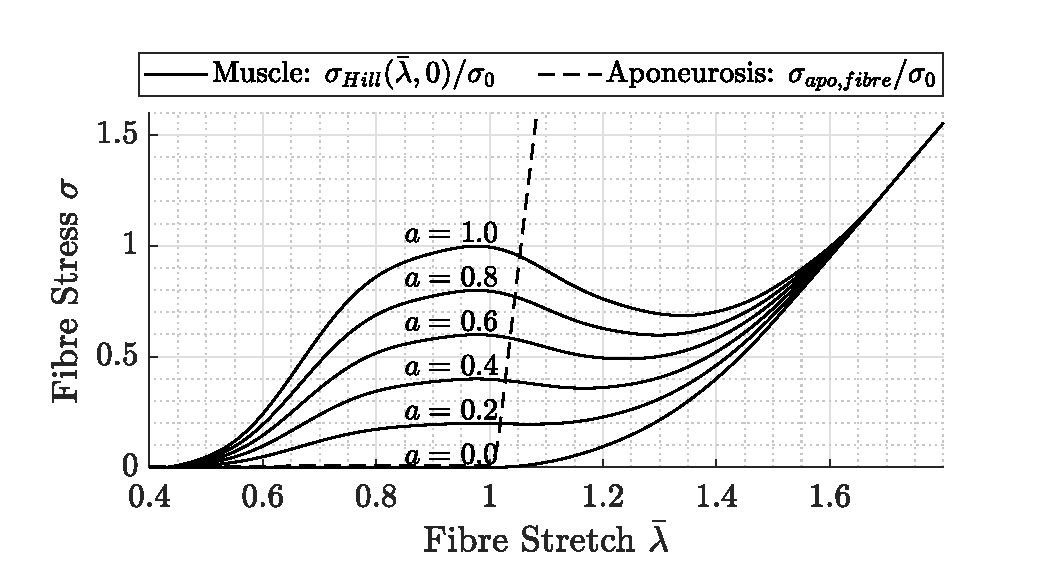
\includegraphics[width=0.49\textwidth]{fibre-FL-diff-a.eps}
    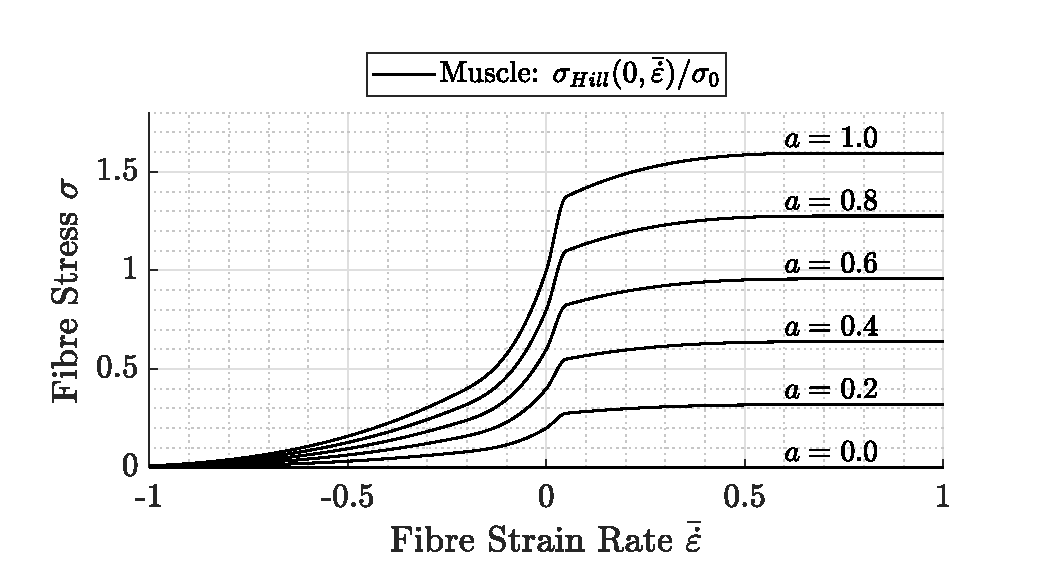
\includegraphics[width=0.49\textwidth]{fibre-FV-diff-a.eps}
    \caption{Fibre force relationships implemented in \texttt{Flexodeal} (muscle and aponeurosis) and \texttt{Flexodeal Lite} (muscle only). The code allows for continuously varying activation profiles, but for reference, we choose 6 different choices of activation level (from 0\% to 100\%) to represent the influence of the activation level on the fibre force. 
    \label{fig:FL_curves_diff_act}}
\end{figure}

We now proceed to describe the main inputs required to run \texttt{Flexodeal} and the output variables and results that the code produces. For more information on the default experiments implemented in \texttt{Flexodeal} and \texttt{Flexodeal Lite} (i.e. the experiments that users can run immediately after downloading and compiling the software), we refer the reader to Appendices \ref{app:default_flexodeal_lite} and  \ref{app:default_flexodeal}.

\subsection{Inputs}

We use distinct input files to systematically prescribe important variables, such as the boundary strain and activation profiles, as well as the marker locations used for tracking point-valued displacements.

\subsubsection{Parameter file}

Named by default \texttt{parameters.prm}, this file provides information about many scalar parameters used in the definition and finite element solution of \eqref{eq:LF_main_system}, such as:
\begin{itemize}
    \item Polynomial degree $k$ in the finite element $\*Q_{k} \times P_{k-1} \times P_{k-1}$ \eqref{eq:FE_spaces} used to approximate the solution to the three-field formulation \eqref{eq:LF_main_system}.
    \item Rule order of the Gaussian quadrature formula used to approximate integrals in the computation of local mass and stiffness matrices, as well as local forcing terms.
    \item Type of simulation: \texttt{quasi-static} or \texttt{dynamic}, per Remark \ref{re:quasi-static_dynamic}.
    \item Geometry and meshing parameters required to build the mesh.
    \item Linear solve information, such as preconditioners (\texttt{jacobi} or \texttt{ssor}) and solvers: \texttt{direct} (which uses the UMFPACK solver), \texttt{CG} (conjugate gradient), or \texttt{GMRES}.
    \item Material parameters, such as bulk moduli and the constants defining the Yeoh strain-energy functions (Table \ref{tab:constants_base_material_muscle}) for muscle, tendon, aponeurosis, and fat tissue.
    \item Nonlinear solver information, such as the maximum number of nonlinear iterations and tolerances for displacement and force\footnote{In this context, force refers to the \textit{forcing} term, i.e. the right-hand side of the linear system of equations \eqref{eq:LF_linear_system}.}, respectively denoted by $\mathtt{tol}_u$ and $\mathtt{tol}_f$. At each time step, numerical convergence of the Newton method is assessed according to the criterion:
    \[
        \vertiii{\*d \*U_k^{n+1}} \leq \mathtt{tol}_u \quad \text{and} \quad \vertiii{R(\*U_k^{n+1}, p_k^{n+1}, D_k^{n+1})} \leq \mathtt{tol}_f,
    \]
    where $\vertiii{\*d \*U_k^{n+1}}$ is the discrete $\ell^2$ norm of the vector containing the evaluation of the Newton increment for displacement $\*d \*U_k^{n+1}$ (see Section \ref{sec:newton_method}) at the degrees of freedom (in the finite element sense) of the system and $\vertiii{R(\*U_k^{n+1}, p_k^{n+1}, D_k^{n+1})}$ is the $\ell^2$ norm of the right-hand side of the linear system of equations \eqref{eq:LF_linear_system}.
    \item Time step size $\Delta t $ simulation end time $T$.
    \item Label of the boundary surface (also known as ``boundary ID'') on which the prescribed strain will be applied (see, for example, Figure \ref{fig:idealized_geometry}).
    \item Location of file containing markers (see Section \ref{sec:prescribed_act_strain}).
    \item Booleans that activate the output of binary files (see Section \ref{sec:flexodeal_outputs}).
\end{itemize}

\subsubsection{Prescribed strain and activation profiles} \label{sec:prescribed_act_strain}

Named by default \texttt{control\_points\_strain.dat} and \texttt{control\_points\_activation.dat}, these files provide respectively information about the time-dependent boundary strain $\varepsilon_M$ and activation $a$ profiles. In particular, prescribing the boundary strain implements the following boundary condition for the system of PDEs \eqref{eq:LF_main_system}:
\begin{equation}
    \*u_D = \left\{ \begin{array}{ll}
        \*0, & \text{on } \mathcal{S}_{0,\, fixed}, \\
        L_{mus} \left( \varepsilon_M(t) + 1 \right) \widehat{\bm{\ell}}, & \text{on } \mathcal{S}_{0,\, moving}.
    \end{array}\right.
\end{equation}
Here $\mathcal{S}_{0,\, fixed}, \, \mathcal{S}_{0,\, moving}  \subseteq \Gamma_{D,0}$ are respectively the fixed and moving parts of the boundary $\Gamma_{D,0}$, $L_{mus}$ is the initial length of the muscle (as defined in the parameter file), and $\widehat{\bm{\ell}}$ is the line of action vector,  which is set by default to $\langle 1,0,0 \rangle$.

In these files, information is provided as a space-separated, two-column matrix containing the pairs $(t_k, \varepsilon_M(t_k))$ (or $(t_k, a(t_k)$ for activation). The continuous profiles $\varepsilon_M(t)$ and $a(t)$ are then constructed via linear interpolation between the provided control points. As shown in Figure \ref{fig:flexodeal_lite_act_strain_profiles}, simple linear profiles can be constructed with a few control points. Since the code allows for an arbitrary number of control points, more involved profiles can be constructed as well (see Section \ref{sec:flexodeal_mri}).

\begin{figure}
    \centering
    \begin{tabular}{|>{\centering\arraybackslash}m{6cm}|}
        \hline
        \texttt{control\_points\_strain.dat} \\ \hline
        $\begin{matrix}
          0.0 & 0.0 \\
          0.1 & 0.1 \\
          0.3 & 0.1 \\
          0.5 & -0.1
        \end{matrix}$ \\
        \hline
      \end{tabular}\hspace{1em}\scalebox{1.5}{$\Rightarrow$}\hspace{1em}
      \raisebox{-5.5em}{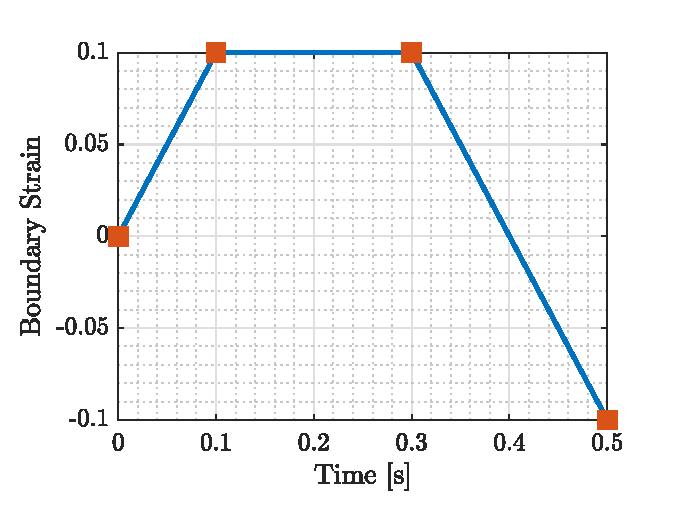
\includegraphics[width=6cm]{plot_boundary_strain.eps}}\\
      \begin{tabular}{|>{\centering\arraybackslash}m{6cm}|}
        \hline
        \texttt{control\_points\_activation.dat} \\ \hline
        $\begin{matrix}
          0.0 & 0.0 \\
          0.1 & 0.0 \\
          0.3 & 1.0 \\
          0.5 & 1.0
        \end{matrix}$ \\
        \hline
      \end{tabular}\hspace{1em}\scalebox{1.5}{$\Rightarrow$}\hspace{1em}
      \raisebox{-5.5em}{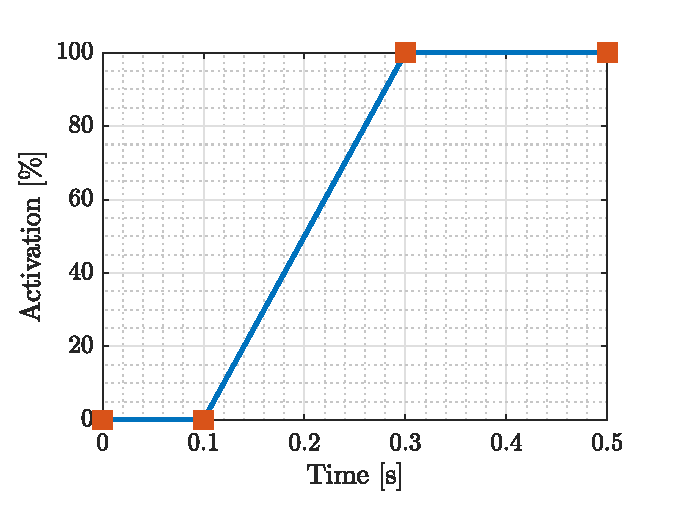
\includegraphics[width=6cm]{plot_activation.eps}}
    \caption{An example of the \texttt{.dat} files containing the necessary control points to define time-dependent curve. These particular boundary strain and activation profiles are part of the default experiment in \texttt{Flexodeal Lite} v1.5.4. \label{fig:flexodeal_lite_act_strain_profiles}}
\end{figure}

\subsubsection{Markers}

Similar to a motion capture experiment, \texttt{Flexodeal} allows the user to mark a number of mesh vertices to track their displacement. They can be provided in a space-separated text file which, by default, is named \texttt{markers.dat} and their output can be found in the CSV file \texttt{displacements-3d.csv}.

\subsubsection{Quadrature point data (not implemented in Flexodeal Lite)} 

In the context of finite element methods, many of the integrals involved in computing element stiffness matrices, mass matrices, and load vectors are not straightforward to evaluate analytically. Since exact integration may not be possible or practical for most element shapes, numerical integration is used to approximate these integrals.

%Quadrature points (QPs) are used to evaluate these integrals approximately by placing ``evaluation points'' within each element and using weights associated with these points to compute the integral. This helps in ensuring that the element-level calculations (like stiffness or mass matrices) are accurately represented in the global system, which is essential for the solution of the finite element problem.

\texttt{Flexodeal} uses a Gaussian quadrature rule. The order of this rule (which dictate the amount of QPs in each voxel) is specified in the \texttt{parameters.prm} file (see \texttt{set Quadrature order} in the \texttt{Finite element system} subsection). In Table \ref{tab:number_of_qp_points}  we provide a guideline to choose the correct quadrature rule order based on the chosen polynomial degree and whether the simulation is quasi-static or dynamic.

The QP file serves two main purposes: to list all the QPs associated to the current mesh and to attach material properties that might vary in space but not in time. Currently, the following properties are supported:
\begin{itemize}
    \item Tissue ID (column name: \texttt{tissue\_id}, SI units: none) which is set to 1 for muscle tissue, 2 for aponeurosis tissue, and 3 for tendon tissue. These IDs are set according to the material ID (also called ``physical ID'') of each cell to which a QP belongs. Therefore, the material ID of each cell may be set at the time the mesh is constructed.
    \item Muscle maximum isometric stress $\sigma_{0,mus}$ (column name: \texttt{max\_iso\_stress\_muscle}, SI units: Pa). Although this quantity (see \eqref{eq:def_hill_stress_sigma}) is usually constant throughout muscle tissue (equal to $\sim$200 kPa), some experiments might require this quantity to vary depending on fibre types \cite{Bottinelli1999}.
    \item Muscle fibre orientation (specified in three columns, \texttt{muscle\_fibre\_orientation\_x}, \texttt{muscle\_fibre\_orientation\_y}, and \texttt{muscle\_fibre\_orientation\_z}, SI units: none), a unit vector indicating orientation of a fibre passing through the QP location.
    \item Fat fraction $\chi_{fat}$ (column name: \texttt{fat\_fraction}, SI units: none), the fraction of fat (see \eqref{eq:def_kappa_bm_fat}) at the QP location.
\end{itemize}

\begin{table}
    \centering
    \begin{tabular}{|c|c|c|c|}\hline
        Polynomial degree & Type of simulation & Quadrature order & QPs per voxel \\\hline
        1 & quasi-static & 2 & 8 \\\hline
        1 & dynamic & 2 & 8 \\\hline
        2 & quasi-static & 3 & 27 \\\hline
        2 & dynamic & 4 & 64 \\\hline
        3 & quasi-static & 4 & 64 \\\hline
        3 & dynamic & 5 & 125 \\\hline
    \end{tabular}
    \caption{Minimum quadrature order required depending on the type of simulation (dynamic of quasi-static) and finite element polynomial degree.\label{tab:number_of_qp_points}}
\end{table}

\begin{remark}
    In \texttt{Flexodeal Lite}, these properties are implemented as constants throughout the domain and specified via the parameter file \texttt{parameters.prm}.
\end{remark}

\subsection{Outputs} \label{sec:flexodeal_outputs}

Several variables of physiological interest are readily available in Flexodeal.

\subsubsection{Activation and muscle length}

This CSV file (named \texttt{activation\_muscle\_length-3d.csv}) provides the time series $a(t_k)$ and $L_M(t_k)$ corresponding respectively to the activation level (in \%) and muscle length (in m) at each time step $t_k$.

\subsubsection{Displacements at predefined markers}

This CSV file (named \texttt{displacements-3d.csv}) provides 3D displacement information at the mesh vertices listed in \texttt{markers.dat}.

\subsubsection{Energies}

This CSV file (named \texttt{energy\_data-3d.csv}) provides time series for each one of the strain energies (in \unit{J \, m^{-3}}) in the system. In what follows, $|\B_t|$ denotes the volume of the current configuration $\B_t$:
\begin{itemize}
    \item Kinetic energy:
    \begin{equation}
        E_{kin}(t) = \dfrac{1}{|\B_t|} \int_{\B_0} \dfrac{1}{2} \rho_0 |\*V|^2 \ d\*X,
    \end{equation}
    \item Internal energy:
    \begin{equation}
        E_{int}(t) = \dfrac{1}{|\B_t|} \int_{\B_0} (\nabla_0 \*U) \*F^{-1} \btau \ d\*X,
    \end{equation}
    with $\btau$ as defined in \eqref{eq:def_tau},
    \item Volumetric energy:
    \begin{equation}
        E_{vol}(t) = \dfrac{1}{|\B_t|} \int_{\B_0} (\nabla_0 \*U) \*F^{-1} \btau_{vol} \ d\*X,
    \end{equation}
    with $\btau_{vol}$ as defined in \eqref{eq:def_tau_vol},
    \item Isochoric energy:
    \begin{equation}
        E_{iso}(t) = \dfrac{1}{|\B_t|} \int_{\B_0} (\nabla_0 \*U) \*F^{-1} \btau_{iso} \ d\*X,
    \end{equation}
    with $\btau_{iso}$ as defined in \eqref{eq:def_tau_iso},
    \item Muscle active energy:
    \begin{equation}
        E_{mus,act}(t) = \dfrac{1}{|\B_t|} \int_{\B_0} (\nabla_0 \*U) \*F^{-1} \btau_{mus,act} \ d\*X,
    \end{equation}
    where $\btau_{mus,act} = \p : \bar{\btau}_{mus,act}$ and $\bar{\btau}_{mus,act}$ is the active part of the $\bar{\btau}_{fibre}$ tensor defined in \eqref{eq:def_tau_bar_fibre}, that is:
    \[
        \bar{\btau}_{mus,act} = \dfrac{1}{\bar{\lambda}^2} \sigma_{0,mus}  a(\*X,t) \widehat{\sigma}_A(\bar{\lambda}) \widehat{\sigma}_V(\bar{\depsilon})  \bar{\*a} \otimes \bar{\*a},
    \]
    \item Muscle passive energy:
    \begin{equation}
        E_{mus,pas}(t) = \dfrac{1}{|\B_t|} \int_{\B_0} (\nabla_0 \*U) \*F^{-1} \btau_{mus,pas} \ d\*X,
    \end{equation}
    analogous to the muscle active energy,  $\btau_{mus,pas} = \p : \bar{\btau}_{mus,pas}$ and:
    \[
        \bar{\btau}_{mus,pas} = \dfrac{1}{\bar{\lambda}^2} \sigma_{0,mus}  \widehat{\sigma}_P(\bar{\lambda})  \bar{\*a} \otimes \bar{\*a},
    \]
    \item Aponeurosis fibre energy:
    \begin{equation}
        E_{apo,fibre}(t) = \dfrac{1}{|\B_t|} \int_{\B_0} (\nabla_0 \*U) \*F^{-1} \btau_{apo,fibre} \ d\*X,
    \end{equation}
    with $\btau_{apo,fibre} = \p : \bar{\btau}_{apo,fibre}$ and $\bar{\btau}_{apo,fibre}$ as defined in \eqref{eq:def_tau_bar_tis_fibre},
    \item Aponeurosis base material energy:
    \begin{equation}
        E_{apo,bm}(t) = \dfrac{1}{|\B_t|} \int_{\B_0} (\nabla_0 \*U) \*F^{-1} \btau_{apo,bm} \ d\*X,
    \end{equation}
    with $\btau_{apo,bm} = \p : \bar{\btau}_{apo,bm}$ and $\bar{\btau}_{apo,bm}$ as defined in \eqref{eq:def_tau_bar_tis_bm},
    \item Tendon fibre energy:
    \begin{equation}
        E_{ten,fibre}(t) = \dfrac{1}{|\B_t|} \int_{\B_0} (\nabla_0 \*U) \*F^{-1} \btau_{ten,fibre} \ d\*X,
    \end{equation}
    with $\btau_{ten,fibre} = \p : \bar{\btau}_{ten,fibre}$ and $\bar{\btau}_{ten,fibre}$ as defined in \eqref{eq:def_tau_bar_tis_fibre},
    \item Tendon base material energy:
    \begin{equation}
        E_{ten,bm}(t) = \dfrac{1}{|\B_t|} \int_{\B_0} (\nabla_0 \*U) \*F^{-1} \btau_{ten,bm} \ d\*X,
    \end{equation}
    with $\btau_{ten,bm} = \p : \bar{\btau}_{ten,bm}$ and $\bar{\btau}_{ten,bm}$ as defined in \eqref{eq:def_tau_bar_tis_bm}.
\end{itemize}

Therefore, the computed energies satisfy the additive relationships:
\begin{equation}
    E_{int} = E_{vol} + E_{iso},
\end{equation}
and
\begin{equation}
    E_{iso} = E_{mus,act} + E_{mus,pas} + E_{apo,fibre} + E_{apo,bm} + E_{ten,fibre} + E_{ten,bm}.
\end{equation}

\subsubsection{Forces}

Muscle forces are essential because they represent the active mechanical output generated by muscle fibres and transmitted to the tendon, ultimately enabling joint motion and force application to the skeleton. Therefore, it is of great physiological interest to compute these forces at particular surfaces of the muscle-tendon unit.

The general expression for the force exerted on a surface $\mathcal{S}_t \subseteq \partial \B_t$ of the body whose current configuration is $\B_t$ is given by:
\begin{equation} \label{eq:def_force_general}
    \vec{F}(t) = \int_{\mathcal{S}_t} \bsigma \*n \ ds = \int_{\mathcal{S}_0} J \bsigma \*F^{-\top} \*N \ dS = \int_{\mathcal{S}_0} \btau \*F^{-\top} \*N \ dS.
\end{equation}
Here, we have used Nanson's formula \eqref{eq:differentials}\textsubscript{2} to transform the surface from its current configuration $\mathcal{S}_t$ to the reference configuration $\mathcal{S}_0$. However, $\btau$ is a quantity that is only available at \textit{interior} quadrature points, so the expression in \eqref{eq:def_force_general} can only be \textit{estimated}. In particular, the force at a surface $\mathcal{S}_0$ is approximated in \texttt{Flexodeal} using the last equality in \eqref{eq:def_force_general}:
\begin{equation} \label{eq:def_force_approximated}
    \vec{F}(t) \approx \sum_{T \in \mathcal{T}_h(\mathcal{S}_0)} \ \sum_{q = 1}^{N_q^\partial} \btau(\widetilde{\*X}_q, t) \, \*F^{-\top}(\widetilde{\*X}_q, t) \, \*N(\*X_q, t) \, J_{T \to \Box} \, w_q,
\end{equation}
where $\mathcal{T}_h(\mathcal{S}_0)$ is a tesselation (made of quadrilaterals) of the surface $\mathcal{S}_0$, $(\*X_q, w_q)_{q = 1}^{N_q^\partial}$ is a Gaussian quadrature on the unit square $\Box$ (of the same order as the one used in computing the volume integrals) with points $\*X_q$ and weights $w_q$, $J_{T \to \Box}$ is the Jacobian of the affine transformation that maps $T$ into $\Box$, and $\widetilde{\*X}_q$ is the closest interior quadrature point to the surface quadrature point $\*X_q$.

These forces are written to disk in the files:
\begin{center}
    \texttt{force\_data-3d-XYZ.csv} and \texttt{force\_data-3d.csv}.
\end{center}
The first file exports the force derived from the different Kirchhoff stresses that are computed in the code (e.g. $\btau$, $\btau_{vol}$, $\btau_{iso}$, etc.) at each part of the boundary $\partial \B_0$, where XYZ is a suffix used to identify a particular time step. The second file exports the $x$ component of the force vector $\vec{F}$ at the boundary ID indicated in the parameter ``\texttt{set Pulling face ID}'' of the parameter file, since this is typically a quantity of interest in lengthening/shortening experiments. 

The force $\vec{F}$ computed in \eqref{eq:def_force_general} corresponds to the total force arising from all the material components of the system, that is, using the stress tensor $\btau$. To compute individual contributions to this force, we modify the Kirchhoff stress to be used in \eqref{eq:def_force_general} and proceed as in the computation of energies. This leads to the following quantities, which are available in all force-related CSV files:
\begin{itemize}
    \item Volumetric force $\vec{F}_{vol}$ computed using $\btau_{vol}$,
    \item Isochoric force $\vec{F}_{iso}$ computed using $\btau_{iso}$,
    \item Muscle active force $\vec{F}_{mus,act}$ computed using $\btau_{mus,act}$,
    \item Muscle passive force $\vec{F}_{mus,pas}$ computed using $\btau_{mus,pas}$,
    \item Muscle base material $\vec{F}_{mus,bm}$ computed using $\btau_{mus,bm}$,
    \item Aponeurosis fibre force $\vec{F}_{apo,fibre}$ computed using $\btau_{apo,fibre}$,
    \item Aponeurosis base material $\vec{F}_{apo,bm}$ computed using $\btau_{bm,fibre}$,
    \item Tendon fibre force $\vec{F}_{ten,fibre}$ computed using $\btau_{ten,fibre}$,
    \item Tendon base material force $\vec{F}_{ten,bm}$ computed using $\btau_{ten,apo}$.
\end{itemize}
Therefore, the following additive relationships hold:
\begin{equation}
    \vec{F} = \vec{F}_{vol} + \vec{F}_{iso},
\end{equation}
and
\begin{equation}
    \vec{F}_{iso} = \vec{F}_{mus,act} + \vec{F}_{mus,pas} + \vec{F}_{mus,bm} + \vec{F}_{apo,fibre} + \vec{F}_{apo,bm} + \vec{F}_{ten,fibre} + \vec{F}_{ten,bm}.
\end{equation}

\subsubsection{Gearing-related information} \label{sec:flexodeal-gearing-related-info}

Gearing refers to the relationship between the muscle's overall shortening (or lengthening) speed and the shortening (or lengthening) speed of its individual muscle fibres \cite{Azizi2008VariableGearing,Eng2018}. This is a concept that we discuss in detail in Chapter \ref{ch:gearing}. This file, named \texttt{gearing\_info-3d.csv}, contains the following information:
\begin{itemize}
    \item $x$-component of the prescribed velocity at the moving end of the muscle, computed using the prescribed boundary strain $\varepsilon_M$ (see Section \ref{sec:prescribed_act_strain}) at each time step $t_k$ as
    \begin{equation}
        V_M(t_k) = L_{mus} \dfrac{\varepsilon_M(t_k) - \varepsilon_M(t_{k-1})}{\Delta t},
    \end{equation}
    \item Mean muscle velocity, computed as:
    \begin{equation}
        \mathrm{avg}_\mathrm{S}(\*V_{mus})(t) = \dfrac{1}{|\mathrm{slab}(\B_t)|} \int_{\mathrm{slab}(\B_0)} \*V(\*X,t) J(\*X,t) \ d\*X,
    \end{equation}
    where
    \begin{equation}
        \mathrm{slab}(\B_0) := \left\{ \*X = (x_1,x_2,x_3) \in \B_0 : \dfrac{3}{8}L_{mus} \leq x_1 \leq \dfrac{5}{8} L_{mus} \right\}
    \end{equation}
    is a subregion of the reference configuration $\B_0$ that removes the ends of the domain (assuming its length runs along the $x$ direction) to leave out of consideration nonphysical effects that may happen at the Dirichlet boundaries. Naturally, we have $\mathrm{slab}(\B_t) = \bm{\varphi} \left(\mathrm{slab}(\B_0), t \right)$ where $\bm{\varphi}$ is the deformation that maps $\B_0$ into $\B_t$.
    \item Mean fibre strain rate, computed as:
    \begin{equation} \label{eq:def_mean_fibre_strain_rate}
        \mathrm{avg}_\mathrm{S}(\dot{\varepsilon})(t) = \dfrac{1}{|\mathrm{slab}(\B_t)|} \int_{\mathrm{slab}(\B_0)} \dot{\varepsilon}(\*X,t) J(\*X,t) \ d\*X,
    \end{equation}
    where $\dot{\varepsilon}$ is the fibre strain rate defined in \eqref{eq:def_strain_rate_fibre_non_bar}. 
\end{itemize}

\subsubsection{Mean fibre stretch and pennation}

These time series are located in the \texttt{mean\_stretch\_pennation\_data.csv} file. First, similar to the mean fibre strain rate in \eqref{eq:def_mean_fibre_strain_rate}, the mean fibre stretch is computed on the region $\mathrm{slab}(\B_t)$ at each time $t \geq 0$ according to \eqref{eq:def_lambda_bar}, that is
\begin{equation} \label{eq:def_mean_fibre_stretch}
    \mathrm{avg}_\mathrm{S}(\lambda)(t) = \dfrac{1}{|\mathrm{slab}(\B_t)|} \int_{\mathrm{slab}(\B_0)} \lambda(\*X,t) J(\*X,t) \ d\*X.
\end{equation}

We define the pennation $\beta(\*X,t)$ of a muscle fibre passing through $\*X$  in the sense of Lieber \& Frid\'{e}n \cite{LieberFriden2000}, that is, as the angle between its current orientation $\*F \*a_0$ and the muscle's axis of force generation, which we assume to coincide with the line of action vector $\widehat{\bm{\ell}}$. Therefore,
\begin{equation}
    \beta(\*X,t) = \cos^{-1} \left( \dfrac{\*a(\*X,t) \cdot \widehat{\bm{\ell}}}{\lambda(\*X,t)} \right), \quad \*a(\*X,t) := \*F(\*X,t) \*a_0(\*X).
\end{equation}
Furthermore, since we are assuming that $\widehat{\bm{\ell}} = \langle 1,0,0 \rangle$, we have that the pennation can be computed from the first component of the current orientation vector $\*a = \langle a_1,a_2,a_3 \rangle$, that is:
\begin{equation}
    \beta(\*X,t) = \cos^{-1} \left( \dfrac{a_1}{\lambda} \right).
\end{equation}

The initial pennation angle is denoted by $\beta_0(\*X) = \beta(\*X,0)$. For $t>0$, the mean pennation angle over the region $\mathrm{slab}(\B_t)$ is therefore given by:
\begin{equation} \label{eq:def_mean_fibre_pennation}
    \mathrm{avg}_\mathrm{S}(\beta)(t) = \dfrac{1}{|\mathrm{slab}(\B_t)|} \int_{\mathrm{slab}(\B_0)} \beta(\*X,t) J(\*X,t) \ d\*X.
\end{equation}

\subsubsection{Mechanical variables at all QPs (binary files)} \label{sec:binary_files}

These set of files, named 
\begin{center}
    \texttt{cell\_data\_main-3d-XYZ.data} and \texttt{cell\_data\_tensors-3d-XYZ.data}    
\end{center}
provide detailed QP information about most of the variables computed in Flexodeal, where XYZ is a suffix used to identify a particular time step. Each file contains an 2D array with a fixed number of columns and a fixed number of rows, the latter corresponding to the total number of quadrature points in the system. A description of the columns in each one of these files can be found respectively in Tables \ref{tab:contents_binary_file_main} and \ref{tab:contents_binary_file_tensors}.

\begin{table}
    \centering
    \begin{tabular}{|>{\centering\arraybackslash}m{1.3cm}|>{\centering\arraybackslash}m{3.2cm}|>{\centering\arraybackslash}m{8cm}|}
        \hline
        Column & Variable & Description \\\hline
        1 & \texttt{qp\_x} & X component of the QP in the reference configuration [m] \\\hline
        2 & \texttt{qp\_y} & Y component of the QP in the reference configuration [m]\\\hline
        3 & \texttt{qp\_z} & Z component of the QP in the reference configuration [m]\\\hline
        4 & \texttt{JxW} & Dilatation multiplied by the quadrature rule weight at this point \\\hline
        5 & \texttt{det\_F} & Determinant of the deformation tensor $\*F$ \\\hline
        6 & \texttt{u1} & First displacement component [m]\\\hline
        7 & \texttt{u2} & Second displacement component [m] \\\hline
        8 & \texttt{u3} & Third displacement component [m] \\\hline
        9 & \texttt{v1} & First velocity component [\unit{m \, s^{-1}}]\\\hline
        10 & \texttt{v2} & Second velocity component [\unit{m \, s^{-1}}] \\\hline
        11 & \texttt{v3} & Third velocity component [\unit{m \, s^{-1}}] \\\hline
        12 & \texttt{p} & Pressure $p$ [Pa] \\\hline
        13 & \texttt{D} & Dilatation $D$ [nondim]\\\hline
        14 & \texttt{stretch} & Fibre stretch $\lambda$ [nondim] \\\hline
        15 & \texttt{stretch\_bar} & Modified fibre stretch $\bar{\lambda}$ [nondim] \\\hline
        16 & \texttt{strain\_rate} & Fibre strain rate $\depsilon$ [nondim] \\\hline
        17 & \texttt{strain\_rate\_bar} & Modified fibre strain rate $\bar{\depsilon}$ [nondim] \\\hline
        18 & \texttt{orientation\_x} & X component of current fibre orientation \\\hline
        19 & \texttt{orientation\_y} & Y component of current fibre orientation \\\hline
        20 & \texttt{orientation\_z} & Z component of current fibre orientation \\\hline
        21 & \texttt{tissue\_id} & Tissue ID \\\hline
      \end{tabular}
      \caption{Contents of the file \texttt{cell\_data\_main-3d-XYZ.data}.\label{tab:contents_binary_file_main}}
\end{table}

\begin{table}
    \centering
    \begin{tabular}{|>{\centering\arraybackslash}m{1.3cm}|>{\centering\arraybackslash}m{4.8cm}|>{\centering\arraybackslash}m{8cm}|}
        \hline
        Column & Variable & Description \\\hline
        1 & \texttt{qp\_x} & X component of the QP in the reference configuration [m] \\\hline
        2 & \texttt{qp\_y} & Y component of the QP in the reference configuration [m]\\\hline
        3 & \texttt{qp\_z} & Z component of the QP in the reference configuration [m]\\\hline
        4 & \texttt{JxW} & Dilatation multiplied by the quadrature rule weight at this point \\\hline
        5 & \texttt{det\_F} & Determinant of the deformation tensor $\*F$ \\\hline
        6-14 & \texttt{F\_i\_j} & Components of the deformation tensor $\*F$ \\\hline
        15-23 & \texttt{tau\_i\_j} & Components of the Kirchhoff stress $\btau$ \\\hline
        24-32 & \texttt{tau\_vol\_i\_j} & Components of the Kirchhoff stress $\btau_{vol}$ \\\hline
        33-41 & \texttt{tau\_iso\_i\_j} & Components of the Kirchhoff stress $\btau_{iso}$ \\\hline
        42-50 & \texttt{tau\_muscle\_active\_i\_j} & Components of the Kirchhoff stress $\btau_{mus,act}$ \\\hline
        51-59 & \texttt{tau\_muscle\_passive\_i\_j} & Components of the Kirchhoff stress $\btau_{mus,pas}$ \\\hline
        60-68 & \texttt{tau\_muscle\_base\_i\_j} & Components of the Kirchhoff stress $\btau_{bm}$ \\\hline
        69 & \texttt{tissue\_id} & Tissue ID \\\hline
    \end{tabular}
    \caption{Contents of the file \texttt{cell\_data\_tensors-3d-XYZ.data}. Each tensor is stored in row order, that is, the 9 columns contain information of the (1,1), (1,2), (1,3), (2,1), \dots, (3,2), and (3,3) components.
    \label{tab:contents_binary_file_tensors}}
\end{table}

\subsubsection{VTU files}

To visualize the solutions in 3D space, we export several VTU files that can be opened in software such as Paraview or Visio. The main variables (displacement, pressure, and dilatation) are exported at each time step (denoted by the suffix \texttt{XYZ}) in the \texttt{solution-3d-XYZ.vtu}. These are constructed directly from the DOFs of the finite element solution. In turn, variables that are stored only at quadrature points, such as stresses, fibre stretches, and fibre strain rates, are first projected onto an appropriate finite element space and then exported to VTU format. In particular, at each time step \texttt{XYZ}, the following files are available:
\begin{itemize}
    \item \texttt{strain\_rate-3d-XYZ.vtu} which contains the fibre strain rate field $\depsilon(\*X,\cdot)$ computed via projection onto the \texttt{FE\_DGQ} finite element of order $k$ (same order as in the displacement finite element). This is a discontinuous element similar to $P_k$ (see \eqref{eq:Hhp}) but based on Lagrange polynomials rather than monomials.
    \item \texttt{stress-3d-XYZ.vtu} which contains each of the 9 components\footnote{Technically, only 6 components are required since this is a symmmetric tensor.} of the Kirchhoff stress $\btau$, computed via projection onto the \texttt{FE\_DGQ} finite element of order $k-1$.
    \item \texttt{stretch-3d-XYZ.vtu} which contains the fibre stretch $\lambda(\*X,\cdot)$ as well as the three components of the current orientation vector $\*a = \*F \*a_0$, both of them projected component-wise onto \texttt{FE\_DGQ} elements. In Paraview, this file can also be used to visualize bundles of individual fibres as streamlines of the vector field $\*a(\*X,t)$, as we do for instance in Figure \ref{fig:convergence_space_3d_plots}.
    \item \texttt{velocity-3d-XYZ.vtu} which contains the velocity field $\*V(\*X,\cdot)$, computed via projection from the stored quadrature-point information onto $\*Q_k$ elements (see \eqref{eq:Hhu}).
\end{itemize}

\subsubsection{Other outputs}

For reference, we also export the grid that was used in each experiment as \texttt{grid-3d.msh} and the parameters file as \texttt{parameters.prm}.


\section{Convergence studies} \label{sec:flexodeal_convergence}

In this section, we study the convergence of the finite element (FE) approximation of the nonlinear weak formulation \eqref{eq:LF_weak} using the spaces described in \eqref{eq:FE_spaces}. In general, we will consider sufficiently refined solutions as ``exact'' solutions for the error computation. To compare solutions computed using different meshes, we develop a separate code in which we reconstruct the solutions from their QP data using suitable projections. This helps preserve the structure of the core components of Flexodeal. We explain our choices next, before diving into the particulars of the convergence study.

\subsection{Error computation}

Let $(\*U_{h_f}, p_{h_f}, D_{h_f})$ and $\left(\*U_{h_c}, p_{h_c}, D_{h_c}\right)$ be finite element (FE) solutions to the problem \eqref{eq:LF_main_system} using discretizations $\mathcal{T}_{h_f}$ and $\mathcal{T}_{h_c}$, respectively. We assume that the mesh $\mathcal{T}_{h_f}$ is finer than $\mathcal{T}_{h_c}$, so we may refer to them (and their associated FE solutions) as the ``fine'' and ``coarse'' meshes. We are interested in computing
\[
  \| \*U_{h_f} - \*U_{h_c} \|_{\*L^2(\B_0)}, \quad \| p_{h_f} - p_{h_c} \|_{L^2(\B_0)}, \quad \text{and} \quad  \| D_{h_f} - D_{h_c} \|_{L^2(\B_0)},
\]
at some time $t > 0$. Using the pressure field as an example, we notice that
\begin{align}
    \| p_{h_f} - p_{h_c} \|_{L^2(\B_0)}^2 &= \displaystyle \sum_{T \in \mathcal{T}_{h_c}} \int_{T} (p_{h_f}(\*X, t) - p_{h_c}(\*X, t))^2 \ d\*X \notag \\
    &= \displaystyle \sum_{T \in \mathcal{T}_{h_c}} \int_{\Box} (p_{h_f}(\*X, t) - p_{h_c}(\*X, t))^2 J_{T \to \Box} \ d\*X \notag \\
    &\approx \displaystyle \sum_{T \in \mathcal{T}_{h_c}} \sum_{q=1}^{N_q^c} (p_{h_f}(\*X_q, t) - p_{h_c}(\*X_q, t))^2 J_{T \to \Box} \ w_q, \label{eq:error_p_discrete}
\end{align}
where $(\*X_q, w_q)$ are the QPs and weights of the quadrature rule associated to the coarse mesh. Therefore, while the quantities $p_{h_c}(\*X_q,t)$ and $J_{T \to \Box}$, and $w_q$ are available in the binary files that \texttt{Flexodeal} exports (see Section \ref{sec:binary_files}), we must find a way to compute $p_{h_f}(\*X_q,t)$, i.e. the \textit{fine} solution at the QPs of the \textit{coarse} mesh. This is performed in four steps:
\begin{enumerate}
    \item Read the binary file corresponding to the fine solution and store the data in an appropriate structure,
    \item Project the data into an evaluable FE solution, that is, solve the problem: find $\widetilde{p_h} \in L^2(\B_0)$ such that
    \[
    \int_{\B_0} \widetilde{p_h} q  \ d\*X = \int_{\B_0} p_{h_f} q_h \ d\*X, \quad \forall \ q_h \in L^2(\B_0),
    \]
    which is a solvable problem since we have the necessary QP information for $p_{h_f}$ in the fine solution,
    \item Evaluate $\widetilde{p_h}$ at the QPs of the coarse mesh (using the \texttt{VectorTools::point\_difference} function from deal.II),
    \item Export the results to a CSV file and compute \eqref{eq:error_p_discrete} externally.
\end{enumerate}
In this way, solutions corresponding to different refinements can be computed independent of each other, allowing the user to perform convergence studies \textit{without} modifying the core code of Flexodeal.

\subsection{Isometric contractions}

In what follows, we will consider the following definition of an isometric contraction.

\begin{definition}[Isometric contraction in the Flexodeal framework] \label{def:isometric_contraction_3d}
    Consider a muscle-tendon unit (MTU) whose current configuration occupies a region $\B_t \subset \R^3$. Furthermore, assume this region has a boundary $\partial\B_t = \Gamma_D \cup \Gamma_N$, where $\Gamma_D \cap \Gamma_N = \emptyset$, and $\Gamma_D,\Gamma_N$ represent respectively the Dirichlet and Neumann boundaries of the domain. We say that a contraction is \textit{isometric} if the MTU is activated from 0\% to a pre-defined maximum activation level $a_{max}$ over a timespan of $T$ seconds, subject to the following boundary conditions:
    \[
        \*u = \*0 \quad \text{on }\Gamma_D, \qquad \bsigma\*n = \*0 \quad \text{on } \Gamma_N,
    \]
    with equivalent Lagrangian boundary conditions when the contraction starts from its initial configuration $\B_0$.
\end{definition}

Therefore, when $\Gamma_D$ coincides with the ends of the muscle (as it is our case here), an isometric contraction maintains the (current) length of the MTU constant while allowing the fibres to deform. In this setup, isometric contractions are yet another example of a dynamic contraction for which force-velocity properties are perfectly applicable. After all, strains are nonuniform throughout the muscular structure \cite{BlemkerDelp2005}, so velocity changes are expected to happen within. We will discuss these effects in more detail in Section \ref{sec:flexodeal_dynamic_effects}.

\subsection{Setup}

\begin{figure}
    \centering
    \includegraphics[width=0.9\textwidth]{geometry_muscle_block_with_pennation.pdf}
    \caption{Muscle block geometry, including a 3D view (top) and the main quantities that describe the muscle architecture (bottom). In particular, the fibres are parallel to each other and oriented with an initial pennation angle $\beta_0$ in the $xz$ plane, which results in an initial orientation field $\*a_0(\*X) = \langle \cos(\beta_0), 0, \sin(\beta_0) \rangle$ for any $\*X \in \B_0$.\label{fig:muscle_block}}
\end{figure}

We considered the domain and muscle architecture described in Figure \ref{fig:muscle_block}, which we henceforth refer to as the ``muscle block''. We also assumed that the block had dimensions $L_{mus} = 3 \ \unit{cm}$, $W_{mus} = H_{mus} = 1 \ \unit{cm}$ and an initial pennation angle of $\beta_0 = 30^\circ$. Assuming a constant density of $\rho_0 = 1,060 \ \unit{kg \ m^{-3}}$, the block therefore had a mass of 3.18 \unit{g}. 

We discretized the muscle block by subdividing its length, width, and height into $2^n$ segments, where $n \in \mathbb{N}$ is called \textit{grid refinement level} (GRL), which resulted in a mesh with $2^{3n}$ voxels and $125 \times 2^{3n}$ quadrature points (a quadrature rule of order 5 was used). In this case, the mesh size is given by the diameter of each voxel, that is
\[
    h = 2^{-n} \sqrt{L_{mus}^2 + W_{mus}^2 + H_{mus}^2} = 2^{-n} \sqrt{11} \ \unit{cm}.
\]
Therefore, to simplify the presentation, we refer to each mesh according to its GRL rather than to its mesh size $h$.

We performed an isometric contraction where the activation was linearly ramped up from 0\% at $t=0 \ \unit{s}$ to 100\% at $t = T := 0.2 \ \unit{s}$ (i.e., over 200 ms). In particular, the fixed ends correspond to the +x and -x faces of the block. The other faces were traction free.

To study the convergence in time of the (nonlinear) finite element method, we compute the relative errors:
\begin{subequations}
    \begin{eqnarray}
        e^{\*U}_{\Delta t} &:= \dfrac{\norm{\*U_{\Delta t}(\cdot,T) - \*U(\cdot,T)}_{\*L^2(\B_0)}}{\norm{\*U(\cdot,T)}_{\*L^2(\B_0)}}, \\
        e^p_{\Delta t} &:= \dfrac{\norm{p_{\Delta t}(\cdot,T) - p(\cdot,T)}_{L^2(\B_0)}}{\norm{p(\cdot,T)}_{L^2(\B_0)}}, \\
        e^D_{\Delta t} &:= \dfrac{\norm{D_{\Delta t}(\cdot,T) - D(\cdot,T)}_{L^2(\B_0)}}{\norm{D(\cdot,T)}_{L^2(\B_0)}},
    \end{eqnarray}
\end{subequations}
for a fixed GRL = 3 and time step sizes $\Delta t = 1/(10 \cdot 2^{k+1}) \ \unit{s}$, $k = 1, \dots, 5$. We compare these approximations $(\*U_{\Delta t}, p_{\Delta t}, D_{\Delta t})$ with a more refined solution $(\*U, p, D)$ computed with $\Delta t = 1/(10 \cdot 2^8) \ \unit{s}$. For two different time step sizes $\Delta t$, $\Delta t'$, with $\Delta t > \Delta t'$, we also compute the rate of convergence as
\begin{equation}
    r^{\star}_t := \dfrac{\log \left(e^\star_{\Delta t} / e^\star_{\Delta t'} \right)}{\log \left(\Delta t / \Delta t'  \right)}, \quad \star \in \{ \*U, p, D \}.
\end{equation}

To study the convergence in space, we compute the relative errors:
\begin{subequations}
    \begin{eqnarray}
        e^{\*U}_{h} &:= \dfrac{\norm{\*U_{h}(\cdot,T) - \*U(\cdot,T)}_{\*L^2(\B_0)}}{\norm{\*U(\cdot,T)}_{\*L^2(\B_0)}}, \\
        e^p_{h} &:= \dfrac{\norm{p_{h}(\cdot,T) - p(\cdot,T)}_{L^2(\B_0)}}{\norm{p(\cdot,T)}_{L^2(\B_0)}}, \\
        e^D_{h} &:= \dfrac{\norm{D_{h}(\cdot,T) - D(\cdot,T)}_{L^2(\B_0)}}{\norm{D(\cdot,T)}_{L^2(\B_0)}},
    \end{eqnarray}
\end{subequations}
for a fixed time step size $\Delta t = 0.01 \ \unit{s}$ and GRL = 2, 3, 4, and 5. The approximations $(\*U_h, p_h, D_h)$ are compared to a refined solution $(\*U,p,D)$ computed using a GRL = 6. For two different mesh sizes $h,h'$ (coming in particular from different GRLs), with $h>h'$, we compute the associated rates of convergence:
\begin{equation}
    r^\star_\*x := \dfrac{\log \left(e^\star_{h} / e^\star_{h'} \right)}{\log \left(h / h'  \right)}, \quad \star \in \{ \*U, p, D \}.
\end{equation}
The solutions were computed using \texttt{Flexodeal Lite} v1.5.1 and a $Q_2/P_1$ element. The linear systems were solved using a CG solver with a Jacobi preconditioner. Furthermore, the force and displacement tolerances for the nonlinear solver were set to $10^{-4}$. We set the quadrature order to 5, which was above the required number of quadrature points according to Table \ref{tab:number_of_qp_points} to capture forces more accurately. This will be a constant choice throughout this thesis.

\subsection{Main results}

In Figure \ref{fig:convergence_space_3d_plots} we show the experiment performed for this convergence study according to the setup previously described. Furthermore, in Figure \ref{fig:convergence_dynamic}, we portray the corresponding error curves for the study of the dynamic problem. First, we observe from Figure \ref{fig:convergence_dynamic} (left) that the numerical method converges with rate $\mathcal{O}(\Delta t)$ (see also Table \ref{tab:errors_rates_time}), which matches the fact that velocities and accelerations have been discretized using first-order difference formulas. Next, from Figure \ref{fig:convergence_dynamic} (right), we observe that in the space variables, the displacement converges with rate $\mathcal{O}(h)$ (in the $\*L^2(\B_0)$ norm), whereas the pressure and dilation converge with rate $\mathcal{O}(h^{3/2})$ (see also Table \ref{tab:errors_rates_space}). These rates are certainly much lower than the $\mathcal{O}(h^3)$ and $\mathcal{O}(h^2)$ expected respectively for the linear iterations (see \eqref{eq:a_priori_linear_problem}). Multiple reasons contribute to this phenomenon. As mentioned in Section \ref{sec:FE_approximation_properties}, the latter are rates that can only be expected for a single Newton iteration and only if the increments are sufficiently smooth (the fact that the muscle architecture is pennate and that the muscle is activated to 100\% likely contribute to the lack of smoothness). However, this should not be understood as a failure of the implemented numerical method, but rather as a first (and honest) sign of the true complexity of three-dimensional, dynamic, fully active musculoskeletal simulation. 

\begin{figure}
    \centering
    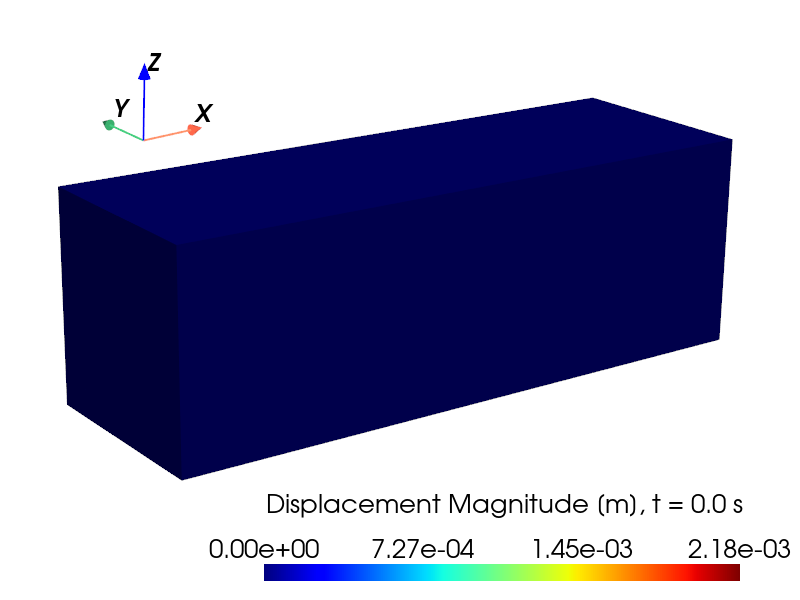
\includegraphics[width=0.45\textwidth]{convergence-space-disp-000.png}\hspace{2em}
    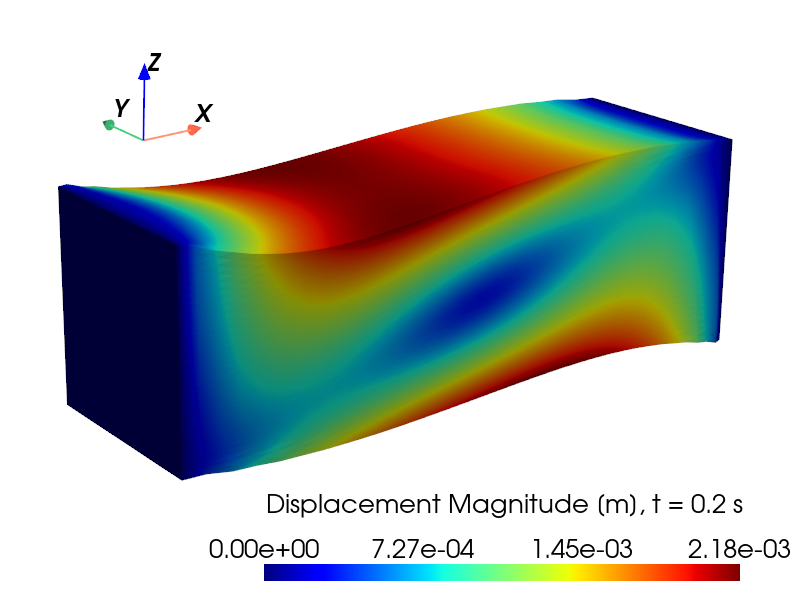
\includegraphics[width=0.45\textwidth]{convergence-space-disp-020.png}\\
    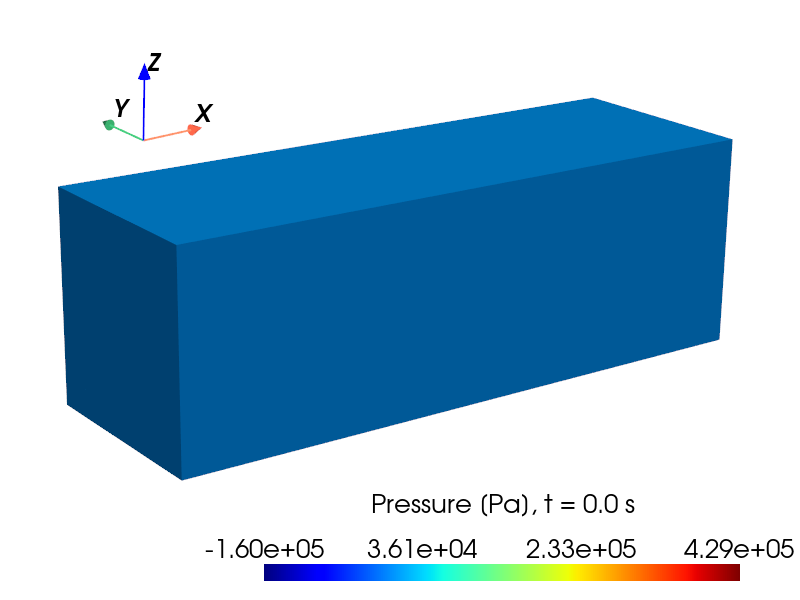
\includegraphics[width=0.45\textwidth]{convergence-space-pre-000.png}\hspace{2em}
    \includegraphics[width=0.45\textwidth]{convergence-space-pre-020.png}\\
    \includegraphics[width=0.45\textwidth]{convergence-space-dil-000.png}\hspace{2em}
    \includegraphics[width=0.45\textwidth]{convergence-space-dil-020.png}\\
    \includegraphics[width=0.45\textwidth]{convergence-space-lam-000.png}\hspace{2em}
    \includegraphics[width=0.45\textwidth]{convergence-space-lam-020.png}
    \caption{Visualization of the displacement $\*U$, pressure $p$, dilatation $D$, and fibre stretch $\lambda$ fields for the convergence study described in Section \ref{sec:flexodeal_convergence}. Left column: initial state ($t=0.0$ s) showing $(\*U,p,D) = (\*0,0,1)$ and $\lambda = 1$. Right column: end state ($t = 0.2$ s).
    \label{fig:convergence_space_3d_plots}}
\end{figure}

\begin{figure}
    \centering
    \includegraphics[width=0.48\textwidth]{convergence-study-time.eps}
    \includegraphics[width=0.48\textwidth]{convergence-study-space.eps}
    \caption{Relative $L^2$ error in the displacement, pressure, and dilatation variables, measured at the end of the simulation time, using a dynamic computation. Left: error as $\Delta t$ decreases while the grid refinement level is fixed to 3. Right: error as the grid refinement level increases while keeping $\Delta t = 0.01 \unit{s}$.\label{fig:convergence_dynamic}}
\end{figure}

\begin{table}
\centering
\small
\begin{tabular}{ccccccc}
\hline
$\Delta t$ [ms] &  $e_{\Delta t}^{\*U}$ & $r_{t}^\*U$ & $e_{\Delta t}^{p}$ & $r_{t}^p$  & $e_{\Delta t}^{D}$ & $r_{t}^D$  \\
\hline
25.0000  & $8.5965 \times 10^{-3}$ & -       & $1.6034 \times 10^{-2}$ & -       & $6.7261 \times 10^{-5}$ & - \\
12.5000  & $4.2794 \times 10^{-3}$ & 1.0064  & $8.0023 \times 10^{-3}$ & 1.0026  & $3.3572 \times 10^{-5}$ & 1.0025 \\
6.2500   & $2.0821 \times 10^{-3}$ & 1.0393  & $3.8993 \times 10^{-3}$ & 1.0372  & $1.6359 \times 10^{-5}$ & 1.0371 \\
3.1250   & $9.7413 \times 10^{-4}$ & 1.0959  & $1.8258 \times 10^{-3}$ & 1.0947  & $7.6606 \times 10^{-6}$ & 1.0946 \\
1.5625   & $4.1786 \times 10^{-4}$ & 1.2211  & $7.8361 \times 10^{-4}$ & 1.2203  & $3.2883 \times 10^{-6}$ & 1.2201 \\
\hline
\end{tabular}
\caption{Errors and convergence rates for $\*U$, $p$, and $D$ at different time step sizes $\Delta t$ using a dynamic simulation.\label{tab:errors_rates_time}}
\end{table}


\begin{table}
\centering
\small
\begin{tabular}{cccccccc}
\hline
GRL & h [cm] & $e_h^{\*U}$ & $r_{\*x}^\*U$ & $e_h^{p}$ & $r_{\*x}^p$  & $e_h^{D}$ & $r_{\*x}^D$  \\
\hline
2 & 0.2764 & $3.9284 \times 10^{-2}$ & -      & $3.2493 \times 10^{-1}$ & -        & $1.2835 \times 10^{-3}$ & - \\
3 & 0.1382 & $1.6537 \times 10^{-2}$ & 1.2482 & $2.5413 \times 10^{-1}$ & 0.3546   & $1.0080 \times 10^{-3}$ & 0.3486 \\
4 & 0.0691 & $1.0461 \times 10^{-2}$ & 0.6607 & $2.4523 \times 10^{-1}$ & 0.0515   & $9.7442 \times 10^{-4}$ & 0.0489 \\
5 & 0.0345 & $3.6063 \times 10^{-3}$ & 1.5364 & $1.3026 \times 10^{-1}$ & 0.9128   & $5.1693 \times 10^{-4}$ & 0.9146 \\
\hline
\end{tabular}
\caption{Errors and convergence rates for $\*U$, $p$, and $D$ at different grid refinement levels (GRL) using a dynamic simulation.\label{tab:errors_rates_space}}
\end{table}



To complement these calculations, we also performed a convergence study on the quasi-static problem (see Figure \ref{fig:convergence_quasistatic} and Table \ref{tab:errors_rates_space_qs}), for which convergence rates were not significantly better. Indeed, while the rate of convergence for the displacement variable did improve to $\mathcal{O}(h^2)$, the rates for the pressure and dilatation variables decreased to $\mathcal{O}(h^{0.85})$.

\begin{table}
\centering
\small
\begin{tabular}{cccccccc}
\hline
GRL & h [cm] & $e_h^{\*U}$ & $r_{\*x}^\*U$ & $e_h^{p}$ & $r_{\*x}^p$  & $e_h^{D}$ & $r_{\*x}^D$  \\
\hline
2 & 0.2764 & $6.3028 \times 10^{-2}$ & -      & $3.4312 \times 10^{-1}$ & -        & $1.9951 \times 10^{-3}$ & - \\
3 & 0.1382 & $2.3244 \times 10^{-2}$ & 1.4391 & $2.0698 \times 10^{-1}$ & 0.7292   & $1.2049 \times 10^{-3}$ & 0.7276 \\
4 & 0.0691 & $7.7435 \times 10^{-3}$ & 1.5858 & $1.7361 \times 10^{-1}$ & 0.2536   & $1.0106 \times 10^{-3}$ & 0.2537 \\
5 & 0.0345 & $1.9756 \times 10^{-3}$ & 1.9707 & $9.5783 \times 10^{-2}$ & 0.8580   & $5.5747 \times 10^{-4}$ & 0.8582 \\
\hline
\end{tabular}
\caption{Errors and convergence rates for $\*U$, $p$, and $D$ at different grid refinement levels (GRL) using a quasi-static simulation.\label{tab:errors_rates_space_qs}}
\end{table}

\begin{figure}
    \centering
    \includegraphics[width=0.48\textwidth]{convergence-study-quasi-static.eps}
    \caption{Relative $L^2$ error in the displacement, pressure, and dilatation variables, measured at the end of the simulation time, using a quasi-static computation. Error computed using a fixed time step size $\Delta t = 0.01$ \unit{s}.\label{fig:convergence_quasistatic}}
\end{figure}



\section{The force-length relationship of whole muscle} \label{sec:flexodeal_fl_curves}

The force–length (FL) relationship describes how the force a muscle can generate depends on its length at the time of contraction. While the overall pattern may remain similar from single fibres to whole muscles, there are important differences that arise due to structural and functional complexity at larger scales. At a single fibre level, the FL relationship is primarily determined by the overlap between actin and myosin filaments. However, at a whole muscle level, the FL relationship includes the effects of the muscle architecture overall (such as the pennation angle) and other components of muscle, such as connective tissues and intramuscular fat. Therefore, the shape of a fibre FL curve does not immediately translate into a whole muscle FL curve. For example, while fibre FL curves for cat soleus muscle do have a descending limb \cite{ScottBrownLoeb1996-1,VazDeLaRocha2012}, whole muscle FL curves for cat soleus do not \cite{Gareis1992}.

In this section, we examine the FL relationship for whole muscle using \texttt{Flexodeal} v1.0.1 and \texttt{Flexodeal Lite} v1.5.1. This will allow us to examine the force behaviour when multiple material components of muscle tissue are combined. First, we describe a new domain under consideration and the protocol followed to compute these curves. Then, we describe the obtained results. Finally, we describe the implications of a different (but equally acceptable) protocol and how it relates to the (lack of) polyconvexity of the strain-energy function of the system.

\subsection{An idealized muscle}

In addition to performing experiments using muscle tissue only, we would like to study the behaviour of the system when aponeurosis tissue is included. To accomplish this, we consider an idealized version of a human medial gastrocnemius (MG) previously considered in the work by Ross et al. \cite{Paper3_RossEtAl2021} and others \cite{Seba,Hadi}. We will refer to this domain as the ``idealized MG'', which we show in Figure \ref{fig:idealized_geometry}. This configuration in 3D space is characterized by the following parameters:
\begin{enumerate}
    \item Muscle length $L_{mus}$, which is the measure of the muscle, from end to end, along the line of action $\widehat{\bm{\ell}} = \langle 1,0,0 \rangle$,
    \item Aponeurosis length $L_{apo}$, which is measured along the main direction of the aponeurosis layer,
    \item Height of the aponeurosis layer $H_{apo}$, and
    \item Initial pennation angle $\beta_0$.
\end{enumerate}

Other parameters shown in Figure \ref{fig:idealized_geometry}, such as the initial fibre length $L_f$ and the angle between the aponeurosis layer and the fibres $\alpha_0$ can be computed from trigonometric relations:
\begin{equation} \label{eq:idealized_geometry_Lf_alpha0}
    \gamma_0 := 180^\circ - \sin^{-1} \left(\dfrac{\sin(\beta_0) L_{mus}}{L_{apo}} \right), \quad
    L_f = L_{apo} \dfrac{\sin(\gamma_0 + \beta_0)}{\sin(\beta_0)}, \quad
    \alpha_0 = 180^\circ - \gamma_0.
\end{equation}

\begin{figure}
    \centering
    \includegraphics[width=0.99\textwidth]{geometry_with_aponeurosis.pdf}
    \caption{Idealization of a medial gastrocnemius muscle according to Ross et al. \cite{Paper3_RossEtAl2021}. Top row: main dimensions describing the muscle architecture. Bottom row: (computational) boundary IDs for each face. The muscle fibres (grey region) run parallel to each other at an angle $\beta_0$ with respect to the line of action $\widehat{\bm{\ell}}$. In turn, the aponeurosis fibres (white regions) run parallel to the longitudinal direction of the aponeurosis. The parameters that define this domain are the muscle length $L_{mus}$, aponeurosis length $L_{apo}$, aponeurosis height $H_{apo}$, muscle width $W_{mus}$, and the pennation angle $\beta_0$. The muscle fibre length $L_f$ and angle $\alpha_0$ can be computed as in Equation \eqref{eq:idealized_geometry_Lf_alpha0}. 
    \label{fig:idealized_geometry}}
\end{figure}

\subsection{Setup} \label{sec:flexodeal-fl-curve-setup}

For this computational experiment, we considered two different geometries:

\begin{enumerate}
    \item A muscle block geometry (as specified in Figure \ref{fig:muscle_block}) with dimensions $L_{mus} = 3$ cm, $W_{mus} = H_{mus} = 1$ cm and an architecture based on parallel-fibred muscle (i.e. $\beta_0 = 0$). In this case, the fibre length coincides with the muscle length $L_{mus}$, and therefore the average fibre stretch $\mathrm{avg}_S(\lambda)$ has magnitude close to the whole muscle stretch $\lambda_M= L_{mus}(t)/L_{mus}(0)$. The mesh considered for these experiments had a grid refinement level $GRL=4$, yielding a total of 4,096 voxels (see Figure \ref{fig:fl_meshes} left).
    \item An idealized MG with dimensions $L_{mus} = 27$ cm, $L_{apo} = 20.8$ cm, $H_{apo} = 1$ cm, and an initial pennation angle $\beta_0 = 15.3^\circ$. The mesh in this case has 1,280 voxels and is shown in Figure \ref{fig:fl_meshes} right.
\end{enumerate}

\begin{figure}
    \centering
    \includegraphics[width=0.48\textwidth]{fl_mesh_muscle_block.png}
    \includegraphics[width=0.48\textwidth]{fl_mesh_idealized_mg.png}\
    \caption{3D view of the meshes used to compute the force-length curves in Figures \ref{fig:fl-curves-block} (left) and \ref{fig:fl-curve-apo} (right).
    \label{fig:fl_meshes}}
\end{figure}

For both domains, we set their bulk moduli to $\kappa_{mus} = \kappa_{apo} = 10^7 \ \unit{Pa}$. In the muscle block, the choice of increasing $\kappa_{mus}$ from a previously used value of $10^6$ (cf. \cite{Paper3_RossEtAl2021,Paper2_RyanEtAl2020,Paper1_WakelingEtAl2020}) was made to keep volume changes under 1\%. Furthermore, the choice of reducing $\kappa_{apo}$ from a previous value of $10^8$ (cf. \cite{KonnoNigamWakeling2021_ECM, KonnoEtAl2022_CP}) was made to avoid excessive force generation by the aponeurosis. No agreement on the literature exists as to what these values should be (for example, B\"{o}l \& Reese \cite{BolReese2008} consider $\kappa_{mus} = 10^8 \ \unit{Pa}$, whereas Blemker et al. \cite{BlemkerPinskyDelp2005} consider $\kappa_{mus} = 10^7 \ \unit{Pa}$ and $\kappa_{apo} = 10^8 \ \unit{Pa}$), so further research in this area is needed.

In terms of boundary conditions, both geometries had a fixed end and a moving end. The fixed end corresponded to the $-x$ face for the muscle block geometry and to the face with boundary ID 0 for the idealized MG. In turn, the moving end corresponded to the $+x$ face in the muscle block and to the face with boundary ID 1 in the idealized MG. All other faces were traction free.

To find the force-length relationship of whole muscle, we first lengthened or shortened each domain from its resting length to a predefined stretch $\lambda_M= L_{mus}(t)/L_{mus}(0)$ over 0.2 s. Then, we held the muscle in place and performed an isometric contraction in which we linearly increased the activation from 0\% to 100\% over 0.2 s (the total simulation time was therefore 0.4 s). In real life experiments, after the muscle (or fibre) has achieved its maximum activation level, there is usually a period of time in which the muscle (or fibre) is held at this state until all forces stabilize (see, for example, \cite{Gareis1992,HerzogLeonard2002}). In our computational setting, this translated into a series of quasi-static computations that were performed for each value of $\lambda_M = 0.6, 0.65, 0.7, \dots, 1.6$ and for each one of the two domains. To obtain quicker results, these experiments were run in the cluster \textit{Cedar} at Simon Fraser University by linking \texttt{Flexodeal} (for the idealized MG) and \texttt{Flexodeal Lite} (for the muscle block) to deal.II v9.3.1. In all the experiments, the time step size was set to $\Delta t = 0.01$ s. Experiments with the muscle block geometry were solved using a CG solver and a Jacobi preconditioner, while those with the idealized MG were simply solved using a direct solver (UMFPACK).

\subsection{Results}

\begin{figure}
    \centering
    \includegraphics[width=0.99\textwidth]{fl_curve_flexodeal_lite_bm_1.eps}\\[1em]
    \includegraphics[width=0.99\textwidth]{fl_curve_flexodeal_lite_bm_1.5.eps}\\[1em]
    \includegraphics[width=0.99\textwidth]{fl_curve_flexodeal_lite_bm_10.eps}
    \caption{Force-length curves of whole muscle computed using \texttt{Flexodeal Lite} using a parallel-fibred muscle block geometry and different base material factors: $s_{base}=1$ (top row), $s_{base}=1.5$ (middle row), $s_{base}=10$ (bottom row). Force measured at the +x end of the domain.\label{fig:fl-curves-block}}
\end{figure}

In Figure \ref{fig:fl-curves-block} (top left), we observe the FL relationship for whole muscle when only muscle tissue is present and the scaling factor $s_{base}$ (appearing as $s_{bm}$ in \eqref{eq:def_Psi_bm}) is equal to 1. First, we notice that for $\lambda_M > 1$, the total force resembles the shape of the fibre FL relationship shown in, for example, Figure \ref{fig:FL_curves_diff_act}. However, this is not the case for $\lambda_M < 1$ given the presence of compressive stresses, which 1D fibre FL curves do not account for.

The total force represents the aggregate of different components. First, we notice that about 35\% of the maximum isometric force (i.e. when $\lambda_M = 1$) comes from volumetric effects (i.e. the strain-energy function $\Psi_{vol}$, see \eqref{eq:def_Psi_vol}), while 65\% comes from isochoric effects. The isochoric force, in this case, is made of the fibre active and passive components, as well as the base material (see Figure \ref{fig:fl-curves-block} top right). The proportions in these forces are in line with the results by Wakeling et al. \cite{Paper1_WakelingEtAl2020}, and therefore it is an indication that the material properties have been correctly implemented in Flexodeal.

One interesting fact that we observe from Figure \ref{fig:fl-curves-block} (top left) is that the total force still has a region where the slope is negative. Therefore, unlike in the 1D case where adding a base material component led to a FL relationship without a descending limb (see Section \ref{sec:stabilized_muscle_model_1d}), the base material component does not completely convexify the total FL relationship. Naturally, if we artificially increase the contribution of the base material to the overall strain-energy of the system, then the total FL curve does not have a descending limb. We show this in Figure \ref{fig:fl-curves-block} (middle and bottom row) where we take $s_{base}$ factors of 1.5 and 10.

Another way to convexify the FL relationship in 3D is the addition of aponeurosis, as we observe in Figure \ref{fig:fl-curve-apo}. In this case, the force does not have an active component since it has been measured at a face where there is only aponeurosis tissue. We observe from Figure \ref{fig:fl-curve-apo} (left) that the total force in this domain resembles the force generated by a muscle block when $s_{base} = 10$ (see Figure \ref{fig:fl-curves-block} bottom left).
Furthermore, we observe from Figure \ref{fig:fl-curve-apo} (right) that the aponeurosis base material is the primary contributor to the isochoric force. This could be explained because the base material component of the aponeurosis is significantly stiffer than the one corresponding to muscle tissue. We show the latter for the particular case of uniaxial extension \eqref{eq:uniaxial_stretch_F} in Figure \ref{fig:uniaxial_extension_bm}.




\begin{figure}
    \centering
    \includegraphics[width=0.99\textwidth]{fl_curve_flexodeal_full_apo_thin.eps}
    \caption{Force-length curve of whole muscle computed in \texttt{Flexodeal} using the idealized MG described in Figure \ref{fig:idealized_geometry}. Force measured at the face where the moving Dirichlet condition was applied, which also is a face where there is only aponeurosis tissue.\label{fig:fl-curve-apo}}
\end{figure}

\begin{figure}
    \centering
    \includegraphics[width=0.99\textwidth]{uniaxial_stress_bm.eps}
    \caption{Stress-stretch relationships for the base material components of muscle (left) and aponeurosis (right), normalized by their maximum isometric stress $\sigma_0$, for the particular case of uniaxial extension.
    \label{fig:uniaxial_extension_bm}}
\end{figure}


\subsection{Numerical implications of a different protocol involving active lengthening}

\begin{figure}
    \centering
    \includegraphics[width=0.75\textwidth]{fibre-FL-100p-act-pas.pdf}
    \caption{Evolution of the active fibre stress when the muscle is passively lengthened and then activated to 100\% (blue path) and when the muscle is activated to 100\% then lengthened (red path).
    \label{fig:act_len_len_act}}
\end{figure}

As described in Section \ref{sec:flexodeal-fl-curve-setup}, the experiments in Figures \ref{fig:fl-curves-block} and \ref{fig:fl-curve-apo} have been performed by lengthening or shortening the muscular structure to a predetermined stretch $\lambda_M$, then activating the muscle while keeping the ends fixed. Alternatively, one could think about activating the muscle first, and then lengthening or shortening to a desired stretch $\lambda_M$. In real muscle, these two protocols lead to different results, especially for $\lambda_M > 1$. Activating the muscle and then lengthening introduces residual force enhancement (RFE), commonly attributed to the action of titin (see the discussion in Section \ref{sec:stabilizing_the_model_ch3}). Therefore, the total (unnormalized) force for $\lambda_M > 1$ would be greater than the maximum isometric force (so no descending limb). However, in our 3D computational model, titin is not present, so activation and lengthening/shortening \textit{are} processes whose order is interchangeable. We show these two protocols in Figure \ref{fig:act_len_len_act} for the particular case of lengthening.

The performance of the numerical methods along the ascending limb of the fibre FL curve ($\lambda < 1$) is equivalent regardless on whether muscle is activated isometrically or passively shortened first. However, active lengthening along the descending limb (approximately $1 < \lambda < 1.35$) was not possible and the solver would immediately break (with error $\det(\*F) < 0$) while solving the first time step after the muscle reached maximum activation. We conjecture that this is caused by the descending limb present in the \textit{whole} muscle FL relationship (see Figure \ref{fig:fl-curves-block} top right), which according to the discussion in Section \ref{sec:polyconvexity}, could lead to a loss of polyconvexity in the strain-energy function of the system, and a consequent loss of coercivity in the finite element system. In fact, these simulations ran succesfully when we increased the scaling factor in the base material component of muscle tissue $s_{base}$ from 1 to 1.5. The latter leads to a completely convex (total) FL curve (see Figure \ref{fig:fl-curves-block} middle left). Given that an alternative (and perhaps, more realistic) way of convexifying the FL curve is by adding aponeurosis to the domain (as seen in Figure \ref{fig:fl-curve-apo}), this also demonstrates the importance of aponeurosis in numerical stability.

The unsuccessful results discuss in this section here should not demotivate users of Flexodeal. For submaximal contractions, and especially for activations lower than 20\%, the fibre FL curve \textit{does not} have a descending limb (see Figure \ref{fig:FL_curves_diff_act}), so active lengthening should not pose a major difficulty. We will show in Section \ref{sec:flexodeal_mri} a more realistic example in which we combine a domain derived from magnetic resonance imaging (MRI) and experimentally-obtained activation and whole muscle stretch profiles.

\section{The effect of mass and the FV relationship in isometric contractions} \label{sec:flexodeal_dynamic_effects}

The title of this section might sound strange at first to many biomechanists. After all, in the traditional context of a single mass-spring system (i.e. Figure \ref{fig:muscle_models_1D} Left), if there is no change in the length of the muscle (the isometric condition) then there is no change in velocity, and so force-velocity properties do not play a role. This idea would also apply to the three-dimensional case \textit{if}, in Definition \ref{def:isometric_contraction_3d}, we had included a ``holding'' step after $t = T$ seconds, that is, a period of time in which the muscle is held at a fixed length and at a fixed activation until the quasi-static state is achieved (i.e. no accelerations and no velocities). Before reaching this state, however, muscle experiences local deformations with non-negligible velocity. Given that fibres rotate when they are activated \cite{LieberFriden2000}, fibre strain rates are locally not zero, and therefore force-velocity effects (represented by the term $\widehat{\sigma}_V$ in Equation \eqref{eq:def_hill_stress_sigma}) are not necessarily negligible.

In this experiment, we will quantify the differences between quasi-static and dynamic simulations of isometric contractions (in the sense of Definition \ref{def:isometric_contraction_3d}). In particular, we will analyze the behaviour of unipennate muscle tissue at different initial pennation angles. We will show that mass and force-velocity effects have a significant impact in several biomechanical quantities, such as muscle force and fibre pennation, stretch, and strain rate, particularly during submaximal contractions.

\subsection{Setup}

We considered a block of muscle tissue of dimensions $L_{mus}=3$ cm, $H_{mus}=W_{mus}=1$ cm as described in Figure \ref{fig:muscle_block} with unipennate fibre architecture. In particular, we considered different initial pennation angles $\beta_0 = 0^\circ, 5^\circ, \dots, 30^\circ$, which correspond to the typical range of pennations found in mammalian muscle (measured at resting length) \cite{LieberFriden2000}. For this domain, we constructed a hexahedral mesh with grid refinement level GRL = 3 and we chose a time step size $\Delta t = 10 \ \si{ms}$. For each muscle architecture, we performed an isometric contraction over 200 ms under fully dynamic conditions and another one under quasi-static conditions, both to a maximum activation level of 100\%.

Similar to the convergence study, the solutions were computed using \texttt{Flexodeal Lite} v1.5.1 and a $Q_2/P_1$ element. The linear systems were solved using a CG solver with a Jacobi preconditioner. Furthermore, the force and displacement tolerances for the nonlinear solver were set to $10^{-4}$, and the quadrature rule order was set to 5.

\subsection{Main results}

We focus our attention on the evolution of four key variables: force, pennation, fibre stretch, and fibre strain rate. 

First, in Figure \ref{fig:ic-force-at-end}, we compare the muscle forces obtained from a quasi-static simulation vs. a dynamic one. These are computed according to Equation \eqref{eq:def_force_approximated}. The force reported in these figures correspond to the $+x$ component measured on the $+x$ face (which is fixed). In particular, we notice almost no difference between the outputs when muscle has zero pennation (i.e. $\beta_0 = 0^\circ$), and between 30\% and 52\% relative difference when the muscle tissue has an initial pennation angle of $\beta_0 = 30^\circ$. The fact that the differences in force are the largest at low activation levels suggests that these effects arise from the consideration of mass in the system rather than from the FV relationship (according to Hill's stress equation \eqref{eq:def_hill_stress_sigma}). These findings confirm that mass effects are more noticeable for submaximal contractions of highly-pennate muscle \cite{Paper1_WakelingEtAl2020}.

\begin{figure}
    \centering
    \includegraphics[width=0.99\textwidth]{ic-force-at-end.eps}
    \caption{Computed force ($+x$ component on the fixed $+x$ end) using the quasi-static code (left) and the dynamic code (middle) for different initial pennation angles $\beta_0$, and the relative difference between them (right).
    \label{fig:ic-force-at-end}}
\end{figure}

Next, in Figure \ref{fig:ic-pennation-slab}, we show the evolution of the mean pennation angle over the middle slab of this muscle block, i.e. $\mathrm{avg}_S(\lambda)$ computed according to \eqref{eq:def_mean_fibre_pennation}. When the muscle is activated, fibres rotate and increase in pennation angle, but these angles seem to be larger in the quasi-static simulations than dynamic ones. Nevertheless, up to $\sim$11\% difference is observed when the activation is maximal. Similarly, in Figure \ref{fig:ic-mean-fibre-stretch-slab} we show the computed mean fibre stretch $\mathrm{avg}_S(\lambda)$ according to \eqref{eq:def_mean_fibre_stretch}, which also shows differences of up to 10\% at maximal activation, with effects being larger as the initial pennation angle increases.

\begin{figure}
    \centering
    \includegraphics[width=0.99\textwidth]{ic-pennation-slab.eps}
    \caption{Computed mean pennation angle $\mathrm{avg}_S(\beta)$ using the quasi-static code (left) and the dynamic code (middle) for different initial pennation angles $\beta_0$, and the relative difference between them (right).
    \label{fig:ic-pennation-slab}}
\end{figure}

\begin{figure}
    \centering
    \includegraphics[width=0.99\textwidth]{ic-mean-fibre-stretch-slab.eps}
    \caption{Computed mean fibre stretch $\mathrm{avg}_S(\lambda)$ using the quasi-static code (left) and the dynamic code (middle) for different initial pennation angles $\beta_0$, and the relative difference between them (right).
    \label{fig:ic-mean-fibre-stretch-slab}}
\end{figure}

Finally, we look at the mean fibre strain rate $\mathrm{avg}_S(\depsilon)$. FV properties are not included in the quasi-static code, and therefore, no fibre strain rates are computed by default (because they are not needed). However, the fibre stretch field $\lambda(\*X,t)$ varies in space and time, so a fibre strain rate could still computed using, for instance, a first order difference formula. This is how sometimes FV properties are included in quasi-static models (see, for instance, \cite{DiSalvoBlemker2024}). In particular, Figure \ref{fig:ic-mean-fibre-strain-rate-slab} (left) shows the mean fibre strain rate $\mathrm{avg}_S(\depsilon)$ estimated at each time step $t_{n+1}$ as
\begin{equation}
    \mathrm{avg}_S(\depsilon)(t_{n+1}) \approx \dfrac{\mathrm{avg}_S(\lambda)(t_{n+1}) - \mathrm{avg}_S(\lambda)(t_{n})}{\depsilon_0 \Delta t}.
\end{equation}
In turn, Figure \ref{fig:ic-mean-fibre-strain-rate-slab} (middle) shows the mean fibre strain rate $\mathrm{avg}_S(\depsilon)$ computed as in \eqref{eq:def_mean_fibre_strain_rate}. From these results, we observe that fibre strain rate increases with larger pennation (so fibres rotate faster). However, fibre strain rates for an isometric contraction are, in general, expected to be small. Therefore, the fibre strain rates obtained from a quasi-static experiment do not seem to be physiologically reasonable, specially for low activation levels. Indeed, one can attribute this overestimation to the lack of mass in the model, since FV properties do not play a significant role in this case.

\begin{figure}
    \centering
    \includegraphics[width=0.99\textwidth]{ic-mean-fibre-strain-rate.eps}
    \caption{Post-processed mean fibre strain rate $\mathrm{avg}_S(\depsilon)$ obtained from a quasi-static computation using mean fibre stretch data (left) and computed mean fibre strain rate using the dynamic code (middle) for different initial pennation angles $\beta_0$, and the relative difference between them (right).
    \label{fig:ic-mean-fibre-strain-rate-slab}}
\end{figure}


\section{Deformation of a human medial gastrocnemius during locomotion} \label{sec:flexodeal_mri}

In this last experiment, we move one step closer towards the realistic simulation of skeletal muscle deformation. Here, we combined a computational domain based on magnetic resonance imaging (MRI) with motion capture and electromyography (EMG) data obtained from a locomotion study. This constitutes a ``proof of concept'' of the applicability of \texttt{Flexodeal} to subject-specific inputs, which could further lead into the development of digital twins of muscle. This is an active research area that has the potential to provide transformative solutions in healthcare and musculoskeletal simulation in general \cite{Diniz2025DigitalTwin}.

\subsection{Setup}

\begin{figure}
    \centering
    \includegraphics[width=0.85\textwidth]{mri_mesh_XZ.png}\\
    \hspace*{-1.4em}\includegraphics[width=0.87\textwidth]{mri_mesh_XY.png}
    \caption{Computational representation of the human MG used in Section \ref{sec:flexodeal_mri} derived from MRI shown in the XZ plane (top) and in the XY plane (bottom).
    \label{fig:mri_mesh}}
\end{figure}

We considered a domain based on a human medial gastrocnemius (MG), collected as part of the study by D'Souza et al. \cite{DSouza2019}. 
%Exact details about the subject from which this domain was extracted were not available, but we deduce from \cite{DSouza2019} that it corresponds approximately to a boy with cerebral palsy, aged 11 years old, with shank length of about 34 cm. 
The length of the muscle, as seen in Figure \ref{fig:mri_mesh}, was about 22 cm. Moreover, it had a volume of 126.01 cm$^3$, which resulted in a mass of 133.57 g (assuming a constant density of 1,060 \unit{kg \ m^{-3}}). Tendinous structures were not considered in this computational domain. We aligned this domain with the X axis and set $\widehat{\bm{\ell}} = \langle 1 ,0,0 \rangle$ as the line of action (see Figure \ref{fig:mri_mesh}). The hexahedral mesh contained 1,265 voxels. We also assumed that the muscle had parallel fibres (i.e. zero initial pennation). 

The locomotion data used for this experiment corresponds to a particular set of traces used in Chapter \ref{ch:mass_enhanced_model} for the study of 1D mass-enhanced models. In particular, we considered the muscle-tendon unit length and EMG data from the MG of a subject while running. To construct a boundary strain profile, we first estimated the muscle length from the muscle-tendon unit (MTU) length data using the muscle-to-MTU length ratio in Table \ref{tab:1d-parameters}. This is equivalent to assuming that the tendon behaved like a strut. Then, we scaled this length so that at time $t = 0.0$ s, the muscle length matches the one from the computational domain. This profile constituted the boundary condition prescribed on the +x end of this domain. The -x end was fixed at all times.

Similarly to the experiments in Chapter \ref{ch:mass_enhanced_model}, we computed the activation profile using Zajac's transfer function \eqref{eq:zajac} from the available EMG data. This resulted in submaximal activation that did not exceed 30\%. For both strain and activation profiles, we selected a representative window of data (of 4.28 seconds) from the complete \textit{in vivo} experiment (about 25 seconds).

The computational experiment was performed under fully dynamic conditions using \texttt{Flexodeal} v1.0.1 in a standard desktop computer (Intel i5-9600K, 3.70 GHz, 6 cores, 16 GB of RAM) with a Q2-P1 finite element, a CG linear solver, and a Jacobi preconditioner. Furthermore, we set the time step size $\Delta t  = 0.01$ s. Under these conditions, it took about 23 hours to compute 4.28 s of dynamic deformation.

\section{Results}

In Figure \ref{fig:mri_traces}, we show the traces of some important quantities in the simulation. In particular, we notice that the muscle was strained at most 3\%, purely along the ascending limb of the fibre FL curve. Furthermore, the fibre strain rate was at most 5\% of the maximum fibre strain rate (5 \unit{s^{-1}}) and the pennation increased to at most 4$^\circ$, consistent with the parallel-fibred nature of the domain we considered. The x-component of the force measured at the moving end never exceeded 15 N. We also examined the volume ratio $V/V_0$, which was computed as:
\[
(V/V_0)(t) = \frac{|\B_t|}{|\B_0|}.
\]
It can be seen from the last row of Figure \ref{fig:mri_traces} that the change in volume never exceeded 0.1\%. This shows that, although compressibility has been introduced in the model (through the dilatation $D$), \texttt{Flexodeal} is capable of reproducing essentially incompressible dynamics without the need of imposing $D = 1$ in the system

\begin{figure}
    \centering
    \includegraphics[width=0.99\textwidth]{mri_traces.eps}
    \caption{Top to bottom: traces of activation, boundary strain, average fibre stretch, average normalized fibre strain rate, average pennation angle, force (x component at the +x end of the domain) and volume ratio, for the experiment described in Section \ref{sec:flexodeal_mri}.
    \label{fig:mri_traces}}
\end{figure}

Finally, we show in Figure \ref{fig:mri_displacement_3d} snapshots of the displacement field at particular times: when the muscle is at rest ($t = 0.0$ s), after a period of isometric contraction ($t = 0.42$ s), when the muscle is at its shortest ($t = 2.00$ s), when the muscle is at its longest and at its highest level of activation ($t = 2.75$ s), and at the end of the simulation ($t = 4.28$ s).

\begin{figure}
    \centering
    \includegraphics[width=0.99\textwidth]{mri_vertical_traces_displacement.pdf}
    \caption{Snapshots of the displacement field (magnitude, in m) at five different points of the simulation described in Section \ref{sec:flexodeal_mri}.
    \label{fig:mri_displacement_3d}}
\end{figure}




\chapter{Gearing in muscle tissues: a first-of-its-kind computational study} \label{ch:gearing}

%Parts of this study are intended to be published in the review article:

%\medskip
%\noindent \bibentry{GearingReviewPaper}
%\medskip
In this chapter...


As an inherently dynamic, three-dimensional phenomenon \cite{RobertsEtAl2019MutiScale3DNature}, ...

\section{Introduction}

% Write about modelling of gearing, stuff like mckibben actuators, some computational modelling, showing that our approach is truly unique and it does represent the first of its kind in this area.

Muscle gearing represents a fundamental mechanism by which muscles adapt their mechanical output under varying contractile demand \cite{Azizi2008VariableGearing}. Unlike static architectural descriptors that are typically derived from resting muscle morphology \cite{LieberFriden2000}, gearing encapsulates the \textit{dynamic} relationship between muscle and fibre velocities during contraction \cite{Azizi2008VariableGearing,DickWakeling2017ShiftingGears}. It allows muscles to alter their functional output, shifting between force production and fibre shortening velocity, by modulating fibre orientation and muscle shape \cite{Eng2018,WakelingEtAl2011MovementMechanics}, much like a transmission system in a car. This capacity for variable gearing is particularly important in pennate muscles, since in this case muscle fibres tend to be shorter (so they have less sarcomeres in series to generate force) and the space in which they can contract is limited by other musculoskeletal elements (such as bones, aponeurosis, or other muscles) \cite{Eng2018}. As such, understanding muscle gearing is essential for explaining how muscles adapt their function \textit{in vivo}, and for predicting performance in both healthy and pathological states, particularly during dynamic tasks involving non-isometric contractions.

The idea that fibre and muscle velocities are decoupled from one another has been around for 100 years. In 1925, Beritoff \cite{Beritoff1925} observed from different frog muscles that, as muscle fibres contracted, their pennation angle rose significantly, meaning the fibres did not shorten as much as the overall muscle-tendon unit. These experimental findings were confirmed (and published in English) much later by Muhl \cite{Muhl1982} in 1982. It was also around this time in the work by Huijing \& Woittiez \cite{HuijingWoittiez1983PlanimetricModel} that geometrical arguments were used to explain the relationship between whole muscle length, fibre length, and pennation angle (see also Otten \cite{Otten1984}, Woittiez \& Huijing \cite{WoittiezHuijing1984Notes}, and Woittiez et al. \cite{WoittiezEtAl1984ThreeDimensional}).

Studies about gearing continue to be carried out in isolated muscle preparations \cite{Azizi2008VariableGearing,AziziRoberts2014,EngRoberts2018,Holt2016}, \textit{in vivo} for instance, using ultrasound \cite{BohmEtAl2019, DickWakeling2017ShiftingGears, RandhawaJackmanWakeling2013,WakelingEtAl2011MovementMechanics} or microcomputed tomography \cite{LeavyRichardsPorro2025}, and using bioinspired actuators, most commonly McKibben actuators \cite{AziziRoberts2013McKibben,Liu2021BioinspiredActuators, SlebodaRobertsAzizi2024, Wang2022LoadDependentVariableGearing}. In particular, Wang \cite{Wang2022LoadDependentVariableGearing} in 2022 studied the importance of pennation angle and number of contractile units in a Himisk actuator based on experimental testing and finite element simulations of the fluid dynamics within the actuators. To date, no studies in the literature have employed three-dimensional continuum mechanics models of skeletal muscle tissue to investigate muscle gearing.

According to the above, ...


\section{Computational setup and main definitions}



\subsection{Computational domain and architecture}

We considered a block of muscle tissue with dimensions and architecture that mimiced the the average medial gastrocnemius (MG) from a young population of rats, as described by Holt et al. \cite{Holt2016}. First, to define an appropriate muscle block height $H_{mus}$, we notice that the pennation angle and initial fibre length for this population was $\beta_0 = 26.1^\circ$ and $L_f^0 = 15.8$ mm, respectively. Assuming the fibres are oriented parallel to the XZ plane and that $L_f^0$ corresponds to the longest possible fibre length within the geometry, we set the height of the block to
\begin{equation}
    H_{mus} = L_f^0 \sin(\beta_0) = 6.95 \ \unit{mm}.
\end{equation}
Next, Holt et al. \cite{Holt2016} report a maximum isometric stress of $\sigma_0 = 47.9$ \unit{N \ cm^{-2}} and a maximum isometric force of $F_0 = 24.4$ N. Thus, we estimate the physiological cross sectional area (PCSA) at:
\begin{equation}
    PCSA = \dfrac{F_0}{\sigma_0} = 0.509 \ \unit{cm^2}.
\end{equation}
Having computed the height of the block and the PCSA, we compute the width of the muscle block as:
\begin{equation}
    W_{mus} = \dfrac{PCSA \cdot \cos(\beta_0)}{H_{mus}} = 6.58 \ \unit{mm}.
\end{equation}

The average MG in the young population had a mass of 0.9 g. Assuming a constant muscle tissue density of 1,060 \unit{\mu g\ mm^{-3}}, we estimate a volume $V_0 = 849 \ \unit{mm^3}$. Therefore, we set the length of the muscle block so that its volume (and therefore its mass) coincides with the average rat MG:
\begin{equation}
    L_{mus} = \dfrac{V_0}{H_{mus} \, W_{mus}} = 18.6 \ \unit{mm}.
\end{equation}

Finally, given that the initial pennation angle was measured at 26.1$^\circ$, we set the initial orientation field to
\begin{equation}
    \*a_0 = \langle \cos(\beta_0), 0, \sin(\beta_0)\rangle = \langle 0.8980, 0, 0.4399 \rangle.
\end{equation}

\subsection{Muscle model}

We chose the muscle model implemented in \texttt{Flexodeal Lite}, as described at the beginning of Chapter \ref{ch:flexodeal}. That is, we consider muscle tissue described as a fibre-reinforced composite material containing a Hill-type fibre contribution:
\begin{equation}
    \*S_{fibre}(\bar{\lambda}, \bar{\depsilon}) = \dfrac{1}{\bar{\lambda}^2} \sigma_0 \left( a(t) \widehat{\sigma}_A(\bar{\lambda}) \widehat{\sigma}_V(\bar{\depsilon}) + \widehat{\sigma}_P(\bar{\lambda}) \right) \*a_0 \otimes \*a_0,
\end{equation}
and a Yeoh base material contribution:
\begin{equation}
    \bar{\*S}_{bm} = s_{bm} \sigma_{0} \left( 3c_3(\I_1-3)^2 + 2c_2 (\I_1-3) + c_1 \right) \*I,
\end{equation}
where $\bar{\*S}_{fibre}$ and $\bar{\*S}_{bm}$ are the modified second Piola-Kirchhoff (PK2) tensors defined in \eqref{eq:def_S_fibre} and \eqref{eq:def_S_bar_bm}, respectively. Differently from Holt et al. \cite{Holt2016}, we set the maximum isometric stress to a more standard value of $\sigma_0 = 20.0$ \unit{N \ cm^{-2}}. Furthermore, we set the scaling factor $s_{bm} = 1$ and we also assumed that the maximum unloaded strain rate was $\depsilon_0 = 5$ \unit{s^{-1}}.

\subsection{Testing protocol}

Let $\depsilon_M^* > 0$ and $0 < a_{max}\leq 1$ be a prescribed whole-muscle shortening strain rate and a maximum activation level, respectively. The main experiment consisted of the following steps:
\begin{enumerate}
    \item Starting from its rest state with the $-x$ face fixed (clamped), passively lengthen the muscle at a speed of 1 \unit{s^{-1}} until it reaches a whole-muscle strain of $\varepsilon_M = 0.1$ (i.e. 110\% of its resting length),
    \item Perform an isometric contraction (in the sense of Defintion \ref{def:isometric_contraction_3d}) where the activation is linearly ramped up to $a_{max}$ over 0.2 s,
    \item Shorten the muscle block at a speed of $\depsilon_M^*$ (measured at the +x face) until it reaches back its resting length.
\end{enumerate}
The procedure above thus yields the following boundary condition:
\begin{equation}
    \varepsilon_M(t) = \left\{
        \begin{aligned}
            &t, &&0 \leq t < 0.1, \\
            &0.1, &&0.1 \leq t < 0.3, \\
            &-\depsilon_M^* (t-T), && 0.3 \leq t \leq T,\\
        \end{aligned}
    \right.
\end{equation}
where $T := 0.3 + 0.1/\depsilon_M^*$ \unit{s}, as well as the activation profile:
\begin{equation}
    a(t) = \left\{
        \begin{aligned}
            &0, &&0 \leq t < 0.1, \\
            &5\, a_{max} \, (t-0.1), &&0.1 \leq t < 0.3, \\
            &a_{max}, && 0.3 \leq t \leq T.\\
        \end{aligned}
    \right.
\end{equation}

We implemented this contraction in \texttt{Flexodeal Lite} for multiple whole-muscle shortening speeds $\depsilon_M^* = 0.5, 1, 2, 3, 4, \dots, 13$ \unit{s^{-1}} and multiple maximum activation levels $a_{max} = 0.1, 0.2, \dots, 1.0$. This resulted in 140 computational experiments.

\subsection{Gearing in the Flexodeal framework}

The term ``gearing'' was introduced by Brainerd \& Azizi \cite{BrainerdAzizi2005} in 2005 as ``architectural gear ratio''. This quantity was introduced as the ratio of whole muscle strain to fibre strain. It was studied in aquatic salamanders using sonomicrometry and the results were compared to a geometrical model showing qualitatively similar results. However, the work of Azizi et al. \cite{Azizi2008VariableGearing} in 2008 defined gearing as the ratio of whole muscle \textit{velocity} to fibre velocity, a definition that is now agreed upon in the literature due to its functional and physiological importance (see, for instance, the review by Pinto et al. \cite{PintoEtAl2023Nomenclature}). However, in our modelling framework, neither the muscle velocity nor the fibre strain rate are constant, scalar quantities, so we must derive a new expression to account for our three-dimensional variations.

According to the above, we define the muscle gearing $G$ as:
\begin{equation} \label{eq:def_gearing}
    G = \dfrac{\text{muscle velocity}}{\text{fibre velocity}}:= \dfrac{-\left|\mathrm{avg}_S(\*V)(t=T) \right|}{L_f^0 \, \depsilon_0 \, \mathrm{avg}_S(\depsilon)(t=T)},
\end{equation}
where $|\cdot|$ is the Euclidean norm, $T$ is the simulation end time (i.e. when the muscle reaches back its resting length according to the previously described protocol), and $\mathrm{avg}_S(\*V)(t)$ and $\mathrm{avg}_S(\depsilon)$ are respectively the average muscle velocity and fibre strain rate in the middle section of the muscle block as described in Section \ref{sec:flexodeal-gearing-related-info}, that is:
\begin{equation}
    \mathrm{avg}_\mathrm{S}(\*V_{mus})(t) = \dfrac{1}{|\mathrm{slab}(\B_t)|} \int_{\mathrm{slab}(\B_0)} \*V(\*X,t) J(\*X,t) \ d\*X,
\end{equation}
and
\begin{equation}
    \mathrm{avg}_\mathrm{S}(\dot{\varepsilon})(t) = \dfrac{1}{|\mathrm{slab}(\B_t)|} \int_{\mathrm{slab}(\B_0)} \dot{\varepsilon}(\*X,t) J(\*X,t) \ d\*X,
\end{equation}
where
\begin{equation}
    \mathrm{slab}(\B_0) := \left\{ \*X = (x_1,x_2,x_3) \in \B_0 : \dfrac{3}{8}L_{mus} \leq x_1 \leq \dfrac{5}{8} L_{mus} \right\}
\end{equation}
and $\mathrm{slab}(\B_t) = \bm{\varphi} \left(\mathrm{slab}(\B_0), t \right)$, with $\bm{\varphi}$  the deformation that maps $\B_0$ into $\B_t$. Note that the minus sign in \eqref{eq:def_gearing} is to obtain a positive quantity since when the muscle actively shortens, so do the fibres, and therefore we expect that $\depsilon < 0$. We also note that, in \eqref{eq:def_gearing}, one could have alternatively considered the $x$ component of the velocity field $\*V$, or even the prescribed muscle velocity at the $+x$ face as the numerator for $G$. However, computing gearing using $|\*V|$ rather than a singular component gave better results when compared to the values in \cite{Holt2016}, as we will see next.

\section{Results}

\section{Discussion}




\chapter{Conclusions and future work}


%   BACK MATTER  %%%%%%%%%%%%%%%%%%%%%%%%%%%%%%%%%%%%%%%%%%%%%%%%%%%%%%%%%%%%%%
%
%   References and appendices. Appendices come after the bibliography and
%   should be in the order that they are referred to in the text.
%
%   If you include figures, etc. in an appendix, be sure to use
%
%       \caption[]{...}
%
%   to make sure they are not listed in the List of Figures.
%

\backmatter%
    \addtoToC{Bibliography}
    \bibliographystyle{siam}
    \bibliography{references}

\begin{appendices} % optional

\chapter{Force relationships} \label{app:force_relationships}

Describe in detail force-length and force-velocity relationships in use.
Github repository: force-relationships

\chapter{Flexodeal Lite v1.5.4 default experiment} \label{app:default_flexodeal_lite}

\chapter{Flexodeal v1.0.1 default experiment} \label{app:default_flexodeal}


\end{appendices}
\end{document}
